%% Generated by Sphinx.
\def\sphinxdocclass{report}
\documentclass[a5paper,10pt,spanish]{sphinxmanual}

\ifdefined\pdfpxdimen
   \let\sphinxpxdimen\pdfpxdimen\else\newdimen\sphinxpxdimen
\fi \sphinxpxdimen=.75bp\relax
%% turn off hyperref patch of \index as sphinx.xdy xindy module takes care of
%% suitable \hyperpage mark-up, working around hyperref-xindy incompatibility
\PassOptionsToPackage{hyperindex=false}{hyperref}
%% memoir class requires extra handling
\makeatletter\@ifclassloaded{memoir}
{\ifdefined\memhyperindexfalse\memhyperindexfalse\fi}{}\makeatother

\PassOptionsToPackage{warn}{textcomp}

\catcode`^^^^00a0\active\protected\def^^^^00a0{\leavevmode\nobreak\ }
\usepackage{cmap}
\usepackage{fontspec}
\defaultfontfeatures[\rmfamily,\sffamily,\ttfamily]{}
\usepackage{amsmath,amssymb,amstext}
\usepackage{polyglossia}
\setmainlanguage{spanish}

\setmainfont{FreeSerif}[
  Extension      = .ttf,
  UprightFont    = *,
  ItalicFont     = *Italic,
  BoldFont       = *Bold,
  BoldItalicFont = *BoldItalic,
  Scale=0.9
]
\setsansfont{FreeSans}[
  Extension      = .ttf,
  UprightFont    = *,
  ItalicFont     = *Oblique,
  BoldFont       = *Bold,
  BoldItalicFont = *BoldOblique,
  Scale=0.9
]
\setmonofont{FreeMono}[
  Extension      = .ttf,
  UprightFont    = *,
  ItalicFont     = *Oblique,
  BoldFont       = *Bold,
  BoldItalicFont = *BoldOblique,
  Scale=0.9
]


% Color models:
%\usepackage[monochrome]{xcolor}
\usepackage[gray]{xcolor}


\usepackage[Sonny]{fncychap}
\ChNameVar{\large\normalfont\sffamily}
\ChTitleVar{\large\normalfont\sffamily}
\usepackage{sphinx}

% Font size of scripts
\fvset{fontsize=\footnotesize}
%\fvset{fontsize=\small}


\usepackage{geometry}
\geometry{
 right=10mm,
 left=20mm
 }
 

% Include hyperref last.
\usepackage[hidelinks]{hyperref}
% Fix anchor placement for figures with captions.
\usepackage{hypcap}% it must be loaded after hyperref.
% Set up styles of URL: it should be placed after hyperref.
\urlstyle{same}


\usepackage{sphinxmessages}
\usepackage{pdfpages}

\authoraddress{
  \sphinxstrong{Python Software Foundation}\\
  Email: \sphinxemail{docs@python.org}
}
\let\Verbatim=\OriginalVerbatim
\let\endVerbatim=\endOriginalVerbatim
\setcounter{tocdepth}{2}

\title{Tutorial de Python}
\date{febrero, 2022}
\release{3.10}
\author{Guido van Rossum\\y equipo de desarrollo de Python}
\newcommand{\sphinxlogo}{\vbox{}}
\renewcommand{\releasename}{Versión}

\makeindex

\begin{document}

\pagestyle{empty}
%\sphinxmaketitle
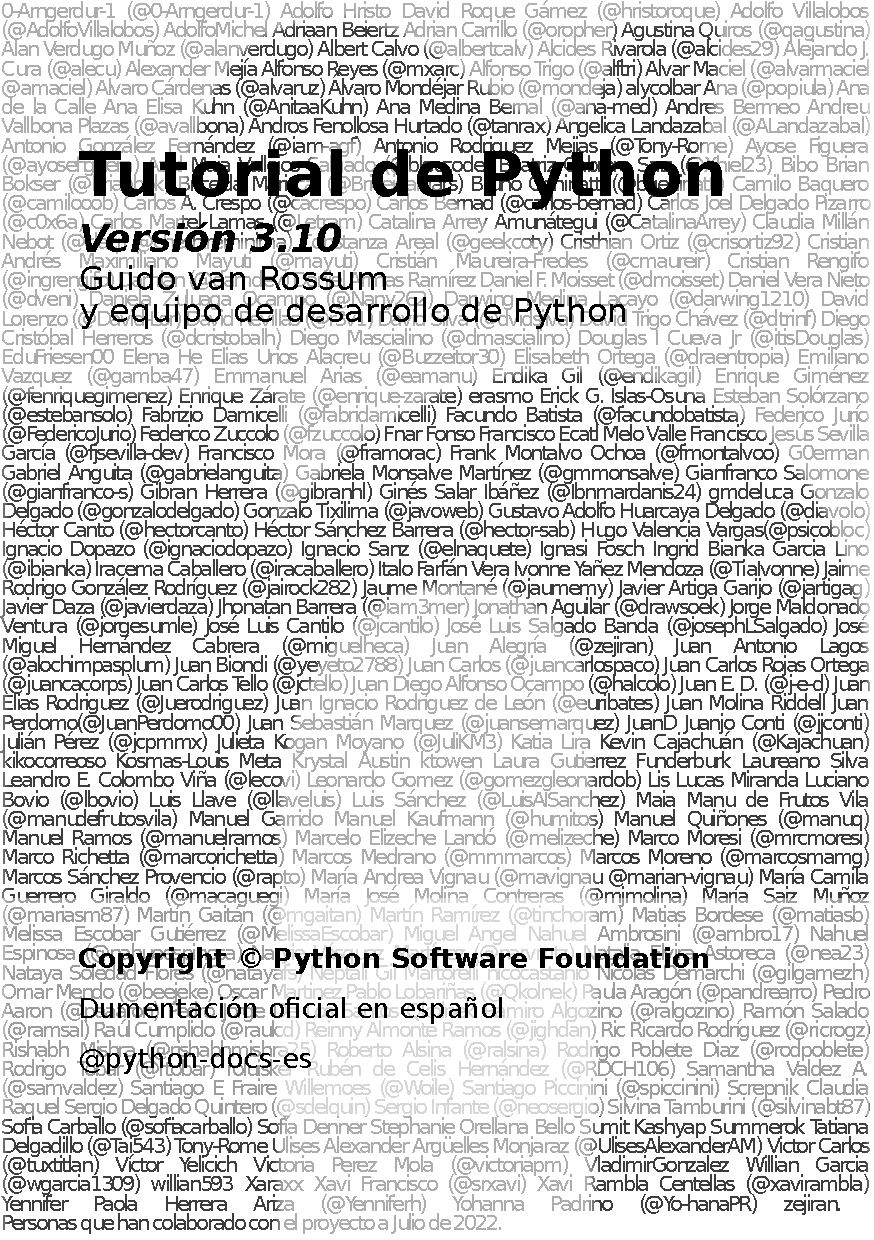
\includepdf[pages=-]{portada/cover-logo.pdf}
\pagestyle{plain}
\sphinxtableofcontents
\pagestyle{normal}
\phantomsection\label{\detokenize{tutorial/index::doc}}


\sphinxAtStartPar
Python es un lenguaje de programación potente y fácil de aprender. Tiene estructuras de datos de alto nivel eficientes y un simple pero efectivo sistema de programación orientado a objetos. La elegante sintaxis de Python y su tipado dinámico, junto a su naturaleza interpretada lo convierten en un lenguaje ideal para scripting y desarrollo rápido de aplicaciones en muchas áreas, para la mayoría de plataformas.

\sphinxAtStartPar
El intérprete de Python y la extensa librería estándar se encuentran disponibles libremente en código fuente y de forma binaria para la mayoría de las plataformas desde la Web de Python, \sphinxurl{https://www.python.org/}, y se pueden distribuir libremente. El mismo sitio también contiene distribuciones y referencias a muchos módulos libres de Python de terceros, programas, herramientas y documentación adicional.

\sphinxAtStartPar
El intérprete de Python es fácilmente extensible con funciones y tipos de datos implementados en C o C++ (u otros lenguajes que permitan ser llamados desde C). Python también es apropiado como un lenguaje para extender aplicaciones modificables.

\sphinxAtStartPar
Este tutorial introduce al lector informalmente a los conceptos básicos y las funcionalidades del lenguaje de programación Python y a su sistema. Ayuda tener un interprete de Python accesible para una experiencia práctica, todos los ejemplos son auto\sphinxhyphen{}contenidos, permitiendo utilizar el tutorial sin conexión.

\sphinxAtStartPar
No busca ser exhaustivo ni cubrir cada una de las características del lenguaje, ni siquiera las más utilizadas. En vez de eso, pretende introducir muchas de las funcionalidades más notables y brindar una idea clara acerca del estilo y el tipo de lenguaje que es Python. 

\sphinxAtStartPar
Después de leer este material podrás leer y escribir módulos y programas en Python. ¡Estarás listo para aprender más acerca de las diversas bibliotecas y módulos!


\chapter{Abriendo el apetito}
\label{\detokenize{tutorial/appetite:whetting-your-appetite}}\label{\detokenize{tutorial/appetite:tut-intro}}\label{\detokenize{tutorial/appetite::doc}}
\sphinxAtStartPar
Si trabajas mucho con ordenadores, en algún momento encontrarás que hay alguna tarea que quieres automatizar. Por ejemplo, quizás quieres buscar y remplazar un texto en muchos ficheros o renombrar y reordenar un montón de imágenes de forma complicada. Quizás lo que quieres es escribir una pequeña base de datos personalizada, una interfaz gráfica o un juego simple.

\sphinxAtStartPar
Si eres un desarrollador profesional, quizás quieres trabajar con varias librerías de C/C++/Java pero encuentras el ciclo de escribir/compilar/probar/recompilar bastante lento. Quizás estás escribiendo una serie de pruebas para éstas librerías y te parece tedioso escribir el código de pruebas. O quizás has escrito un programa que puede utilizar un lenguaje como extensión y no quieres diseñar e implementar un lenguaje entero para tu aplicación.

\sphinxAtStartPar
Python es justo el lenguaje para ti.

\sphinxAtStartPar
Puede escribir un script de shell de Unix o archivos por lotes de Windows para algunas de estas tareas, pero los scripts de shell son mejores para mover archivos y cambiar datos de texto, no son adecuados para juegos o aplicaciones GUI. Podría escribir un programa C / C ++ / Java, pero puede llevar mucho tiempo de desarrollo obtener incluso un programa de primer borrador. Python es más fácil de usar, está disponible en los sistemas operativos Windows, macOS y Unix, y lo ayudará a hacer el trabajo más rápidamente.

\sphinxAtStartPar
Python es fácil de utilizar siendo un lenguaje de programación real ofreciendo mucha más estructura y soporte para programas grandes que la que ofrecen shell scripts o ficheros batch. Por otro lado, Python también ofrece mayor comprobación de errores que C y siendo un \sphinxstyleemphasis{lenguaje de muy alto nivel} tiene tipos de datos de alto nivel incorporados como listas flexibles y diccionarios. Debido a sus tipos de datos más generales, Python es aplicable a más dominios que Awk o Perl, aunque hay muchas cosas que son tan sencillas en Python como en esos lenguajes.

\sphinxAtStartPar
Python te permite dividir tu programa en módulos que pueden reutilizarse en otros programas de Python. Tiene una gran colección de módulos estándar que puedes utilizar como la base de tus programas o como ejemplos para empezar a aprender Python. Algunos de estos módulos proporcionan cosas como entrada/salida de ficheros, llamadas a sistema, sockets e incluso interfaces a herramientas de interfaz gráfica como Tk.

\sphinxAtStartPar
Python es un lenguaje interpretado, lo cual puede ahorrarte mucho tiempo durante el desarrollo ya que no es necesario compilar ni enlazar. El intérprete puede usarse interactivamente, lo que facilita experimentar con características del lenguaje, escribir programas desechables o probar funciones cuando se hace desarrollo de programas de abajo hacia arriba. Es también una calculadora de escritorio práctica.

\sphinxAtStartPar
Python permite escribir programas compactos y legibles. Los programas en Python son típicamente más cortos que sus programas equivalentes en C, C++ o Java por varios motivos:
\begin{itemize}
\item {} 
\sphinxAtStartPar
los tipos de datos de alto nivel permiten expresar operaciones complejas en una sola instrucción;

\item {} 
\sphinxAtStartPar
la agrupación de instrucciones se hace mediante indentación en vez de llaves de apertura y cierre;

\item {} 
\sphinxAtStartPar
no es necesario declarar variables ni argumentos.

\end{itemize}

\sphinxAtStartPar
Python es \sphinxstyleemphasis{extensible}: si ya sabes programar en C es fácil añadir nuevas funciones o módulos al intérprete, ya sea para realizar operaciones críticas a velocidad máxima, o para enlazar programas de Python con bibliotecas que tal vez sólo estén disponibles de forma binaria (por ejemplo bibliotecas gráficas específicas de un fabricante). Una vez estés realmente entusiasmado, puedes enlazar el intérprete Python en una aplicación hecha en C y usarlo como lenguaje de extensión o de comando para esa aplicación.

\sphinxAtStartPar
Por cierto, el lenguaje recibe su nombre del programa de televisión de la BBC «Monty Python’s Flying Circus» y no tiene nada que ver con reptiles. Hacer referencias sobre Monty Python en la documentación no sólo esta permitido, ¡sino que también está bien visto!

\sphinxAtStartPar
Ahora que estás emocionado con Python, querrás verlo en más detalle. Como la mejor forma de aprender un lenguaje es usarlo, el tutorial te invita a que juegues con el intérprete de Python a medida que vas leyendo.

\sphinxAtStartPar
En el próximo capítulo se explicará la mecánica de uso del intérprete. Esta es información bastante mundana, pero es esencial para poder probar los ejemplos que aparecerán más adelante.

\sphinxAtStartPar
El resto del tutorial introduce varias características del lenguaje y el sistema Python a través de ejemplos, empezando con expresiones, instrucciones y tipos de datos simples, pasando por funciones y módulos, y finalmente tocando conceptos avanzados como excepciones y clases definidas por el usuario.


\chapter{Usando el intérprete de Python}
\label{\detokenize{tutorial/interpreter:using-the-python-interpreter}}\label{\detokenize{tutorial/interpreter:tut-using}}\label{\detokenize{tutorial/interpreter::doc}}

\section{Invocando al intérprete}
\label{\detokenize{tutorial/interpreter:invoking-the-interpreter}}\label{\detokenize{tutorial/interpreter:tut-invoking}}
\sphinxAtStartPar
El intérprete de Python generalmente se instala como \sphinxcode{\sphinxupquote{/usr/local/bin/python3.10}} en aquellas máquinas donde está disponible; poner \sphinxcode{\sphinxupquote{/usr/local/bin}} en la ruta de búsqueda de su shell de Unix hace posible iniciarlo escribiendo el comando:

\begin{sphinxVerbatim}[commandchars=\\\{\}]
python3.10
\end{sphinxVerbatim}

\sphinxAtStartPar
en el terminal %
\begin{footnote}[1]\sphinxAtStartFootnote
En Unix, el intérprete de Python 3.x no está instalado por defecto con el ejecutable llamado \sphinxcode{\sphinxupquote{python}}, por lo que no entra en conflicto con un ejecutable de Python 2.x instalado simultáneamente.
%
\end{footnote}. Ya que la elección del directorio dónde vivirá el intérprete es una opción del proceso de instalación, puede estar en otros lugares; consulta a tu experto Python local o administrador de sistemas. (Por ejemplo, \sphinxcode{\sphinxupquote{/usr/local/python}} es una alternativa popular).

\sphinxAtStartPar
En máquinas con Windows en las que haya instalado Python desde \DUrole{xref,std,std-ref}{Microsoft Store}, el comando \sphinxcode{\sphinxupquote{python3.10}} estará disponible. Si tiene el \DUrole{xref,std,std-ref}{lanzador py.exe} instalado, puede usar el comando \sphinxcode{\sphinxupquote{py}}. Consulte \DUrole{xref,std,std-ref}{setting\sphinxhyphen{}envvars} para conocer otras formas de iniciar Python.

\sphinxAtStartPar
Se puede salir del intérprete con estado de salida cero ingresando el carácter de fin de archivo (\sphinxkeyboard{\sphinxupquote{Control\sphinxhyphen{}D}} en Unix, \sphinxkeyboard{\sphinxupquote{Control\sphinxhyphen{}Z}} en Windows). Si eso no funciona, puedes salir del intérprete escribiendo el comando: \sphinxcode{\sphinxupquote{quit()}}.

\sphinxAtStartPar
Las características para edición de líneas del intérprete incluyen edición interactiva, sustitución de historial y completado de código en sistemas que soportan \sphinxhref{https://tiswww.case.edu/php/chet/readline/rltop.html}{GNU Readline} librería. Quizás la forma más rápida para comprobar si las características de edición se encuentran disponibles es escribir \sphinxkeyboard{\sphinxupquote{Control\sphinxhyphen{}P}} en el primer prompt de Python que aparezca. Si se escucha un sonido, tienes edición de línea de comandos; ver Apéndice {\hyperref[\detokenize{tutorial/interactive:tut-interacting}]{\sphinxcrossref{\DUrole{std,std-ref}{Edición de entrada interactiva y sustitución de historial}}}} para una introducción a las teclas. Si no parece que ocurra nada, o si se muestra \sphinxcode{\sphinxupquote{\textasciicircum{}P}}, estas características no están disponibles; solo vas a poder usar la tecla de retroceso (\sphinxstyleemphasis{backspace}) para borrar los caracteres de la línea actual.

\sphinxAtStartPar
El intérprete funciona de manera similar al shell de Unix: cuando se le llama con una entrada estándar conectada a un terminal, lee y ejecuta comandos de manera interactiva; cuando se le llama con un argumento de nombre de archivo o con un archivo como entrada estándar, lee y ejecuta un \sphinxstyleemphasis{script} desde ese archivo.

\sphinxAtStartPar
Una segunda forma de iniciar el intérprete es \sphinxcode{\sphinxupquote{python \sphinxhyphen{}c comando {[}arg{]} ...}}, que ejecuta las sentencias en \sphinxstyleemphasis{comando}, similar a la opción de shell \sphinxcode{\sphinxupquote{\sphinxhyphen{}c}} . Como las sentencias de Python a menudo contienen espacios u otros caracteres que son especiales para el shell, generalmente se recomienda citar \sphinxstyleemphasis{comando} con comillas simples.

\sphinxAtStartPar
Algunos módulos de Python también son útiles como scripts. Estos pueden invocarse utilizando \sphinxcode{\sphinxupquote{python \sphinxhyphen{}m module {[}arg{]} ...}}, que ejecuta el archivo fuente para \sphinxstyleemphasis{module} como si se hubiera escrito el nombre completo en la línea de comandos.

\sphinxAtStartPar
Cuando se usa un script, a veces es útil poder ejecutar el script y luego ingresar al modo interactivo. Esto se puede hacer pasando la \sphinxcode{\sphinxupquote{\sphinxhyphen{}i}} antes del nombre del script.

\sphinxAtStartPar
Todas las opciones de la línea de comandos se describen en \DUrole{xref,std,std-ref}{using\sphinxhyphen{}on\sphinxhyphen{}general}.


\subsection{Paso de argumentos}
\label{\detokenize{tutorial/interpreter:argument-passing}}\label{\detokenize{tutorial/interpreter:tut-argpassing}}
\sphinxAtStartPar
Cuando son conocidos por el intérprete, el nombre del script y los argumentos adicionales se convierten a una lista de cadenas de texto asignada a la variable \sphinxcode{\sphinxupquote{argv}} del módulo \sphinxcode{\sphinxupquote{sys}}. Puedes acceder a esta lista haciendo \sphinxcode{\sphinxupquote{import sys}}. La longitud de la lista es al menos uno; cuando no se utiliza ningún script o argumento, \sphinxcode{\sphinxupquote{sys.argv{[}0{]}}} es una cadena vacía. Cuando se pasa el nombre del script con \sphinxcode{\sphinxupquote{'\sphinxhyphen{}'}} (lo que significa la entrada estándar), \sphinxcode{\sphinxupquote{sys.argv{[}0{]}}} vale \sphinxcode{\sphinxupquote{'\sphinxhyphen{}'}}. Cuando se usa \sphinxcode{\sphinxupquote{\sphinxhyphen{}c}} \sphinxstyleemphasis{comando}, \sphinxcode{\sphinxupquote{sys.argv{[}0{]}}} vale \sphinxcode{\sphinxupquote{'\sphinxhyphen{}c'}}. Cuando se usa \sphinxcode{\sphinxupquote{\sphinxhyphen{}m}} \sphinxstyleemphasis{módulo}, \sphinxcode{\sphinxupquote{sys.argv{[}0{]}}} contiene el valor del nombre completo del módulo. Las opciones encontradas después de \sphinxcode{\sphinxupquote{\sphinxhyphen{}c}} \sphinxstyleemphasis{comand} o \sphinxcode{\sphinxupquote{\sphinxhyphen{}m}} \sphinxstyleemphasis{módulo} no son consumidas por el procesador de opciones de Python pero de todas formas se almacenan en \sphinxcode{\sphinxupquote{sys.argv}} para ser manejadas por el comando o módulo.


\subsection{Modo interactivo}
\label{\detokenize{tutorial/interpreter:interactive-mode}}\label{\detokenize{tutorial/interpreter:tut-interactive}}
\sphinxAtStartPar
Cuando se leen los comandos desde un terminal, se dice que el intérprete está en \sphinxstyleemphasis{modo interactivo}. En este modo, espera el siguiente comando con el \sphinxstyleemphasis{prompt primario}, generalmente tres signos de mayor que (\sphinxcode{\sphinxupquote{>>>}}); para las líneas de continuación, aparece el \sphinxstyleemphasis{prompt secundario}, por defecto tres puntos (\sphinxcode{\sphinxupquote{...}}). El intérprete imprime un mensaje de bienvenida que indica su número de versión y un aviso de copyright antes de imprimir el primer \sphinxstyleemphasis{prompt primario}:

\begin{sphinxVerbatim}[commandchars=\\\{\}]
\PYG{g+gp}{\PYGZdl{}} python3.10
\PYG{g+go}{Python 3.10 (default, June 4 2019, 09:25:04)}
\PYG{g+go}{[GCC 4.8.2] on linux}
\PYG{g+go}{Type \PYGZdq{}help\PYGZdq{}, \PYGZdq{}copyright\PYGZdq{}, \PYGZdq{}credits\PYGZdq{} or \PYGZdq{}license\PYGZdq{} for more information.}
\PYG{g+gp}{\PYGZgt{}}\PYGZgt{}\PYGZgt{}
\end{sphinxVerbatim}

\sphinxAtStartPar
Las líneas de continuación son necesarias cuando se ingresa una construcción multilínea. Como ejemplo, echa un vistazo a la sentencia \sphinxcode{\sphinxupquote{if}}:

\begin{sphinxVerbatim}[commandchars=\\\{\}]
\PYG{g+gp}{\PYGZgt{}\PYGZgt{}\PYGZgt{} }\PYG{n}{the\PYGZus{}world\PYGZus{}is\PYGZus{}flat} \PYG{o}{=} \PYG{k+kc}{True}
\PYG{g+gp}{\PYGZgt{}\PYGZgt{}\PYGZgt{} }\PYG{k}{if} \PYG{n}{the\PYGZus{}world\PYGZus{}is\PYGZus{}flat}\PYG{p}{:}
\PYG{g+gp}{... }    \PYG{n+nb}{print}\PYG{p}{(}\PYG{l+s+s2}{\PYGZdq{}}\PYG{l+s+s2}{Be careful not to fall off!}\PYG{l+s+s2}{\PYGZdq{}}\PYG{p}{)}
\PYG{g+gp}{...}
\PYG{g+go}{Be careful not to fall off!}
\end{sphinxVerbatim}

\sphinxAtStartPar
Para más información sobre el modo interactivo, ver {\hyperref[\detokenize{tutorial/appendix:tut-interac}]{\sphinxcrossref{\DUrole{std,std-ref}{Modo interactivo}}}}.


\section{El intérprete y su entorno}
\label{\detokenize{tutorial/interpreter:the-interpreter-and-its-environment}}\label{\detokenize{tutorial/interpreter:tut-interp}}

\subsection{Codificación del código fuente}
\label{\detokenize{tutorial/interpreter:source-code-encoding}}\label{\detokenize{tutorial/interpreter:tut-source-encoding}}
\sphinxAtStartPar
De forma predeterminada, los archivos fuente de Python se tratan como codificados en UTF\sphinxhyphen{}8. En esa codificación, los caracteres de la mayoría de los idiomas del mundo se pueden usar simultáneamente en literales, identificadores y comentarios, aunque la biblioteca estándar solo usa caracteres ASCII para los identificadores, una convención que debería seguir cualquier código que sea portable.Para mostrar todos estos caracteres correctamente, tu editor debe reconocer que el archivo es UTF\sphinxhyphen{}8, y debe usar una fuente que admita todos los caracteres del archivo.

\sphinxAtStartPar
Para declarar una codificación que no sea la predeterminada, se debe agregar una línea de comentario especial como la \sphinxstyleemphasis{primera} línea del archivo. La sintaxis es la siguiente:

\begin{sphinxVerbatim}[commandchars=\\\{\}]
\PYG{c+c1}{\PYGZsh{} \PYGZhy{}*\PYGZhy{} coding: encoding \PYGZhy{}*\PYGZhy{}}
\end{sphinxVerbatim}

\sphinxAtStartPar
donde \sphinxstyleemphasis{codificación} es uno de los \sphinxcode{\sphinxupquote{codecs}} soportados por Python.

\sphinxAtStartPar
Por ejemplo, para declarar que se utilizará la codificación de Windows\sphinxhyphen{}1252, la primera línea del archivo de código fuente debe ser:

\begin{sphinxVerbatim}[commandchars=\\\{\}]
\PYG{c+c1}{\PYGZsh{} \PYGZhy{}*\PYGZhy{} coding: cp1252 \PYGZhy{}*\PYGZhy{}}
\end{sphinxVerbatim}

\sphinxAtStartPar
Una excepción a la regla de \sphinxstyleemphasis{primera línea} es cuando el código fuente comienza con una línea {\hyperref[\detokenize{tutorial/appendix:tut-scripts}]{\sphinxcrossref{\DUrole{std,std-ref}{UNIX «shebang» line}}}}. En ese caso, la declaración de codificación debe agregarse como la segunda línea del archivo. Por ejemplo:

\begin{sphinxVerbatim}[commandchars=\\\{\}]
\PYG{c+ch}{\PYGZsh{}!/usr/bin/env python3}
\PYG{c+c1}{\PYGZsh{} \PYGZhy{}*\PYGZhy{} coding: cp1252 \PYGZhy{}*\PYGZhy{}}
\end{sphinxVerbatim}


\chapter{Una introducción informal a Python}
\label{\detokenize{tutorial/introduction:an-informal-introduction-to-python}}\label{\detokenize{tutorial/introduction:tut-informal}}\label{\detokenize{tutorial/introduction::doc}}
\sphinxAtStartPar
En los siguientes ejemplos, la entrada y la salida se distinguen por la presencia o ausencia de prompts ({\hyperref[\detokenize{glossary:term-0}]{\sphinxtermref{\DUrole{xref,std,std-term}{>>>}}}} y {\hyperref[\detokenize{glossary:term-...}]{\sphinxtermref{\DUrole{xref,std,std-term}{…}}}}): para repetir el ejemplo, escribe todo después del prompt, cuando aparece; las líneas que no comienzan con un prompt son emitidas desde el intérprete. Ten en cuenta que un prompt secundario solo en una linea de ejemplo significa que debes escribir una línea en blanco. Esto se utiliza para finalizar un comando multilínea.

\index{\# (hash)@\spxentry{\#}\spxextra{hash}!comment@\spxentry{comment}}\ignorespaces 
\sphinxAtStartPar
Muchos de los ejemplos de este manual, incluso aquellos ingresados en el prompt interactivo, incluyen comentarios. Los comentarios en Python comienzan con el carácter numeral, \sphinxcode{\sphinxupquote{\#}}, y se extienden hasta el final visible de la línea. Un comentario quizás aparezca al comienzo de la línea o seguido de espacios en blanco o código, pero no dentro de una cadena de caracteres. Un carácter numeral dentro de una cadena de caracteres es sólo un carácter numeral. Ya que los comentarios son para aclarar código y no son interpretados por Python, pueden omitirse cuando se escriben los ejemplos.

\sphinxAtStartPar
Algunos ejemplos:

\begin{sphinxVerbatim}[commandchars=\\\{\}]
\PYG{c+c1}{\PYGZsh{} this is the first comment}
\PYG{n}{spam} \PYG{o}{=} \PYG{l+m+mi}{1}  \PYG{c+c1}{\PYGZsh{} and this is the second comment}
          \PYG{c+c1}{\PYGZsh{} ... and now a third!}
\PYG{n}{text} \PYG{o}{=} \PYG{l+s+s2}{\PYGZdq{}}\PYG{l+s+s2}{\PYGZsh{} This is not a comment because it}\PYG{l+s+s2}{\PYGZsq{}}\PYG{l+s+s2}{s inside quotes.}\PYG{l+s+s2}{\PYGZdq{}}
\end{sphinxVerbatim}


\section{Usando Python como una calculadora}
\label{\detokenize{tutorial/introduction:using-python-as-a-calculator}}\label{\detokenize{tutorial/introduction:tut-calculator}}
\sphinxAtStartPar
Probemos algunos comandos simples de Python. Inicia el intérprete y espere el prompt primario, \sphinxcode{\sphinxupquote{>>>}}. (No debería tardar mucho.)


\subsection{Números}
\label{\detokenize{tutorial/introduction:numbers}}\label{\detokenize{tutorial/introduction:tut-numbers}}
\sphinxAtStartPar
El intérprete puede utilizarse como una simple calculadora; puedes introducir una expresión y este escribirá los valores. La sintaxis es sencilla: los operadores \sphinxcode{\sphinxupquote{+}}, \sphinxcode{\sphinxupquote{\sphinxhyphen{}}}, \sphinxcode{\sphinxupquote{*}} y \sphinxcode{\sphinxupquote{/``funcionan como en la mayoría de los lenguajes (por ejemplo, Pascal o C); los paréntesis (``()}}) pueden ser usados para agrupar. Por ejemplo:

\begin{sphinxVerbatim}[commandchars=\\\{\}]
\PYG{g+gp}{\PYGZgt{}\PYGZgt{}\PYGZgt{} }\PYG{l+m+mi}{2} \PYG{o}{+} \PYG{l+m+mi}{2}
\PYG{g+go}{4}
\PYG{g+gp}{\PYGZgt{}\PYGZgt{}\PYGZgt{} }\PYG{l+m+mi}{50} \PYG{o}{\PYGZhy{}} \PYG{l+m+mi}{5}\PYG{o}{*}\PYG{l+m+mi}{6}
\PYG{g+go}{20}
\PYG{g+gp}{\PYGZgt{}\PYGZgt{}\PYGZgt{} }\PYG{p}{(}\PYG{l+m+mi}{50} \PYG{o}{\PYGZhy{}} \PYG{l+m+mi}{5}\PYG{o}{*}\PYG{l+m+mi}{6}\PYG{p}{)} \PYG{o}{/} \PYG{l+m+mi}{4}
\PYG{g+go}{5.0}
\PYG{g+gp}{\PYGZgt{}\PYGZgt{}\PYGZgt{} }\PYG{l+m+mi}{8} \PYG{o}{/} \PYG{l+m+mi}{5}  \PYG{c+c1}{\PYGZsh{} division always returns a floating point number}
\PYG{g+go}{1.6}
\end{sphinxVerbatim}

\sphinxAtStartPar
Los números enteros (ej. \sphinxcode{\sphinxupquote{2}}, \sphinxcode{\sphinxupquote{4}}, \sphinxcode{\sphinxupquote{20}}) tienen tipo \sphinxcode{\sphinxupquote{int}}, los que tienen una parte fraccionaria (por ejemplo \sphinxcode{\sphinxupquote{5.0}}, \sphinxcode{\sphinxupquote{1.6}}) tiene el tipo \sphinxcode{\sphinxupquote{float}}. Vamos a ver más acerca de los tipos numéricos más adelante en el tutorial.

\sphinxAtStartPar
La división (\sphinxcode{\sphinxupquote{/}}) siempre retorna un punto flotante. Para hacer {\hyperref[\detokenize{glossary:term-floor-division}]{\sphinxtermref{\DUrole{xref,std,std-term}{floor division}}}} y obtener un resultado entero (descartando cualquier resultado fraccionario) puede usarse el operador \sphinxcode{\sphinxupquote{//}}; para calcular el resto puedes usar \sphinxcode{\sphinxupquote{\%}}:

\begin{sphinxVerbatim}[commandchars=\\\{\}]
\PYG{g+gp}{\PYGZgt{}\PYGZgt{}\PYGZgt{} }\PYG{l+m+mi}{17} \PYG{o}{/} \PYG{l+m+mi}{3}  \PYG{c+c1}{\PYGZsh{} classic division returns a float}
\PYG{g+go}{5.666666666666667}
\PYG{g+go}{\PYGZgt{}\PYGZgt{}\PYGZgt{}}
\PYG{g+gp}{\PYGZgt{}\PYGZgt{}\PYGZgt{} }\PYG{l+m+mi}{17} \PYG{o}{/}\PYG{o}{/} \PYG{l+m+mi}{3}  \PYG{c+c1}{\PYGZsh{} floor division discards the fractional part}
\PYG{g+go}{5}
\PYG{g+gp}{\PYGZgt{}\PYGZgt{}\PYGZgt{} }\PYG{l+m+mi}{17} \PYG{o}{\PYGZpc{}} \PYG{l+m+mi}{3}  \PYG{c+c1}{\PYGZsh{} the \PYGZpc{} operator returns the remainder of the division}
\PYG{g+go}{2}
\PYG{g+gp}{\PYGZgt{}\PYGZgt{}\PYGZgt{} }\PYG{l+m+mi}{5} \PYG{o}{*} \PYG{l+m+mi}{3} \PYG{o}{+} \PYG{l+m+mi}{2}  \PYG{c+c1}{\PYGZsh{} floored quotient * divisor + remainder}
\PYG{g+go}{17}
\end{sphinxVerbatim}

\sphinxAtStartPar
Con Python, es posible usar el operador \sphinxcode{\sphinxupquote{**}} para calcular potencias %
\begin{footnote}[1]\sphinxAtStartFootnote
Debido a que \sphinxcode{\sphinxupquote{**}} tiene una prioridad mayor que \sphinxcode{\sphinxupquote{`\sphinxhyphen{}}}, \sphinxcode{\sphinxupquote{\sphinxhyphen{}3**2}} se interpretará como \sphinxcode{\sphinxupquote{\sphinxhyphen{}(3**2)}}, por lo tanto dará como resultado \sphinxcode{\sphinxupquote{\sphinxhyphen{}9}}. Para evitar esto y obtener \sphinxcode{\sphinxupquote{9}}, puedes usar \sphinxcode{\sphinxupquote{(\sphinxhyphen{}3)**2}}.
%
\end{footnote}:

\begin{sphinxVerbatim}[commandchars=\\\{\}]
\PYG{g+gp}{\PYGZgt{}\PYGZgt{}\PYGZgt{} }\PYG{l+m+mi}{5} \PYG{o}{*}\PYG{o}{*} \PYG{l+m+mi}{2}  \PYG{c+c1}{\PYGZsh{} 5 squared}
\PYG{g+go}{25}
\PYG{g+gp}{\PYGZgt{}\PYGZgt{}\PYGZgt{} }\PYG{l+m+mi}{2} \PYG{o}{*}\PYG{o}{*} \PYG{l+m+mi}{7}  \PYG{c+c1}{\PYGZsh{} 2 to the power of 7}
\PYG{g+go}{128}
\end{sphinxVerbatim}

\sphinxAtStartPar
El signo igual (\sphinxcode{\sphinxupquote{=}}) se usa para asignar un valor a una variable. Ningún resultado se mostrará antes del siguiente prompt interactivo:

\begin{sphinxVerbatim}[commandchars=\\\{\}]
\PYG{g+gp}{\PYGZgt{}\PYGZgt{}\PYGZgt{} }\PYG{n}{width} \PYG{o}{=} \PYG{l+m+mi}{20}
\PYG{g+gp}{\PYGZgt{}\PYGZgt{}\PYGZgt{} }\PYG{n}{height} \PYG{o}{=} \PYG{l+m+mi}{5} \PYG{o}{*} \PYG{l+m+mi}{9}
\PYG{g+gp}{\PYGZgt{}\PYGZgt{}\PYGZgt{} }\PYG{n}{width} \PYG{o}{*} \PYG{n}{height}
\PYG{g+go}{900}
\end{sphinxVerbatim}

\sphinxAtStartPar
Si una variable no está «definida» (no se le ha asignado un valor), al intentar usarla dará un error:

\begin{sphinxVerbatim}[commandchars=\\\{\}]
\PYG{g+gp}{\PYGZgt{}\PYGZgt{}\PYGZgt{} }\PYG{n}{n}  \PYG{c+c1}{\PYGZsh{} try to access an undefined variable}
\PYG{g+gt}{Traceback (most recent call last):}
  File \PYG{n+nb}{\PYGZdq{}\PYGZlt{}stdin\PYGZgt{}\PYGZdq{}}, line \PYG{l+m}{1}, in \PYG{n}{\PYGZlt{}module\PYGZgt{}}
\PYG{g+gr}{NameError}: \PYG{n}{name \PYGZsq{}n\PYGZsq{} is not defined}
\end{sphinxVerbatim}

\sphinxAtStartPar
Hay soporte completo de punto flotante; operadores con operando mezclados convertirán los enteros a punto flotante:

\begin{sphinxVerbatim}[commandchars=\\\{\}]
\PYG{g+gp}{\PYGZgt{}\PYGZgt{}\PYGZgt{} }\PYG{l+m+mi}{4} \PYG{o}{*} \PYG{l+m+mf}{3.75} \PYG{o}{\PYGZhy{}} \PYG{l+m+mi}{1}
\PYG{g+go}{14.0}
\end{sphinxVerbatim}

\sphinxAtStartPar
En el modo interactivo, la última expresión impresa se asigna a la variable \sphinxcode{\sphinxupquote{\_}}.  Esto significa que cuando se está utilizando Python como calculadora, es más fácil seguir calculando, por ejemplo:

\begin{sphinxVerbatim}[commandchars=\\\{\}]
\PYG{g+gp}{\PYGZgt{}\PYGZgt{}\PYGZgt{} }\PYG{n}{tax} \PYG{o}{=} \PYG{l+m+mf}{12.5} \PYG{o}{/} \PYG{l+m+mi}{100}
\PYG{g+gp}{\PYGZgt{}\PYGZgt{}\PYGZgt{} }\PYG{n}{price} \PYG{o}{=} \PYG{l+m+mf}{100.50}
\PYG{g+gp}{\PYGZgt{}\PYGZgt{}\PYGZgt{} }\PYG{n}{price} \PYG{o}{*} \PYG{n}{tax}
\PYG{g+go}{12.5625}
\PYG{g+gp}{\PYGZgt{}\PYGZgt{}\PYGZgt{} }\PYG{n}{price} \PYG{o}{+} \PYG{n}{\PYGZus{}}
\PYG{g+go}{113.0625}
\PYG{g+gp}{\PYGZgt{}\PYGZgt{}\PYGZgt{} }\PYG{n+nb}{round}\PYG{p}{(}\PYG{n}{\PYGZus{}}\PYG{p}{,} \PYG{l+m+mi}{2}\PYG{p}{)}
\PYG{g+go}{113.06}
\end{sphinxVerbatim}

\sphinxAtStartPar
Esta variable debe ser tratada como de sólo lectura por el usuario. No le asignes explícitamente un valor; crearás una variable local independiente con el mismo nombre enmascarando la variable con el comportamiento mágico.

\sphinxAtStartPar
Además de \sphinxcode{\sphinxupquote{int}} y \sphinxcode{\sphinxupquote{float}}, Python admite otros tipos de números, como \sphinxcode{\sphinxupquote{Decimal}} y \sphinxcode{\sphinxupquote{Fraction}}. Python también tiene soporte incorporado para \DUrole{xref,std,std-ref}{complex numbers}, y usa el sufijo \sphinxcode{\sphinxupquote{j}} o \sphinxcode{\sphinxupquote{J}} para indicar la parte imaginaria (por ejemplo, \sphinxcode{\sphinxupquote{3+5j}}).


\subsection{Cadenas de caracteres}
\label{\detokenize{tutorial/introduction:strings}}\label{\detokenize{tutorial/introduction:tut-strings}}
\sphinxAtStartPar
Además de números, Python puede manipular cadenas de texto, las cuales pueden ser expresadas de distintas formas. Pueden estar encerradas en comillas simples (\sphinxcode{\sphinxupquote{'...'}}) o dobles (\sphinxcode{\sphinxupquote{"..."}})  con el mismo resultado %
\begin{footnote}[2]\sphinxAtStartFootnote
A diferencia de otros lenguajes, caracteres especiales como \sphinxcode{\sphinxupquote{\textbackslash{}n}} tienen el mismo significado con simple(\sphinxcode{\sphinxupquote{'...'}}) y dobles (\sphinxcode{\sphinxupquote{"..."}}) comillas. La única diferencia entre las dos es que dentro de las comillas simples no existe la necesidad de escapar \sphinxcode{\sphinxupquote{"}} (pero tienes que escapar \sphinxcode{\sphinxupquote{\textbackslash{}'}}) y viceversa.
%
\end{footnote}.  \sphinxcode{\sphinxupquote{\textbackslash{}}} puede ser usado para escapar comillas:

\begin{sphinxVerbatim}[commandchars=\\\{\}]
\PYG{g+gp}{\PYGZgt{}\PYGZgt{}\PYGZgt{} }\PYG{l+s+s1}{\PYGZsq{}}\PYG{l+s+s1}{spam eggs}\PYG{l+s+s1}{\PYGZsq{}}  \PYG{c+c1}{\PYGZsh{} single quotes}
\PYG{g+go}{\PYGZsq{}spam eggs\PYGZsq{}}
\PYG{g+gp}{\PYGZgt{}\PYGZgt{}\PYGZgt{} }\PYG{l+s+s1}{\PYGZsq{}}\PYG{l+s+s1}{doesn}\PYG{l+s+se}{\PYGZbs{}\PYGZsq{}}\PYG{l+s+s1}{t}\PYG{l+s+s1}{\PYGZsq{}}  \PYG{c+c1}{\PYGZsh{} use \PYGZbs{}\PYGZsq{} to escape the single quote...}
\PYG{g+go}{\PYGZdq{}doesn\PYGZsq{}t\PYGZdq{}}
\PYG{g+gp}{\PYGZgt{}\PYGZgt{}\PYGZgt{} }\PYG{l+s+s2}{\PYGZdq{}}\PYG{l+s+s2}{doesn}\PYG{l+s+s2}{\PYGZsq{}}\PYG{l+s+s2}{t}\PYG{l+s+s2}{\PYGZdq{}}  \PYG{c+c1}{\PYGZsh{} ...or use double quotes instead}
\PYG{g+go}{\PYGZdq{}doesn\PYGZsq{}t\PYGZdq{}}
\PYG{g+gp}{\PYGZgt{}\PYGZgt{}\PYGZgt{} }\PYG{l+s+s1}{\PYGZsq{}}\PYG{l+s+s1}{\PYGZdq{}}\PYG{l+s+s1}{Yes,}\PYG{l+s+s1}{\PYGZdq{}}\PYG{l+s+s1}{ they said.}\PYG{l+s+s1}{\PYGZsq{}}
\PYG{g+go}{\PYGZsq{}\PYGZdq{}Yes,\PYGZdq{} they said.\PYGZsq{}}
\PYG{g+gp}{\PYGZgt{}\PYGZgt{}\PYGZgt{} }\PYG{l+s+s2}{\PYGZdq{}}\PYG{l+s+se}{\PYGZbs{}\PYGZdq{}}\PYG{l+s+s2}{Yes,}\PYG{l+s+se}{\PYGZbs{}\PYGZdq{}}\PYG{l+s+s2}{ they said.}\PYG{l+s+s2}{\PYGZdq{}}
\PYG{g+go}{\PYGZsq{}\PYGZdq{}Yes,\PYGZdq{} they said.\PYGZsq{}}
\PYG{g+gp}{\PYGZgt{}\PYGZgt{}\PYGZgt{} }\PYG{l+s+s1}{\PYGZsq{}}\PYG{l+s+s1}{\PYGZdq{}}\PYG{l+s+s1}{Isn}\PYG{l+s+se}{\PYGZbs{}\PYGZsq{}}\PYG{l+s+s1}{t,}\PYG{l+s+s1}{\PYGZdq{}}\PYG{l+s+s1}{ they said.}\PYG{l+s+s1}{\PYGZsq{}}
\PYG{g+go}{\PYGZsq{}\PYGZdq{}Isn\PYGZbs{}\PYGZsq{}t,\PYGZdq{} they said.\PYGZsq{}}
\end{sphinxVerbatim}

\sphinxAtStartPar
En el intérprete interactivo, la salida de caracteres está encerrada en comillas y los caracteres especiales se escapan con barras invertidas. Aunque esto a veces se vea diferente de la entrada (las comillas que encierran pueden cambiar), las dos cadenas son equivalentes. La cadena se encierra en comillas dobles si la cadena contiene una comilla simple y ninguna doble, de lo contrario es encerrada en comillas simples. La función \sphinxcode{\sphinxupquote{print()}} produce una salida más legible, omitiendo las comillas que la encierran e imprimiendo caracteres especiales y escapados:

\begin{sphinxVerbatim}[commandchars=\\\{\}]
\PYG{g+gp}{\PYGZgt{}\PYGZgt{}\PYGZgt{} }\PYG{l+s+s1}{\PYGZsq{}}\PYG{l+s+s1}{\PYGZdq{}}\PYG{l+s+s1}{Isn}\PYG{l+s+se}{\PYGZbs{}\PYGZsq{}}\PYG{l+s+s1}{t,}\PYG{l+s+s1}{\PYGZdq{}}\PYG{l+s+s1}{ they said.}\PYG{l+s+s1}{\PYGZsq{}}
\PYG{g+go}{\PYGZsq{}\PYGZdq{}Isn\PYGZbs{}\PYGZsq{}t,\PYGZdq{} they said.\PYGZsq{}}
\PYG{g+gp}{\PYGZgt{}\PYGZgt{}\PYGZgt{} }\PYG{n+nb}{print}\PYG{p}{(}\PYG{l+s+s1}{\PYGZsq{}}\PYG{l+s+s1}{\PYGZdq{}}\PYG{l+s+s1}{Isn}\PYG{l+s+se}{\PYGZbs{}\PYGZsq{}}\PYG{l+s+s1}{t,}\PYG{l+s+s1}{\PYGZdq{}}\PYG{l+s+s1}{ they said.}\PYG{l+s+s1}{\PYGZsq{}}\PYG{p}{)}
\PYG{g+go}{\PYGZdq{}Isn\PYGZsq{}t,\PYGZdq{} they said.}
\PYG{g+gp}{\PYGZgt{}\PYGZgt{}\PYGZgt{} }\PYG{n}{s} \PYG{o}{=} \PYG{l+s+s1}{\PYGZsq{}}\PYG{l+s+s1}{First line.}\PYG{l+s+se}{\PYGZbs{}n}\PYG{l+s+s1}{Second line.}\PYG{l+s+s1}{\PYGZsq{}}  \PYG{c+c1}{\PYGZsh{} \PYGZbs{}n means newline}
\PYG{g+gp}{\PYGZgt{}\PYGZgt{}\PYGZgt{} }\PYG{n}{s}  \PYG{c+c1}{\PYGZsh{} without print(), \PYGZbs{}n is included in the output}
\PYG{g+go}{\PYGZsq{}First line.\PYGZbs{}nSecond line.\PYGZsq{}}
\PYG{g+gp}{\PYGZgt{}\PYGZgt{}\PYGZgt{} }\PYG{n+nb}{print}\PYG{p}{(}\PYG{n}{s}\PYG{p}{)}  \PYG{c+c1}{\PYGZsh{} with print(), \PYGZbs{}n produces a new line}
\PYG{g+go}{First line.}
\PYG{g+go}{Second line.}
\end{sphinxVerbatim}

\sphinxAtStartPar
Si no quieres que los caracteres precedidos por \sphinxcode{\sphinxupquote{\textbackslash{}}} se interpreten como caracteres especiales, puedes usar \sphinxstyleemphasis{cadenas sin formato} agregando una \sphinxcode{\sphinxupquote{r}} antes de la primera comilla:

\begin{sphinxVerbatim}[commandchars=\\\{\}]
\PYG{g+gp}{\PYGZgt{}\PYGZgt{}\PYGZgt{} }\PYG{n+nb}{print}\PYG{p}{(}\PYG{l+s+s1}{\PYGZsq{}}\PYG{l+s+s1}{C:}\PYG{l+s+s1}{\PYGZbs{}}\PYG{l+s+s1}{some}\PYG{l+s+se}{\PYGZbs{}n}\PYG{l+s+s1}{ame}\PYG{l+s+s1}{\PYGZsq{}}\PYG{p}{)}  \PYG{c+c1}{\PYGZsh{} here \PYGZbs{}n means newline!}
\PYG{g+go}{C:\PYGZbs{}some}
\PYG{g+go}{ame}
\PYG{g+gp}{\PYGZgt{}\PYGZgt{}\PYGZgt{} }\PYG{n+nb}{print}\PYG{p}{(}\PYG{l+s+sa}{r}\PYG{l+s+s1}{\PYGZsq{}}\PYG{l+s+s1}{C:}\PYG{l+s+s1}{\PYGZbs{}}\PYG{l+s+s1}{some}\PYG{l+s+s1}{\PYGZbs{}}\PYG{l+s+s1}{name}\PYG{l+s+s1}{\PYGZsq{}}\PYG{p}{)}  \PYG{c+c1}{\PYGZsh{} note the r before the quote}
\PYG{g+go}{C:\PYGZbs{}some\PYGZbs{}name}
\end{sphinxVerbatim}

\sphinxAtStartPar
Las cadenas de texto literales pueden contener múltiples líneas. Una forma es usar triples comillas: \sphinxcode{\sphinxupquote{"""..."""}} o \sphinxcode{\sphinxupquote{'''...'''}}. Los fin de línea son incluidos automáticamente, pero es posible prevenir esto agregando una \sphinxcode{\sphinxupquote{\textbackslash{}}} al final de la línea. Por ejemplo:

\begin{sphinxVerbatim}[commandchars=\\\{\}]
\PYG{n+nb}{print}\PYG{p}{(}\PYG{l+s+s2}{\PYGZdq{}\PYGZdq{}\PYGZdq{}}\PYG{l+s+se}{\PYGZbs{}}
\PYG{l+s+s2}{Usage: thingy [OPTIONS]}
\PYG{l+s+s2}{     \PYGZhy{}h                        Display this usage message}
\PYG{l+s+s2}{     \PYGZhy{}H hostname               Hostname to connect to}
\PYG{l+s+s2}{\PYGZdq{}\PYGZdq{}\PYGZdq{}}\PYG{p}{)}
\end{sphinxVerbatim}

\sphinxAtStartPar
produce la siguiente salida (tened en cuenta que la línea inicial no está incluida):

\begin{sphinxVerbatim}[commandchars=\\\{\}]
Usage: thingy [OPTIONS]
     \PYGZhy{}h                        Display this usage message
     \PYGZhy{}H hostname               Hostname to connect to
\end{sphinxVerbatim}

\sphinxAtStartPar
Las cadenas se pueden concatenar (pegar juntas) con el operador \sphinxcode{\sphinxupquote{+}} y se pueden repetir con \sphinxcode{\sphinxupquote{*}}:

\begin{sphinxVerbatim}[commandchars=\\\{\}]
\PYG{g+gp}{\PYGZgt{}\PYGZgt{}\PYGZgt{} }\PYG{c+c1}{\PYGZsh{} 3 times \PYGZsq{}un\PYGZsq{}, followed by \PYGZsq{}ium\PYGZsq{}}
\PYG{g+gp}{\PYGZgt{}\PYGZgt{}\PYGZgt{} }\PYG{l+m+mi}{3} \PYG{o}{*} \PYG{l+s+s1}{\PYGZsq{}}\PYG{l+s+s1}{un}\PYG{l+s+s1}{\PYGZsq{}} \PYG{o}{+} \PYG{l+s+s1}{\PYGZsq{}}\PYG{l+s+s1}{ium}\PYG{l+s+s1}{\PYGZsq{}}
\PYG{g+go}{\PYGZsq{}unununium\PYGZsq{}}
\end{sphinxVerbatim}

\sphinxAtStartPar
Dos o más \sphinxstyleemphasis{cadenas literales} (es decir, las encerradas entre comillas) una al lado de la otra se concatenan automáticamente.

\begin{sphinxVerbatim}[commandchars=\\\{\}]
\PYG{g+gp}{\PYGZgt{}\PYGZgt{}\PYGZgt{} }\PYG{l+s+s1}{\PYGZsq{}}\PYG{l+s+s1}{Py}\PYG{l+s+s1}{\PYGZsq{}} \PYG{l+s+s1}{\PYGZsq{}}\PYG{l+s+s1}{thon}\PYG{l+s+s1}{\PYGZsq{}}
\PYG{g+go}{\PYGZsq{}Python\PYGZsq{}}
\end{sphinxVerbatim}

\sphinxAtStartPar
Esta característica es particularmente útil cuando quieres dividir cadenas largas:

\begin{sphinxVerbatim}[commandchars=\\\{\}]
\PYG{g+gp}{\PYGZgt{}\PYGZgt{}\PYGZgt{} }\PYG{n}{text} \PYG{o}{=} \PYG{p}{(}\PYG{l+s+s1}{\PYGZsq{}}\PYG{l+s+s1}{Put several strings within parentheses }\PYG{l+s+s1}{\PYGZsq{}}
\PYG{g+gp}{... }        \PYG{l+s+s1}{\PYGZsq{}}\PYG{l+s+s1}{to have them joined together.}\PYG{l+s+s1}{\PYGZsq{}}\PYG{p}{)}
\PYG{g+gp}{\PYGZgt{}\PYGZgt{}\PYGZgt{} }\PYG{n}{text}
\PYG{g+go}{\PYGZsq{}Put several strings within parentheses to have them joined together.\PYGZsq{}}
\end{sphinxVerbatim}

\sphinxAtStartPar
Esto solo funciona con dos literales, no con variables ni expresiones:

\begin{sphinxVerbatim}[commandchars=\\\{\}]
\PYG{g+gp}{\PYGZgt{}\PYGZgt{}\PYGZgt{} }\PYG{n}{prefix} \PYG{o}{=} \PYG{l+s+s1}{\PYGZsq{}}\PYG{l+s+s1}{Py}\PYG{l+s+s1}{\PYGZsq{}}
\PYG{g+gp}{\PYGZgt{}\PYGZgt{}\PYGZgt{} }\PYG{n}{prefix} \PYG{l+s+s1}{\PYGZsq{}}\PYG{l+s+s1}{thon}\PYG{l+s+s1}{\PYGZsq{}}  \PYG{c+c1}{\PYGZsh{} can\PYGZsq{}t concatenate a variable and a string literal}
  File \PYG{n+nb}{\PYGZdq{}\PYGZlt{}stdin\PYGZgt{}\PYGZdq{}}, line \PYG{l+m}{1}
    \PYG{n}{prefix} \PYG{l+s+s1}{\PYGZsq{}}\PYG{l+s+s1}{thon}\PYG{l+s+s1}{\PYGZsq{}}
                \PYG{o}{\PYGZca{}}
\PYG{g+gr}{SyntaxError}: \PYG{n}{invalid syntax}
\PYG{g+gp}{\PYGZgt{}\PYGZgt{}\PYGZgt{} }\PYG{p}{(}\PYG{l+s+s1}{\PYGZsq{}}\PYG{l+s+s1}{un}\PYG{l+s+s1}{\PYGZsq{}} \PYG{o}{*} \PYG{l+m+mi}{3}\PYG{p}{)} \PYG{l+s+s1}{\PYGZsq{}}\PYG{l+s+s1}{ium}\PYG{l+s+s1}{\PYGZsq{}}
  File \PYG{n+nb}{\PYGZdq{}\PYGZlt{}stdin\PYGZgt{}\PYGZdq{}}, line \PYG{l+m}{1}
    \PYG{p}{(}\PYG{l+s+s1}{\PYGZsq{}}\PYG{l+s+s1}{un}\PYG{l+s+s1}{\PYGZsq{}} \PYG{o}{*} \PYG{l+m+mi}{3}\PYG{p}{)} \PYG{l+s+s1}{\PYGZsq{}}\PYG{l+s+s1}{ium}\PYG{l+s+s1}{\PYGZsq{}}
                   \PYG{o}{\PYGZca{}}
\PYG{g+gr}{SyntaxError}: \PYG{n}{invalid syntax}
\end{sphinxVerbatim}

\sphinxAtStartPar
Si quieres concatenar variables o una variable y un literal, usa \sphinxcode{\sphinxupquote{+}}:

\begin{sphinxVerbatim}[commandchars=\\\{\}]
\PYG{g+gp}{\PYGZgt{}\PYGZgt{}\PYGZgt{} }\PYG{n}{prefix} \PYG{o}{+} \PYG{l+s+s1}{\PYGZsq{}}\PYG{l+s+s1}{thon}\PYG{l+s+s1}{\PYGZsq{}}
\PYG{g+go}{\PYGZsq{}Python\PYGZsq{}}
\end{sphinxVerbatim}

\sphinxAtStartPar
Las cadenas de texto se pueden \sphinxstyleemphasis{indexar} (subíndices), el primer carácter de la cadena tiene el índice 0. No hay un tipo de dato diferente para los caracteres; un carácter es simplemente una cadena de longitud uno:

\begin{sphinxVerbatim}[commandchars=\\\{\}]
\PYG{g+gp}{\PYGZgt{}\PYGZgt{}\PYGZgt{} }\PYG{n}{word} \PYG{o}{=} \PYG{l+s+s1}{\PYGZsq{}}\PYG{l+s+s1}{Python}\PYG{l+s+s1}{\PYGZsq{}}
\PYG{g+gp}{\PYGZgt{}\PYGZgt{}\PYGZgt{} }\PYG{n}{word}\PYG{p}{[}\PYG{l+m+mi}{0}\PYG{p}{]}  \PYG{c+c1}{\PYGZsh{} character in position 0}
\PYG{g+go}{\PYGZsq{}P\PYGZsq{}}
\PYG{g+gp}{\PYGZgt{}\PYGZgt{}\PYGZgt{} }\PYG{n}{word}\PYG{p}{[}\PYG{l+m+mi}{5}\PYG{p}{]}  \PYG{c+c1}{\PYGZsh{} character in position 5}
\PYG{g+go}{\PYGZsq{}n\PYGZsq{}}
\end{sphinxVerbatim}

\sphinxAtStartPar
Los índices quizás sean números negativos, para empezar a contar desde la derecha:

\begin{sphinxVerbatim}[commandchars=\\\{\}]
\PYG{g+gp}{\PYGZgt{}\PYGZgt{}\PYGZgt{} }\PYG{n}{word}\PYG{p}{[}\PYG{o}{\PYGZhy{}}\PYG{l+m+mi}{1}\PYG{p}{]}  \PYG{c+c1}{\PYGZsh{} last character}
\PYG{g+go}{\PYGZsq{}n\PYGZsq{}}
\PYG{g+gp}{\PYGZgt{}\PYGZgt{}\PYGZgt{} }\PYG{n}{word}\PYG{p}{[}\PYG{o}{\PYGZhy{}}\PYG{l+m+mi}{2}\PYG{p}{]}  \PYG{c+c1}{\PYGZsh{} second\PYGZhy{}last character}
\PYG{g+go}{\PYGZsq{}o\PYGZsq{}}
\PYG{g+gp}{\PYGZgt{}\PYGZgt{}\PYGZgt{} }\PYG{n}{word}\PYG{p}{[}\PYG{o}{\PYGZhy{}}\PYG{l+m+mi}{6}\PYG{p}{]}
\PYG{g+go}{\PYGZsq{}P\PYGZsq{}}
\end{sphinxVerbatim}

\sphinxAtStartPar
Nota que \sphinxhyphen{}0 es lo mismo que 0, los índice negativos comienzan desde \sphinxhyphen{}1.

\sphinxAtStartPar
Además de los índices, las \sphinxstyleemphasis{rebanadas} también están soportadas. Mientras que los índices se utilizar para obtener caracteres individuales, las \sphinxstyleemphasis{rebanadas} te permiten obtener partes de las cadenas de texto:

\begin{sphinxVerbatim}[commandchars=\\\{\}]
\PYG{g+gp}{\PYGZgt{}\PYGZgt{}\PYGZgt{} }\PYG{n}{word}\PYG{p}{[}\PYG{l+m+mi}{0}\PYG{p}{:}\PYG{l+m+mi}{2}\PYG{p}{]}  \PYG{c+c1}{\PYGZsh{} characters from position 0 (included) to 2 (excluded)}
\PYG{g+go}{\PYGZsq{}Py\PYGZsq{}}
\PYG{g+gp}{\PYGZgt{}\PYGZgt{}\PYGZgt{} }\PYG{n}{word}\PYG{p}{[}\PYG{l+m+mi}{2}\PYG{p}{:}\PYG{l+m+mi}{5}\PYG{p}{]}  \PYG{c+c1}{\PYGZsh{} characters from position 2 (included) to 5 (excluded)}
\PYG{g+go}{\PYGZsq{}tho\PYGZsq{}}
\end{sphinxVerbatim}

\sphinxAtStartPar
Los índices de las rebanadas tienen valores por defecto útiles; el valor por defecto para el primer índice es cero, el valor por defecto para el segundo índice es la longitud de la cadena a rebanar.

\begin{sphinxVerbatim}[commandchars=\\\{\}]
\PYG{g+gp}{\PYGZgt{}\PYGZgt{}\PYGZgt{} }\PYG{n}{word}\PYG{p}{[}\PYG{p}{:}\PYG{l+m+mi}{2}\PYG{p}{]}   \PYG{c+c1}{\PYGZsh{} character from the beginning to position 2 (excluded)}
\PYG{g+go}{\PYGZsq{}Py\PYGZsq{}}
\PYG{g+gp}{\PYGZgt{}\PYGZgt{}\PYGZgt{} }\PYG{n}{word}\PYG{p}{[}\PYG{l+m+mi}{4}\PYG{p}{:}\PYG{p}{]}   \PYG{c+c1}{\PYGZsh{} characters from position 4 (included) to the end}
\PYG{g+go}{\PYGZsq{}on\PYGZsq{}}
\PYG{g+gp}{\PYGZgt{}\PYGZgt{}\PYGZgt{} }\PYG{n}{word}\PYG{p}{[}\PYG{o}{\PYGZhy{}}\PYG{l+m+mi}{2}\PYG{p}{:}\PYG{p}{]}  \PYG{c+c1}{\PYGZsh{} characters from the second\PYGZhy{}last (included) to the end}
\PYG{g+go}{\PYGZsq{}on\PYGZsq{}}
\end{sphinxVerbatim}

\sphinxAtStartPar
Nota cómo el inicio siempre se incluye y el final siempre se excluye. Esto asegura que \sphinxcode{\sphinxupquote{s{[}:i{]} + s{[}i:{]}}} siempre sea igual a \sphinxcode{\sphinxupquote{s}}:

\begin{sphinxVerbatim}[commandchars=\\\{\}]
\PYG{g+gp}{\PYGZgt{}\PYGZgt{}\PYGZgt{} }\PYG{n}{word}\PYG{p}{[}\PYG{p}{:}\PYG{l+m+mi}{2}\PYG{p}{]} \PYG{o}{+} \PYG{n}{word}\PYG{p}{[}\PYG{l+m+mi}{2}\PYG{p}{:}\PYG{p}{]}
\PYG{g+go}{\PYGZsq{}Python\PYGZsq{}}
\PYG{g+gp}{\PYGZgt{}\PYGZgt{}\PYGZgt{} }\PYG{n}{word}\PYG{p}{[}\PYG{p}{:}\PYG{l+m+mi}{4}\PYG{p}{]} \PYG{o}{+} \PYG{n}{word}\PYG{p}{[}\PYG{l+m+mi}{4}\PYG{p}{:}\PYG{p}{]}
\PYG{g+go}{\PYGZsq{}Python\PYGZsq{}}
\end{sphinxVerbatim}

\sphinxAtStartPar
Una forma de recordar cómo funcionan las rebanadas es pensar que los índices apuntan \sphinxstyleemphasis{entre} caracteres, con el borde izquierdo del primer carácter numerado 0. Luego, el punto derecho del último carácter de una cadena de \sphinxstyleemphasis{n} caracteres tiene un índice \sphinxstyleemphasis{n}, por ejemplo

\begin{sphinxVerbatim}[commandchars=\\\{\}]
 \PYG{o}{+}\PYG{o}{\PYGZhy{}}\PYG{o}{\PYGZhy{}}\PYG{o}{\PYGZhy{}}\PYG{o}{+}\PYG{o}{\PYGZhy{}}\PYG{o}{\PYGZhy{}}\PYG{o}{\PYGZhy{}}\PYG{o}{+}\PYG{o}{\PYGZhy{}}\PYG{o}{\PYGZhy{}}\PYG{o}{\PYGZhy{}}\PYG{o}{+}\PYG{o}{\PYGZhy{}}\PYG{o}{\PYGZhy{}}\PYG{o}{\PYGZhy{}}\PYG{o}{+}\PYG{o}{\PYGZhy{}}\PYG{o}{\PYGZhy{}}\PYG{o}{\PYGZhy{}}\PYG{o}{+}\PYG{o}{\PYGZhy{}}\PYG{o}{\PYGZhy{}}\PYG{o}{\PYGZhy{}}\PYG{o}{+}
 \PYG{o}{|} \PYG{n}{P} \PYG{o}{|} \PYG{n}{y} \PYG{o}{|} \PYG{n}{t} \PYG{o}{|} \PYG{n}{h} \PYG{o}{|} \PYG{n}{o} \PYG{o}{|} \PYG{n}{n} \PYG{o}{|}
 \PYG{o}{+}\PYG{o}{\PYGZhy{}}\PYG{o}{\PYGZhy{}}\PYG{o}{\PYGZhy{}}\PYG{o}{+}\PYG{o}{\PYGZhy{}}\PYG{o}{\PYGZhy{}}\PYG{o}{\PYGZhy{}}\PYG{o}{+}\PYG{o}{\PYGZhy{}}\PYG{o}{\PYGZhy{}}\PYG{o}{\PYGZhy{}}\PYG{o}{+}\PYG{o}{\PYGZhy{}}\PYG{o}{\PYGZhy{}}\PYG{o}{\PYGZhy{}}\PYG{o}{+}\PYG{o}{\PYGZhy{}}\PYG{o}{\PYGZhy{}}\PYG{o}{\PYGZhy{}}\PYG{o}{+}\PYG{o}{\PYGZhy{}}\PYG{o}{\PYGZhy{}}\PYG{o}{\PYGZhy{}}\PYG{o}{+}
 \PYG{l+m+mi}{0}   \PYG{l+m+mi}{1}   \PYG{l+m+mi}{2}   \PYG{l+m+mi}{3}   \PYG{l+m+mi}{4}   \PYG{l+m+mi}{5}   \PYG{l+m+mi}{6}
\PYG{o}{\PYGZhy{}}\PYG{l+m+mi}{6}  \PYG{o}{\PYGZhy{}}\PYG{l+m+mi}{5}  \PYG{o}{\PYGZhy{}}\PYG{l+m+mi}{4}  \PYG{o}{\PYGZhy{}}\PYG{l+m+mi}{3}  \PYG{o}{\PYGZhy{}}\PYG{l+m+mi}{2}  \PYG{o}{\PYGZhy{}}\PYG{l+m+mi}{1}
\end{sphinxVerbatim}

\sphinxAtStartPar
La primera fila de números da la posición de los índices 0…6 en la cadena; La segunda fila da los correspondientes indices negativos. La rebanada desde \sphinxstyleemphasis{i} hasta \sphinxstyleemphasis{j} consta de todos los caracteres entre los bordes etiquetados \sphinxstyleemphasis{i} y \sphinxstyleemphasis{j}, respectivamente.

\sphinxAtStartPar
Para índices no negativos, la longitud de la rebanada es la diferencia de los índices, si ambos están dentro de los límites. Por ejemplo, la longitud de \sphinxcode{\sphinxupquote{word{[}1:3{]}}} es 2.

\sphinxAtStartPar
Intentar usar un índice que es muy grande resultará en un error:

\begin{sphinxVerbatim}[commandchars=\\\{\}]
\PYG{g+gp}{\PYGZgt{}\PYGZgt{}\PYGZgt{} }\PYG{n}{word}\PYG{p}{[}\PYG{l+m+mi}{42}\PYG{p}{]}  \PYG{c+c1}{\PYGZsh{} the word only has 6 characters}
\PYG{g+gt}{Traceback (most recent call last):}
  File \PYG{n+nb}{\PYGZdq{}\PYGZlt{}stdin\PYGZgt{}\PYGZdq{}}, line \PYG{l+m}{1}, in \PYG{n}{\PYGZlt{}module\PYGZgt{}}
\PYG{g+gr}{IndexError}: \PYG{n}{string index out of range}
\end{sphinxVerbatim}

\sphinxAtStartPar
Sin embargo, los índices de rebanadas fuera de rango se manejan satisfactoriamente cuando se usan para rebanar:

\begin{sphinxVerbatim}[commandchars=\\\{\}]
\PYG{g+gp}{\PYGZgt{}\PYGZgt{}\PYGZgt{} }\PYG{n}{word}\PYG{p}{[}\PYG{l+m+mi}{4}\PYG{p}{:}\PYG{l+m+mi}{42}\PYG{p}{]}
\PYG{g+go}{\PYGZsq{}on\PYGZsq{}}
\PYG{g+gp}{\PYGZgt{}\PYGZgt{}\PYGZgt{} }\PYG{n}{word}\PYG{p}{[}\PYG{l+m+mi}{42}\PYG{p}{:}\PYG{p}{]}
\PYG{g+go}{\PYGZsq{}\PYGZsq{}}
\end{sphinxVerbatim}

\sphinxAtStartPar
Las cadenas de Python no se pueden modificar, son {\hyperref[\detokenize{glossary:term-immutable}]{\sphinxtermref{\DUrole{xref,std,std-term}{immutable}}}}. Por eso, asignar a una posición indexada de la cadena resulta en un error:

\begin{sphinxVerbatim}[commandchars=\\\{\}]
\PYG{g+gp}{\PYGZgt{}\PYGZgt{}\PYGZgt{} }\PYG{n}{word}\PYG{p}{[}\PYG{l+m+mi}{0}\PYG{p}{]} \PYG{o}{=} \PYG{l+s+s1}{\PYGZsq{}}\PYG{l+s+s1}{J}\PYG{l+s+s1}{\PYGZsq{}}
\PYG{g+gt}{Traceback (most recent call last):}
  File \PYG{n+nb}{\PYGZdq{}\PYGZlt{}stdin\PYGZgt{}\PYGZdq{}}, line \PYG{l+m}{1}, in \PYG{n}{\PYGZlt{}module\PYGZgt{}}
\PYG{g+gr}{TypeError}: \PYG{n}{\PYGZsq{}str\PYGZsq{} object does not support item assignment}
\PYG{g+gp}{\PYGZgt{}\PYGZgt{}\PYGZgt{} }\PYG{n}{word}\PYG{p}{[}\PYG{l+m+mi}{2}\PYG{p}{:}\PYG{p}{]} \PYG{o}{=} \PYG{l+s+s1}{\PYGZsq{}}\PYG{l+s+s1}{py}\PYG{l+s+s1}{\PYGZsq{}}
\PYG{g+gt}{Traceback (most recent call last):}
  File \PYG{n+nb}{\PYGZdq{}\PYGZlt{}stdin\PYGZgt{}\PYGZdq{}}, line \PYG{l+m}{1}, in \PYG{n}{\PYGZlt{}module\PYGZgt{}}
\PYG{g+gr}{TypeError}: \PYG{n}{\PYGZsq{}str\PYGZsq{} object does not support item assignment}
\end{sphinxVerbatim}

\sphinxAtStartPar
Si necesitas una cadena diferente, deberías crear una nueva:

\begin{sphinxVerbatim}[commandchars=\\\{\}]
\PYG{g+gp}{\PYGZgt{}\PYGZgt{}\PYGZgt{} }\PYG{l+s+s1}{\PYGZsq{}}\PYG{l+s+s1}{J}\PYG{l+s+s1}{\PYGZsq{}} \PYG{o}{+} \PYG{n}{word}\PYG{p}{[}\PYG{l+m+mi}{1}\PYG{p}{:}\PYG{p}{]}
\PYG{g+go}{\PYGZsq{}Jython\PYGZsq{}}
\PYG{g+gp}{\PYGZgt{}\PYGZgt{}\PYGZgt{} }\PYG{n}{word}\PYG{p}{[}\PYG{p}{:}\PYG{l+m+mi}{2}\PYG{p}{]} \PYG{o}{+} \PYG{l+s+s1}{\PYGZsq{}}\PYG{l+s+s1}{py}\PYG{l+s+s1}{\PYGZsq{}}
\PYG{g+go}{\PYGZsq{}Pypy\PYGZsq{}}
\end{sphinxVerbatim}

\sphinxAtStartPar
La función incorporada \sphinxcode{\sphinxupquote{len()}} retorna la longitud de una cadena:

\begin{sphinxVerbatim}[commandchars=\\\{\}]
\PYG{g+gp}{\PYGZgt{}\PYGZgt{}\PYGZgt{} }\PYG{n}{s} \PYG{o}{=} \PYG{l+s+s1}{\PYGZsq{}}\PYG{l+s+s1}{supercalifragilisticexpialidocious}\PYG{l+s+s1}{\PYGZsq{}}
\PYG{g+gp}{\PYGZgt{}\PYGZgt{}\PYGZgt{} }\PYG{n+nb}{len}\PYG{p}{(}\PYG{n}{s}\PYG{p}{)}
\PYG{g+go}{34}
\end{sphinxVerbatim}


\sphinxstrong{Ver también:}
\nopagebreak

\begin{description}
\item[{\DUrole{xref,std,std-ref}{textseq}}] \leavevmode
\sphinxAtStartPar
Las cadenas de texto son ejemplos de \sphinxstyleemphasis{tipos secuencias} y soportan las operaciones comunes para esos tipos.

\item[{\DUrole{xref,std,std-ref}{string\sphinxhyphen{}methods}}] \leavevmode
\sphinxAtStartPar
Las cadenas de texto soportan una gran cantidad de métodos para transformaciones básicas y búsqueda.

\item[{\DUrole{xref,std,std-ref}{f\sphinxhyphen{}strings}}] \leavevmode
\sphinxAtStartPar
Literales de cadena que tienen expresiones embebidas.

\item[{\DUrole{xref,std,std-ref}{formatstrings}}] \leavevmode
\sphinxAtStartPar
Aquí se da información sobre formateo de cadenas de texto con \sphinxcode{\sphinxupquote{str.format()}}.

\item[{\DUrole{xref,std,std-ref}{old\sphinxhyphen{}string\sphinxhyphen{}formatting}}] \leavevmode
\sphinxAtStartPar
Aquí se describen con más detalle las antiguas operaciones para formateo utilizadas cuando una cadena de texto está a la izquierda del operador \sphinxcode{\sphinxupquote{\%}}.

\end{description}




\subsection{Listas}
\label{\detokenize{tutorial/introduction:lists}}\label{\detokenize{tutorial/introduction:tut-lists}}
\sphinxAtStartPar
Python tiene varios tipos de datos \sphinxstyleemphasis{compuestos}, utilizados para agrupar otros valores. El más versátil es la \sphinxstyleemphasis{lista}, la cual puede ser escrita como una lista de valores separados por coma (ítems) entre corchetes. Las listas pueden contener ítems de diferentes tipos, pero usualmente los ítems son del mismo tipo.

\begin{sphinxVerbatim}[commandchars=\\\{\}]
\PYG{g+gp}{\PYGZgt{}\PYGZgt{}\PYGZgt{} }\PYG{n}{squares} \PYG{o}{=} \PYG{p}{[}\PYG{l+m+mi}{1}\PYG{p}{,} \PYG{l+m+mi}{4}\PYG{p}{,} \PYG{l+m+mi}{9}\PYG{p}{,} \PYG{l+m+mi}{16}\PYG{p}{,} \PYG{l+m+mi}{25}\PYG{p}{]}
\PYG{g+gp}{\PYGZgt{}\PYGZgt{}\PYGZgt{} }\PYG{n}{squares}
\PYG{g+go}{[1, 4, 9, 16, 25]}
\end{sphinxVerbatim}

\sphinxAtStartPar
Al igual que las cadenas (y todas las demás tipos integrados {\hyperref[\detokenize{glossary:term-sequence}]{\sphinxtermref{\DUrole{xref,std,std-term}{sequence}}}}), las listas se pueden indexar y segmentar:

\begin{sphinxVerbatim}[commandchars=\\\{\}]
\PYG{g+gp}{\PYGZgt{}\PYGZgt{}\PYGZgt{} }\PYG{n}{squares}\PYG{p}{[}\PYG{l+m+mi}{0}\PYG{p}{]}  \PYG{c+c1}{\PYGZsh{} indexing returns the item}
\PYG{g+go}{1}
\PYG{g+gp}{\PYGZgt{}\PYGZgt{}\PYGZgt{} }\PYG{n}{squares}\PYG{p}{[}\PYG{o}{\PYGZhy{}}\PYG{l+m+mi}{1}\PYG{p}{]}
\PYG{g+go}{25}
\PYG{g+gp}{\PYGZgt{}\PYGZgt{}\PYGZgt{} }\PYG{n}{squares}\PYG{p}{[}\PYG{o}{\PYGZhy{}}\PYG{l+m+mi}{3}\PYG{p}{:}\PYG{p}{]}  \PYG{c+c1}{\PYGZsh{} slicing returns a new list}
\PYG{g+go}{[9, 16, 25]}
\end{sphinxVerbatim}

\sphinxAtStartPar
Todas las operaciones de rebanado retornan una nueva lista que contiene los elementos pedidos. Esto significa que la siguiente rebanada retorna una \DUrole{xref,std,std-ref}{shallow copy} de la lista:

\begin{sphinxVerbatim}[commandchars=\\\{\}]
\PYG{g+gp}{\PYGZgt{}\PYGZgt{}\PYGZgt{} }\PYG{n}{squares}\PYG{p}{[}\PYG{p}{:}\PYG{p}{]}
\PYG{g+go}{[1, 4, 9, 16, 25]}
\end{sphinxVerbatim}

\sphinxAtStartPar
Las listas también admiten operaciones como concatenación:

\begin{sphinxVerbatim}[commandchars=\\\{\}]
\PYG{g+gp}{\PYGZgt{}\PYGZgt{}\PYGZgt{} }\PYG{n}{squares} \PYG{o}{+} \PYG{p}{[}\PYG{l+m+mi}{36}\PYG{p}{,} \PYG{l+m+mi}{49}\PYG{p}{,} \PYG{l+m+mi}{64}\PYG{p}{,} \PYG{l+m+mi}{81}\PYG{p}{,} \PYG{l+m+mi}{100}\PYG{p}{]}
\PYG{g+go}{[1, 4, 9, 16, 25, 36, 49, 64, 81, 100]}
\end{sphinxVerbatim}

\sphinxAtStartPar
A diferencia de las cadenas, que son {\hyperref[\detokenize{glossary:term-immutable}]{\sphinxtermref{\DUrole{xref,std,std-term}{immutable}}}}, las listas son de tipo {\hyperref[\detokenize{glossary:term-mutable}]{\sphinxtermref{\DUrole{xref,std,std-term}{mutable}}}}, es decir, es posible cambiar su contenido:

\begin{sphinxVerbatim}[commandchars=\\\{\}]
\PYG{g+gp}{\PYGZgt{}\PYGZgt{}\PYGZgt{} }\PYG{n}{cubes} \PYG{o}{=} \PYG{p}{[}\PYG{l+m+mi}{1}\PYG{p}{,} \PYG{l+m+mi}{8}\PYG{p}{,} \PYG{l+m+mi}{27}\PYG{p}{,} \PYG{l+m+mi}{65}\PYG{p}{,} \PYG{l+m+mi}{125}\PYG{p}{]}  \PYG{c+c1}{\PYGZsh{} something\PYGZsq{}s wrong here}
\PYG{g+gp}{\PYGZgt{}\PYGZgt{}\PYGZgt{} }\PYG{l+m+mi}{4} \PYG{o}{*}\PYG{o}{*} \PYG{l+m+mi}{3}  \PYG{c+c1}{\PYGZsh{} the cube of 4 is 64, not 65!}
\PYG{g+go}{64}
\PYG{g+gp}{\PYGZgt{}\PYGZgt{}\PYGZgt{} }\PYG{n}{cubes}\PYG{p}{[}\PYG{l+m+mi}{3}\PYG{p}{]} \PYG{o}{=} \PYG{l+m+mi}{64}  \PYG{c+c1}{\PYGZsh{} replace the wrong value}
\PYG{g+gp}{\PYGZgt{}\PYGZgt{}\PYGZgt{} }\PYG{n}{cubes}
\PYG{g+go}{[1, 8, 27, 64, 125]}
\end{sphinxVerbatim}

\sphinxAtStartPar
También puede agregar nuevos elementos al final de la lista, utilizando el \sphinxstyleemphasis{método} \sphinxcode{\sphinxupquote{append()}} (vamos a ver más sobre los métodos luego):

\begin{sphinxVerbatim}[commandchars=\\\{\}]
\PYG{g+gp}{\PYGZgt{}\PYGZgt{}\PYGZgt{} }\PYG{n}{cubes}\PYG{o}{.}\PYG{n}{append}\PYG{p}{(}\PYG{l+m+mi}{216}\PYG{p}{)}  \PYG{c+c1}{\PYGZsh{} add the cube of 6}
\PYG{g+gp}{\PYGZgt{}\PYGZgt{}\PYGZgt{} }\PYG{n}{cubes}\PYG{o}{.}\PYG{n}{append}\PYG{p}{(}\PYG{l+m+mi}{7} \PYG{o}{*}\PYG{o}{*} \PYG{l+m+mi}{3}\PYG{p}{)}  \PYG{c+c1}{\PYGZsh{} and the cube of 7}
\PYG{g+gp}{\PYGZgt{}\PYGZgt{}\PYGZgt{} }\PYG{n}{cubes}
\PYG{g+go}{[1, 8, 27, 64, 125, 216, 343]}
\end{sphinxVerbatim}

\sphinxAtStartPar
También es posible asignar a una rebanada, y esto incluso puede cambiar la longitud de la lista o vaciarla totalmente:

\begin{sphinxVerbatim}[commandchars=\\\{\}]
\PYG{g+gp}{\PYGZgt{}\PYGZgt{}\PYGZgt{} }\PYG{n}{letters} \PYG{o}{=} \PYG{p}{[}\PYG{l+s+s1}{\PYGZsq{}}\PYG{l+s+s1}{a}\PYG{l+s+s1}{\PYGZsq{}}\PYG{p}{,} \PYG{l+s+s1}{\PYGZsq{}}\PYG{l+s+s1}{b}\PYG{l+s+s1}{\PYGZsq{}}\PYG{p}{,} \PYG{l+s+s1}{\PYGZsq{}}\PYG{l+s+s1}{c}\PYG{l+s+s1}{\PYGZsq{}}\PYG{p}{,} \PYG{l+s+s1}{\PYGZsq{}}\PYG{l+s+s1}{d}\PYG{l+s+s1}{\PYGZsq{}}\PYG{p}{,} \PYG{l+s+s1}{\PYGZsq{}}\PYG{l+s+s1}{e}\PYG{l+s+s1}{\PYGZsq{}}\PYG{p}{,} \PYG{l+s+s1}{\PYGZsq{}}\PYG{l+s+s1}{f}\PYG{l+s+s1}{\PYGZsq{}}\PYG{p}{,} \PYG{l+s+s1}{\PYGZsq{}}\PYG{l+s+s1}{g}\PYG{l+s+s1}{\PYGZsq{}}\PYG{p}{]}
\PYG{g+gp}{\PYGZgt{}\PYGZgt{}\PYGZgt{} }\PYG{n}{letters}
\PYG{g+go}{[\PYGZsq{}a\PYGZsq{}, \PYGZsq{}b\PYGZsq{}, \PYGZsq{}c\PYGZsq{}, \PYGZsq{}d\PYGZsq{}, \PYGZsq{}e\PYGZsq{}, \PYGZsq{}f\PYGZsq{}, \PYGZsq{}g\PYGZsq{}]}
\PYG{g+gp}{\PYGZgt{}\PYGZgt{}\PYGZgt{} }\PYG{c+c1}{\PYGZsh{} replace some values}
\PYG{g+gp}{\PYGZgt{}\PYGZgt{}\PYGZgt{} }\PYG{n}{letters}\PYG{p}{[}\PYG{l+m+mi}{2}\PYG{p}{:}\PYG{l+m+mi}{5}\PYG{p}{]} \PYG{o}{=} \PYG{p}{[}\PYG{l+s+s1}{\PYGZsq{}}\PYG{l+s+s1}{C}\PYG{l+s+s1}{\PYGZsq{}}\PYG{p}{,} \PYG{l+s+s1}{\PYGZsq{}}\PYG{l+s+s1}{D}\PYG{l+s+s1}{\PYGZsq{}}\PYG{p}{,} \PYG{l+s+s1}{\PYGZsq{}}\PYG{l+s+s1}{E}\PYG{l+s+s1}{\PYGZsq{}}\PYG{p}{]}
\PYG{g+gp}{\PYGZgt{}\PYGZgt{}\PYGZgt{} }\PYG{n}{letters}
\PYG{g+go}{[\PYGZsq{}a\PYGZsq{}, \PYGZsq{}b\PYGZsq{}, \PYGZsq{}C\PYGZsq{}, \PYGZsq{}D\PYGZsq{}, \PYGZsq{}E\PYGZsq{}, \PYGZsq{}f\PYGZsq{}, \PYGZsq{}g\PYGZsq{}]}
\PYG{g+gp}{\PYGZgt{}\PYGZgt{}\PYGZgt{} }\PYG{c+c1}{\PYGZsh{} now remove them}
\PYG{g+gp}{\PYGZgt{}\PYGZgt{}\PYGZgt{} }\PYG{n}{letters}\PYG{p}{[}\PYG{l+m+mi}{2}\PYG{p}{:}\PYG{l+m+mi}{5}\PYG{p}{]} \PYG{o}{=} \PYG{p}{[}\PYG{p}{]}
\PYG{g+gp}{\PYGZgt{}\PYGZgt{}\PYGZgt{} }\PYG{n}{letters}
\PYG{g+go}{[\PYGZsq{}a\PYGZsq{}, \PYGZsq{}b\PYGZsq{}, \PYGZsq{}f\PYGZsq{}, \PYGZsq{}g\PYGZsq{}]}
\PYG{g+gp}{\PYGZgt{}\PYGZgt{}\PYGZgt{} }\PYG{c+c1}{\PYGZsh{} clear the list by replacing all the elements with an empty list}
\PYG{g+gp}{\PYGZgt{}\PYGZgt{}\PYGZgt{} }\PYG{n}{letters}\PYG{p}{[}\PYG{p}{:}\PYG{p}{]} \PYG{o}{=} \PYG{p}{[}\PYG{p}{]}
\PYG{g+gp}{\PYGZgt{}\PYGZgt{}\PYGZgt{} }\PYG{n}{letters}
\PYG{g+go}{[]}
\end{sphinxVerbatim}

\sphinxAtStartPar
La función predefinida \sphinxcode{\sphinxupquote{len()}} también sirve para las listas

\begin{sphinxVerbatim}[commandchars=\\\{\}]
\PYG{g+gp}{\PYGZgt{}\PYGZgt{}\PYGZgt{} }\PYG{n}{letters} \PYG{o}{=} \PYG{p}{[}\PYG{l+s+s1}{\PYGZsq{}}\PYG{l+s+s1}{a}\PYG{l+s+s1}{\PYGZsq{}}\PYG{p}{,} \PYG{l+s+s1}{\PYGZsq{}}\PYG{l+s+s1}{b}\PYG{l+s+s1}{\PYGZsq{}}\PYG{p}{,} \PYG{l+s+s1}{\PYGZsq{}}\PYG{l+s+s1}{c}\PYG{l+s+s1}{\PYGZsq{}}\PYG{p}{,} \PYG{l+s+s1}{\PYGZsq{}}\PYG{l+s+s1}{d}\PYG{l+s+s1}{\PYGZsq{}}\PYG{p}{]}
\PYG{g+gp}{\PYGZgt{}\PYGZgt{}\PYGZgt{} }\PYG{n+nb}{len}\PYG{p}{(}\PYG{n}{letters}\PYG{p}{)}
\PYG{g+go}{4}
\end{sphinxVerbatim}

\sphinxAtStartPar
Es posible anidar listas (crear listas que contengan otras listas), por ejemplo:

\begin{sphinxVerbatim}[commandchars=\\\{\}]
\PYG{g+gp}{\PYGZgt{}\PYGZgt{}\PYGZgt{} }\PYG{n}{a} \PYG{o}{=} \PYG{p}{[}\PYG{l+s+s1}{\PYGZsq{}}\PYG{l+s+s1}{a}\PYG{l+s+s1}{\PYGZsq{}}\PYG{p}{,} \PYG{l+s+s1}{\PYGZsq{}}\PYG{l+s+s1}{b}\PYG{l+s+s1}{\PYGZsq{}}\PYG{p}{,} \PYG{l+s+s1}{\PYGZsq{}}\PYG{l+s+s1}{c}\PYG{l+s+s1}{\PYGZsq{}}\PYG{p}{]}
\PYG{g+gp}{\PYGZgt{}\PYGZgt{}\PYGZgt{} }\PYG{n}{n} \PYG{o}{=} \PYG{p}{[}\PYG{l+m+mi}{1}\PYG{p}{,} \PYG{l+m+mi}{2}\PYG{p}{,} \PYG{l+m+mi}{3}\PYG{p}{]}
\PYG{g+gp}{\PYGZgt{}\PYGZgt{}\PYGZgt{} }\PYG{n}{x} \PYG{o}{=} \PYG{p}{[}\PYG{n}{a}\PYG{p}{,} \PYG{n}{n}\PYG{p}{]}
\PYG{g+gp}{\PYGZgt{}\PYGZgt{}\PYGZgt{} }\PYG{n}{x}
\PYG{g+go}{[[\PYGZsq{}a\PYGZsq{}, \PYGZsq{}b\PYGZsq{}, \PYGZsq{}c\PYGZsq{}], [1, 2, 3]]}
\PYG{g+gp}{\PYGZgt{}\PYGZgt{}\PYGZgt{} }\PYG{n}{x}\PYG{p}{[}\PYG{l+m+mi}{0}\PYG{p}{]}
\PYG{g+go}{[\PYGZsq{}a\PYGZsq{}, \PYGZsq{}b\PYGZsq{}, \PYGZsq{}c\PYGZsq{}]}
\PYG{g+gp}{\PYGZgt{}\PYGZgt{}\PYGZgt{} }\PYG{n}{x}\PYG{p}{[}\PYG{l+m+mi}{0}\PYG{p}{]}\PYG{p}{[}\PYG{l+m+mi}{1}\PYG{p}{]}
\PYG{g+go}{\PYGZsq{}b\PYGZsq{}}
\end{sphinxVerbatim}


\section{Primeros pasos hacia la programación}
\label{\detokenize{tutorial/introduction:first-steps-towards-programming}}\label{\detokenize{tutorial/introduction:tut-firststeps}}
\sphinxAtStartPar
Por supuesto, podemos usar Python para tareas más complicadas que sumar dos y dos. Por ejemplo, podemos escribir una parte inicial de la serie de Fibonacci <\sphinxurl{https://en.wikipedia.org/wiki/Fibonacci\_number}>`\_ así:

\begin{sphinxVerbatim}[commandchars=\\\{\}]
\PYG{g+gp}{\PYGZgt{}\PYGZgt{}\PYGZgt{} }\PYG{c+c1}{\PYGZsh{} Fibonacci series:}
\PYG{g+gp}{... }\PYG{c+c1}{\PYGZsh{} the sum of two elements defines the next}
\PYG{g+gp}{... }\PYG{n}{a}\PYG{p}{,} \PYG{n}{b} \PYG{o}{=} \PYG{l+m+mi}{0}\PYG{p}{,} \PYG{l+m+mi}{1}
\PYG{g+gp}{\PYGZgt{}\PYGZgt{}\PYGZgt{} }\PYG{k}{while} \PYG{n}{a} \PYG{o}{\PYGZlt{}} \PYG{l+m+mi}{10}\PYG{p}{:}
\PYG{g+gp}{... }    \PYG{n+nb}{print}\PYG{p}{(}\PYG{n}{a}\PYG{p}{)}
\PYG{g+gp}{... }    \PYG{n}{a}\PYG{p}{,} \PYG{n}{b} \PYG{o}{=} \PYG{n}{b}\PYG{p}{,} \PYG{n}{a}\PYG{o}{+}\PYG{n}{b}
\PYG{g+gp}{...}
\PYG{g+go}{0}
\PYG{g+go}{1}
\PYG{g+go}{1}
\PYG{g+go}{2}
\PYG{g+go}{3}
\PYG{g+go}{5}
\PYG{g+go}{8}
\end{sphinxVerbatim}

\sphinxAtStartPar
Este ejemplo introduce varias características nuevas.
\begin{itemize}
\item {} 
\sphinxAtStartPar
La primera línea contiene una \sphinxstyleemphasis{asignación múltiple}: las variables \sphinxcode{\sphinxupquote{a}} y \sphinxcode{\sphinxupquote{b}} obtienen simultáneamente los nuevos valores 0 y 1. En la última línea esto se usa nuevamente, demostrando que las expresiones de la derecha son evaluadas primero antes de que se realice cualquiera de las asignaciones. Las expresiones del lado derecho se evalúan de izquierda a derecha.

\item {} 
\sphinxAtStartPar
El bucle \sphinxcode{\sphinxupquote{while}} se ejecuta mientras la condición (aquí: \sphinxcode{\sphinxupquote{a < 10}}) sea verdadera. En Python, como en C, cualquier valor entero que no sea cero es verdadero; cero es falso. La condición también puede ser una cadena de texto o una lista, de hecho, cualquier secuencia; cualquier cosa con una longitud distinta de cero es verdadera, las secuencias vacías son falsas. La prueba utilizada en el ejemplo es una comparación simple. Los operadores de comparación estándar se escriben igual que en C: \sphinxcode{\sphinxupquote{<}} (menor que), \sphinxcode{\sphinxupquote{>}} (mayor que), \sphinxcode{\sphinxupquote{==}} (igual a), \sphinxcode{\sphinxupquote{<=}} (menor que o igual a), \sphinxcode{\sphinxupquote{>=}} (mayor que o igual a) y \sphinxcode{\sphinxupquote{!=}} (distinto a).

\item {} 
\sphinxAtStartPar
El cuerpo del bucle está \sphinxstyleemphasis{indentado}: la indentación es la forma que usa Python para agrupar declaraciones. En el intérprete interactivo debes teclear un tabulador o espacio(s) para cada línea indentada. En la práctica vas a preparar entradas más complicadas para Python con un editor de texto; todos los editores de texto modernos tienen la facilidad de agregar la indentación automáticamente. Cuando se ingresa una instrucción compuesta de forma interactiva, se debe finalizar con una línea en blanco para indicar que está completa (ya que el analizador no puede adivinar cuando tecleaste la última línea). Nota que cada línea de un bloque básico debe estar sangrada de la misma forma.

\item {} 
\sphinxAtStartPar
La función \sphinxcode{\sphinxupquote{print()}} escribe el valor de los argumentos que se le dan. Difiere de simplemente escribir la expresión que se quiere mostrar (como hicimos antes en los ejemplos de la calculadora) en la forma en que maneja múltiples argumentos, cantidades de punto flotante y cadenas. Las cadenas de texto son impresas sin comillas y un espacio en blanco se inserta entre los elementos, así puedes formatear cosas de una forma agradable:

\begin{sphinxVerbatim}[commandchars=\\\{\}]
\PYG{g+gp}{\PYGZgt{}\PYGZgt{}\PYGZgt{} }\PYG{n}{i} \PYG{o}{=} \PYG{l+m+mi}{256}\PYG{o}{*}\PYG{l+m+mi}{256}
\PYG{g+gp}{\PYGZgt{}\PYGZgt{}\PYGZgt{} }\PYG{n+nb}{print}\PYG{p}{(}\PYG{l+s+s1}{\PYGZsq{}}\PYG{l+s+s1}{The value of i is}\PYG{l+s+s1}{\PYGZsq{}}\PYG{p}{,} \PYG{n}{i}\PYG{p}{)}
\PYG{g+go}{The value of i is 65536}
\end{sphinxVerbatim}

\sphinxAtStartPar
El parámetro nombrado \sphinxstyleemphasis{end} puede usarse para evitar el salto de linea al final de la salida, o terminar la salida con una cadena diferente:

\begin{sphinxVerbatim}[commandchars=\\\{\}]
\PYG{g+gp}{\PYGZgt{}\PYGZgt{}\PYGZgt{} }\PYG{n}{a}\PYG{p}{,} \PYG{n}{b} \PYG{o}{=} \PYG{l+m+mi}{0}\PYG{p}{,} \PYG{l+m+mi}{1}
\PYG{g+gp}{\PYGZgt{}\PYGZgt{}\PYGZgt{} }\PYG{k}{while} \PYG{n}{a} \PYG{o}{\PYGZlt{}} \PYG{l+m+mi}{1000}\PYG{p}{:}
\PYG{g+gp}{... }    \PYG{n+nb}{print}\PYG{p}{(}\PYG{n}{a}\PYG{p}{,} \PYG{n}{end}\PYG{o}{=}\PYG{l+s+s1}{\PYGZsq{}}\PYG{l+s+s1}{,}\PYG{l+s+s1}{\PYGZsq{}}\PYG{p}{)}
\PYG{g+gp}{... }    \PYG{n}{a}\PYG{p}{,} \PYG{n}{b} \PYG{o}{=} \PYG{n}{b}\PYG{p}{,} \PYG{n}{a}\PYG{o}{+}\PYG{n}{b}
\PYG{g+gp}{...}
\PYG{g+go}{0,1,1,2,3,5,8,13,21,34,55,89,144,233,377,610,987,}
\end{sphinxVerbatim}

\end{itemize}


\chapter{Más herramientas para control de flujo}
\label{\detokenize{tutorial/controlflow:more-control-flow-tools}}\label{\detokenize{tutorial/controlflow:tut-morecontrol}}\label{\detokenize{tutorial/controlflow::doc}}
\sphinxAtStartPar
Además de la sentencia \sphinxcode{\sphinxupquote{while}} que acabamos de introducir, Python soporta las sentencias de control de flujo que podemos encontrar en otros lenguajes, con algunos cambios.


\section{La sentencia \sphinxstyleliteralintitle{\sphinxupquote{if}}}
\label{\detokenize{tutorial/controlflow:if-statements}}\label{\detokenize{tutorial/controlflow:tut-if}}
\sphinxAtStartPar
Tal vez el tipo más conocido de sentencia sea el \sphinxcode{\sphinxupquote{if}}. Por ejemplo:

\begin{sphinxVerbatim}[commandchars=\\\{\}]
\PYG{g+gp}{\PYGZgt{}\PYGZgt{}\PYGZgt{} }\PYG{n}{x} \PYG{o}{=} \PYG{n+nb}{int}\PYG{p}{(}\PYG{n+nb}{input}\PYG{p}{(}\PYG{l+s+s2}{\PYGZdq{}}\PYG{l+s+s2}{Please enter an integer: }\PYG{l+s+s2}{\PYGZdq{}}\PYG{p}{)}\PYG{p}{)}
\PYG{g+go}{Please enter an integer: 42}
\PYG{g+gp}{\PYGZgt{}\PYGZgt{}\PYGZgt{} }\PYG{k}{if} \PYG{n}{x} \PYG{o}{\PYGZlt{}} \PYG{l+m+mi}{0}\PYG{p}{:}
\PYG{g+gp}{... }    \PYG{n}{x} \PYG{o}{=} \PYG{l+m+mi}{0}
\PYG{g+gp}{... }    \PYG{n+nb}{print}\PYG{p}{(}\PYG{l+s+s1}{\PYGZsq{}}\PYG{l+s+s1}{Negative changed to zero}\PYG{l+s+s1}{\PYGZsq{}}\PYG{p}{)}
\PYG{g+gp}{... }\PYG{k}{elif} \PYG{n}{x} \PYG{o}{==} \PYG{l+m+mi}{0}\PYG{p}{:}
\PYG{g+gp}{... }    \PYG{n+nb}{print}\PYG{p}{(}\PYG{l+s+s1}{\PYGZsq{}}\PYG{l+s+s1}{Zero}\PYG{l+s+s1}{\PYGZsq{}}\PYG{p}{)}
\PYG{g+gp}{... }\PYG{k}{elif} \PYG{n}{x} \PYG{o}{==} \PYG{l+m+mi}{1}\PYG{p}{:}
\PYG{g+gp}{... }    \PYG{n+nb}{print}\PYG{p}{(}\PYG{l+s+s1}{\PYGZsq{}}\PYG{l+s+s1}{Single}\PYG{l+s+s1}{\PYGZsq{}}\PYG{p}{)}
\PYG{g+gp}{... }\PYG{k}{else}\PYG{p}{:}
\PYG{g+gp}{... }    \PYG{n+nb}{print}\PYG{p}{(}\PYG{l+s+s1}{\PYGZsq{}}\PYG{l+s+s1}{More}\PYG{l+s+s1}{\PYGZsq{}}\PYG{p}{)}
\PYG{g+gp}{...}
\PYG{g+go}{More}
\end{sphinxVerbatim}

\sphinxAtStartPar
Puede haber cero o más bloques \sphinxcode{\sphinxupquote{elif}}, y el bloque \sphinxcode{\sphinxupquote{else}} es opcional. La palabra reservada “\sphinxcode{\sphinxupquote{elif}}’es una abreviación de “else if”, y es útil para evitar un sangrado excesivo. Una secuencia \sphinxcode{\sphinxupquote{if}} … \sphinxcode{\sphinxupquote{elif}} … \sphinxcode{\sphinxupquote{elif}} … sustituye las sentencias \sphinxcode{\sphinxupquote{switch}} o \sphinxcode{\sphinxupquote{case}} encontradas en otros lenguajes.

\sphinxAtStartPar
Si necesitas comparar un mismo valor con muchas constantes, o comprobar que tenga un tipo o atributos específicos puede que encuentres útil la sentencia keyword:\sphinxtitleref{!match}. Para más detalles véase {\hyperref[\detokenize{tutorial/controlflow:tut-match}]{\sphinxcrossref{\DUrole{std,std-ref}{La sentencia match}}}}.


\section{La sentencia \sphinxstyleliteralintitle{\sphinxupquote{for}}}
\label{\detokenize{tutorial/controlflow:for-statements}}\label{\detokenize{tutorial/controlflow:tut-for}}
\index{sentencia@\spxentry{sentencia}!for@\spxentry{for}}\index{for@\spxentry{for}!sentencia@\spxentry{sentencia}}\ignorespaces 
\sphinxAtStartPar
La sentencia \sphinxcode{\sphinxupquote{for}} en Python difiere un poco de lo que uno puede estar acostumbrado en lenguajes como C o Pascal. En lugar de siempre iterar sobre una progresión aritmética de números (como en Pascal) o darle al usuario la posibilidad de definir tanto el paso de la iteración como la condición de fin (como en C), la sentencia \sphinxcode{\sphinxupquote{for}} de Python itera sobre los ítems de cualquier secuencia (una lista o una cadena de texto), en el orden que aparecen en la secuencia. Por ejemplo:

\begin{sphinxVerbatim}[commandchars=\\\{\}]
\PYG{g+gp}{\PYGZgt{}\PYGZgt{}\PYGZgt{} }\PYG{c+c1}{\PYGZsh{} Measure some strings:}
\PYG{g+gp}{... }\PYG{n}{words} \PYG{o}{=} \PYG{p}{[}\PYG{l+s+s1}{\PYGZsq{}}\PYG{l+s+s1}{cat}\PYG{l+s+s1}{\PYGZsq{}}\PYG{p}{,} \PYG{l+s+s1}{\PYGZsq{}}\PYG{l+s+s1}{window}\PYG{l+s+s1}{\PYGZsq{}}\PYG{p}{,} \PYG{l+s+s1}{\PYGZsq{}}\PYG{l+s+s1}{defenestrate}\PYG{l+s+s1}{\PYGZsq{}}\PYG{p}{]}
\PYG{g+gp}{\PYGZgt{}\PYGZgt{}\PYGZgt{} }\PYG{k}{for} \PYG{n}{w} \PYG{o+ow}{in} \PYG{n}{words}\PYG{p}{:}
\PYG{g+gp}{... }    \PYG{n+nb}{print}\PYG{p}{(}\PYG{n}{w}\PYG{p}{,} \PYG{n+nb}{len}\PYG{p}{(}\PYG{n}{w}\PYG{p}{)}\PYG{p}{)}
\PYG{g+gp}{...}
\PYG{g+go}{cat 3}
\PYG{g+go}{window 6}
\PYG{g+go}{defenestrate 12}
\end{sphinxVerbatim}

\sphinxAtStartPar
Código que modifica una colección mientras se itera sobre la misma colección puede ser complejo de hacer bien. Sin embargo, suele ser más directo iterar sobre una copia de la colección o crear una nueva colección:

\begin{sphinxVerbatim}[commandchars=\\\{\}]
\PYG{c+c1}{\PYGZsh{} Create a sample collection}
\PYG{n}{users} \PYG{o}{=} \PYG{p}{\PYGZob{}}\PYG{l+s+s1}{\PYGZsq{}}\PYG{l+s+s1}{Hans}\PYG{l+s+s1}{\PYGZsq{}}\PYG{p}{:} \PYG{l+s+s1}{\PYGZsq{}}\PYG{l+s+s1}{active}\PYG{l+s+s1}{\PYGZsq{}}\PYG{p}{,} \PYG{l+s+s1}{\PYGZsq{}}\PYG{l+s+s1}{Éléonore}\PYG{l+s+s1}{\PYGZsq{}}\PYG{p}{:} \PYG{l+s+s1}{\PYGZsq{}}\PYG{l+s+s1}{inactive}\PYG{l+s+s1}{\PYGZsq{}}\PYG{p}{,} \PYG{l+s+s1}{\PYGZsq{}}\PYG{l+s+s1}{景太郎}\PYG{l+s+s1}{\PYGZsq{}}\PYG{p}{:} \PYG{l+s+s1}{\PYGZsq{}}\PYG{l+s+s1}{active}\PYG{l+s+s1}{\PYGZsq{}}\PYG{p}{\PYGZcb{}}

\PYG{c+c1}{\PYGZsh{} Strategy:  Iterate over a copy}
\PYG{k}{for} \PYG{n}{user}\PYG{p}{,} \PYG{n}{status} \PYG{o+ow}{in} \PYG{n}{users}\PYG{o}{.}\PYG{n}{copy}\PYG{p}{(}\PYG{p}{)}\PYG{o}{.}\PYG{n}{items}\PYG{p}{(}\PYG{p}{)}\PYG{p}{:}
    \PYG{k}{if} \PYG{n}{status} \PYG{o}{==} \PYG{l+s+s1}{\PYGZsq{}}\PYG{l+s+s1}{inactive}\PYG{l+s+s1}{\PYGZsq{}}\PYG{p}{:}
        \PYG{k}{del} \PYG{n}{users}\PYG{p}{[}\PYG{n}{user}\PYG{p}{]}

\PYG{c+c1}{\PYGZsh{} Strategy:  Create a new collection}
\PYG{n}{active\PYGZus{}users} \PYG{o}{=} \PYG{p}{\PYGZob{}}\PYG{p}{\PYGZcb{}}
\PYG{k}{for} \PYG{n}{user}\PYG{p}{,} \PYG{n}{status} \PYG{o+ow}{in} \PYG{n}{users}\PYG{o}{.}\PYG{n}{items}\PYG{p}{(}\PYG{p}{)}\PYG{p}{:}
    \PYG{k}{if} \PYG{n}{status} \PYG{o}{==} \PYG{l+s+s1}{\PYGZsq{}}\PYG{l+s+s1}{active}\PYG{l+s+s1}{\PYGZsq{}}\PYG{p}{:}
        \PYG{n}{active\PYGZus{}users}\PYG{p}{[}\PYG{n}{user}\PYG{p}{]} \PYG{o}{=} \PYG{n}{status}
\end{sphinxVerbatim}


\section{La función \sphinxstyleliteralintitle{\sphinxupquote{range()}}}
\label{\detokenize{tutorial/controlflow:the-range-function}}\label{\detokenize{tutorial/controlflow:tut-range}}
\sphinxAtStartPar
Si se necesita iterar sobre una secuencia de números, es apropiado utilizar la función integrada \sphinxcode{\sphinxupquote{range()}}, la cual genera progresiones aritméticas:

\begin{sphinxVerbatim}[commandchars=\\\{\}]
\PYG{g+gp}{\PYGZgt{}\PYGZgt{}\PYGZgt{} }\PYG{k}{for} \PYG{n}{i} \PYG{o+ow}{in} \PYG{n+nb}{range}\PYG{p}{(}\PYG{l+m+mi}{5}\PYG{p}{)}\PYG{p}{:}
\PYG{g+gp}{... }    \PYG{n+nb}{print}\PYG{p}{(}\PYG{n}{i}\PYG{p}{)}
\PYG{g+gp}{...}
\PYG{g+go}{0}
\PYG{g+go}{1}
\PYG{g+go}{2}
\PYG{g+go}{3}
\PYG{g+go}{4}
\end{sphinxVerbatim}

\sphinxAtStartPar
El valor final dado nunca es parte de la secuencia; \sphinxcode{\sphinxupquote{range(10)}} genera 10 valores, los índices correspondientes para los ítems de una secuencia de longitud 10. Es posible hacer que el rango empiece con otro número, o especificar un incremento diferente (incluso negativo; algunas veces se lo llama “paso”):

\begin{sphinxVerbatim}[commandchars=\\\{\}]
\PYG{g+gp}{\PYGZgt{}\PYGZgt{}\PYGZgt{} }\PYG{n+nb}{list}\PYG{p}{(}\PYG{n+nb}{range}\PYG{p}{(}\PYG{l+m+mi}{5}\PYG{p}{,} \PYG{l+m+mi}{10}\PYG{p}{)}\PYG{p}{)}
\PYG{g+go}{[5, 6, 7, 8, 9]}

\PYG{g+gp}{\PYGZgt{}\PYGZgt{}\PYGZgt{} }\PYG{n+nb}{list}\PYG{p}{(}\PYG{n+nb}{range}\PYG{p}{(}\PYG{l+m+mi}{0}\PYG{p}{,} \PYG{l+m+mi}{10}\PYG{p}{,} \PYG{l+m+mi}{3}\PYG{p}{)}\PYG{p}{)}
\PYG{g+go}{[0, 3, 6, 9]}

\PYG{g+gp}{\PYGZgt{}\PYGZgt{}\PYGZgt{} }\PYG{n+nb}{list}\PYG{p}{(}\PYG{n+nb}{range}\PYG{p}{(}\PYG{o}{\PYGZhy{}}\PYG{l+m+mi}{10}\PYG{p}{,} \PYG{o}{\PYGZhy{}}\PYG{l+m+mi}{100}\PYG{p}{,} \PYG{o}{\PYGZhy{}}\PYG{l+m+mi}{30}\PYG{p}{)}\PYG{p}{)}
\PYG{g+go}{[\PYGZhy{}10, \PYGZhy{}40, \PYGZhy{}70]}
\end{sphinxVerbatim}

\sphinxAtStartPar
Para iterar sobre los índices de una secuencia, puedes combinar \sphinxcode{\sphinxupquote{range()}} y \sphinxcode{\sphinxupquote{len()}} así:

\begin{sphinxVerbatim}[commandchars=\\\{\}]
\PYG{g+gp}{\PYGZgt{}\PYGZgt{}\PYGZgt{} }\PYG{n}{a} \PYG{o}{=} \PYG{p}{[}\PYG{l+s+s1}{\PYGZsq{}}\PYG{l+s+s1}{Mary}\PYG{l+s+s1}{\PYGZsq{}}\PYG{p}{,} \PYG{l+s+s1}{\PYGZsq{}}\PYG{l+s+s1}{had}\PYG{l+s+s1}{\PYGZsq{}}\PYG{p}{,} \PYG{l+s+s1}{\PYGZsq{}}\PYG{l+s+s1}{a}\PYG{l+s+s1}{\PYGZsq{}}\PYG{p}{,} \PYG{l+s+s1}{\PYGZsq{}}\PYG{l+s+s1}{little}\PYG{l+s+s1}{\PYGZsq{}}\PYG{p}{,} \PYG{l+s+s1}{\PYGZsq{}}\PYG{l+s+s1}{lamb}\PYG{l+s+s1}{\PYGZsq{}}\PYG{p}{]}
\PYG{g+gp}{\PYGZgt{}\PYGZgt{}\PYGZgt{} }\PYG{k}{for} \PYG{n}{i} \PYG{o+ow}{in} \PYG{n+nb}{range}\PYG{p}{(}\PYG{n+nb}{len}\PYG{p}{(}\PYG{n}{a}\PYG{p}{)}\PYG{p}{)}\PYG{p}{:}
\PYG{g+gp}{... }    \PYG{n+nb}{print}\PYG{p}{(}\PYG{n}{i}\PYG{p}{,} \PYG{n}{a}\PYG{p}{[}\PYG{n}{i}\PYG{p}{]}\PYG{p}{)}
\PYG{g+gp}{...}
\PYG{g+go}{0 Mary}
\PYG{g+go}{1 had}
\PYG{g+go}{2 a}
\PYG{g+go}{3 little}
\PYG{g+go}{4 lamb}
\end{sphinxVerbatim}

\sphinxAtStartPar
En la mayoría de los casos, sin embargo, conviene usar la función \sphinxcode{\sphinxupquote{enumerate()}}, mira {\hyperref[\detokenize{tutorial/datastructures:tut-loopidioms}]{\sphinxcrossref{\DUrole{std,std-ref}{Técnicas de iteración}}}}.

\sphinxAtStartPar
Algo extraño sucede si muestras un `    \sphinxtitleref{range`}:

\begin{sphinxVerbatim}[commandchars=\\\{\}]
\PYG{g+gp}{\PYGZgt{}\PYGZgt{}\PYGZgt{} }\PYG{n+nb}{range}\PYG{p}{(}\PYG{l+m+mi}{10}\PYG{p}{)}
\PYG{g+go}{range(0, 10)}
\end{sphinxVerbatim}

\sphinxAtStartPar
De muchas maneras el objeto retornado por \sphinxcode{\sphinxupquote{range()}} se comporta como si fuera una lista, pero no lo es. Es un objeto que retorna los ítems sucesivos de la secuencia deseada cuando iteras sobre él, pero realmente no construye la lista, ahorrando entonces espacio.

\sphinxAtStartPar
Decimos que tal objeto es {\hyperref[\detokenize{glossary:term-iterable}]{\sphinxtermref{\DUrole{xref,std,std-term}{iterable}}}}; esto es, que se puede usar en funciones y construcciones que esperan algo de lo cual obtener ítems sucesivos hasta que se termine. Hemos visto que la declaración \sphinxcode{\sphinxupquote{for}} es una de esas construcciones, mientras que un ejemplo de función que toma un iterable es la función \sphinxcode{\sphinxupquote{sum()}}:

\begin{sphinxVerbatim}[commandchars=\\\{\}]
\PYG{g+gp}{\PYGZgt{}\PYGZgt{}\PYGZgt{} }\PYG{n+nb}{sum}\PYG{p}{(}\PYG{n+nb}{range}\PYG{p}{(}\PYG{l+m+mi}{4}\PYG{p}{)}\PYG{p}{)}  \PYG{c+c1}{\PYGZsh{} 0 + 1 + 2 + 3}
\PYG{g+go}{6}
\end{sphinxVerbatim}

\sphinxAtStartPar
Más adelante veremos otras funciones que aceptan iterables cómo argumentos o retornan iterables. En el capítulo {\hyperref[\detokenize{tutorial/datastructures:tut-structures}]{\sphinxcrossref{\DUrole{std,std-ref}{Estructuras de datos}}}}, discutiremos en más detalle sobre la \sphinxcode{\sphinxupquote{list()}}.


\section{Las sentencias \sphinxstyleliteralintitle{\sphinxupquote{break}}, \sphinxstyleliteralintitle{\sphinxupquote{continue}}, y \sphinxstyleliteralintitle{\sphinxupquote{else}} en bucles}
\label{\detokenize{tutorial/controlflow:break-and-continue-statements-and-else-clauses-on-loops}}\label{\detokenize{tutorial/controlflow:tut-break}}
\sphinxAtStartPar
La sentencia \sphinxcode{\sphinxupquote{break}}, como en C, termina el bucle \sphinxcode{\sphinxupquote{for}} o \sphinxcode{\sphinxupquote{while}} más anidado.

\sphinxAtStartPar
Las sentencias de bucle pueden tener una cláusula`!else` que es ejecutada cuando el bucle termina, después de agotar el iterable (con \sphinxcode{\sphinxupquote{for}}) o cuando la condición se hace falsa (con \sphinxcode{\sphinxupquote{while}}), pero no cuando el bucle se termina con la sentencia \sphinxcode{\sphinxupquote{break}}. Se puede ver el ejemplo en el siguiente bucle, que busca números primos:

\begin{sphinxVerbatim}[commandchars=\\\{\}]
\PYG{g+gp}{\PYGZgt{}\PYGZgt{}\PYGZgt{} }\PYG{k}{for} \PYG{n}{n} \PYG{o+ow}{in} \PYG{n+nb}{range}\PYG{p}{(}\PYG{l+m+mi}{2}\PYG{p}{,} \PYG{l+m+mi}{10}\PYG{p}{)}\PYG{p}{:}
\PYG{g+gp}{... }    \PYG{k}{for} \PYG{n}{x} \PYG{o+ow}{in} \PYG{n+nb}{range}\PYG{p}{(}\PYG{l+m+mi}{2}\PYG{p}{,} \PYG{n}{n}\PYG{p}{)}\PYG{p}{:}
\PYG{g+gp}{... }        \PYG{k}{if} \PYG{n}{n} \PYG{o}{\PYGZpc{}} \PYG{n}{x} \PYG{o}{==} \PYG{l+m+mi}{0}\PYG{p}{:}
\PYG{g+gp}{... }            \PYG{n+nb}{print}\PYG{p}{(}\PYG{n}{n}\PYG{p}{,} \PYG{l+s+s1}{\PYGZsq{}}\PYG{l+s+s1}{equals}\PYG{l+s+s1}{\PYGZsq{}}\PYG{p}{,} \PYG{n}{x}\PYG{p}{,} \PYG{l+s+s1}{\PYGZsq{}}\PYG{l+s+s1}{*}\PYG{l+s+s1}{\PYGZsq{}}\PYG{p}{,} \PYG{n}{n}\PYG{o}{/}\PYG{o}{/}\PYG{n}{x}\PYG{p}{)}
\PYG{g+gp}{... }            \PYG{k}{break}
\PYG{g+gp}{... }    \PYG{k}{else}\PYG{p}{:}
\PYG{g+gp}{... }        \PYG{c+c1}{\PYGZsh{} loop fell through without finding a factor}
\PYG{g+gp}{... }        \PYG{n+nb}{print}\PYG{p}{(}\PYG{n}{n}\PYG{p}{,} \PYG{l+s+s1}{\PYGZsq{}}\PYG{l+s+s1}{is a prime number}\PYG{l+s+s1}{\PYGZsq{}}\PYG{p}{)}
\PYG{g+gp}{...}
\PYG{g+go}{2 is a prime number}
\PYG{g+go}{3 is a prime number}
\PYG{g+go}{4 equals 2 * 2}
\PYG{g+go}{5 is a prime number}
\PYG{g+go}{6 equals 2 * 3}
\PYG{g+go}{7 is a prime number}
\PYG{g+go}{8 equals 2 * 4}
\PYG{g+go}{9 equals 3 * 3}
\end{sphinxVerbatim}

\sphinxAtStartPar
(Sí, este es el código correcto. Fíjate bien: el \sphinxcode{\sphinxupquote{else}} pertenece al ciclo \sphinxcode{\sphinxupquote{for}}, no al \sphinxcode{\sphinxupquote{if}}.)

\sphinxAtStartPar
Cuando se usa con un bucle, la cláusula \sphinxcode{\sphinxupquote{else}} tiene más en común con el \sphinxcode{\sphinxupquote{else}} de una sentencia \sphinxcode{\sphinxupquote{try}} que con el de un \sphinxcode{\sphinxupquote{if}}: en una sentencia \sphinxcode{\sphinxupquote{try}} la cláusula \sphinxcode{\sphinxupquote{else}} se ejecuta cuando no se genera ninguna excepción, y el \sphinxcode{\sphinxupquote{else}} de un bucle se ejecuta cuando no hay ningún \sphinxcode{\sphinxupquote{break}}. Para más sobre la declaración \sphinxcode{\sphinxupquote{try}} y excepciones, mira {\hyperref[\detokenize{tutorial/errors:tut-handling}]{\sphinxcrossref{\DUrole{std,std-ref}{Gestionando excepciones}}}}.

\sphinxAtStartPar
La declaración \sphinxcode{\sphinxupquote{continue}}, también tomada de C, continua con la siguiente iteración del ciclo:

\begin{sphinxVerbatim}[commandchars=\\\{\}]
\PYG{g+gp}{\PYGZgt{}\PYGZgt{}\PYGZgt{} }\PYG{k}{for} \PYG{n}{num} \PYG{o+ow}{in} \PYG{n+nb}{range}\PYG{p}{(}\PYG{l+m+mi}{2}\PYG{p}{,} \PYG{l+m+mi}{10}\PYG{p}{)}\PYG{p}{:}
\PYG{g+gp}{... }    \PYG{k}{if} \PYG{n}{num} \PYG{o}{\PYGZpc{}} \PYG{l+m+mi}{2} \PYG{o}{==} \PYG{l+m+mi}{0}\PYG{p}{:}
\PYG{g+gp}{... }        \PYG{n+nb}{print}\PYG{p}{(}\PYG{l+s+s2}{\PYGZdq{}}\PYG{l+s+s2}{Found an even number}\PYG{l+s+s2}{\PYGZdq{}}\PYG{p}{,} \PYG{n}{num}\PYG{p}{)}
\PYG{g+gp}{... }        \PYG{k}{continue}
\PYG{g+gp}{... }    \PYG{n+nb}{print}\PYG{p}{(}\PYG{l+s+s2}{\PYGZdq{}}\PYG{l+s+s2}{Found an odd number}\PYG{l+s+s2}{\PYGZdq{}}\PYG{p}{,} \PYG{n}{num}\PYG{p}{)}
\PYG{g+gp}{...}
\PYG{g+go}{Found an even number 2}
\PYG{g+go}{Found an odd number 3}
\PYG{g+go}{Found an even number 4}
\PYG{g+go}{Found an odd number 5}
\PYG{g+go}{Found an even number 6}
\PYG{g+go}{Found an odd number 7}
\PYG{g+go}{Found an even number 8}
\PYG{g+go}{Found an odd number 9}
\end{sphinxVerbatim}


\section{La sentencia \sphinxstyleliteralintitle{\sphinxupquote{pass}}}
\label{\detokenize{tutorial/controlflow:pass-statements}}\label{\detokenize{tutorial/controlflow:tut-pass}}
\sphinxAtStartPar
La sentencia \sphinxcode{\sphinxupquote{pass}} no hace nada. Se puede usar cuando una sentencia es requerida por la sintaxis pero el programa no requiere ninguna acción. Por ejemplo:

\begin{sphinxVerbatim}[commandchars=\\\{\}]
\PYG{g+gp}{\PYGZgt{}\PYGZgt{}\PYGZgt{} }\PYG{k}{while} \PYG{k+kc}{True}\PYG{p}{:}
\PYG{g+gp}{... }    \PYG{k}{pass}  \PYG{c+c1}{\PYGZsh{} Busy\PYGZhy{}wait for keyboard interrupt (Ctrl+C)}
\PYG{g+gp}{...}
\end{sphinxVerbatim}

\sphinxAtStartPar
Se usa normalmente para crear clases en su mínima expresión:

\begin{sphinxVerbatim}[commandchars=\\\{\}]
\PYG{g+gp}{\PYGZgt{}\PYGZgt{}\PYGZgt{} }\PYG{k}{class} \PYG{n+nc}{MyEmptyClass}\PYG{p}{:}
\PYG{g+gp}{... }    \PYG{k}{pass}
\PYG{g+gp}{...}
\end{sphinxVerbatim}

\sphinxAtStartPar
Otro lugar donde se puede usar \sphinxcode{\sphinxupquote{pass}} es como una marca de lugar para una función o un cuerpo condicional cuando estás trabajando en código nuevo, lo cual te permite pensar a un nivel de abstracción mayor. El \sphinxcode{\sphinxupquote{pass}} se ignora silenciosamente:

\begin{sphinxVerbatim}[commandchars=\\\{\}]
\PYG{g+gp}{\PYGZgt{}\PYGZgt{}\PYGZgt{} }\PYG{k}{def} \PYG{n+nf}{initlog}\PYG{p}{(}\PYG{o}{*}\PYG{n}{args}\PYG{p}{)}\PYG{p}{:}
\PYG{g+gp}{... }    \PYG{k}{pass}   \PYG{c+c1}{\PYGZsh{} Remember to implement this!}
\PYG{g+gp}{...}
\end{sphinxVerbatim}


\section{La sentencia \sphinxstyleliteralintitle{\sphinxupquote{match}}}
\label{\detokenize{tutorial/controlflow:match-statements}}\label{\detokenize{tutorial/controlflow:tut-match}}
\sphinxAtStartPar
Una sentencia match recibe una expresión y compara su valor a patrones sucesivos que aparecen en uno o más bloques case. Esto es similar a grandes rasgos con una sentencia switch en C, Java o JavaScript (y muchos otros lenguajes), pero también es capaz de extraer componentes (elementos de una secuencia o atributos de un objeto) de un valor y ponerlos en variables.

\sphinxAtStartPar
La forma más simple compara un valor, el «sujeto», con uno o más literales:

\begin{sphinxVerbatim}[commandchars=\\\{\}]
\PYG{k}{def} \PYG{n+nf}{http\PYGZus{}error}\PYG{p}{(}\PYG{n}{status}\PYG{p}{)}\PYG{p}{:}
    \PYG{n}{match} \PYG{n}{status}\PYG{p}{:}
        \PYG{n}{case} \PYG{l+m+mi}{400}\PYG{p}{:}
            \PYG{k}{return} \PYG{l+s+s2}{\PYGZdq{}}\PYG{l+s+s2}{Bad request}\PYG{l+s+s2}{\PYGZdq{}}
        \PYG{n}{case} \PYG{l+m+mi}{404}\PYG{p}{:}
            \PYG{k}{return} \PYG{l+s+s2}{\PYGZdq{}}\PYG{l+s+s2}{Not found}\PYG{l+s+s2}{\PYGZdq{}}
        \PYG{n}{case} \PYG{l+m+mi}{418}\PYG{p}{:}
            \PYG{k}{return} \PYG{l+s+s2}{\PYGZdq{}}\PYG{l+s+s2}{I}\PYG{l+s+s2}{\PYGZsq{}}\PYG{l+s+s2}{m a teapot}\PYG{l+s+s2}{\PYGZdq{}}
        \PYG{n}{case} \PYG{n}{\PYGZus{}}\PYG{p}{:}
            \PYG{k}{return} \PYG{l+s+s2}{\PYGZdq{}}\PYG{l+s+s2}{Something}\PYG{l+s+s2}{\PYGZsq{}}\PYG{l+s+s2}{s wrong with the internet}\PYG{l+s+s2}{\PYGZdq{}}
\end{sphinxVerbatim}

\sphinxAtStartPar
Observa el último bloque: el «nombre de variable» \sphinxcode{\sphinxupquote{\_}} funciona como un \sphinxstyleemphasis{comodín} y nunca fracasa la coincidencia. Si ninguno de los casos \sphinxcode{\sphinxupquote{case}} coincide, ninguna de las ramas es ejecutada.

\sphinxAtStartPar
Se pueden combinar varios literales en un solo patrón usando \sphinxcode{\sphinxupquote{|}} («ó»):

\begin{sphinxVerbatim}[commandchars=\\\{\}]
\PYG{n}{case} \PYG{l+m+mi}{401} \PYG{o}{|} \PYG{l+m+mi}{403} \PYG{o}{|} \PYG{l+m+mi}{404}\PYG{p}{:}
    \PYG{k}{return} \PYG{l+s+s2}{\PYGZdq{}}\PYG{l+s+s2}{Not allowed}\PYG{l+s+s2}{\PYGZdq{}}
\end{sphinxVerbatim}

\sphinxAtStartPar
Los patrones pueden también verse como asignaciones que desempaquetan, y pueden usarse para ligar variables:

\begin{sphinxVerbatim}[commandchars=\\\{\}]
\PYG{c+c1}{\PYGZsh{} point is an (x, y) tuple}
\PYG{n}{match} \PYG{n}{point}\PYG{p}{:}
    \PYG{n}{case} \PYG{p}{(}\PYG{l+m+mi}{0}\PYG{p}{,} \PYG{l+m+mi}{0}\PYG{p}{)}\PYG{p}{:}
        \PYG{n+nb}{print}\PYG{p}{(}\PYG{l+s+s2}{\PYGZdq{}}\PYG{l+s+s2}{Origin}\PYG{l+s+s2}{\PYGZdq{}}\PYG{p}{)}
    \PYG{n}{case} \PYG{p}{(}\PYG{l+m+mi}{0}\PYG{p}{,} \PYG{n}{y}\PYG{p}{)}\PYG{p}{:}
        \PYG{n+nb}{print}\PYG{p}{(}\PYG{l+s+sa}{f}\PYG{l+s+s2}{\PYGZdq{}}\PYG{l+s+s2}{Y=}\PYG{l+s+si}{\PYGZob{}}\PYG{n}{y}\PYG{l+s+si}{\PYGZcb{}}\PYG{l+s+s2}{\PYGZdq{}}\PYG{p}{)}
    \PYG{n}{case} \PYG{p}{(}\PYG{n}{x}\PYG{p}{,} \PYG{l+m+mi}{0}\PYG{p}{)}\PYG{p}{:}
        \PYG{n+nb}{print}\PYG{p}{(}\PYG{l+s+sa}{f}\PYG{l+s+s2}{\PYGZdq{}}\PYG{l+s+s2}{X=}\PYG{l+s+si}{\PYGZob{}}\PYG{n}{x}\PYG{l+s+si}{\PYGZcb{}}\PYG{l+s+s2}{\PYGZdq{}}\PYG{p}{)}
    \PYG{n}{case} \PYG{p}{(}\PYG{n}{x}\PYG{p}{,} \PYG{n}{y}\PYG{p}{)}\PYG{p}{:}
        \PYG{n+nb}{print}\PYG{p}{(}\PYG{l+s+sa}{f}\PYG{l+s+s2}{\PYGZdq{}}\PYG{l+s+s2}{X=}\PYG{l+s+si}{\PYGZob{}}\PYG{n}{x}\PYG{l+s+si}{\PYGZcb{}}\PYG{l+s+s2}{, Y=}\PYG{l+s+si}{\PYGZob{}}\PYG{n}{y}\PYG{l+s+si}{\PYGZcb{}}\PYG{l+s+s2}{\PYGZdq{}}\PYG{p}{)}
    \PYG{n}{case} \PYG{n}{\PYGZus{}}\PYG{p}{:}
        \PYG{k}{raise} \PYG{n+ne}{ValueError}\PYG{p}{(}\PYG{l+s+s2}{\PYGZdq{}}\PYG{l+s+s2}{Not a point}\PYG{l+s+s2}{\PYGZdq{}}\PYG{p}{)}
\end{sphinxVerbatim}

\sphinxAtStartPar
¡Observa éste con cuidado! El primer patrón tiene dos literales y puede considerarse una extensión del patrón literal que se mostró anteriormente. Pero los siguientes dos patrones combinan un literal y una variable, y la variable \sphinxstyleemphasis{liga} uno de los elementos del sujeto (\sphinxcode{\sphinxupquote{point}}). El cuarto patrón captura ambos elementos, lo que lo hace conceptualmente similar a la asignación que desempaqueta \sphinxcode{\sphinxupquote{(x, y) = point}}.

\sphinxAtStartPar
Si estás usando clases para estructurar tus datos, puedes usar el nombre de la clase seguida de una lista de argumentos similar a la de un constructor, pero con la capacidad de capturar atributos en variables:

\begin{sphinxVerbatim}[commandchars=\\\{\}]
\PYG{k}{class} \PYG{n+nc}{Point}\PYG{p}{:}
    \PYG{n}{x}\PYG{p}{:} \PYG{n+nb}{int}
    \PYG{n}{y}\PYG{p}{:} \PYG{n+nb}{int}

\PYG{k}{def} \PYG{n+nf}{where\PYGZus{}is}\PYG{p}{(}\PYG{n}{point}\PYG{p}{)}\PYG{p}{:}
    \PYG{n}{match} \PYG{n}{point}\PYG{p}{:}
        \PYG{n}{case} \PYG{n}{Point}\PYG{p}{(}\PYG{n}{x}\PYG{o}{=}\PYG{l+m+mi}{0}\PYG{p}{,} \PYG{n}{y}\PYG{o}{=}\PYG{l+m+mi}{0}\PYG{p}{)}\PYG{p}{:}
            \PYG{n+nb}{print}\PYG{p}{(}\PYG{l+s+s2}{\PYGZdq{}}\PYG{l+s+s2}{Origin}\PYG{l+s+s2}{\PYGZdq{}}\PYG{p}{)}
        \PYG{n}{case} \PYG{n}{Point}\PYG{p}{(}\PYG{n}{x}\PYG{o}{=}\PYG{l+m+mi}{0}\PYG{p}{,} \PYG{n}{y}\PYG{o}{=}\PYG{n}{y}\PYG{p}{)}\PYG{p}{:}
            \PYG{n+nb}{print}\PYG{p}{(}\PYG{l+s+sa}{f}\PYG{l+s+s2}{\PYGZdq{}}\PYG{l+s+s2}{Y=}\PYG{l+s+si}{\PYGZob{}}\PYG{n}{y}\PYG{l+s+si}{\PYGZcb{}}\PYG{l+s+s2}{\PYGZdq{}}\PYG{p}{)}
        \PYG{n}{case} \PYG{n}{Point}\PYG{p}{(}\PYG{n}{x}\PYG{o}{=}\PYG{n}{x}\PYG{p}{,} \PYG{n}{y}\PYG{o}{=}\PYG{l+m+mi}{0}\PYG{p}{)}\PYG{p}{:}
            \PYG{n+nb}{print}\PYG{p}{(}\PYG{l+s+sa}{f}\PYG{l+s+s2}{\PYGZdq{}}\PYG{l+s+s2}{X=}\PYG{l+s+si}{\PYGZob{}}\PYG{n}{x}\PYG{l+s+si}{\PYGZcb{}}\PYG{l+s+s2}{\PYGZdq{}}\PYG{p}{)}
        \PYG{n}{case} \PYG{n}{Point}\PYG{p}{(}\PYG{p}{)}\PYG{p}{:}
            \PYG{n+nb}{print}\PYG{p}{(}\PYG{l+s+s2}{\PYGZdq{}}\PYG{l+s+s2}{Somewhere else}\PYG{l+s+s2}{\PYGZdq{}}\PYG{p}{)}
        \PYG{n}{case} \PYG{n}{\PYGZus{}}\PYG{p}{:}
            \PYG{n+nb}{print}\PYG{p}{(}\PYG{l+s+s2}{\PYGZdq{}}\PYG{l+s+s2}{Not a point}\PYG{l+s+s2}{\PYGZdq{}}\PYG{p}{)}
\end{sphinxVerbatim}

\sphinxAtStartPar
Puedes usar argumentos posicionales en algunas clases incorporadas que proveen un orden para sus atributos (por ej. dataclasses). También puedes definir una posición especifica para los atributos de los patrones si asignas en tu clase el atributo especial \sphinxcode{\sphinxupquote{\_\_match\_args\_\_}}. Si le asignas («x», «y»), los siguientes patrones son todos equivalentes entre sí (y todos ligan el atributo \sphinxcode{\sphinxupquote{y}} a la variable \sphinxcode{\sphinxupquote{var}}):

\begin{sphinxVerbatim}[commandchars=\\\{\}]
\PYG{n}{Point}\PYG{p}{(}\PYG{l+m+mi}{1}\PYG{p}{,} \PYG{n}{var}\PYG{p}{)}
\PYG{n}{Point}\PYG{p}{(}\PYG{l+m+mi}{1}\PYG{p}{,} \PYG{n}{y}\PYG{o}{=}\PYG{n}{var}\PYG{p}{)}
\PYG{n}{Point}\PYG{p}{(}\PYG{n}{x}\PYG{o}{=}\PYG{l+m+mi}{1}\PYG{p}{,} \PYG{n}{y}\PYG{o}{=}\PYG{n}{var}\PYG{p}{)}
\PYG{n}{Point}\PYG{p}{(}\PYG{n}{y}\PYG{o}{=}\PYG{n}{var}\PYG{p}{,} \PYG{n}{x}\PYG{o}{=}\PYG{l+m+mi}{1}\PYG{p}{)}
\end{sphinxVerbatim}

\sphinxAtStartPar
Una recomendación para leer patrones es verlos como una forma extendida de lo que pondrías en el lado izquierdo de una asignación, para así entender cuales variables tomarían que valores. Sólo los nombres que aparecen por si solos (cómo \sphinxcode{\sphinxupquote{var}} arriba) son asignados por una sentencia match. Nunca se asigna a los nombres con puntos (como \sphinxcode{\sphinxupquote{foo.bar}}), nombres de atributos (los \sphinxcode{\sphinxupquote{x=}} e \sphinxcode{\sphinxupquote{y=}} arriba) o nombres de clases (reconocidos por los «(…)» junto a ellos, como \sphinxcode{\sphinxupquote{Point}} arriba).

\sphinxAtStartPar
Los patrones pueden anidarse arbitrariamente. Por ejemplo, si tuviéramos una lista corta de puntos, podríamos aplicar match así:

\begin{sphinxVerbatim}[commandchars=\\\{\}]
\PYG{n}{match} \PYG{n}{points}\PYG{p}{:}
    \PYG{n}{case} \PYG{p}{[}\PYG{p}{]}\PYG{p}{:}
        \PYG{n+nb}{print}\PYG{p}{(}\PYG{l+s+s2}{\PYGZdq{}}\PYG{l+s+s2}{No points}\PYG{l+s+s2}{\PYGZdq{}}\PYG{p}{)}
    \PYG{n}{case} \PYG{p}{[}\PYG{n}{Point}\PYG{p}{(}\PYG{l+m+mi}{0}\PYG{p}{,} \PYG{l+m+mi}{0}\PYG{p}{)}\PYG{p}{]}\PYG{p}{:}
        \PYG{n+nb}{print}\PYG{p}{(}\PYG{l+s+s2}{\PYGZdq{}}\PYG{l+s+s2}{The origin}\PYG{l+s+s2}{\PYGZdq{}}\PYG{p}{)}
    \PYG{n}{case} \PYG{p}{[}\PYG{n}{Point}\PYG{p}{(}\PYG{n}{x}\PYG{p}{,} \PYG{n}{y}\PYG{p}{)}\PYG{p}{]}\PYG{p}{:}
        \PYG{n+nb}{print}\PYG{p}{(}\PYG{l+s+sa}{f}\PYG{l+s+s2}{\PYGZdq{}}\PYG{l+s+s2}{Single point }\PYG{l+s+si}{\PYGZob{}}\PYG{n}{x}\PYG{l+s+si}{\PYGZcb{}}\PYG{l+s+s2}{, }\PYG{l+s+si}{\PYGZob{}}\PYG{n}{y}\PYG{l+s+si}{\PYGZcb{}}\PYG{l+s+s2}{\PYGZdq{}}\PYG{p}{)}
    \PYG{n}{case} \PYG{p}{[}\PYG{n}{Point}\PYG{p}{(}\PYG{l+m+mi}{0}\PYG{p}{,} \PYG{n}{y1}\PYG{p}{)}\PYG{p}{,} \PYG{n}{Point}\PYG{p}{(}\PYG{l+m+mi}{0}\PYG{p}{,} \PYG{n}{y2}\PYG{p}{)}\PYG{p}{]}\PYG{p}{:}
        \PYG{n+nb}{print}\PYG{p}{(}\PYG{l+s+sa}{f}\PYG{l+s+s2}{\PYGZdq{}}\PYG{l+s+s2}{Two on the Y axis at }\PYG{l+s+si}{\PYGZob{}}\PYG{n}{y1}\PYG{l+s+si}{\PYGZcb{}}\PYG{l+s+s2}{, }\PYG{l+s+si}{\PYGZob{}}\PYG{n}{y2}\PYG{l+s+si}{\PYGZcb{}}\PYG{l+s+s2}{\PYGZdq{}}\PYG{p}{)}
    \PYG{n}{case} \PYG{n}{\PYGZus{}}\PYG{p}{:}
        \PYG{n+nb}{print}\PYG{p}{(}\PYG{l+s+s2}{\PYGZdq{}}\PYG{l+s+s2}{Something else}\PYG{l+s+s2}{\PYGZdq{}}\PYG{p}{)}
\end{sphinxVerbatim}

\sphinxAtStartPar
Podemos añadir una clausula \sphinxcode{\sphinxupquote{if}} a un patrón, conocida como «guarda». Si la guarda es falsa, \sphinxcode{\sphinxupquote{match}} pasa a intentar el siguiente bloque case. Obsérvese que la captura de valores sucede antes de que la guarda sea evaluada:

\begin{sphinxVerbatim}[commandchars=\\\{\}]
\PYG{n}{match} \PYG{n}{point}\PYG{p}{:}
    \PYG{n}{case} \PYG{n}{Point}\PYG{p}{(}\PYG{n}{x}\PYG{p}{,} \PYG{n}{y}\PYG{p}{)} \PYG{k}{if} \PYG{n}{x} \PYG{o}{==} \PYG{n}{y}\PYG{p}{:}
        \PYG{n+nb}{print}\PYG{p}{(}\PYG{l+s+sa}{f}\PYG{l+s+s2}{\PYGZdq{}}\PYG{l+s+s2}{Y=X at }\PYG{l+s+si}{\PYGZob{}}\PYG{n}{x}\PYG{l+s+si}{\PYGZcb{}}\PYG{l+s+s2}{\PYGZdq{}}\PYG{p}{)}
    \PYG{n}{case} \PYG{n}{Point}\PYG{p}{(}\PYG{n}{x}\PYG{p}{,} \PYG{n}{y}\PYG{p}{)}\PYG{p}{:}
        \PYG{n+nb}{print}\PYG{p}{(}\PYG{l+s+sa}{f}\PYG{l+s+s2}{\PYGZdq{}}\PYG{l+s+s2}{Not on the diagonal}\PYG{l+s+s2}{\PYGZdq{}}\PYG{p}{)}
\end{sphinxVerbatim}

\sphinxAtStartPar
Algunas otras propiedades importantes de esta sentencia:
\begin{itemize}
\item {} 
\sphinxAtStartPar
Al igual que las asignaciones con desempaquetado, los patrones de lista o tupla tienen el mismo significado y en realidad coinciden con cualquier secuencia. Una excepción importante es que no coinciden ni con iteradores ni con cadenas de caracteres.

\item {} 
\sphinxAtStartPar
Los patrones de secuencia soportan desempaquetado extendido: \sphinxcode{\sphinxupquote{{[}x, y, *otros{]}}} and \sphinxcode{\sphinxupquote{(x, y, *otros)}} funcionan de manera similar a las asignaciones con desempaquetado.  El nombre luego de \sphinxcode{\sphinxupquote{*}} también puede ser \sphinxcode{\sphinxupquote{\_}}, con lo cual \sphinxcode{\sphinxupquote{(x, y, *\_)}} coincide con cualquier secuencia de al menos del elementos, sin ligar ninguno de los demás elementos.

\item {} 
\sphinxAtStartPar
Los patrones de mapeo: \sphinxcode{\sphinxupquote{\{"ancho de banda": c, "latencia": l\}}} capturan los valores \sphinxcode{\sphinxupquote{"ancho de banda"}} y \sphinxcode{\sphinxupquote{"latencia"}} de un diccionario.  A diferencia de los patrones de secuencia, las claves adicionales en el sujeto son ignoradas.  Puede usarse un desempaquetado como \sphinxcode{\sphinxupquote{**rest}} .  (Aunque \sphinxcode{\sphinxupquote{**\_}} sería redundante, con lo cual no está permitido)

\item {} 
\sphinxAtStartPar
Pueden capturarse subpatrones usando la palabra clave \sphinxcode{\sphinxupquote{as}}:

\begin{sphinxVerbatim}[commandchars=\\\{\}]
\PYG{n}{case} \PYG{p}{(}\PYG{n}{Point}\PYG{p}{(}\PYG{n}{x1}\PYG{p}{,} \PYG{n}{y1}\PYG{p}{)}\PYG{p}{,} \PYG{n}{Point}\PYG{p}{(}\PYG{n}{x2}\PYG{p}{,} \PYG{n}{y2}\PYG{p}{)} \PYG{k}{as} \PYG{n}{p2}\PYG{p}{)}\PYG{p}{:} \PYG{o}{.}\PYG{o}{.}\PYG{o}{.}
\end{sphinxVerbatim}

\sphinxAtStartPar
capturará el segundo elemento de la entrada en \sphinxcode{\sphinxupquote{p2}} (siempre y cuando la entrada sea una secuencia de dos puntos)

\item {} 
\sphinxAtStartPar
La mayoría de los literales se comparan por igualdad, pero los singletons \sphinxcode{\sphinxupquote{True}}, \sphinxcode{\sphinxupquote{False}} y \sphinxcode{\sphinxupquote{None}} se comparan por identidad.

\item {} 
\sphinxAtStartPar
En un patrón pueden usarse constantes con nombres. Los nombres deben tener puntos para impedir que sean interpretados como variables a capturar:

\begin{sphinxVerbatim}[commandchars=\\\{\}]
\PYG{k+kn}{from} \PYG{n+nn}{enum} \PYG{k+kn}{import} \PYG{n}{Enum}
\PYG{k}{class} \PYG{n+nc}{Color}\PYG{p}{(}\PYG{n}{Enum}\PYG{p}{)}\PYG{p}{:}
    \PYG{n}{RED} \PYG{o}{=} \PYG{l+m+mi}{0}
    \PYG{n}{GREEN} \PYG{o}{=} \PYG{l+m+mi}{1}
    \PYG{n}{BLUE} \PYG{o}{=} \PYG{l+m+mi}{2}

\PYG{n}{match} \PYG{n}{color}\PYG{p}{:}
    \PYG{n}{case} \PYG{n}{Color}\PYG{o}{.}\PYG{n}{RED}\PYG{p}{:}
        \PYG{n+nb}{print}\PYG{p}{(}\PYG{l+s+s2}{\PYGZdq{}}\PYG{l+s+s2}{I see red!}\PYG{l+s+s2}{\PYGZdq{}}\PYG{p}{)}
    \PYG{n}{case} \PYG{n}{Color}\PYG{o}{.}\PYG{n}{GREEN}\PYG{p}{:}
        \PYG{n+nb}{print}\PYG{p}{(}\PYG{l+s+s2}{\PYGZdq{}}\PYG{l+s+s2}{Grass is green}\PYG{l+s+s2}{\PYGZdq{}}\PYG{p}{)}
    \PYG{n}{case} \PYG{n}{Color}\PYG{o}{.}\PYG{n}{BLUE}\PYG{p}{:}
        \PYG{n+nb}{print}\PYG{p}{(}\PYG{l+s+s2}{\PYGZdq{}}\PYG{l+s+s2}{I}\PYG{l+s+s2}{\PYGZsq{}}\PYG{l+s+s2}{m feeling the blues :(}\PYG{l+s+s2}{\PYGZdq{}}\PYG{p}{)}
\end{sphinxVerbatim}

\end{itemize}

\sphinxAtStartPar
Para una explicación más detallada y más ejemplos, puede leerse \index{Python Enhancement Proposals@\spxentry{Python Enhancement Proposals}!PEP 636@\spxentry{PEP 636}}\sphinxhref{https://www.python.org/dev/peps/pep-0636}{\sphinxstylestrong{PEP 636}} que está escrita en un formato de tutorial.


\section{Definiendo funciones}
\label{\detokenize{tutorial/controlflow:defining-functions}}\label{\detokenize{tutorial/controlflow:tut-functions}}
\sphinxAtStartPar
Podemos crear una función que escriba la serie de Fibonacci hasta un límite determinado:

\begin{sphinxVerbatim}[commandchars=\\\{\}]
\PYG{g+gp}{\PYGZgt{}\PYGZgt{}\PYGZgt{} }\PYG{k}{def} \PYG{n+nf}{fib}\PYG{p}{(}\PYG{n}{n}\PYG{p}{)}\PYG{p}{:}    \PYG{c+c1}{\PYGZsh{} write Fibonacci series up to n}
\PYG{g+gp}{... }    \PYG{l+s+sd}{\PYGZdq{}\PYGZdq{}\PYGZdq{}Print a Fibonacci series up to n.\PYGZdq{}\PYGZdq{}\PYGZdq{}}
\PYG{g+gp}{... }    \PYG{n}{a}\PYG{p}{,} \PYG{n}{b} \PYG{o}{=} \PYG{l+m+mi}{0}\PYG{p}{,} \PYG{l+m+mi}{1}
\PYG{g+gp}{... }    \PYG{k}{while} \PYG{n}{a} \PYG{o}{\PYGZlt{}} \PYG{n}{n}\PYG{p}{:}
\PYG{g+gp}{... }        \PYG{n+nb}{print}\PYG{p}{(}\PYG{n}{a}\PYG{p}{,} \PYG{n}{end}\PYG{o}{=}\PYG{l+s+s1}{\PYGZsq{}}\PYG{l+s+s1}{ }\PYG{l+s+s1}{\PYGZsq{}}\PYG{p}{)}
\PYG{g+gp}{... }        \PYG{n}{a}\PYG{p}{,} \PYG{n}{b} \PYG{o}{=} \PYG{n}{b}\PYG{p}{,} \PYG{n}{a}\PYG{o}{+}\PYG{n}{b}
\PYG{g+gp}{... }    \PYG{n+nb}{print}\PYG{p}{(}\PYG{p}{)}
\PYG{g+gp}{...}
\PYG{g+gp}{\PYGZgt{}\PYGZgt{}\PYGZgt{} }\PYG{c+c1}{\PYGZsh{} Now call the function we just defined:}
\PYG{g+gp}{... }\PYG{n}{fib}\PYG{p}{(}\PYG{l+m+mi}{2000}\PYG{p}{)}
\PYG{g+go}{0 1 1 2 3 5 8 13 21 34 55 89 144 233 377 610 987 1597}
\end{sphinxVerbatim}

\index{documentation strings@\spxentry{documentation strings}}\index{docstrings@\spxentry{docstrings}}\index{strings, documentation@\spxentry{strings, documentation}}\ignorespaces 
\sphinxAtStartPar
La palabra reservada \sphinxcode{\sphinxupquote{def}} se usa para definir funciones. Debe seguirle el nombre de la función y la lista de parámetros formales entre paréntesis. Las sentencias que forman el cuerpo de la función empiezan en la línea siguiente, y deben estar con sangría.

\sphinxAtStartPar
La primera sentencia del cuerpo de la función puede ser opcionalmente una cadena de texto literal; esta es la cadena de texto de documentación de la función, o \sphinxstyleemphasis{docstring}. (Puedes encontrar más acerca de docstrings en la sección {\hyperref[\detokenize{tutorial/controlflow:tut-docstrings}]{\sphinxcrossref{\DUrole{std,std-ref}{Cadenas de texto de documentación}}}}.). Existen herramientas que usan las \sphinxcode{\sphinxupquote{docstrings}} para producir documentación imprimible o disponible en línea, o para dejar que los usuarios busquen interactivamente a través del código; es una buena práctica incluir \sphinxcode{\sphinxupquote{docstrings}} en el código que escribes, y hacerlo un buen hábito.

\sphinxAtStartPar
La \sphinxstyleemphasis{ejecución} de una función introduce una nueva tabla de símbolos usada para las variables locales de la función. Más precisamente, todas las asignaciones de variables en la función almacenan el valor en la tabla de símbolos local; así mismo la referencia a variables primero mira la tabla de símbolos local, luego en la tabla de símbolos local de las funciones externas, luego la tabla de símbolos global, y finalmente la tabla de nombres predefinidos. Así, a variables globales y a variables de funciones que engloban a una función no se les puede asignar directamente un valor dentro de una función (a menos que se las nombre en la sentencia \sphinxcode{\sphinxupquote{global}}, o mediante la sentencia \sphinxcode{\sphinxupquote{nonlocal}} para variables de funciones que engloban la función local), aunque si pueden ser referenciadas.

\sphinxAtStartPar
Los parámetros (argumentos) reales para una llamada de función se introducen en la tabla de símbolos local de la función llamada cuando se llama; por lo tanto, los argumentos se pasan usando \sphinxstyleemphasis{llamada por valor} (donde el \sphinxstyleemphasis{valor} es siempre un objeto \sphinxstyleemphasis{referencia}, no el valor del objeto). %
\begin{footnote}[1]\sphinxAtStartFootnote
En realidad, \sphinxstyleemphasis{llamadas por referencia de objeto} sería una mejor descripción, ya que si se pasa un objeto mutable, quien realiza la llamada verá cualquier cambio que se realice sobre el mismo (por ejemplo ítems insertados en una lista).
%
\end{footnote} Cuando una función llama a otra función, o se llama a sí misma de forma recursiva, se crea una nueva tabla de símbolos locales para esa llamada.

\sphinxAtStartPar
Una definición de función asocia el nombre de la función con el objeto de función en la tabla de símbolos actual. El intérprete reconoce el objeto al que apunta ese nombre como una función definida por el usuario. Otros nombres también pueden apuntar a ese mismo objeto de función y también se pueden usar para acceder a la función:

\begin{sphinxVerbatim}[commandchars=\\\{\}]
\PYG{g+gp}{\PYGZgt{}\PYGZgt{}\PYGZgt{} }\PYG{n}{fib}
\PYG{g+go}{\PYGZlt{}function fib at 10042ed0\PYGZgt{}}
\PYG{g+gp}{\PYGZgt{}\PYGZgt{}\PYGZgt{} }\PYG{n}{f} \PYG{o}{=} \PYG{n}{fib}
\PYG{g+gp}{\PYGZgt{}\PYGZgt{}\PYGZgt{} }\PYG{n}{f}\PYG{p}{(}\PYG{l+m+mi}{100}\PYG{p}{)}
\PYG{g+go}{0 1 1 2 3 5 8 13 21 34 55 89}
\end{sphinxVerbatim}

\sphinxAtStartPar
Viniendo de otros lenguajes, puedes objetar que \sphinxcode{\sphinxupquote{fib}} no es una función, sino un procedimiento, porque no retorna un valor. De hecho, técnicamente hablando, los procedimientos sin \sphinxcode{\sphinxupquote{return}} sí retornan un valor, aunque uno aburrido. Este valor se llama \sphinxcode{\sphinxupquote{None}} (es un nombre predefinido). El intérprete por lo general no escribe el valor \sphinxcode{\sphinxupquote{None}} si va a ser el único valor escrito. Si realmente se quiere, se puede verlo usando la función \sphinxcode{\sphinxupquote{print()}}

\begin{sphinxVerbatim}[commandchars=\\\{\}]
\PYG{g+gp}{\PYGZgt{}\PYGZgt{}\PYGZgt{} }\PYG{n}{fib}\PYG{p}{(}\PYG{l+m+mi}{0}\PYG{p}{)}
\PYG{g+gp}{\PYGZgt{}\PYGZgt{}\PYGZgt{} }\PYG{n+nb}{print}\PYG{p}{(}\PYG{n}{fib}\PYG{p}{(}\PYG{l+m+mi}{0}\PYG{p}{)}\PYG{p}{)}
\PYG{g+go}{None}
\end{sphinxVerbatim}

\sphinxAtStartPar
Es simple escribir una función que retorne una lista con los números de la serie de Fibonacci en lugar de imprimirlos:

\begin{sphinxVerbatim}[commandchars=\\\{\}]
\PYG{g+gp}{\PYGZgt{}\PYGZgt{}\PYGZgt{} }\PYG{k}{def} \PYG{n+nf}{fib2}\PYG{p}{(}\PYG{n}{n}\PYG{p}{)}\PYG{p}{:}  \PYG{c+c1}{\PYGZsh{} return Fibonacci series up to n}
\PYG{g+gp}{... }    \PYG{l+s+sd}{\PYGZdq{}\PYGZdq{}\PYGZdq{}Return a list containing the Fibonacci series up to n.\PYGZdq{}\PYGZdq{}\PYGZdq{}}
\PYG{g+gp}{... }    \PYG{n}{result} \PYG{o}{=} \PYG{p}{[}\PYG{p}{]}
\PYG{g+gp}{... }    \PYG{n}{a}\PYG{p}{,} \PYG{n}{b} \PYG{o}{=} \PYG{l+m+mi}{0}\PYG{p}{,} \PYG{l+m+mi}{1}
\PYG{g+gp}{... }    \PYG{k}{while} \PYG{n}{a} \PYG{o}{\PYGZlt{}} \PYG{n}{n}\PYG{p}{:}
\PYG{g+gp}{... }        \PYG{n}{result}\PYG{o}{.}\PYG{n}{append}\PYG{p}{(}\PYG{n}{a}\PYG{p}{)}    \PYG{c+c1}{\PYGZsh{} see below}
\PYG{g+gp}{... }        \PYG{n}{a}\PYG{p}{,} \PYG{n}{b} \PYG{o}{=} \PYG{n}{b}\PYG{p}{,} \PYG{n}{a}\PYG{o}{+}\PYG{n}{b}
\PYG{g+gp}{... }    \PYG{k}{return} \PYG{n}{result}
\PYG{g+gp}{...}
\PYG{g+gp}{\PYGZgt{}\PYGZgt{}\PYGZgt{} }\PYG{n}{f100} \PYG{o}{=} \PYG{n}{fib2}\PYG{p}{(}\PYG{l+m+mi}{100}\PYG{p}{)}    \PYG{c+c1}{\PYGZsh{} call it}
\PYG{g+gp}{\PYGZgt{}\PYGZgt{}\PYGZgt{} }\PYG{n}{f100}                \PYG{c+c1}{\PYGZsh{} write the result}
\PYG{g+go}{[0, 1, 1, 2, 3, 5, 8, 13, 21, 34, 55, 89]}
\end{sphinxVerbatim}

\sphinxAtStartPar
Este ejemplo, como es usual, demuestra algunas características más de Python:
\begin{itemize}
\item {} 
\sphinxAtStartPar
La sentencia \sphinxcode{\sphinxupquote{return}} retorna un valor en una función. \sphinxcode{\sphinxupquote{return}} sin una expresión como argumento retorna \sphinxcode{\sphinxupquote{None}}. Si se alcanza el final de una función, también se retorna \sphinxcode{\sphinxupquote{None}}.

\item {} 
\sphinxAtStartPar
La sentencia \sphinxcode{\sphinxupquote{result.append(a)}} llama a un método del objeto lista \sphinxcode{\sphinxupquote{result}}. Un método es una función que “pertenece” a un objeto y se nombra \sphinxcode{\sphinxupquote{obj.methodname}}, dónde \sphinxcode{\sphinxupquote{obj}} es algún objeto (puede ser una expresión), y \sphinxcode{\sphinxupquote{methodname}} es el nombre del método que está definido por el tipo del objeto. Distintos tipos definen distintos métodos. Métodos de diferentes tipos pueden tener el mismo nombre sin causar ambigüedad. (Es posible definir tipos de objetos propios, y métodos, usando clases, mira {\hyperref[\detokenize{tutorial/classes:tut-classes}]{\sphinxcrossref{\DUrole{std,std-ref}{Clases}}}}). El método \sphinxcode{\sphinxupquote{append()}} mostrado en el ejemplo está definido para objetos lista; añade un nuevo elemento al final de la lista. En este ejemplo es equivalente a \sphinxcode{\sphinxupquote{result = result + {[}a{]}}}, pero más eficiente.

\end{itemize}


\section{Más sobre definición de funciones}
\label{\detokenize{tutorial/controlflow:more-on-defining-functions}}\label{\detokenize{tutorial/controlflow:tut-defining}}
\sphinxAtStartPar
También es posible definir funciones con un número variable de argumentos. Hay tres formas que pueden ser combinadas.


\subsection{Argumentos con valores por omisión}
\label{\detokenize{tutorial/controlflow:default-argument-values}}\label{\detokenize{tutorial/controlflow:tut-defaultargs}}
\sphinxAtStartPar
La forma más útil es especificar un valor por omisión para uno o más argumentos. Esto crea una función que puede ser llamada con menos argumentos que los que permite. Por ejemplo:

\begin{sphinxVerbatim}[commandchars=\\\{\}]
\PYG{k}{def} \PYG{n+nf}{ask\PYGZus{}ok}\PYG{p}{(}\PYG{n}{prompt}\PYG{p}{,} \PYG{n}{retries}\PYG{o}{=}\PYG{l+m+mi}{4}\PYG{p}{,} \PYG{n}{reminder}\PYG{o}{=}\PYG{l+s+s1}{\PYGZsq{}}\PYG{l+s+s1}{Please try again!}\PYG{l+s+s1}{\PYGZsq{}}\PYG{p}{)}\PYG{p}{:}
    \PYG{k}{while} \PYG{k+kc}{True}\PYG{p}{:}
        \PYG{n}{ok} \PYG{o}{=} \PYG{n+nb}{input}\PYG{p}{(}\PYG{n}{prompt}\PYG{p}{)}
        \PYG{k}{if} \PYG{n}{ok} \PYG{o+ow}{in} \PYG{p}{(}\PYG{l+s+s1}{\PYGZsq{}}\PYG{l+s+s1}{y}\PYG{l+s+s1}{\PYGZsq{}}\PYG{p}{,} \PYG{l+s+s1}{\PYGZsq{}}\PYG{l+s+s1}{ye}\PYG{l+s+s1}{\PYGZsq{}}\PYG{p}{,} \PYG{l+s+s1}{\PYGZsq{}}\PYG{l+s+s1}{yes}\PYG{l+s+s1}{\PYGZsq{}}\PYG{p}{)}\PYG{p}{:}
            \PYG{k}{return} \PYG{k+kc}{True}
        \PYG{k}{if} \PYG{n}{ok} \PYG{o+ow}{in} \PYG{p}{(}\PYG{l+s+s1}{\PYGZsq{}}\PYG{l+s+s1}{n}\PYG{l+s+s1}{\PYGZsq{}}\PYG{p}{,} \PYG{l+s+s1}{\PYGZsq{}}\PYG{l+s+s1}{no}\PYG{l+s+s1}{\PYGZsq{}}\PYG{p}{,} \PYG{l+s+s1}{\PYGZsq{}}\PYG{l+s+s1}{nop}\PYG{l+s+s1}{\PYGZsq{}}\PYG{p}{,} \PYG{l+s+s1}{\PYGZsq{}}\PYG{l+s+s1}{nope}\PYG{l+s+s1}{\PYGZsq{}}\PYG{p}{)}\PYG{p}{:}
            \PYG{k}{return} \PYG{k+kc}{False}
        \PYG{n}{retries} \PYG{o}{=} \PYG{n}{retries} \PYG{o}{\PYGZhy{}} \PYG{l+m+mi}{1}
        \PYG{k}{if} \PYG{n}{retries} \PYG{o}{\PYGZlt{}} \PYG{l+m+mi}{0}\PYG{p}{:}
            \PYG{k}{raise} \PYG{n+ne}{ValueError}\PYG{p}{(}\PYG{l+s+s1}{\PYGZsq{}}\PYG{l+s+s1}{invalid user response}\PYG{l+s+s1}{\PYGZsq{}}\PYG{p}{)}
        \PYG{n+nb}{print}\PYG{p}{(}\PYG{n}{reminder}\PYG{p}{)}
\end{sphinxVerbatim}

\sphinxAtStartPar
Esta función puede ser llamada de distintas maneras:
\begin{itemize}
\item {} 
\sphinxAtStartPar
pasando sólo el argumento obligatorio: \sphinxcode{\sphinxupquote{ask\_ok('Do you really want to quit?')}}

\item {} 
\sphinxAtStartPar
pasando uno de los argumentos opcionales: \sphinxcode{\sphinxupquote{ask\_ok('OK to overwrite the file?', 2)}}

\item {} 
\sphinxAtStartPar
o pasando todos los argumentos: \sphinxcode{\sphinxupquote{ask\_ok('OK to overwrite the file?', 2, 'Come on, only yes or no!')}}

\end{itemize}

\sphinxAtStartPar
Este ejemplo también introduce la palabra reservada \sphinxcode{\sphinxupquote{in}}, la cual prueba si una secuencia contiene o no un determinado valor.

\sphinxAtStartPar
Los valores por omisión son evaluados en el momento de la definición de la función, en el ámbito de la definición, entonces:

\begin{sphinxVerbatim}[commandchars=\\\{\}]
\PYG{n}{i} \PYG{o}{=} \PYG{l+m+mi}{5}

\PYG{k}{def} \PYG{n+nf}{f}\PYG{p}{(}\PYG{n}{arg}\PYG{o}{=}\PYG{n}{i}\PYG{p}{)}\PYG{p}{:}
    \PYG{n+nb}{print}\PYG{p}{(}\PYG{n}{arg}\PYG{p}{)}

\PYG{n}{i} \PYG{o}{=} \PYG{l+m+mi}{6}
\PYG{n}{f}\PYG{p}{(}\PYG{p}{)}
\end{sphinxVerbatim}

\sphinxAtStartPar
…imprimirá \sphinxcode{\sphinxupquote{`5}}.

\sphinxAtStartPar
\sphinxstylestrong{Advertencia importante:} El valor por omisión es evaluado solo una vez. Existe una diferencia cuando el valor por omisión es un objeto mutable como una lista, diccionario, o instancia de la mayoría de las clases. Por ejemplo, la siguiente función acumula los argumentos que se le pasan en subsiguientes llamadas:

\begin{sphinxVerbatim}[commandchars=\\\{\}]
\PYG{k}{def} \PYG{n+nf}{f}\PYG{p}{(}\PYG{n}{a}\PYG{p}{,} \PYG{n}{L}\PYG{o}{=}\PYG{p}{[}\PYG{p}{]}\PYG{p}{)}\PYG{p}{:}
    \PYG{n}{L}\PYG{o}{.}\PYG{n}{append}\PYG{p}{(}\PYG{n}{a}\PYG{p}{)}
    \PYG{k}{return} \PYG{n}{L}

\PYG{n+nb}{print}\PYG{p}{(}\PYG{n}{f}\PYG{p}{(}\PYG{l+m+mi}{1}\PYG{p}{)}\PYG{p}{)}
\PYG{n+nb}{print}\PYG{p}{(}\PYG{n}{f}\PYG{p}{(}\PYG{l+m+mi}{2}\PYG{p}{)}\PYG{p}{)}
\PYG{n+nb}{print}\PYG{p}{(}\PYG{n}{f}\PYG{p}{(}\PYG{l+m+mi}{3}\PYG{p}{)}\PYG{p}{)}
\end{sphinxVerbatim}

\sphinxAtStartPar
Imprimirá

\begin{sphinxVerbatim}[commandchars=\\\{\}]
\PYG{p}{[}\PYG{l+m+mi}{1}\PYG{p}{]}
\PYG{p}{[}\PYG{l+m+mi}{1}\PYG{p}{,} \PYG{l+m+mi}{2}\PYG{p}{]}
\PYG{p}{[}\PYG{l+m+mi}{1}\PYG{p}{,} \PYG{l+m+mi}{2}\PYG{p}{,} \PYG{l+m+mi}{3}\PYG{p}{]}
\end{sphinxVerbatim}

\sphinxAtStartPar
Si no se quiere que el valor por omisión sea compartido entre subsiguientes llamadas, se pueden escribir la función así:

\begin{sphinxVerbatim}[commandchars=\\\{\}]
\PYG{k}{def} \PYG{n+nf}{f}\PYG{p}{(}\PYG{n}{a}\PYG{p}{,} \PYG{n}{L}\PYG{o}{=}\PYG{k+kc}{None}\PYG{p}{)}\PYG{p}{:}
    \PYG{k}{if} \PYG{n}{L} \PYG{o+ow}{is} \PYG{k+kc}{None}\PYG{p}{:}
        \PYG{n}{L} \PYG{o}{=} \PYG{p}{[}\PYG{p}{]}
    \PYG{n}{L}\PYG{o}{.}\PYG{n}{append}\PYG{p}{(}\PYG{n}{a}\PYG{p}{)}
    \PYG{k}{return} \PYG{n}{L}
\end{sphinxVerbatim}


\subsection{Palabras claves como argumentos}
\label{\detokenize{tutorial/controlflow:keyword-arguments}}\label{\detokenize{tutorial/controlflow:tut-keywordargs}}
\sphinxAtStartPar
Las funciones también puede ser llamadas usando {\hyperref[\detokenize{glossary:term-keyword-argument}]{\sphinxtermref{\DUrole{xref,std,std-term}{argumentos de palabras clave}}}} (o argumentos nombrados) de la forma \sphinxcode{\sphinxupquote{kwarg=value}}. Por ejemplo, la siguiente función:

\begin{sphinxVerbatim}[commandchars=\\\{\}]
\PYG{k}{def} \PYG{n+nf}{parrot}\PYG{p}{(}\PYG{n}{voltage}\PYG{p}{,} \PYG{n}{state}\PYG{o}{=}\PYG{l+s+s1}{\PYGZsq{}}\PYG{l+s+s1}{a stiff}\PYG{l+s+s1}{\PYGZsq{}}\PYG{p}{,} \PYG{n}{action}\PYG{o}{=}\PYG{l+s+s1}{\PYGZsq{}}\PYG{l+s+s1}{voom}\PYG{l+s+s1}{\PYGZsq{}}\PYG{p}{,} \PYG{n+nb}{type}\PYG{o}{=}\PYG{l+s+s1}{\PYGZsq{}}\PYG{l+s+s1}{Norwegian Blue}\PYG{l+s+s1}{\PYGZsq{}}\PYG{p}{)}\PYG{p}{:}
    \PYG{n+nb}{print}\PYG{p}{(}\PYG{l+s+s2}{\PYGZdq{}}\PYG{l+s+s2}{\PYGZhy{}\PYGZhy{} This parrot wouldn}\PYG{l+s+s2}{\PYGZsq{}}\PYG{l+s+s2}{t}\PYG{l+s+s2}{\PYGZdq{}}\PYG{p}{,} \PYG{n}{action}\PYG{p}{,} \PYG{n}{end}\PYG{o}{=}\PYG{l+s+s1}{\PYGZsq{}}\PYG{l+s+s1}{ }\PYG{l+s+s1}{\PYGZsq{}}\PYG{p}{)}
    \PYG{n+nb}{print}\PYG{p}{(}\PYG{l+s+s2}{\PYGZdq{}}\PYG{l+s+s2}{if you put}\PYG{l+s+s2}{\PYGZdq{}}\PYG{p}{,} \PYG{n}{voltage}\PYG{p}{,} \PYG{l+s+s2}{\PYGZdq{}}\PYG{l+s+s2}{volts through it.}\PYG{l+s+s2}{\PYGZdq{}}\PYG{p}{)}
    \PYG{n+nb}{print}\PYG{p}{(}\PYG{l+s+s2}{\PYGZdq{}}\PYG{l+s+s2}{\PYGZhy{}\PYGZhy{} Lovely plumage, the}\PYG{l+s+s2}{\PYGZdq{}}\PYG{p}{,} \PYG{n+nb}{type}\PYG{p}{)}
    \PYG{n+nb}{print}\PYG{p}{(}\PYG{l+s+s2}{\PYGZdq{}}\PYG{l+s+s2}{\PYGZhy{}\PYGZhy{} It}\PYG{l+s+s2}{\PYGZsq{}}\PYG{l+s+s2}{s}\PYG{l+s+s2}{\PYGZdq{}}\PYG{p}{,} \PYG{n}{state}\PYG{p}{,} \PYG{l+s+s2}{\PYGZdq{}}\PYG{l+s+s2}{!}\PYG{l+s+s2}{\PYGZdq{}}\PYG{p}{)}
\end{sphinxVerbatim}

\sphinxAtStartPar
…acepta un argumento obligatorio (\sphinxcode{\sphinxupquote{voltage}})) y tres argumentos opcionales (\sphinxcode{\sphinxupquote{state}}, \sphinxcode{\sphinxupquote{action}}, y \sphinxcode{\sphinxupquote{type}}). Esta función puede llamarse de cualquiera de las siguientes maneras:

\begin{sphinxVerbatim}[commandchars=\\\{\}]
\PYG{n}{parrot}\PYG{p}{(}\PYG{l+m+mi}{1000}\PYG{p}{)}                                          \PYG{c+c1}{\PYGZsh{} 1 positional argument}
\PYG{n}{parrot}\PYG{p}{(}\PYG{n}{voltage}\PYG{o}{=}\PYG{l+m+mi}{1000}\PYG{p}{)}                                  \PYG{c+c1}{\PYGZsh{} 1 keyword argument}
\PYG{n}{parrot}\PYG{p}{(}\PYG{n}{voltage}\PYG{o}{=}\PYG{l+m+mi}{1000000}\PYG{p}{,} \PYG{n}{action}\PYG{o}{=}\PYG{l+s+s1}{\PYGZsq{}}\PYG{l+s+s1}{VOOOOOM}\PYG{l+s+s1}{\PYGZsq{}}\PYG{p}{)}             \PYG{c+c1}{\PYGZsh{} 2 keyword arguments}
\PYG{n}{parrot}\PYG{p}{(}\PYG{n}{action}\PYG{o}{=}\PYG{l+s+s1}{\PYGZsq{}}\PYG{l+s+s1}{VOOOOOM}\PYG{l+s+s1}{\PYGZsq{}}\PYG{p}{,} \PYG{n}{voltage}\PYG{o}{=}\PYG{l+m+mi}{1000000}\PYG{p}{)}             \PYG{c+c1}{\PYGZsh{} 2 keyword arguments}
\PYG{n}{parrot}\PYG{p}{(}\PYG{l+s+s1}{\PYGZsq{}}\PYG{l+s+s1}{a million}\PYG{l+s+s1}{\PYGZsq{}}\PYG{p}{,} \PYG{l+s+s1}{\PYGZsq{}}\PYG{l+s+s1}{bereft of life}\PYG{l+s+s1}{\PYGZsq{}}\PYG{p}{,} \PYG{l+s+s1}{\PYGZsq{}}\PYG{l+s+s1}{jump}\PYG{l+s+s1}{\PYGZsq{}}\PYG{p}{)}         \PYG{c+c1}{\PYGZsh{} 3 positional arguments}
\PYG{n}{parrot}\PYG{p}{(}\PYG{l+s+s1}{\PYGZsq{}}\PYG{l+s+s1}{a thousand}\PYG{l+s+s1}{\PYGZsq{}}\PYG{p}{,} \PYG{n}{state}\PYG{o}{=}\PYG{l+s+s1}{\PYGZsq{}}\PYG{l+s+s1}{pushing up the daisies}\PYG{l+s+s1}{\PYGZsq{}}\PYG{p}{)}  \PYG{c+c1}{\PYGZsh{} 1 positional, 1 keyword}
\end{sphinxVerbatim}

\sphinxAtStartPar
…pero estas otras llamadas serían todas inválidas:

\begin{sphinxVerbatim}[commandchars=\\\{\}]
\PYG{n}{parrot}\PYG{p}{(}\PYG{p}{)}                     \PYG{c+c1}{\PYGZsh{} required argument missing}
\PYG{n}{parrot}\PYG{p}{(}\PYG{n}{voltage}\PYG{o}{=}\PYG{l+m+mf}{5.0}\PYG{p}{,} \PYG{l+s+s1}{\PYGZsq{}}\PYG{l+s+s1}{dead}\PYG{l+s+s1}{\PYGZsq{}}\PYG{p}{)}  \PYG{c+c1}{\PYGZsh{} non\PYGZhy{}keyword argument after a keyword argument}
\PYG{n}{parrot}\PYG{p}{(}\PYG{l+m+mi}{110}\PYG{p}{,} \PYG{n}{voltage}\PYG{o}{=}\PYG{l+m+mi}{220}\PYG{p}{)}     \PYG{c+c1}{\PYGZsh{} duplicate value for the same argument}
\PYG{n}{parrot}\PYG{p}{(}\PYG{n}{actor}\PYG{o}{=}\PYG{l+s+s1}{\PYGZsq{}}\PYG{l+s+s1}{John Cleese}\PYG{l+s+s1}{\PYGZsq{}}\PYG{p}{)}  \PYG{c+c1}{\PYGZsh{} unknown keyword argument}
\end{sphinxVerbatim}

\sphinxAtStartPar
En una llamada a una función, los argumentos nombrados deben seguir a los argumentos posicionales. Cada uno de los argumentos nombrados pasados deben coincidir con un argumento aceptado por la función (por ejemplo, \sphinxcode{\sphinxupquote{actor}} no es un argumento válido para la función \sphinxcode{\sphinxupquote{parrot}}), y el orden de los mismos no es importante. Esto también se aplica a los argumentos obligatorios (por ejemplo, \sphinxcode{\sphinxupquote{parrot(voltage=1000)}} también es válido). Ningún argumento puede recibir más de un valor al mismo tiempo. Aquí hay un ejemplo que falla debido a esta restricción:

\begin{sphinxVerbatim}[commandchars=\\\{\}]
\PYG{g+gp}{\PYGZgt{}\PYGZgt{}\PYGZgt{} }\PYG{k}{def} \PYG{n+nf}{function}\PYG{p}{(}\PYG{n}{a}\PYG{p}{)}\PYG{p}{:}
\PYG{g+gp}{... }    \PYG{k}{pass}
\PYG{g+gp}{...}
\PYG{g+gp}{\PYGZgt{}\PYGZgt{}\PYGZgt{} }\PYG{n}{function}\PYG{p}{(}\PYG{l+m+mi}{0}\PYG{p}{,} \PYG{n}{a}\PYG{o}{=}\PYG{l+m+mi}{0}\PYG{p}{)}
\PYG{g+gt}{Traceback (most recent call last):}
  File \PYG{n+nb}{\PYGZdq{}\PYGZlt{}stdin\PYGZgt{}\PYGZdq{}}, line \PYG{l+m}{1}, in \PYG{n}{\PYGZlt{}module\PYGZgt{}}
\PYG{g+gr}{TypeError}: \PYG{n}{function() got multiple values for argument \PYGZsq{}a\PYGZsq{}}
\end{sphinxVerbatim}

\sphinxAtStartPar
Cuando un parámetro formal de la forma \sphinxcode{\sphinxupquote{**name}} está presente al final, recibe un diccionario (ver \DUrole{xref,std,std-ref}{typesmapping}) conteniendo todos los argumentos nombrados excepto aquellos correspondientes a un parámetro formal. Esto puede ser combinado con un parámetro formal de la forma \sphinxcode{\sphinxupquote{*name}} (descrito en la siguiente sección) que recibe una {\hyperref[\detokenize{tutorial/datastructures:tut-tuples}]{\sphinxcrossref{\DUrole{std,std-ref}{tuple}}}} conteniendo los argumentos posicionales además de la lista de parámetros formales. (\sphinxcode{\sphinxupquote{*name}} debe ocurrir antes de \sphinxcode{\sphinxupquote{**name}}). Por ejemplo, si definimos una función así:

\begin{sphinxVerbatim}[commandchars=\\\{\}]
\PYG{k}{def} \PYG{n+nf}{cheeseshop}\PYG{p}{(}\PYG{n}{kind}\PYG{p}{,} \PYG{o}{*}\PYG{n}{arguments}\PYG{p}{,} \PYG{o}{*}\PYG{o}{*}\PYG{n}{keywords}\PYG{p}{)}\PYG{p}{:}
    \PYG{n+nb}{print}\PYG{p}{(}\PYG{l+s+s2}{\PYGZdq{}}\PYG{l+s+s2}{\PYGZhy{}\PYGZhy{} Do you have any}\PYG{l+s+s2}{\PYGZdq{}}\PYG{p}{,} \PYG{n}{kind}\PYG{p}{,} \PYG{l+s+s2}{\PYGZdq{}}\PYG{l+s+s2}{?}\PYG{l+s+s2}{\PYGZdq{}}\PYG{p}{)}
    \PYG{n+nb}{print}\PYG{p}{(}\PYG{l+s+s2}{\PYGZdq{}}\PYG{l+s+s2}{\PYGZhy{}\PYGZhy{} I}\PYG{l+s+s2}{\PYGZsq{}}\PYG{l+s+s2}{m sorry, we}\PYG{l+s+s2}{\PYGZsq{}}\PYG{l+s+s2}{re all out of}\PYG{l+s+s2}{\PYGZdq{}}\PYG{p}{,} \PYG{n}{kind}\PYG{p}{)}
    \PYG{k}{for} \PYG{n}{arg} \PYG{o+ow}{in} \PYG{n}{arguments}\PYG{p}{:}
        \PYG{n+nb}{print}\PYG{p}{(}\PYG{n}{arg}\PYG{p}{)}
    \PYG{n+nb}{print}\PYG{p}{(}\PYG{l+s+s2}{\PYGZdq{}}\PYG{l+s+s2}{\PYGZhy{}}\PYG{l+s+s2}{\PYGZdq{}} \PYG{o}{*} \PYG{l+m+mi}{40}\PYG{p}{)}
    \PYG{k}{for} \PYG{n}{kw} \PYG{o+ow}{in} \PYG{n}{keywords}\PYG{p}{:}
        \PYG{n+nb}{print}\PYG{p}{(}\PYG{n}{kw}\PYG{p}{,} \PYG{l+s+s2}{\PYGZdq{}}\PYG{l+s+s2}{:}\PYG{l+s+s2}{\PYGZdq{}}\PYG{p}{,} \PYG{n}{keywords}\PYG{p}{[}\PYG{n}{kw}\PYG{p}{]}\PYG{p}{)}
\end{sphinxVerbatim}

\sphinxAtStartPar
Puede ser llamada así:

\begin{sphinxVerbatim}[commandchars=\\\{\}]
\PYG{n}{cheeseshop}\PYG{p}{(}\PYG{l+s+s2}{\PYGZdq{}}\PYG{l+s+s2}{Limburger}\PYG{l+s+s2}{\PYGZdq{}}\PYG{p}{,} \PYG{l+s+s2}{\PYGZdq{}}\PYG{l+s+s2}{It}\PYG{l+s+s2}{\PYGZsq{}}\PYG{l+s+s2}{s very runny, sir.}\PYG{l+s+s2}{\PYGZdq{}}\PYG{p}{,}
           \PYG{l+s+s2}{\PYGZdq{}}\PYG{l+s+s2}{It}\PYG{l+s+s2}{\PYGZsq{}}\PYG{l+s+s2}{s really very, VERY runny, sir.}\PYG{l+s+s2}{\PYGZdq{}}\PYG{p}{,}
           \PYG{n}{shopkeeper}\PYG{o}{=}\PYG{l+s+s2}{\PYGZdq{}}\PYG{l+s+s2}{Michael Palin}\PYG{l+s+s2}{\PYGZdq{}}\PYG{p}{,}
           \PYG{n}{client}\PYG{o}{=}\PYG{l+s+s2}{\PYGZdq{}}\PYG{l+s+s2}{John Cleese}\PYG{l+s+s2}{\PYGZdq{}}\PYG{p}{,}
           \PYG{n}{sketch}\PYG{o}{=}\PYG{l+s+s2}{\PYGZdq{}}\PYG{l+s+s2}{Cheese Shop Sketch}\PYG{l+s+s2}{\PYGZdq{}}\PYG{p}{)}
\end{sphinxVerbatim}

\sphinxAtStartPar
…y por supuesto imprimirá:

\begin{sphinxVerbatim}[commandchars=\\\{\}]
\PYGZhy{}\PYGZhy{} Do you have any Limburger ?
\PYGZhy{}\PYGZhy{} I\PYGZsq{}m sorry, we\PYGZsq{}re all out of Limburger
It\PYGZsq{}s very runny, sir.
It\PYGZsq{}s really very, VERY runny, sir.
\PYGZhy{}\PYGZhy{}\PYGZhy{}\PYGZhy{}\PYGZhy{}\PYGZhy{}\PYGZhy{}\PYGZhy{}\PYGZhy{}\PYGZhy{}\PYGZhy{}\PYGZhy{}\PYGZhy{}\PYGZhy{}\PYGZhy{}\PYGZhy{}\PYGZhy{}\PYGZhy{}\PYGZhy{}\PYGZhy{}\PYGZhy{}\PYGZhy{}\PYGZhy{}\PYGZhy{}\PYGZhy{}\PYGZhy{}\PYGZhy{}\PYGZhy{}\PYGZhy{}\PYGZhy{}\PYGZhy{}\PYGZhy{}\PYGZhy{}\PYGZhy{}\PYGZhy{}\PYGZhy{}\PYGZhy{}\PYGZhy{}\PYGZhy{}\PYGZhy{}
shopkeeper : Michael Palin
client : John Cleese
sketch : Cheese Shop Sketch
\end{sphinxVerbatim}

\sphinxAtStartPar
Se debe notar que el orden en el cual los argumentos nombrados son impresos está garantizado para coincidir con el orden en el cual fueron provistos en la llamada a la función.


\subsection{Parámetros especiales}
\label{\detokenize{tutorial/controlflow:special-parameters}}
\sphinxAtStartPar
Por defecto, los argumentos pueden enviarse a una función Python o bien por posición o explícitamente por clave. Para legibilidad y rendimiento tiene sentido restringir como se pueden enviar los argumentos, así un desarrollador necesitará mirar solamente la definición de la función para determinar si los argumentos se deben enviar por posición, por posición o clave, o por clave.

\sphinxAtStartPar
La definición de una función puede ser como la siguiente:

\begin{sphinxVerbatim}[commandchars=\\\{\}]
def f(pos1, pos2, /, pos\PYGZus{}or\PYGZus{}kwd, *, kwd1, kwd2):
      \PYGZhy{}\PYGZhy{}\PYGZhy{}\PYGZhy{}\PYGZhy{}\PYGZhy{}\PYGZhy{}\PYGZhy{}\PYGZhy{}\PYGZhy{}\PYGZhy{}    \PYGZhy{}\PYGZhy{}\PYGZhy{}\PYGZhy{}\PYGZhy{}\PYGZhy{}\PYGZhy{}\PYGZhy{}\PYGZhy{}\PYGZhy{}     \PYGZhy{}\PYGZhy{}\PYGZhy{}\PYGZhy{}\PYGZhy{}\PYGZhy{}\PYGZhy{}\PYGZhy{}\PYGZhy{}\PYGZhy{}
        |             |                  |
        |        Positional or keyword   |
        |                                \PYGZhy{} Keyword only
         \PYGZhy{}\PYGZhy{} Positional only
\end{sphinxVerbatim}

\sphinxAtStartPar
donde \sphinxcode{\sphinxupquote{/}} y \sphinxcode{\sphinxupquote{*}} son posicionales. Si se utilizan, esos símbolos indican el tipo de parámetro por como los argumentos deben enviarse a la función: solo por posición (\sphinxstyleemphasis{positional\sphinxhyphen{}only}), por posición o clave (\sphinxstyleemphasis{positional\sphinxhyphen{}or\sphinxhyphen{}keyword}) y solo por clave (\sphinxstyleemphasis{keyword\sphinxhyphen{}only}). Parámetros por clave pueden también denominarse parámetros por nombre o nombrados.


\subsubsection{Argumentos posicionales o de palabras claves}
\label{\detokenize{tutorial/controlflow:positional-or-keyword-arguments}}
\sphinxAtStartPar
Si \sphinxcode{\sphinxupquote{/}} y \sphinxcode{\sphinxupquote{*}} no están presentes en la definición de la función, los parámetros pueden ser pasados a una función posicionalmente o por palabra clave.


\subsubsection{Parámetros únicamente posicionales}
\label{\detokenize{tutorial/controlflow:positional-only-parameters}}
\sphinxAtStartPar
En detalle, es posible señalar algunos parámetros como \sphinxstyleemphasis{únicamente posicionales.}. En ese caso el orden de los parámetros es importante, y los parámetros no pueden ser indicados utilizando palabras claves. Parámetros únicamente posicionales son ubicados antes de una \sphinxcode{\sphinxupquote{/}} (barra). La \sphinxcode{\sphinxupquote{/}} es utilizada para separar lógicamente parámetros únicamente posicionales del resto. Si no existe una \sphinxcode{\sphinxupquote{/}} en la definición de la función, no existen parámetros únicamente posicionales.

\sphinxAtStartPar
Los parámetros luego de una \sphinxcode{\sphinxupquote{/}} pueden ser \sphinxstyleemphasis{únicamente posicionales} o \sphinxstyleemphasis{unicamente de palabras claves}.


\subsubsection{Argumentos únicamente de palabras clave}
\label{\detokenize{tutorial/controlflow:keyword-only-arguments}}
\sphinxAtStartPar
Para señalar parámetros como \sphinxstyleemphasis{unicamente de palabras clave}, indicando que los parámetros deben ser pasados con una palabra clave, indiqué un \sphinxcode{\sphinxupquote{*}} en la lista de argumentos antes del primer parámetro \sphinxstyleemphasis{únicamente de palabras clave}.


\subsubsection{Ejemplos de Funciones}
\label{\detokenize{tutorial/controlflow:function-examples}}
\sphinxAtStartPar
Considere el siguiente ejemplo de definiciones de funciones prestando especial atención a los marcadores \sphinxcode{\sphinxupquote{/}} y \sphinxcode{\sphinxupquote{*}}:

\begin{sphinxVerbatim}[commandchars=\\\{\}]
\PYG{g+gp}{\PYGZgt{}\PYGZgt{}\PYGZgt{} }\PYG{k}{def} \PYG{n+nf}{standard\PYGZus{}arg}\PYG{p}{(}\PYG{n}{arg}\PYG{p}{)}\PYG{p}{:}
\PYG{g+gp}{... }    \PYG{n+nb}{print}\PYG{p}{(}\PYG{n}{arg}\PYG{p}{)}
\PYG{g+gp}{...}
\PYG{g+gp}{\PYGZgt{}\PYGZgt{}\PYGZgt{} }\PYG{k}{def} \PYG{n+nf}{pos\PYGZus{}only\PYGZus{}arg}\PYG{p}{(}\PYG{n}{arg}\PYG{p}{,} \PYG{o}{/}\PYG{p}{)}\PYG{p}{:}
\PYG{g+gp}{... }    \PYG{n+nb}{print}\PYG{p}{(}\PYG{n}{arg}\PYG{p}{)}
\PYG{g+gp}{...}
\PYG{g+gp}{\PYGZgt{}\PYGZgt{}\PYGZgt{} }\PYG{k}{def} \PYG{n+nf}{kwd\PYGZus{}only\PYGZus{}arg}\PYG{p}{(}\PYG{o}{*}\PYG{p}{,} \PYG{n}{arg}\PYG{p}{)}\PYG{p}{:}
\PYG{g+gp}{... }    \PYG{n+nb}{print}\PYG{p}{(}\PYG{n}{arg}\PYG{p}{)}
\PYG{g+gp}{...}
\PYG{g+gp}{\PYGZgt{}\PYGZgt{}\PYGZgt{} }\PYG{k}{def} \PYG{n+nf}{combined\PYGZus{}example}\PYG{p}{(}\PYG{n}{pos\PYGZus{}only}\PYG{p}{,} \PYG{o}{/}\PYG{p}{,} \PYG{n}{standard}\PYG{p}{,} \PYG{o}{*}\PYG{p}{,} \PYG{n}{kwd\PYGZus{}only}\PYG{p}{)}\PYG{p}{:}
\PYG{g+gp}{... }    \PYG{n+nb}{print}\PYG{p}{(}\PYG{n}{pos\PYGZus{}only}\PYG{p}{,} \PYG{n}{standard}\PYG{p}{,} \PYG{n}{kwd\PYGZus{}only}\PYG{p}{)}
\end{sphinxVerbatim}

\sphinxAtStartPar
La primer definición de función, \sphinxcode{\sphinxupquote{standard\_arg}}, la forma mas familiar, no indica ninguna restricción en las condiciones para llamarla y los parámetros deben ser pasados por posición o utilizando palabras clave:

\begin{sphinxVerbatim}[commandchars=\\\{\}]
\PYG{g+gp}{\PYGZgt{}\PYGZgt{}\PYGZgt{} }\PYG{n}{standard\PYGZus{}arg}\PYG{p}{(}\PYG{l+m+mi}{2}\PYG{p}{)}
\PYG{g+go}{2}

\PYG{g+gp}{\PYGZgt{}\PYGZgt{}\PYGZgt{} }\PYG{n}{standard\PYGZus{}arg}\PYG{p}{(}\PYG{n}{arg}\PYG{o}{=}\PYG{l+m+mi}{2}\PYG{p}{)}
\PYG{g+go}{2}
\end{sphinxVerbatim}

\sphinxAtStartPar
La segunda función \sphinxcode{\sphinxupquote{pos\_only\_arg}} está restringida a utilizar únicamente parámetros posicionales ya que existe una \sphinxcode{\sphinxupquote{/}} en la definición de la función:

\begin{sphinxVerbatim}[commandchars=\\\{\}]
\PYG{g+gp}{\PYGZgt{}\PYGZgt{}\PYGZgt{} }\PYG{n}{pos\PYGZus{}only\PYGZus{}arg}\PYG{p}{(}\PYG{l+m+mi}{1}\PYG{p}{)}
\PYG{g+go}{1}

\PYG{g+gp}{\PYGZgt{}\PYGZgt{}\PYGZgt{} }\PYG{n}{pos\PYGZus{}only\PYGZus{}arg}\PYG{p}{(}\PYG{n}{arg}\PYG{o}{=}\PYG{l+m+mi}{1}\PYG{p}{)}
\PYG{g+gt}{Traceback (most recent call last):}
  File \PYG{n+nb}{\PYGZdq{}\PYGZlt{}stdin\PYGZgt{}\PYGZdq{}}, line \PYG{l+m}{1}, in \PYG{n}{\PYGZlt{}module\PYGZgt{}}
\PYG{g+gr}{TypeError}: \PYG{n}{pos\PYGZus{}only\PYGZus{}arg() got some positional\PYGZhy{}only arguments passed as keyword arguments: \PYGZsq{}arg\PYGZsq{}}
\end{sphinxVerbatim}

\sphinxAtStartPar
La tercer función \sphinxcode{\sphinxupquote{kwd\_only\_args}} solo permite parámetros con palabras clave, indicado por un \sphinxcode{\sphinxupquote{*}} en la definición de la función:

\begin{sphinxVerbatim}[commandchars=\\\{\}]
\PYG{g+gp}{\PYGZgt{}\PYGZgt{}\PYGZgt{} }\PYG{n}{kwd\PYGZus{}only\PYGZus{}arg}\PYG{p}{(}\PYG{l+m+mi}{3}\PYG{p}{)}
\PYG{g+gt}{Traceback (most recent call last):}
  File \PYG{n+nb}{\PYGZdq{}\PYGZlt{}stdin\PYGZgt{}\PYGZdq{}}, line \PYG{l+m}{1}, in \PYG{n}{\PYGZlt{}module\PYGZgt{}}
\PYG{g+gr}{TypeError}: \PYG{n}{kwd\PYGZus{}only\PYGZus{}arg() takes 0 positional arguments but 1 was given}

\PYG{g+gp}{\PYGZgt{}\PYGZgt{}\PYGZgt{} }\PYG{n}{kwd\PYGZus{}only\PYGZus{}arg}\PYG{p}{(}\PYG{n}{arg}\PYG{o}{=}\PYG{l+m+mi}{3}\PYG{p}{)}
\PYG{g+go}{3}
\end{sphinxVerbatim}

\sphinxAtStartPar
La última utiliza las tres convenciones en una misma definición de función:

\begin{sphinxVerbatim}[commandchars=\\\{\}]
\PYG{g+gp}{\PYGZgt{}\PYGZgt{}\PYGZgt{} }\PYG{n}{combined\PYGZus{}example}\PYG{p}{(}\PYG{l+m+mi}{1}\PYG{p}{,} \PYG{l+m+mi}{2}\PYG{p}{,} \PYG{l+m+mi}{3}\PYG{p}{)}
\PYG{g+gt}{Traceback (most recent call last):}
  File \PYG{n+nb}{\PYGZdq{}\PYGZlt{}stdin\PYGZgt{}\PYGZdq{}}, line \PYG{l+m}{1}, in \PYG{n}{\PYGZlt{}module\PYGZgt{}}
\PYG{g+gr}{TypeError}: \PYG{n}{combined\PYGZus{}example() takes 2 positional arguments but 3 were given}

\PYG{g+gp}{\PYGZgt{}\PYGZgt{}\PYGZgt{} }\PYG{n}{combined\PYGZus{}example}\PYG{p}{(}\PYG{l+m+mi}{1}\PYG{p}{,} \PYG{l+m+mi}{2}\PYG{p}{,} \PYG{n}{kwd\PYGZus{}only}\PYG{o}{=}\PYG{l+m+mi}{3}\PYG{p}{)}
\PYG{g+go}{1 2 3}

\PYG{g+gp}{\PYGZgt{}\PYGZgt{}\PYGZgt{} }\PYG{n}{combined\PYGZus{}example}\PYG{p}{(}\PYG{l+m+mi}{1}\PYG{p}{,} \PYG{n}{standard}\PYG{o}{=}\PYG{l+m+mi}{2}\PYG{p}{,} \PYG{n}{kwd\PYGZus{}only}\PYG{o}{=}\PYG{l+m+mi}{3}\PYG{p}{)}
\PYG{g+go}{1 2 3}

\PYG{g+gp}{\PYGZgt{}\PYGZgt{}\PYGZgt{} }\PYG{n}{combined\PYGZus{}example}\PYG{p}{(}\PYG{n}{pos\PYGZus{}only}\PYG{o}{=}\PYG{l+m+mi}{1}\PYG{p}{,} \PYG{n}{standard}\PYG{o}{=}\PYG{l+m+mi}{2}\PYG{p}{,} \PYG{n}{kwd\PYGZus{}only}\PYG{o}{=}\PYG{l+m+mi}{3}\PYG{p}{)}
\PYG{g+gt}{Traceback (most recent call last):}
  File \PYG{n+nb}{\PYGZdq{}\PYGZlt{}stdin\PYGZgt{}\PYGZdq{}}, line \PYG{l+m}{1}, in \PYG{n}{\PYGZlt{}module\PYGZgt{}}
\PYG{g+gr}{TypeError}: \PYG{n}{combined\PYGZus{}example() got some positional\PYGZhy{}only arguments passed as keyword arguments: \PYGZsq{}pos\PYGZus{}only\PYGZsq{}}
\end{sphinxVerbatim}

\sphinxAtStartPar
Finalmente, considere esta definición de función que contiene una colisión potencial entre los parámetros posicionales \sphinxcode{\sphinxupquote{name}} y \sphinxcode{\sphinxupquote{**kwds}} que incluye \sphinxcode{\sphinxupquote{name}} como una clave:

\begin{sphinxVerbatim}[commandchars=\\\{\}]
\PYG{k}{def} \PYG{n+nf}{foo}\PYG{p}{(}\PYG{n}{name}\PYG{p}{,} \PYG{o}{*}\PYG{o}{*}\PYG{n}{kwds}\PYG{p}{)}\PYG{p}{:}
    \PYG{k}{return} \PYG{l+s+s1}{\PYGZsq{}}\PYG{l+s+s1}{name}\PYG{l+s+s1}{\PYGZsq{}} \PYG{o+ow}{in} \PYG{n}{kwds}
\end{sphinxVerbatim}

\sphinxAtStartPar
No hay una llamada posible que lo haga retornar \sphinxcode{\sphinxupquote{True}} ya que la palabra clave \sphinxcode{\sphinxupquote{'name'}} siempre se vinculará al primer parámetro. Por ejemplo:

\begin{sphinxVerbatim}[commandchars=\\\{\}]
\PYG{g+gp}{\PYGZgt{}\PYGZgt{}\PYGZgt{} }\PYG{n}{foo}\PYG{p}{(}\PYG{l+m+mi}{1}\PYG{p}{,} \PYG{o}{*}\PYG{o}{*}\PYG{p}{\PYGZob{}}\PYG{l+s+s1}{\PYGZsq{}}\PYG{l+s+s1}{name}\PYG{l+s+s1}{\PYGZsq{}}\PYG{p}{:} \PYG{l+m+mi}{2}\PYG{p}{\PYGZcb{}}\PYG{p}{)}
\PYG{g+gt}{Traceback (most recent call last):}
  File \PYG{n+nb}{\PYGZdq{}\PYGZlt{}stdin\PYGZgt{}\PYGZdq{}}, line \PYG{l+m}{1}, in \PYG{n}{\PYGZlt{}module\PYGZgt{}}
\PYG{g+gr}{TypeError}: \PYG{n}{foo() got multiple values for argument \PYGZsq{}name\PYGZsq{}}
\PYG{g+go}{\PYGZgt{}\PYGZgt{}\PYGZgt{}}
\end{sphinxVerbatim}

\sphinxAtStartPar
Pero utilizando \sphinxcode{\sphinxupquote{/}} (parámetros únicamente posicionales), es posible ya que permite utilizar \sphinxcode{\sphinxupquote{name}} como un parámetro posicional y \sphinxcode{\sphinxupquote{name}} como un parámetro de palabras clave:

\begin{sphinxVerbatim}[commandchars=\\\{\}]
\PYG{k}{def} \PYG{n+nf}{foo}\PYG{p}{(}\PYG{n}{name}\PYG{p}{,} \PYG{o}{/}\PYG{p}{,} \PYG{o}{*}\PYG{o}{*}\PYG{n}{kwds}\PYG{p}{)}\PYG{p}{:}
    \PYG{k}{return} \PYG{l+s+s1}{\PYGZsq{}}\PYG{l+s+s1}{name}\PYG{l+s+s1}{\PYGZsq{}} \PYG{o+ow}{in} \PYG{n}{kwds}
\PYG{o}{\PYGZgt{}\PYGZgt{}}\PYG{o}{\PYGZgt{}} \PYG{n}{foo}\PYG{p}{(}\PYG{l+m+mi}{1}\PYG{p}{,} \PYG{o}{*}\PYG{o}{*}\PYG{p}{\PYGZob{}}\PYG{l+s+s1}{\PYGZsq{}}\PYG{l+s+s1}{name}\PYG{l+s+s1}{\PYGZsq{}}\PYG{p}{:} \PYG{l+m+mi}{2}\PYG{p}{\PYGZcb{}}\PYG{p}{)}
\PYG{k+kc}{True}
\end{sphinxVerbatim}

\sphinxAtStartPar
En otras palabras, los nombres de parámetros únicamente posicionales pueden ser utilizados en \sphinxcode{\sphinxupquote{**kwds}} sin ambigüedad.


\subsubsection{Resumen}
\label{\detokenize{tutorial/controlflow:recap}}
\sphinxAtStartPar
El caso de uso determinará qué parámetros utilizar en una definición de función:

\begin{sphinxVerbatim}[commandchars=\\\{\}]
\PYG{k}{def} \PYG{n+nf}{f}\PYG{p}{(}\PYG{n}{pos1}\PYG{p}{,} \PYG{n}{pos2}\PYG{p}{,} \PYG{o}{/}\PYG{p}{,} \PYG{n}{pos\PYGZus{}or\PYGZus{}kwd}\PYG{p}{,} \PYG{o}{*}\PYG{p}{,} \PYG{n}{kwd1}\PYG{p}{,} \PYG{n}{kwd2}\PYG{p}{)}\PYG{p}{:}
\end{sphinxVerbatim}

\sphinxAtStartPar
A modo de guía:
\begin{itemize}
\item {} 
\sphinxAtStartPar
Utilice únicamente posicionales si quiere que el nombre del parámetro esté disponible para el usuario. Esto es útil cuando el nombre del parámetro no tiene un significado real, si se quiere imponer el orden de los parámetros cuando una función es llamada o si necesita tomar algunos parámetros posicionales y palabras claves arbitrarias.

\item {} 
\sphinxAtStartPar
Utilice parámetros únicamente de palabras clave cuando los nombres de los parámetros tienen un significado y la definición de la función será más entendible usando nombres explícitos o cuando desea evitar que los usuarios dependan de la posición de los parámetros que se pasan.

\item {} 
\sphinxAtStartPar
En el caso de una API, use solo posicional para evitar que se rompan los cambios de la API si el nombre del parámetro se modifica en el futuro.

\end{itemize}


\subsection{Listas de argumentos arbitrarios}
\label{\detokenize{tutorial/controlflow:arbitrary-argument-lists}}\label{\detokenize{tutorial/controlflow:tut-arbitraryargs}}
\index{* (asterisk)@\spxentry{*}\spxextra{asterisk}!in function calls@\spxentry{in function calls}}\ignorespaces 
\sphinxAtStartPar
Finalmente, la opción menos frecuentemente usada es especificar que una función puede ser llamada con un número arbitrario de argumentos. Estos argumentos serán organizados en una tupla (mira {\hyperref[\detokenize{tutorial/datastructures:tut-tuples}]{\sphinxcrossref{\DUrole{std,std-ref}{Tuplas y secuencias}}}}). Antes del número variable de argumentos, cero o más argumentos normales pueden estar presentes.:

\begin{sphinxVerbatim}[commandchars=\\\{\}]
\PYG{k}{def} \PYG{n+nf}{write\PYGZus{}multiple\PYGZus{}items}\PYG{p}{(}\PYG{n}{file}\PYG{p}{,} \PYG{n}{separator}\PYG{p}{,} \PYG{o}{*}\PYG{n}{args}\PYG{p}{)}\PYG{p}{:}
    \PYG{n}{file}\PYG{o}{.}\PYG{n}{write}\PYG{p}{(}\PYG{n}{separator}\PYG{o}{.}\PYG{n}{join}\PYG{p}{(}\PYG{n}{args}\PYG{p}{)}\PYG{p}{)}
\end{sphinxVerbatim}

\sphinxAtStartPar
Normalmente estos argumentos de cantidad variables son los últimos en la lista de parámetros formales, porque toman todo el remanente de argumentos que se pasan a la función. Cualquier parámetro que suceda luego del \sphinxcode{\sphinxupquote{*args}} será “sólo nombrado”, o sea que sólo se pueden usar como argumentos nombrados y no como posicionales.:

\begin{sphinxVerbatim}[commandchars=\\\{\}]
\PYG{g+gp}{\PYGZgt{}\PYGZgt{}\PYGZgt{} }\PYG{k}{def} \PYG{n+nf}{concat}\PYG{p}{(}\PYG{o}{*}\PYG{n}{args}\PYG{p}{,} \PYG{n}{sep}\PYG{o}{=}\PYG{l+s+s2}{\PYGZdq{}}\PYG{l+s+s2}{/}\PYG{l+s+s2}{\PYGZdq{}}\PYG{p}{)}\PYG{p}{:}
\PYG{g+gp}{... }    \PYG{k}{return} \PYG{n}{sep}\PYG{o}{.}\PYG{n}{join}\PYG{p}{(}\PYG{n}{args}\PYG{p}{)}
\PYG{g+gp}{...}
\PYG{g+gp}{\PYGZgt{}\PYGZgt{}\PYGZgt{} }\PYG{n}{concat}\PYG{p}{(}\PYG{l+s+s2}{\PYGZdq{}}\PYG{l+s+s2}{earth}\PYG{l+s+s2}{\PYGZdq{}}\PYG{p}{,} \PYG{l+s+s2}{\PYGZdq{}}\PYG{l+s+s2}{mars}\PYG{l+s+s2}{\PYGZdq{}}\PYG{p}{,} \PYG{l+s+s2}{\PYGZdq{}}\PYG{l+s+s2}{venus}\PYG{l+s+s2}{\PYGZdq{}}\PYG{p}{)}
\PYG{g+go}{\PYGZsq{}earth/mars/venus\PYGZsq{}}
\PYG{g+gp}{\PYGZgt{}\PYGZgt{}\PYGZgt{} }\PYG{n}{concat}\PYG{p}{(}\PYG{l+s+s2}{\PYGZdq{}}\PYG{l+s+s2}{earth}\PYG{l+s+s2}{\PYGZdq{}}\PYG{p}{,} \PYG{l+s+s2}{\PYGZdq{}}\PYG{l+s+s2}{mars}\PYG{l+s+s2}{\PYGZdq{}}\PYG{p}{,} \PYG{l+s+s2}{\PYGZdq{}}\PYG{l+s+s2}{venus}\PYG{l+s+s2}{\PYGZdq{}}\PYG{p}{,} \PYG{n}{sep}\PYG{o}{=}\PYG{l+s+s2}{\PYGZdq{}}\PYG{l+s+s2}{.}\PYG{l+s+s2}{\PYGZdq{}}\PYG{p}{)}
\PYG{g+go}{\PYGZsq{}earth.mars.venus\PYGZsq{}}
\end{sphinxVerbatim}


\subsection{Desempaquetando una lista de argumentos}
\label{\detokenize{tutorial/controlflow:unpacking-argument-lists}}\label{\detokenize{tutorial/controlflow:tut-unpacking-arguments}}
\sphinxAtStartPar
La situación inversa ocurre cuando los argumentos ya están en una lista o tupla pero necesitan ser desempaquetados para llamar a una función que requiere argumentos posicionales separados. Por ejemplo, la función predefinida \sphinxcode{\sphinxupquote{range()}} espera los parámetros \sphinxstyleemphasis{inicio} y \sphinxstyleemphasis{fin}. Si estos no están disponibles en forma separada, se puede escribir la llamada a la función con el operador \sphinxcode{\sphinxupquote{*}} para desempaquetar argumentos desde una lista o una tupla:

\begin{sphinxVerbatim}[commandchars=\\\{\}]
\PYG{g+gp}{\PYGZgt{}\PYGZgt{}\PYGZgt{} }\PYG{n+nb}{list}\PYG{p}{(}\PYG{n+nb}{range}\PYG{p}{(}\PYG{l+m+mi}{3}\PYG{p}{,} \PYG{l+m+mi}{6}\PYG{p}{)}\PYG{p}{)}            \PYG{c+c1}{\PYGZsh{} normal call with separate arguments}
\PYG{g+go}{[3, 4, 5]}
\PYG{g+gp}{\PYGZgt{}\PYGZgt{}\PYGZgt{} }\PYG{n}{args} \PYG{o}{=} \PYG{p}{[}\PYG{l+m+mi}{3}\PYG{p}{,} \PYG{l+m+mi}{6}\PYG{p}{]}
\PYG{g+gp}{\PYGZgt{}\PYGZgt{}\PYGZgt{} }\PYG{n+nb}{list}\PYG{p}{(}\PYG{n+nb}{range}\PYG{p}{(}\PYG{o}{*}\PYG{n}{args}\PYG{p}{)}\PYG{p}{)}            \PYG{c+c1}{\PYGZsh{} call with arguments unpacked from a list}
\PYG{g+go}{[3, 4, 5]}
\end{sphinxVerbatim}

\index{**@\spxentry{**}!in function calls@\spxentry{in function calls}}\ignorespaces 
\sphinxAtStartPar
Del mismo modo, los diccionarios pueden entregar argumentos nombrados con el operador \sphinxcode{\sphinxupquote{**}}:

\begin{sphinxVerbatim}[commandchars=\\\{\}]
\PYG{g+gp}{\PYGZgt{}\PYGZgt{}\PYGZgt{} }\PYG{k}{def} \PYG{n+nf}{parrot}\PYG{p}{(}\PYG{n}{voltage}\PYG{p}{,} \PYG{n}{state}\PYG{o}{=}\PYG{l+s+s1}{\PYGZsq{}}\PYG{l+s+s1}{a stiff}\PYG{l+s+s1}{\PYGZsq{}}\PYG{p}{,} \PYG{n}{action}\PYG{o}{=}\PYG{l+s+s1}{\PYGZsq{}}\PYG{l+s+s1}{voom}\PYG{l+s+s1}{\PYGZsq{}}\PYG{p}{)}\PYG{p}{:}
\PYG{g+gp}{... }    \PYG{n+nb}{print}\PYG{p}{(}\PYG{l+s+s2}{\PYGZdq{}}\PYG{l+s+s2}{\PYGZhy{}\PYGZhy{} This parrot wouldn}\PYG{l+s+s2}{\PYGZsq{}}\PYG{l+s+s2}{t}\PYG{l+s+s2}{\PYGZdq{}}\PYG{p}{,} \PYG{n}{action}\PYG{p}{,} \PYG{n}{end}\PYG{o}{=}\PYG{l+s+s1}{\PYGZsq{}}\PYG{l+s+s1}{ }\PYG{l+s+s1}{\PYGZsq{}}\PYG{p}{)}
\PYG{g+gp}{... }    \PYG{n+nb}{print}\PYG{p}{(}\PYG{l+s+s2}{\PYGZdq{}}\PYG{l+s+s2}{if you put}\PYG{l+s+s2}{\PYGZdq{}}\PYG{p}{,} \PYG{n}{voltage}\PYG{p}{,} \PYG{l+s+s2}{\PYGZdq{}}\PYG{l+s+s2}{volts through it.}\PYG{l+s+s2}{\PYGZdq{}}\PYG{p}{,} \PYG{n}{end}\PYG{o}{=}\PYG{l+s+s1}{\PYGZsq{}}\PYG{l+s+s1}{ }\PYG{l+s+s1}{\PYGZsq{}}\PYG{p}{)}
\PYG{g+gp}{... }    \PYG{n+nb}{print}\PYG{p}{(}\PYG{l+s+s2}{\PYGZdq{}}\PYG{l+s+s2}{E}\PYG{l+s+s2}{\PYGZsq{}}\PYG{l+s+s2}{s}\PYG{l+s+s2}{\PYGZdq{}}\PYG{p}{,} \PYG{n}{state}\PYG{p}{,} \PYG{l+s+s2}{\PYGZdq{}}\PYG{l+s+s2}{!}\PYG{l+s+s2}{\PYGZdq{}}\PYG{p}{)}
\PYG{g+gp}{...}
\PYG{g+gp}{\PYGZgt{}\PYGZgt{}\PYGZgt{} }\PYG{n}{d} \PYG{o}{=} \PYG{p}{\PYGZob{}}\PYG{l+s+s2}{\PYGZdq{}}\PYG{l+s+s2}{voltage}\PYG{l+s+s2}{\PYGZdq{}}\PYG{p}{:} \PYG{l+s+s2}{\PYGZdq{}}\PYG{l+s+s2}{four million}\PYG{l+s+s2}{\PYGZdq{}}\PYG{p}{,} \PYG{l+s+s2}{\PYGZdq{}}\PYG{l+s+s2}{state}\PYG{l+s+s2}{\PYGZdq{}}\PYG{p}{:} \PYG{l+s+s2}{\PYGZdq{}}\PYG{l+s+s2}{bleedin}\PYG{l+s+s2}{\PYGZsq{}}\PYG{l+s+s2}{ demised}\PYG{l+s+s2}{\PYGZdq{}}\PYG{p}{,} \PYG{l+s+s2}{\PYGZdq{}}\PYG{l+s+s2}{action}\PYG{l+s+s2}{\PYGZdq{}}\PYG{p}{:} \PYG{l+s+s2}{\PYGZdq{}}\PYG{l+s+s2}{VOOM}\PYG{l+s+s2}{\PYGZdq{}}\PYG{p}{\PYGZcb{}}
\PYG{g+gp}{\PYGZgt{}\PYGZgt{}\PYGZgt{} }\PYG{n}{parrot}\PYG{p}{(}\PYG{o}{*}\PYG{o}{*}\PYG{n}{d}\PYG{p}{)}
\PYG{g+go}{\PYGZhy{}\PYGZhy{} This parrot wouldn\PYGZsq{}t VOOM if you put four million volts through it. E\PYGZsq{}s bleedin\PYGZsq{} demised !}
\end{sphinxVerbatim}


\subsection{Expresiones lambda}
\label{\detokenize{tutorial/controlflow:lambda-expressions}}\label{\detokenize{tutorial/controlflow:tut-lambda}}
\sphinxAtStartPar
Pequeñas funciones anónimas pueden ser creadas con la palabra reservada \sphinxcode{\sphinxupquote{lambda}}. Esta función retorna la suma de sus dos argumentos: \sphinxcode{\sphinxupquote{lambda a, b: a+b}} Las funciones Lambda pueden ser usadas en cualquier lugar donde sea requerido un objeto de tipo función. Están sintácticamente restringidas a una sola expresión. Semánticamente, son solo azúcar sintáctica para definiciones normales de funciones. Al igual que las funciones anidadas, las funciones lambda pueden hacer referencia a variables desde el ámbito que la contiene:

\begin{sphinxVerbatim}[commandchars=\\\{\}]
\PYG{g+gp}{\PYGZgt{}\PYGZgt{}\PYGZgt{} }\PYG{k}{def} \PYG{n+nf}{make\PYGZus{}incrementor}\PYG{p}{(}\PYG{n}{n}\PYG{p}{)}\PYG{p}{:}
\PYG{g+gp}{... }    \PYG{k}{return} \PYG{k}{lambda} \PYG{n}{x}\PYG{p}{:} \PYG{n}{x} \PYG{o}{+} \PYG{n}{n}
\PYG{g+gp}{...}
\PYG{g+gp}{\PYGZgt{}\PYGZgt{}\PYGZgt{} }\PYG{n}{f} \PYG{o}{=} \PYG{n}{make\PYGZus{}incrementor}\PYG{p}{(}\PYG{l+m+mi}{42}\PYG{p}{)}
\PYG{g+gp}{\PYGZgt{}\PYGZgt{}\PYGZgt{} }\PYG{n}{f}\PYG{p}{(}\PYG{l+m+mi}{0}\PYG{p}{)}
\PYG{g+go}{42}
\PYG{g+gp}{\PYGZgt{}\PYGZgt{}\PYGZgt{} }\PYG{n}{f}\PYG{p}{(}\PYG{l+m+mi}{1}\PYG{p}{)}
\PYG{g+go}{43}
\end{sphinxVerbatim}

\sphinxAtStartPar
El ejemplo anterior muestra el uso de una expresión lambda para retornar una función. Otro uso es para pasar pequeñas funciones como argumentos

\begin{sphinxVerbatim}[commandchars=\\\{\}]
\PYG{g+gp}{\PYGZgt{}\PYGZgt{}\PYGZgt{} }\PYG{n}{pairs} \PYG{o}{=} \PYG{p}{[}\PYG{p}{(}\PYG{l+m+mi}{1}\PYG{p}{,} \PYG{l+s+s1}{\PYGZsq{}}\PYG{l+s+s1}{one}\PYG{l+s+s1}{\PYGZsq{}}\PYG{p}{)}\PYG{p}{,} \PYG{p}{(}\PYG{l+m+mi}{2}\PYG{p}{,} \PYG{l+s+s1}{\PYGZsq{}}\PYG{l+s+s1}{two}\PYG{l+s+s1}{\PYGZsq{}}\PYG{p}{)}\PYG{p}{,} \PYG{p}{(}\PYG{l+m+mi}{3}\PYG{p}{,} \PYG{l+s+s1}{\PYGZsq{}}\PYG{l+s+s1}{three}\PYG{l+s+s1}{\PYGZsq{}}\PYG{p}{)}\PYG{p}{,} \PYG{p}{(}\PYG{l+m+mi}{4}\PYG{p}{,} \PYG{l+s+s1}{\PYGZsq{}}\PYG{l+s+s1}{four}\PYG{l+s+s1}{\PYGZsq{}}\PYG{p}{)}\PYG{p}{]}
\PYG{g+gp}{\PYGZgt{}\PYGZgt{}\PYGZgt{} }\PYG{n}{pairs}\PYG{o}{.}\PYG{n}{sort}\PYG{p}{(}\PYG{n}{key}\PYG{o}{=}\PYG{k}{lambda} \PYG{n}{pair}\PYG{p}{:} \PYG{n}{pair}\PYG{p}{[}\PYG{l+m+mi}{1}\PYG{p}{]}\PYG{p}{)}
\PYG{g+gp}{\PYGZgt{}\PYGZgt{}\PYGZgt{} }\PYG{n}{pairs}
\PYG{g+go}{[(4, \PYGZsq{}four\PYGZsq{}), (1, \PYGZsq{}one\PYGZsq{}), (3, \PYGZsq{}three\PYGZsq{}), (2, \PYGZsq{}two\PYGZsq{})]}
\end{sphinxVerbatim}


\subsection{Cadenas de texto de documentación}
\label{\detokenize{tutorial/controlflow:documentation-strings}}\label{\detokenize{tutorial/controlflow:tut-docstrings}}
\index{docstrings@\spxentry{docstrings}}\index{documentation strings@\spxentry{documentation strings}}\index{strings, documentation@\spxentry{strings, documentation}}\ignorespaces 
\sphinxAtStartPar
Acá hay algunas convenciones sobre el contenido y formato de las cadenas de texto de documentación.

\sphinxAtStartPar
La primera línea debe ser siempre un resumen corto y conciso del propósito del objeto. Para ser breve, no se debe mencionar explícitamente el nombre o tipo del objeto, ya que estos están disponibles de otros modos (excepto si el nombre es un verbo que describe el funcionamiento de la función). Esta línea debe empezar con una letra mayúscula y terminar con un punto.

\sphinxAtStartPar
Si hay más líneas en la cadena de texto de documentación, la segunda línea debe estar en blanco, separando visualmente el resumen del resto de la descripción. Las líneas siguientes deben ser uno o más párrafos describiendo las convenciones para llamar al objeto, efectos secundarios, etc.

\sphinxAtStartPar
El analizador de Python no quita el sangrado de las cadenas de texto literales multi\sphinxhyphen{}líneas, entonces las herramientas que procesan documentación tienen que quitarlo si así lo desean. Esto se hace mediante la siguiente convención. La primera línea que no está en blanco \sphinxstyleemphasis{siguiente} a la primer línea de la cadena determina la cantidad de sangría para toda la cadena de documentación. (No podemos usar la primer línea ya que generalmente es adyacente a las comillas de apertura de la cadena y el sangrado no se nota en la cadena de texto). Los espacios en blanco «equivalentes» a este sangrado son luego quitados del comienzo de cada línea en la cadena. No deberían haber líneas con una sangría menor, pero si las hay todos los espacios en blanco del comienzo deben ser quitados. La equivalencia de espacios en blanco debe ser verificada luego de la expansión de tabuladores (a 8 espacios, normalmente).

\sphinxAtStartPar
Este es un ejemplo de un \sphinxcode{\sphinxupquote{docstring}} multi\sphinxhyphen{}línea:

\begin{sphinxVerbatim}[commandchars=\\\{\}]
\PYG{g+gp}{\PYGZgt{}\PYGZgt{}\PYGZgt{} }\PYG{k}{def} \PYG{n+nf}{my\PYGZus{}function}\PYG{p}{(}\PYG{p}{)}\PYG{p}{:}
\PYG{g+gp}{... }    \PYG{l+s+sd}{\PYGZdq{}\PYGZdq{}\PYGZdq{}Do nothing, but document it.}
\PYG{g+gp}{...}
\PYG{g+gp}{... }\PYG{l+s+sd}{    No, really, it doesn\PYGZsq{}t do anything.}
\PYG{g+gp}{... }\PYG{l+s+sd}{    \PYGZdq{}\PYGZdq{}\PYGZdq{}}
\PYG{g+gp}{... }    \PYG{k}{pass}
\PYG{g+gp}{...}
\PYG{g+gp}{\PYGZgt{}\PYGZgt{}\PYGZgt{} }\PYG{n+nb}{print}\PYG{p}{(}\PYG{n}{my\PYGZus{}function}\PYG{o}{.}\PYG{n+nv+vm}{\PYGZus{}\PYGZus{}doc\PYGZus{}\PYGZus{}}\PYG{p}{)}
\PYG{g+go}{Do nothing, but document it.}

\PYG{g+go}{    No, really, it doesn\PYGZsq{}t do anything.}
\end{sphinxVerbatim}


\subsection{Anotación de funciones}
\label{\detokenize{tutorial/controlflow:function-annotations}}\label{\detokenize{tutorial/controlflow:tut-annotations}}
\index{function@\spxentry{function}!annotations@\spxentry{annotations}}\index{annotations@\spxentry{annotations}!function@\spxentry{function}}\index{\sphinxhyphen{}>@\spxentry{\sphinxhyphen{}>}!function annotations@\spxentry{function annotations}}\index{: (colon)@\spxentry{:}\spxextra{colon}!function annotations@\spxentry{function annotations}}\ignorespaces 
\sphinxAtStartPar
Las \DUrole{xref,std,std-ref}{anotaciones de funciones} son información completamente opcional sobre los tipos usadas en funciones definidas por el usuario (ver PEP 484 para más información).

\sphinxAtStartPar
Las {\hyperref[\detokenize{glossary:term-function-annotation}]{\sphinxtermref{\DUrole{xref,std,std-term}{anotaciones}}}} se almacenan en el atributo \sphinxcode{\sphinxupquote{\_\_annotations\_\_}} de la función como un diccionario y no tienen efecto en ninguna otra parte de la función. Las anotaciones de los parámetros se definen luego de dos puntos después del nombre del parámetro, seguido de una expresión que evalúa al valor de la anotación. Las anotaciones de retorno son definidas por el literal \sphinxhyphen{}>, seguidas de una expresión, entre la lista de parámetros y los dos puntos que marcan el final de la declaración \sphinxcode{\sphinxupquote{def}}. El siguiente ejemplo tiene un argumento posicional, uno nombrado, y el valor de retorno anotado:

\begin{sphinxVerbatim}[commandchars=\\\{\}]
\PYG{g+gp}{\PYGZgt{}\PYGZgt{}\PYGZgt{} }\PYG{k}{def} \PYG{n+nf}{f}\PYG{p}{(}\PYG{n}{ham}\PYG{p}{:} \PYG{n+nb}{str}\PYG{p}{,} \PYG{n}{eggs}\PYG{p}{:} \PYG{n+nb}{str} \PYG{o}{=} \PYG{l+s+s1}{\PYGZsq{}}\PYG{l+s+s1}{eggs}\PYG{l+s+s1}{\PYGZsq{}}\PYG{p}{)} \PYG{o}{\PYGZhy{}}\PYG{o}{\PYGZgt{}} \PYG{n+nb}{str}\PYG{p}{:}
\PYG{g+gp}{... }    \PYG{n+nb}{print}\PYG{p}{(}\PYG{l+s+s2}{\PYGZdq{}}\PYG{l+s+s2}{Annotations:}\PYG{l+s+s2}{\PYGZdq{}}\PYG{p}{,} \PYG{n}{f}\PYG{o}{.}\PYG{n+nv+vm}{\PYGZus{}\PYGZus{}annotations\PYGZus{}\PYGZus{}}\PYG{p}{)}
\PYG{g+gp}{... }    \PYG{n+nb}{print}\PYG{p}{(}\PYG{l+s+s2}{\PYGZdq{}}\PYG{l+s+s2}{Arguments:}\PYG{l+s+s2}{\PYGZdq{}}\PYG{p}{,} \PYG{n}{ham}\PYG{p}{,} \PYG{n}{eggs}\PYG{p}{)}
\PYG{g+gp}{... }    \PYG{k}{return} \PYG{n}{ham} \PYG{o}{+} \PYG{l+s+s1}{\PYGZsq{}}\PYG{l+s+s1}{ and }\PYG{l+s+s1}{\PYGZsq{}} \PYG{o}{+} \PYG{n}{eggs}
\PYG{g+gp}{...}
\PYG{g+gp}{\PYGZgt{}\PYGZgt{}\PYGZgt{} }\PYG{n}{f}\PYG{p}{(}\PYG{l+s+s1}{\PYGZsq{}}\PYG{l+s+s1}{spam}\PYG{l+s+s1}{\PYGZsq{}}\PYG{p}{)}
\PYG{g+go}{Annotations: \PYGZob{}\PYGZsq{}ham\PYGZsq{}: \PYGZlt{}class \PYGZsq{}str\PYGZsq{}\PYGZgt{}, \PYGZsq{}return\PYGZsq{}: \PYGZlt{}class \PYGZsq{}str\PYGZsq{}\PYGZgt{}, \PYGZsq{}eggs\PYGZsq{}: \PYGZlt{}class \PYGZsq{}str\PYGZsq{}\PYGZgt{}\PYGZcb{}}
\PYG{g+go}{Arguments: spam eggs}
\PYG{g+go}{\PYGZsq{}spam and eggs\PYGZsq{}}
\end{sphinxVerbatim}


\section{Intermezzo: Estilo de codificación}
\label{\detokenize{tutorial/controlflow:intermezzo-coding-style}}\label{\detokenize{tutorial/controlflow:tut-codingstyle}}
\index{coding@\spxentry{coding}!style@\spxentry{style}}\index{style@\spxentry{style}!coding@\spxentry{coding}}\ignorespaces 
\sphinxAtStartPar
Ahora que estás a punto de escribir piezas de Python más largas y complejas, es un buen momento para hablar sobre \sphinxstyleemphasis{estilo de codificación}. La mayoría de los lenguajes pueden ser escritos (o mejor dicho, \sphinxstyleemphasis{formateados}) con diferentes estilos; algunos son mas fáciles de leer que otros. Hacer que tu código sea más fácil de leer por otros es siempre una buena idea, y adoptar un buen estilo de codificación ayuda tremendamente a lograrlo.

\sphinxAtStartPar
Para Python, \index{Python Enhancement Proposals@\spxentry{Python Enhancement Proposals}!PEP 8@\spxentry{PEP 8}}\sphinxhref{https://www.python.org/dev/peps/pep-0008}{\sphinxstylestrong{PEP 8}}  se erigió como la guía de estilo a la que más proyectos adhirieron; promueve un estilo de codificación fácil de leer y visualmente agradable. Todos los desarrolladores Python deben leerlo en algún momento; aquí están extraídos los puntos más importantes:
\begin{itemize}
\item {} 
\sphinxAtStartPar
Usar sangrías de 4 espacios, no tabuladores.

\sphinxAtStartPar
4 espacios son un buen compromiso entre una sangría pequeña (permite mayor nivel de sangrado)y una sangría grande (más fácil de leer). Los tabuladores introducen confusión y es mejor dejarlos de lado.

\item {} 
\sphinxAtStartPar
Recortar las líneas para que no superen los 79 caracteres.

\sphinxAtStartPar
Esto ayuda a los usuarios con pantallas pequeñas y hace posible tener varios archivos de código abiertos, uno al lado del otro, en pantallas grandes.

\item {} 
\sphinxAtStartPar
Usar líneas en blanco para separar funciones y clases, y bloques grandes de código dentro de funciones.

\item {} 
\sphinxAtStartPar
Cuando sea posible, poner comentarios en una sola línea.

\item {} 
\sphinxAtStartPar
Usar \sphinxcode{\sphinxupquote{docstrings}}.

\item {} 
\sphinxAtStartPar
Usar espacios alrededor de operadores y luego de las comas, pero no directamente dentro de paréntesis: \sphinxcode{\sphinxupquote{a = f(1, 2) + g(3, 4)}}.

\item {} 
\sphinxAtStartPar
Nombrar las clases y funciones consistentemente; la convención es usar \sphinxcode{\sphinxupquote{NotacionCamello}} para clases y \sphinxcode{\sphinxupquote{minusculas\_con\_guiones\_bajos}} para funciones y métodos. Siempre usa \sphinxcode{\sphinxupquote{self}} como el nombre para el primer argumento en los métodos (mirar {\hyperref[\detokenize{tutorial/classes:tut-firstclasses}]{\sphinxcrossref{\DUrole{std,std-ref}{Un primer vistazo a las clases}}}} para más información sobre clases y métodos).

\item {} 
\sphinxAtStartPar
No uses codificaciones estrafalarias si esperas usar el código en entornos internacionales. El default de Python, UTF\sphinxhyphen{}8, o incluso ASCII plano funcionan bien en la mayoría de los casos.

\item {} 
\sphinxAtStartPar
De la misma manera, no uses caracteres no\sphinxhyphen{}ASCII en los identificadores si hay incluso una pequeñísima chance de que gente que hable otro idioma tenga que leer o mantener el código.

\end{itemize}


\chapter{Estructuras de datos}
\label{\detokenize{tutorial/datastructures:data-structures}}\label{\detokenize{tutorial/datastructures:tut-structures}}\label{\detokenize{tutorial/datastructures::doc}}
\sphinxAtStartPar
Este capítulo describe algunas cosas que ya has aprendido en más detalle y agrega algunas cosas nuevas también.


\section{Más sobre listas}
\label{\detokenize{tutorial/datastructures:more-on-lists}}\label{\detokenize{tutorial/datastructures:tut-morelists}}
\sphinxAtStartPar
El tipo de dato lista tiene algunos métodos más. Aquí están todos los métodos de los objetos lista:


\begin{fulllineitems}
\pysiglinewithargsret{\sphinxcode{\sphinxupquote{list.}}\sphinxbfcode{\sphinxupquote{append}}}{\emph{\DUrole{n}{x}}}{}
\sphinxAtStartPar
Agrega un ítem al final de la lista. Equivale a \sphinxcode{\sphinxupquote{a{[}len(a):{]} = {[}x{]}}}.

\end{fulllineitems}



\begin{fulllineitems}
\pysiglinewithargsret{\sphinxcode{\sphinxupquote{list.}}\sphinxbfcode{\sphinxupquote{extend}}}{\emph{\DUrole{n}{iterable}}}{}
\sphinxAtStartPar
Extiende la lista agregándole todos los ítems del iterable. Equivale a \sphinxcode{\sphinxupquote{a{[}len(a):{]} = iterable}}.

\end{fulllineitems}



\begin{fulllineitems}
\pysiglinewithargsret{\sphinxcode{\sphinxupquote{list.}}\sphinxbfcode{\sphinxupquote{insert}}}{\emph{\DUrole{n}{i}}, \emph{\DUrole{n}{x}}}{}
\sphinxAtStartPar
Inserta un ítem en una posición dada. El primer argumento es el índice del ítem delante del cual se insertará, por lo tanto \sphinxcode{\sphinxupquote{a.insert(0, x)}} inserta al principio de la lista y \sphinxcode{\sphinxupquote{a.insert(len(a), x)}} equivale a \sphinxcode{\sphinxupquote{a.append(x)}}.

\end{fulllineitems}



\begin{fulllineitems}
\pysiglinewithargsret{\sphinxcode{\sphinxupquote{list.}}\sphinxbfcode{\sphinxupquote{remove}}}{\emph{\DUrole{n}{x}}}{}
\sphinxAtStartPar
Quita el primer ítem de la lista cuyo valor sea \sphinxstyleemphasis{x}. Lanza un \sphinxcode{\sphinxupquote{ValueError}} si no existe tal ítem.

\end{fulllineitems}



\begin{fulllineitems}
\pysiglinewithargsret{\sphinxcode{\sphinxupquote{list.}}\sphinxbfcode{\sphinxupquote{pop}}}{\sphinxoptional{\emph{i}}}{}
\sphinxAtStartPar
Quita el ítem en la posición dada de la lista y lo retorna. Si no se especifica un índice, \sphinxcode{\sphinxupquote{a.pop()}} quita y retorna el último elemento de la lista. (Los corchetes que encierran a \sphinxstyleemphasis{i} en la firma del método denotan que el parámetro es opcional, no que deberías escribir corchetes en esa posición. Verás esta notación con frecuencia en la Referencia de la Biblioteca de Python.)

\end{fulllineitems}



\begin{fulllineitems}
\pysiglinewithargsret{\sphinxcode{\sphinxupquote{list.}}\sphinxbfcode{\sphinxupquote{clear}}}{}{}
\sphinxAtStartPar
Elimina todos los elementos de la lista. Equivalente a \sphinxcode{\sphinxupquote{del a{[}:{]}}}.

\end{fulllineitems}



\begin{fulllineitems}
\pysiglinewithargsret{\sphinxcode{\sphinxupquote{list.}}\sphinxbfcode{\sphinxupquote{index}}}{\emph{x}\sphinxoptional{, \emph{start}\sphinxoptional{, \emph{end}}}}{}
\sphinxAtStartPar
Retorna el índice basado en cero del primer elemento cuyo valor sea igual a \sphinxstyleemphasis{x}. Lanza una excepción \sphinxcode{\sphinxupquote{ValueError}} si no existe tal elemento.

\sphinxAtStartPar
Los argumentos opcionales \sphinxstyleemphasis{start} y \sphinxstyleemphasis{end} son interpretados como la notación de rebanadas y se usan para limitar la búsqueda a un segmento particular de la lista. El índice retornado se calcula de manera relativa al inicio de la secuencia completa en lugar de con respecto al argumento \sphinxstyleemphasis{start}.

\end{fulllineitems}



\begin{fulllineitems}
\pysiglinewithargsret{\sphinxcode{\sphinxupquote{list.}}\sphinxbfcode{\sphinxupquote{count}}}{\emph{\DUrole{n}{x}}}{}
\sphinxAtStartPar
Retorna el número de veces que \sphinxstyleemphasis{x} aparece en la lista.

\end{fulllineitems}



\begin{fulllineitems}
\pysiglinewithargsret{\sphinxcode{\sphinxupquote{list.}}\sphinxbfcode{\sphinxupquote{sort}}}{\emph{\DUrole{o}{*}}, \emph{\DUrole{n}{key}\DUrole{o}{=}\DUrole{default_value}{None}}, \emph{\DUrole{n}{reverse}\DUrole{o}{=}\DUrole{default_value}{False}}}{}
\sphinxAtStartPar
Ordena los elementos de la lista in situ (los argumentos pueden ser usados para personalizar el orden de la lista, ver \sphinxcode{\sphinxupquote{sorted()}} para su explicación).

\end{fulllineitems}



\begin{fulllineitems}
\pysiglinewithargsret{\sphinxcode{\sphinxupquote{list.}}\sphinxbfcode{\sphinxupquote{reverse}}}{}{}
\sphinxAtStartPar
Invierte los elementos de la lista in situ.

\end{fulllineitems}



\begin{fulllineitems}
\pysiglinewithargsret{\sphinxcode{\sphinxupquote{list.}}\sphinxbfcode{\sphinxupquote{copy}}}{}{}
\sphinxAtStartPar
Retorna una copia superficial de la lista. Equivalente a \sphinxcode{\sphinxupquote{a{[}:{]}}}.

\end{fulllineitems}


\sphinxAtStartPar
Un ejemplo que usa la mayoría de los métodos de la lista:

\begin{sphinxVerbatim}[commandchars=\\\{\}]
\PYG{g+gp}{\PYGZgt{}\PYGZgt{}\PYGZgt{} }\PYG{n}{fruits} \PYG{o}{=} \PYG{p}{[}\PYG{l+s+s1}{\PYGZsq{}}\PYG{l+s+s1}{orange}\PYG{l+s+s1}{\PYGZsq{}}\PYG{p}{,} \PYG{l+s+s1}{\PYGZsq{}}\PYG{l+s+s1}{apple}\PYG{l+s+s1}{\PYGZsq{}}\PYG{p}{,} \PYG{l+s+s1}{\PYGZsq{}}\PYG{l+s+s1}{pear}\PYG{l+s+s1}{\PYGZsq{}}\PYG{p}{,} \PYG{l+s+s1}{\PYGZsq{}}\PYG{l+s+s1}{banana}\PYG{l+s+s1}{\PYGZsq{}}\PYG{p}{,} \PYG{l+s+s1}{\PYGZsq{}}\PYG{l+s+s1}{kiwi}\PYG{l+s+s1}{\PYGZsq{}}\PYG{p}{,} \PYG{l+s+s1}{\PYGZsq{}}\PYG{l+s+s1}{apple}\PYG{l+s+s1}{\PYGZsq{}}\PYG{p}{,} \PYG{l+s+s1}{\PYGZsq{}}\PYG{l+s+s1}{banana}\PYG{l+s+s1}{\PYGZsq{}}\PYG{p}{]}
\PYG{g+gp}{\PYGZgt{}\PYGZgt{}\PYGZgt{} }\PYG{n}{fruits}\PYG{o}{.}\PYG{n}{count}\PYG{p}{(}\PYG{l+s+s1}{\PYGZsq{}}\PYG{l+s+s1}{apple}\PYG{l+s+s1}{\PYGZsq{}}\PYG{p}{)}
\PYG{g+go}{2}
\PYG{g+gp}{\PYGZgt{}\PYGZgt{}\PYGZgt{} }\PYG{n}{fruits}\PYG{o}{.}\PYG{n}{count}\PYG{p}{(}\PYG{l+s+s1}{\PYGZsq{}}\PYG{l+s+s1}{tangerine}\PYG{l+s+s1}{\PYGZsq{}}\PYG{p}{)}
\PYG{g+go}{0}
\PYG{g+gp}{\PYGZgt{}\PYGZgt{}\PYGZgt{} }\PYG{n}{fruits}\PYG{o}{.}\PYG{n}{index}\PYG{p}{(}\PYG{l+s+s1}{\PYGZsq{}}\PYG{l+s+s1}{banana}\PYG{l+s+s1}{\PYGZsq{}}\PYG{p}{)}
\PYG{g+go}{3}
\PYG{g+gp}{\PYGZgt{}\PYGZgt{}\PYGZgt{} }\PYG{n}{fruits}\PYG{o}{.}\PYG{n}{index}\PYG{p}{(}\PYG{l+s+s1}{\PYGZsq{}}\PYG{l+s+s1}{banana}\PYG{l+s+s1}{\PYGZsq{}}\PYG{p}{,} \PYG{l+m+mi}{4}\PYG{p}{)}  \PYG{c+c1}{\PYGZsh{} Find next banana starting a position 4}
\PYG{g+go}{6}
\PYG{g+gp}{\PYGZgt{}\PYGZgt{}\PYGZgt{} }\PYG{n}{fruits}\PYG{o}{.}\PYG{n}{reverse}\PYG{p}{(}\PYG{p}{)}
\PYG{g+gp}{\PYGZgt{}\PYGZgt{}\PYGZgt{} }\PYG{n}{fruits}
\PYG{g+go}{[\PYGZsq{}banana\PYGZsq{}, \PYGZsq{}apple\PYGZsq{}, \PYGZsq{}kiwi\PYGZsq{}, \PYGZsq{}banana\PYGZsq{}, \PYGZsq{}pear\PYGZsq{}, \PYGZsq{}apple\PYGZsq{}, \PYGZsq{}orange\PYGZsq{}]}
\PYG{g+gp}{\PYGZgt{}\PYGZgt{}\PYGZgt{} }\PYG{n}{fruits}\PYG{o}{.}\PYG{n}{append}\PYG{p}{(}\PYG{l+s+s1}{\PYGZsq{}}\PYG{l+s+s1}{grape}\PYG{l+s+s1}{\PYGZsq{}}\PYG{p}{)}
\PYG{g+gp}{\PYGZgt{}\PYGZgt{}\PYGZgt{} }\PYG{n}{fruits}
\PYG{g+go}{[\PYGZsq{}banana\PYGZsq{}, \PYGZsq{}apple\PYGZsq{}, \PYGZsq{}kiwi\PYGZsq{}, \PYGZsq{}banana\PYGZsq{}, \PYGZsq{}pear\PYGZsq{}, \PYGZsq{}apple\PYGZsq{}, \PYGZsq{}orange\PYGZsq{}, \PYGZsq{}grape\PYGZsq{}]}
\PYG{g+gp}{\PYGZgt{}\PYGZgt{}\PYGZgt{} }\PYG{n}{fruits}\PYG{o}{.}\PYG{n}{sort}\PYG{p}{(}\PYG{p}{)}
\PYG{g+gp}{\PYGZgt{}\PYGZgt{}\PYGZgt{} }\PYG{n}{fruits}
\PYG{g+go}{[\PYGZsq{}apple\PYGZsq{}, \PYGZsq{}apple\PYGZsq{}, \PYGZsq{}banana\PYGZsq{}, \PYGZsq{}banana\PYGZsq{}, \PYGZsq{}grape\PYGZsq{}, \PYGZsq{}kiwi\PYGZsq{}, \PYGZsq{}orange\PYGZsq{}, \PYGZsq{}pear\PYGZsq{}]}
\PYG{g+gp}{\PYGZgt{}\PYGZgt{}\PYGZgt{} }\PYG{n}{fruits}\PYG{o}{.}\PYG{n}{pop}\PYG{p}{(}\PYG{p}{)}
\PYG{g+go}{\PYGZsq{}pear\PYGZsq{}}
\end{sphinxVerbatim}

\sphinxAtStartPar
Quizás hayas notado que métodos como \sphinxtitleref{insert`}, \sphinxcode{\sphinxupquote{remove}} o \sphinxcode{\sphinxupquote{sort}} que únicamente modifican la lista no tienen impreso un valor de retorno – retornan el valor por defecto \sphinxcode{\sphinxupquote{None}}. \sphinxstepexplicit %
\begin{footnote}[1]\phantomsection\label{\thesphinxscope.1}%
\sphinxAtStartFootnote
Otros lenguajes podrían retornar un objeto mutado, que permite encadenamiento de métodos como \sphinxcode{\sphinxupquote{d\sphinxhyphen{}>insert("a")\sphinxhyphen{}>remove("b")\sphinxhyphen{}>sort();}}.
%
\end{footnote} Esto es un principio de diseño para todas las estructuras de datos mutables en Python.

\sphinxAtStartPar
Otra cosa que puedes observar es que no todos los datos se pueden ordenar o comparar. Por ejemplo, \sphinxcode{\sphinxupquote{{[}None, 'hello', 10{]}}} no se puede ordenar ya que los enteros no se pueden comparar con strings y \sphinxstyleemphasis{None} no se puede comparar con los otros tipos. También hay algunos tipos que no tienen una relación de orden definida. Por ejemplo, \sphinxcode{\sphinxupquote{3+4j < 5+7j}} no es una comparación válida.


\subsection{Usando listas como pilas}
\label{\detokenize{tutorial/datastructures:using-lists-as-stacks}}\label{\detokenize{tutorial/datastructures:tut-lists-as-stacks}}
\sphinxAtStartPar
Los métodos de lista hacen que resulte muy fácil usar una lista como una pila, donde el último elemento añadido es el primer elemento retirado («último en entrar, primero en salir»). Para agregar un elemento a la cima de la pila, utiliza \sphinxcode{\sphinxupquote{append()}}. Para retirar un elemento de la cima de la pila, utiliza \sphinxcode{\sphinxupquote{pop()}} sin un índice explícito. Por ejemplo:

\begin{sphinxVerbatim}[commandchars=\\\{\}]
\PYG{g+gp}{\PYGZgt{}\PYGZgt{}\PYGZgt{} }\PYG{n}{stack} \PYG{o}{=} \PYG{p}{[}\PYG{l+m+mi}{3}\PYG{p}{,} \PYG{l+m+mi}{4}\PYG{p}{,} \PYG{l+m+mi}{5}\PYG{p}{]}
\PYG{g+gp}{\PYGZgt{}\PYGZgt{}\PYGZgt{} }\PYG{n}{stack}\PYG{o}{.}\PYG{n}{append}\PYG{p}{(}\PYG{l+m+mi}{6}\PYG{p}{)}
\PYG{g+gp}{\PYGZgt{}\PYGZgt{}\PYGZgt{} }\PYG{n}{stack}\PYG{o}{.}\PYG{n}{append}\PYG{p}{(}\PYG{l+m+mi}{7}\PYG{p}{)}
\PYG{g+gp}{\PYGZgt{}\PYGZgt{}\PYGZgt{} }\PYG{n}{stack}
\PYG{g+go}{[3, 4, 5, 6, 7]}
\PYG{g+gp}{\PYGZgt{}\PYGZgt{}\PYGZgt{} }\PYG{n}{stack}\PYG{o}{.}\PYG{n}{pop}\PYG{p}{(}\PYG{p}{)}
\PYG{g+go}{7}
\PYG{g+gp}{\PYGZgt{}\PYGZgt{}\PYGZgt{} }\PYG{n}{stack}
\PYG{g+go}{[3, 4, 5, 6]}
\PYG{g+gp}{\PYGZgt{}\PYGZgt{}\PYGZgt{} }\PYG{n}{stack}\PYG{o}{.}\PYG{n}{pop}\PYG{p}{(}\PYG{p}{)}
\PYG{g+go}{6}
\PYG{g+gp}{\PYGZgt{}\PYGZgt{}\PYGZgt{} }\PYG{n}{stack}\PYG{o}{.}\PYG{n}{pop}\PYG{p}{(}\PYG{p}{)}
\PYG{g+go}{5}
\PYG{g+gp}{\PYGZgt{}\PYGZgt{}\PYGZgt{} }\PYG{n}{stack}
\PYG{g+go}{[3, 4]}
\end{sphinxVerbatim}


\subsection{Usando listas como colas}
\label{\detokenize{tutorial/datastructures:using-lists-as-queues}}\label{\detokenize{tutorial/datastructures:tut-lists-as-queues}}
\sphinxAtStartPar
También es posible usar una lista como una cola, donde el primer elemento añadido es el primer elemento retirado («primero en entrar, primero en salir»); sin embargo, las listas no son eficientes para este propósito. Agregar y sacar del final de la lista es rápido, pero insertar o sacar del comienzo de una lista es lento (porque todos los otros elementos tienen que ser desplazados por uno).

\sphinxAtStartPar
Para implementar una cola, utiliza \sphinxcode{\sphinxupquote{collections.deque}} el cual fue diseñado para añadir y quitar de ambas puntas de forma rápida. Por ejemplo:

\begin{sphinxVerbatim}[commandchars=\\\{\}]
\PYG{g+gp}{\PYGZgt{}\PYGZgt{}\PYGZgt{} }\PYG{k+kn}{from} \PYG{n+nn}{collections} \PYG{k+kn}{import} \PYG{n}{deque}
\PYG{g+gp}{\PYGZgt{}\PYGZgt{}\PYGZgt{} }\PYG{n}{queue} \PYG{o}{=} \PYG{n}{deque}\PYG{p}{(}\PYG{p}{[}\PYG{l+s+s2}{\PYGZdq{}}\PYG{l+s+s2}{Eric}\PYG{l+s+s2}{\PYGZdq{}}\PYG{p}{,} \PYG{l+s+s2}{\PYGZdq{}}\PYG{l+s+s2}{John}\PYG{l+s+s2}{\PYGZdq{}}\PYG{p}{,} \PYG{l+s+s2}{\PYGZdq{}}\PYG{l+s+s2}{Michael}\PYG{l+s+s2}{\PYGZdq{}}\PYG{p}{]}\PYG{p}{)}
\PYG{g+gp}{\PYGZgt{}\PYGZgt{}\PYGZgt{} }\PYG{n}{queue}\PYG{o}{.}\PYG{n}{append}\PYG{p}{(}\PYG{l+s+s2}{\PYGZdq{}}\PYG{l+s+s2}{Terry}\PYG{l+s+s2}{\PYGZdq{}}\PYG{p}{)}           \PYG{c+c1}{\PYGZsh{} Terry arrives}
\PYG{g+gp}{\PYGZgt{}\PYGZgt{}\PYGZgt{} }\PYG{n}{queue}\PYG{o}{.}\PYG{n}{append}\PYG{p}{(}\PYG{l+s+s2}{\PYGZdq{}}\PYG{l+s+s2}{Graham}\PYG{l+s+s2}{\PYGZdq{}}\PYG{p}{)}          \PYG{c+c1}{\PYGZsh{} Graham arrives}
\PYG{g+gp}{\PYGZgt{}\PYGZgt{}\PYGZgt{} }\PYG{n}{queue}\PYG{o}{.}\PYG{n}{popleft}\PYG{p}{(}\PYG{p}{)}                 \PYG{c+c1}{\PYGZsh{} The first to arrive now leaves}
\PYG{g+go}{\PYGZsq{}Eric\PYGZsq{}}
\PYG{g+gp}{\PYGZgt{}\PYGZgt{}\PYGZgt{} }\PYG{n}{queue}\PYG{o}{.}\PYG{n}{popleft}\PYG{p}{(}\PYG{p}{)}                 \PYG{c+c1}{\PYGZsh{} The second to arrive now leaves}
\PYG{g+go}{\PYGZsq{}John\PYGZsq{}}
\PYG{g+gp}{\PYGZgt{}\PYGZgt{}\PYGZgt{} }\PYG{n}{queue}                           \PYG{c+c1}{\PYGZsh{} Remaining queue in order of arrival}
\PYG{g+go}{deque([\PYGZsq{}Michael\PYGZsq{}, \PYGZsq{}Terry\PYGZsq{}, \PYGZsq{}Graham\PYGZsq{}])}
\end{sphinxVerbatim}


\subsection{Comprensión de listas}
\label{\detokenize{tutorial/datastructures:list-comprehensions}}\label{\detokenize{tutorial/datastructures:tut-listcomps}}
\sphinxAtStartPar
Las comprensiones de listas ofrecen una manera concisa de crear listas. Sus usos comunes son para hacer nuevas listas donde cada elemento es el resultado de algunas operaciones aplicadas a cada miembro de otra secuencia o iterable, o para crear un segmento de la secuencia de esos elementos para satisfacer una condición determinada.

\sphinxAtStartPar
Por ejemplo, asumamos que queremos crear una lista de cuadrados, como:

\begin{sphinxVerbatim}[commandchars=\\\{\}]
\PYG{g+gp}{\PYGZgt{}\PYGZgt{}\PYGZgt{} }\PYG{n}{squares} \PYG{o}{=} \PYG{p}{[}\PYG{p}{]}
\PYG{g+gp}{\PYGZgt{}\PYGZgt{}\PYGZgt{} }\PYG{k}{for} \PYG{n}{x} \PYG{o+ow}{in} \PYG{n+nb}{range}\PYG{p}{(}\PYG{l+m+mi}{10}\PYG{p}{)}\PYG{p}{:}
\PYG{g+gp}{... }    \PYG{n}{squares}\PYG{o}{.}\PYG{n}{append}\PYG{p}{(}\PYG{n}{x}\PYG{o}{*}\PYG{o}{*}\PYG{l+m+mi}{2}\PYG{p}{)}
\PYG{g+gp}{...}
\PYG{g+gp}{\PYGZgt{}\PYGZgt{}\PYGZgt{} }\PYG{n}{squares}
\PYG{g+go}{[0, 1, 4, 9, 16, 25, 36, 49, 64, 81]}
\end{sphinxVerbatim}

\sphinxAtStartPar
Nota que esto crea (o sobreescribe) una variable llamada \sphinxcode{\sphinxupquote{x}} que sigue existiendo luego de que el bucle haya terminado. Podemos calcular la lista de cuadrados sin ningún efecto secundario haciendo:

\begin{sphinxVerbatim}[commandchars=\\\{\}]
\PYG{n}{squares} \PYG{o}{=} \PYG{n+nb}{list}\PYG{p}{(}\PYG{n+nb}{map}\PYG{p}{(}\PYG{k}{lambda} \PYG{n}{x}\PYG{p}{:} \PYG{n}{x}\PYG{o}{*}\PYG{o}{*}\PYG{l+m+mi}{2}\PYG{p}{,} \PYG{n+nb}{range}\PYG{p}{(}\PYG{l+m+mi}{10}\PYG{p}{)}\PYG{p}{)}\PYG{p}{)}
\end{sphinxVerbatim}

\sphinxAtStartPar
o, un equivalente:

\begin{sphinxVerbatim}[commandchars=\\\{\}]
\PYG{n}{squares} \PYG{o}{=} \PYG{p}{[}\PYG{n}{x}\PYG{o}{*}\PYG{o}{*}\PYG{l+m+mi}{2} \PYG{k}{for} \PYG{n}{x} \PYG{o+ow}{in} \PYG{n+nb}{range}\PYG{p}{(}\PYG{l+m+mi}{10}\PYG{p}{)}\PYG{p}{]}
\end{sphinxVerbatim}

\sphinxAtStartPar
que es más conciso y legible.

\sphinxAtStartPar
Una lista de comprensión consiste de corchetes rodeando una expresión seguida de la declaración \sphinxcode{\sphinxupquote{for}} y luego cero o más declaraciones \sphinxcode{\sphinxupquote{for}} o \sphinxcode{\sphinxupquote{if}}.  El resultado será una nueva lista que sale de evaluar la expresión en el contexto de los \sphinxcode{\sphinxupquote{for}} o \sphinxcode{\sphinxupquote{if}} que le siguen.  Por ejemplo, esta lista de comprensión combina los elementos de dos listas si no son iguales:

\begin{sphinxVerbatim}[commandchars=\\\{\}]
\PYG{g+gp}{\PYGZgt{}\PYGZgt{}\PYGZgt{} }\PYG{p}{[}\PYG{p}{(}\PYG{n}{x}\PYG{p}{,} \PYG{n}{y}\PYG{p}{)} \PYG{k}{for} \PYG{n}{x} \PYG{o+ow}{in} \PYG{p}{[}\PYG{l+m+mi}{1}\PYG{p}{,}\PYG{l+m+mi}{2}\PYG{p}{,}\PYG{l+m+mi}{3}\PYG{p}{]} \PYG{k}{for} \PYG{n}{y} \PYG{o+ow}{in} \PYG{p}{[}\PYG{l+m+mi}{3}\PYG{p}{,}\PYG{l+m+mi}{1}\PYG{p}{,}\PYG{l+m+mi}{4}\PYG{p}{]} \PYG{k}{if} \PYG{n}{x} \PYG{o}{!=} \PYG{n}{y}\PYG{p}{]}
\PYG{g+go}{[(1, 3), (1, 4), (2, 3), (2, 1), (2, 4), (3, 1), (3, 4)]}
\end{sphinxVerbatim}

\sphinxAtStartPar
y es equivalente a:

\begin{sphinxVerbatim}[commandchars=\\\{\}]
\PYG{g+gp}{\PYGZgt{}\PYGZgt{}\PYGZgt{} }\PYG{n}{combs} \PYG{o}{=} \PYG{p}{[}\PYG{p}{]}
\PYG{g+gp}{\PYGZgt{}\PYGZgt{}\PYGZgt{} }\PYG{k}{for} \PYG{n}{x} \PYG{o+ow}{in} \PYG{p}{[}\PYG{l+m+mi}{1}\PYG{p}{,}\PYG{l+m+mi}{2}\PYG{p}{,}\PYG{l+m+mi}{3}\PYG{p}{]}\PYG{p}{:}
\PYG{g+gp}{... }    \PYG{k}{for} \PYG{n}{y} \PYG{o+ow}{in} \PYG{p}{[}\PYG{l+m+mi}{3}\PYG{p}{,}\PYG{l+m+mi}{1}\PYG{p}{,}\PYG{l+m+mi}{4}\PYG{p}{]}\PYG{p}{:}
\PYG{g+gp}{... }        \PYG{k}{if} \PYG{n}{x} \PYG{o}{!=} \PYG{n}{y}\PYG{p}{:}
\PYG{g+gp}{... }            \PYG{n}{combs}\PYG{o}{.}\PYG{n}{append}\PYG{p}{(}\PYG{p}{(}\PYG{n}{x}\PYG{p}{,} \PYG{n}{y}\PYG{p}{)}\PYG{p}{)}
\PYG{g+gp}{...}
\PYG{g+gp}{\PYGZgt{}\PYGZgt{}\PYGZgt{} }\PYG{n}{combs}
\PYG{g+go}{[(1, 3), (1, 4), (2, 3), (2, 1), (2, 4), (3, 1), (3, 4)]}
\end{sphinxVerbatim}

\sphinxAtStartPar
Notá como el orden de los \sphinxcode{\sphinxupquote{for}} y \sphinxcode{\sphinxupquote{if}} es el mismo en ambos pedacitos de código.

\sphinxAtStartPar
Si la expresión es una tupla (como el \sphinxcode{\sphinxupquote{(x, y)}} en el ejemplo anterior), debe estar entre paréntesis.

\begin{sphinxVerbatim}[commandchars=\\\{\}]
\PYG{g+gp}{\PYGZgt{}\PYGZgt{}\PYGZgt{} }\PYG{n}{vec} \PYG{o}{=} \PYG{p}{[}\PYG{o}{\PYGZhy{}}\PYG{l+m+mi}{4}\PYG{p}{,} \PYG{o}{\PYGZhy{}}\PYG{l+m+mi}{2}\PYG{p}{,} \PYG{l+m+mi}{0}\PYG{p}{,} \PYG{l+m+mi}{2}\PYG{p}{,} \PYG{l+m+mi}{4}\PYG{p}{]}
\PYG{g+gp}{\PYGZgt{}\PYGZgt{}\PYGZgt{} }\PYG{c+c1}{\PYGZsh{} create a new list with the values doubled}
\PYG{g+gp}{\PYGZgt{}\PYGZgt{}\PYGZgt{} }\PYG{p}{[}\PYG{n}{x}\PYG{o}{*}\PYG{l+m+mi}{2} \PYG{k}{for} \PYG{n}{x} \PYG{o+ow}{in} \PYG{n}{vec}\PYG{p}{]}
\PYG{g+go}{[\PYGZhy{}8, \PYGZhy{}4, 0, 4, 8]}
\PYG{g+gp}{\PYGZgt{}\PYGZgt{}\PYGZgt{} }\PYG{c+c1}{\PYGZsh{} filter the list to exclude negative numbers}
\PYG{g+gp}{\PYGZgt{}\PYGZgt{}\PYGZgt{} }\PYG{p}{[}\PYG{n}{x} \PYG{k}{for} \PYG{n}{x} \PYG{o+ow}{in} \PYG{n}{vec} \PYG{k}{if} \PYG{n}{x} \PYG{o}{\PYGZgt{}}\PYG{o}{=} \PYG{l+m+mi}{0}\PYG{p}{]}
\PYG{g+go}{[0, 2, 4]}
\PYG{g+gp}{\PYGZgt{}\PYGZgt{}\PYGZgt{} }\PYG{c+c1}{\PYGZsh{} apply a function to all the elements}
\PYG{g+gp}{\PYGZgt{}\PYGZgt{}\PYGZgt{} }\PYG{p}{[}\PYG{n+nb}{abs}\PYG{p}{(}\PYG{n}{x}\PYG{p}{)} \PYG{k}{for} \PYG{n}{x} \PYG{o+ow}{in} \PYG{n}{vec}\PYG{p}{]}
\PYG{g+go}{[4, 2, 0, 2, 4]}
\PYG{g+gp}{\PYGZgt{}\PYGZgt{}\PYGZgt{} }\PYG{c+c1}{\PYGZsh{} call a method on each element}
\PYG{g+gp}{\PYGZgt{}\PYGZgt{}\PYGZgt{} }\PYG{n}{freshfruit} \PYG{o}{=} \PYG{p}{[}\PYG{l+s+s1}{\PYGZsq{}}\PYG{l+s+s1}{  banana}\PYG{l+s+s1}{\PYGZsq{}}\PYG{p}{,} \PYG{l+s+s1}{\PYGZsq{}}\PYG{l+s+s1}{  loganberry }\PYG{l+s+s1}{\PYGZsq{}}\PYG{p}{,} \PYG{l+s+s1}{\PYGZsq{}}\PYG{l+s+s1}{passion fruit  }\PYG{l+s+s1}{\PYGZsq{}}\PYG{p}{]}
\PYG{g+gp}{\PYGZgt{}\PYGZgt{}\PYGZgt{} }\PYG{p}{[}\PYG{n}{weapon}\PYG{o}{.}\PYG{n}{strip}\PYG{p}{(}\PYG{p}{)} \PYG{k}{for} \PYG{n}{weapon} \PYG{o+ow}{in} \PYG{n}{freshfruit}\PYG{p}{]}
\PYG{g+go}{[\PYGZsq{}banana\PYGZsq{}, \PYGZsq{}loganberry\PYGZsq{}, \PYGZsq{}passion fruit\PYGZsq{}]}
\PYG{g+gp}{\PYGZgt{}\PYGZgt{}\PYGZgt{} }\PYG{c+c1}{\PYGZsh{} create a list of 2\PYGZhy{}tuples like (number, square)}
\PYG{g+gp}{\PYGZgt{}\PYGZgt{}\PYGZgt{} }\PYG{p}{[}\PYG{p}{(}\PYG{n}{x}\PYG{p}{,} \PYG{n}{x}\PYG{o}{*}\PYG{o}{*}\PYG{l+m+mi}{2}\PYG{p}{)} \PYG{k}{for} \PYG{n}{x} \PYG{o+ow}{in} \PYG{n+nb}{range}\PYG{p}{(}\PYG{l+m+mi}{6}\PYG{p}{)}\PYG{p}{]}
\PYG{g+go}{[(0, 0), (1, 1), (2, 4), (3, 9), (4, 16), (5, 25)]}
\PYG{g+gp}{\PYGZgt{}\PYGZgt{}\PYGZgt{} }\PYG{c+c1}{\PYGZsh{} the tuple must be parenthesized, otherwise an error is raised}
\PYG{g+gp}{\PYGZgt{}\PYGZgt{}\PYGZgt{} }\PYG{p}{[}\PYG{n}{x}\PYG{p}{,} \PYG{n}{x}\PYG{o}{*}\PYG{o}{*}\PYG{l+m+mi}{2} \PYG{k}{for} \PYG{n}{x} \PYG{o+ow}{in} \PYG{n+nb}{range}\PYG{p}{(}\PYG{l+m+mi}{6}\PYG{p}{)}\PYG{p}{]}
\PYG{g+go}{  File \PYGZdq{}\PYGZlt{}stdin\PYGZgt{}\PYGZdq{}, line 1, in \PYGZlt{}module\PYGZgt{}}
\PYG{g+go}{    [x, x**2 for x in range(6)]}
\PYG{g+go}{               \PYGZca{}}
\PYG{g+go}{SyntaxError: invalid syntax}
\PYG{g+gp}{\PYGZgt{}\PYGZgt{}\PYGZgt{} }\PYG{c+c1}{\PYGZsh{} flatten a list using a listcomp with two \PYGZsq{}for\PYGZsq{}}
\PYG{g+gp}{\PYGZgt{}\PYGZgt{}\PYGZgt{} }\PYG{n}{vec} \PYG{o}{=} \PYG{p}{[}\PYG{p}{[}\PYG{l+m+mi}{1}\PYG{p}{,}\PYG{l+m+mi}{2}\PYG{p}{,}\PYG{l+m+mi}{3}\PYG{p}{]}\PYG{p}{,} \PYG{p}{[}\PYG{l+m+mi}{4}\PYG{p}{,}\PYG{l+m+mi}{5}\PYG{p}{,}\PYG{l+m+mi}{6}\PYG{p}{]}\PYG{p}{,} \PYG{p}{[}\PYG{l+m+mi}{7}\PYG{p}{,}\PYG{l+m+mi}{8}\PYG{p}{,}\PYG{l+m+mi}{9}\PYG{p}{]}\PYG{p}{]}
\PYG{g+gp}{\PYGZgt{}\PYGZgt{}\PYGZgt{} }\PYG{p}{[}\PYG{n}{num} \PYG{k}{for} \PYG{n}{elem} \PYG{o+ow}{in} \PYG{n}{vec} \PYG{k}{for} \PYG{n}{num} \PYG{o+ow}{in} \PYG{n}{elem}\PYG{p}{]}
\PYG{g+go}{[1, 2, 3, 4, 5, 6, 7, 8, 9]}
\end{sphinxVerbatim}

\sphinxAtStartPar
Las comprensiones de listas pueden contener expresiones complejas y funciones anidadas:

\begin{sphinxVerbatim}[commandchars=\\\{\}]
\PYG{g+gp}{\PYGZgt{}\PYGZgt{}\PYGZgt{} }\PYG{k+kn}{from} \PYG{n+nn}{math} \PYG{k+kn}{import} \PYG{n}{pi}
\PYG{g+gp}{\PYGZgt{}\PYGZgt{}\PYGZgt{} }\PYG{p}{[}\PYG{n+nb}{str}\PYG{p}{(}\PYG{n+nb}{round}\PYG{p}{(}\PYG{n}{pi}\PYG{p}{,} \PYG{n}{i}\PYG{p}{)}\PYG{p}{)} \PYG{k}{for} \PYG{n}{i} \PYG{o+ow}{in} \PYG{n+nb}{range}\PYG{p}{(}\PYG{l+m+mi}{1}\PYG{p}{,} \PYG{l+m+mi}{6}\PYG{p}{)}\PYG{p}{]}
\PYG{g+go}{[\PYGZsq{}3.1\PYGZsq{}, \PYGZsq{}3.14\PYGZsq{}, \PYGZsq{}3.142\PYGZsq{}, \PYGZsq{}3.1416\PYGZsq{}, \PYGZsq{}3.14159\PYGZsq{}]}
\end{sphinxVerbatim}


\subsection{Listas por comprensión anidadas}
\label{\detokenize{tutorial/datastructures:nested-list-comprehensions}}
\sphinxAtStartPar
La expresión inicial de una comprensión de listas puede ser cualquier expresión arbitraria, incluyendo otra comprensión de listas.

\sphinxAtStartPar
Considerá el siguiente ejemplo de una matriz de 3x4 implementada como una lista de tres listas de largo 4:

\begin{sphinxVerbatim}[commandchars=\\\{\}]
\PYG{g+gp}{\PYGZgt{}\PYGZgt{}\PYGZgt{} }\PYG{n}{matrix} \PYG{o}{=} \PYG{p}{[}
\PYG{g+gp}{... }    \PYG{p}{[}\PYG{l+m+mi}{1}\PYG{p}{,} \PYG{l+m+mi}{2}\PYG{p}{,} \PYG{l+m+mi}{3}\PYG{p}{,} \PYG{l+m+mi}{4}\PYG{p}{]}\PYG{p}{,}
\PYG{g+gp}{... }    \PYG{p}{[}\PYG{l+m+mi}{5}\PYG{p}{,} \PYG{l+m+mi}{6}\PYG{p}{,} \PYG{l+m+mi}{7}\PYG{p}{,} \PYG{l+m+mi}{8}\PYG{p}{]}\PYG{p}{,}
\PYG{g+gp}{... }    \PYG{p}{[}\PYG{l+m+mi}{9}\PYG{p}{,} \PYG{l+m+mi}{10}\PYG{p}{,} \PYG{l+m+mi}{11}\PYG{p}{,} \PYG{l+m+mi}{12}\PYG{p}{]}\PYG{p}{,}
\PYG{g+gp}{... }\PYG{p}{]}
\end{sphinxVerbatim}

\sphinxAtStartPar
La siguiente comprensión de lista transpondrá las filas y columnas:

\begin{sphinxVerbatim}[commandchars=\\\{\}]
\PYG{g+gp}{\PYGZgt{}\PYGZgt{}\PYGZgt{} }\PYG{p}{[}\PYG{p}{[}\PYG{n}{row}\PYG{p}{[}\PYG{n}{i}\PYG{p}{]} \PYG{k}{for} \PYG{n}{row} \PYG{o+ow}{in} \PYG{n}{matrix}\PYG{p}{]} \PYG{k}{for} \PYG{n}{i} \PYG{o+ow}{in} \PYG{n+nb}{range}\PYG{p}{(}\PYG{l+m+mi}{4}\PYG{p}{)}\PYG{p}{]}
\PYG{g+go}{[[1, 5, 9], [2, 6, 10], [3, 7, 11], [4, 8, 12]]}
\end{sphinxVerbatim}

\sphinxAtStartPar
Como vimos en la sección anterior, la lista de comprensión anidada se evalúa en el contexto del \sphinxcode{\sphinxupquote{for}} que lo sigue, por lo que este ejemplo equivale a:

\begin{sphinxVerbatim}[commandchars=\\\{\}]
\PYG{g+gp}{\PYGZgt{}\PYGZgt{}\PYGZgt{} }\PYG{n}{transposed} \PYG{o}{=} \PYG{p}{[}\PYG{p}{]}
\PYG{g+gp}{\PYGZgt{}\PYGZgt{}\PYGZgt{} }\PYG{k}{for} \PYG{n}{i} \PYG{o+ow}{in} \PYG{n+nb}{range}\PYG{p}{(}\PYG{l+m+mi}{4}\PYG{p}{)}\PYG{p}{:}
\PYG{g+gp}{... }    \PYG{n}{transposed}\PYG{o}{.}\PYG{n}{append}\PYG{p}{(}\PYG{p}{[}\PYG{n}{row}\PYG{p}{[}\PYG{n}{i}\PYG{p}{]} \PYG{k}{for} \PYG{n}{row} \PYG{o+ow}{in} \PYG{n}{matrix}\PYG{p}{]}\PYG{p}{)}
\PYG{g+gp}{...}
\PYG{g+gp}{\PYGZgt{}\PYGZgt{}\PYGZgt{} }\PYG{n}{transposed}
\PYG{g+go}{[[1, 5, 9], [2, 6, 10], [3, 7, 11], [4, 8, 12]]}
\end{sphinxVerbatim}

\sphinxAtStartPar
el cual, a la vez, es lo mismo que:

\begin{sphinxVerbatim}[commandchars=\\\{\}]
\PYG{g+gp}{\PYGZgt{}\PYGZgt{}\PYGZgt{} }\PYG{n}{transposed} \PYG{o}{=} \PYG{p}{[}\PYG{p}{]}
\PYG{g+gp}{\PYGZgt{}\PYGZgt{}\PYGZgt{} }\PYG{k}{for} \PYG{n}{i} \PYG{o+ow}{in} \PYG{n+nb}{range}\PYG{p}{(}\PYG{l+m+mi}{4}\PYG{p}{)}\PYG{p}{:}
\PYG{g+gp}{... }    \PYG{c+c1}{\PYGZsh{} the following 3 lines implement the nested listcomp}
\PYG{g+gp}{... }    \PYG{n}{transposed\PYGZus{}row} \PYG{o}{=} \PYG{p}{[}\PYG{p}{]}
\PYG{g+gp}{... }    \PYG{k}{for} \PYG{n}{row} \PYG{o+ow}{in} \PYG{n}{matrix}\PYG{p}{:}
\PYG{g+gp}{... }        \PYG{n}{transposed\PYGZus{}row}\PYG{o}{.}\PYG{n}{append}\PYG{p}{(}\PYG{n}{row}\PYG{p}{[}\PYG{n}{i}\PYG{p}{]}\PYG{p}{)}
\PYG{g+gp}{... }    \PYG{n}{transposed}\PYG{o}{.}\PYG{n}{append}\PYG{p}{(}\PYG{n}{transposed\PYGZus{}row}\PYG{p}{)}
\PYG{g+gp}{...}
\PYG{g+gp}{\PYGZgt{}\PYGZgt{}\PYGZgt{} }\PYG{n}{transposed}
\PYG{g+go}{[[1, 5, 9], [2, 6, 10], [3, 7, 11], [4, 8, 12]]}
\end{sphinxVerbatim}

\sphinxAtStartPar
En el mundo real, deberías preferir funciones predefinidas a declaraciones con flujo complejo.  La función \sphinxcode{\sphinxupquote{zip()}} haría un buen trabajo para este caso de uso:

\begin{sphinxVerbatim}[commandchars=\\\{\}]
\PYG{g+gp}{\PYGZgt{}\PYGZgt{}\PYGZgt{} }\PYG{n+nb}{list}\PYG{p}{(}\PYG{n+nb}{zip}\PYG{p}{(}\PYG{o}{*}\PYG{n}{matrix}\PYG{p}{)}\PYG{p}{)}
\PYG{g+go}{[(1, 5, 9), (2, 6, 10), (3, 7, 11), (4, 8, 12)]}
\end{sphinxVerbatim}

\sphinxAtStartPar
Ver {\hyperref[\detokenize{tutorial/controlflow:tut-unpacking-arguments}]{\sphinxcrossref{\DUrole{std,std-ref}{Desempaquetando una lista de argumentos}}}} para detalles en el asterisco de esta línea.


\section{La instrucción \sphinxstyleliteralintitle{\sphinxupquote{del}}}
\label{\detokenize{tutorial/datastructures:the-del-statement}}\label{\detokenize{tutorial/datastructures:tut-del}}
\sphinxAtStartPar
Hay una manera de quitar un ítem de una lista dado su índice en lugar de su valor: la instrucción \sphinxcode{\sphinxupquote{del}}.  Esta es diferente del método \sphinxcode{\sphinxupquote{pop()}}, el cual retorna un valor.  La instrucción \sphinxcode{\sphinxupquote{del}} también puede usarse para quitar secciones de una lista o vaciar la lista completa (lo que hacíamos antes asignando una lista vacía a la sección).  Por ejemplo:

\begin{sphinxVerbatim}[commandchars=\\\{\}]
\PYG{g+gp}{\PYGZgt{}\PYGZgt{}\PYGZgt{} }\PYG{n}{a} \PYG{o}{=} \PYG{p}{[}\PYG{o}{\PYGZhy{}}\PYG{l+m+mi}{1}\PYG{p}{,} \PYG{l+m+mi}{1}\PYG{p}{,} \PYG{l+m+mf}{66.25}\PYG{p}{,} \PYG{l+m+mi}{333}\PYG{p}{,} \PYG{l+m+mi}{333}\PYG{p}{,} \PYG{l+m+mf}{1234.5}\PYG{p}{]}
\PYG{g+gp}{\PYGZgt{}\PYGZgt{}\PYGZgt{} }\PYG{k}{del} \PYG{n}{a}\PYG{p}{[}\PYG{l+m+mi}{0}\PYG{p}{]}
\PYG{g+gp}{\PYGZgt{}\PYGZgt{}\PYGZgt{} }\PYG{n}{a}
\PYG{g+go}{[1, 66.25, 333, 333, 1234.5]}
\PYG{g+gp}{\PYGZgt{}\PYGZgt{}\PYGZgt{} }\PYG{k}{del} \PYG{n}{a}\PYG{p}{[}\PYG{l+m+mi}{2}\PYG{p}{:}\PYG{l+m+mi}{4}\PYG{p}{]}
\PYG{g+gp}{\PYGZgt{}\PYGZgt{}\PYGZgt{} }\PYG{n}{a}
\PYG{g+go}{[1, 66.25, 1234.5]}
\PYG{g+gp}{\PYGZgt{}\PYGZgt{}\PYGZgt{} }\PYG{k}{del} \PYG{n}{a}\PYG{p}{[}\PYG{p}{:}\PYG{p}{]}
\PYG{g+gp}{\PYGZgt{}\PYGZgt{}\PYGZgt{} }\PYG{n}{a}
\PYG{g+go}{[]}
\end{sphinxVerbatim}

\sphinxAtStartPar
\sphinxcode{\sphinxupquote{del}} puede usarse también para eliminar variables:

\begin{sphinxVerbatim}[commandchars=\\\{\}]
\PYG{g+gp}{\PYGZgt{}\PYGZgt{}\PYGZgt{} }\PYG{k}{del} \PYG{n}{a}
\end{sphinxVerbatim}

\sphinxAtStartPar
Hacer referencia al nombre \sphinxcode{\sphinxupquote{a}} de aquí en más es un error (al menos hasta que se le asigne otro valor).  Veremos otros usos para \sphinxcode{\sphinxupquote{del}} más adelante.


\section{Tuplas y secuencias}
\label{\detokenize{tutorial/datastructures:tuples-and-sequences}}\label{\detokenize{tutorial/datastructures:tut-tuples}}
\sphinxAtStartPar
Vimos que las listas y cadenas tienen propiedades en común, como el indizado y las operaciones de seccionado.  Estas son dos ejemplos de datos de tipo \sphinxstyleemphasis{secuencia} (ver \DUrole{xref,std,std-ref}{typesseq}).  Como Python es un lenguaje en evolución, otros datos de tipo secuencia pueden agregarse.  Existe otro dato de tipo secuencia estándar: la \sphinxstyleemphasis{tupla}.

\sphinxAtStartPar
Una tupla consiste de un número de valores separados por comas, por ejemplo:

\begin{sphinxVerbatim}[commandchars=\\\{\}]
\PYG{g+gp}{\PYGZgt{}\PYGZgt{}\PYGZgt{} }\PYG{n}{t} \PYG{o}{=} \PYG{l+m+mi}{12345}\PYG{p}{,} \PYG{l+m+mi}{54321}\PYG{p}{,} \PYG{l+s+s1}{\PYGZsq{}}\PYG{l+s+s1}{hello!}\PYG{l+s+s1}{\PYGZsq{}}
\PYG{g+gp}{\PYGZgt{}\PYGZgt{}\PYGZgt{} }\PYG{n}{t}\PYG{p}{[}\PYG{l+m+mi}{0}\PYG{p}{]}
\PYG{g+go}{12345}
\PYG{g+gp}{\PYGZgt{}\PYGZgt{}\PYGZgt{} }\PYG{n}{t}
\PYG{g+go}{(12345, 54321, \PYGZsq{}hello!\PYGZsq{})}
\PYG{g+gp}{\PYGZgt{}\PYGZgt{}\PYGZgt{} }\PYG{c+c1}{\PYGZsh{} Tuples may be nested:}
\PYG{g+gp}{... }\PYG{n}{u} \PYG{o}{=} \PYG{n}{t}\PYG{p}{,} \PYG{p}{(}\PYG{l+m+mi}{1}\PYG{p}{,} \PYG{l+m+mi}{2}\PYG{p}{,} \PYG{l+m+mi}{3}\PYG{p}{,} \PYG{l+m+mi}{4}\PYG{p}{,} \PYG{l+m+mi}{5}\PYG{p}{)}
\PYG{g+gp}{\PYGZgt{}\PYGZgt{}\PYGZgt{} }\PYG{n}{u}
\PYG{g+go}{((12345, 54321, \PYGZsq{}hello!\PYGZsq{}), (1, 2, 3, 4, 5))}
\PYG{g+gp}{\PYGZgt{}\PYGZgt{}\PYGZgt{} }\PYG{c+c1}{\PYGZsh{} Tuples are immutable:}
\PYG{g+gp}{... }\PYG{n}{t}\PYG{p}{[}\PYG{l+m+mi}{0}\PYG{p}{]} \PYG{o}{=} \PYG{l+m+mi}{88888}
\PYG{g+gt}{Traceback (most recent call last):}
  File \PYG{n+nb}{\PYGZdq{}\PYGZlt{}stdin\PYGZgt{}\PYGZdq{}}, line \PYG{l+m}{1}, in \PYG{n}{\PYGZlt{}module\PYGZgt{}}
\PYG{g+gr}{TypeError}: \PYG{n}{\PYGZsq{}tuple\PYGZsq{} object does not support item assignment}
\PYG{g+gp}{\PYGZgt{}\PYGZgt{}\PYGZgt{} }\PYG{c+c1}{\PYGZsh{} but they can contain mutable objects:}
\PYG{g+gp}{... }\PYG{n}{v} \PYG{o}{=} \PYG{p}{(}\PYG{p}{[}\PYG{l+m+mi}{1}\PYG{p}{,} \PYG{l+m+mi}{2}\PYG{p}{,} \PYG{l+m+mi}{3}\PYG{p}{]}\PYG{p}{,} \PYG{p}{[}\PYG{l+m+mi}{3}\PYG{p}{,} \PYG{l+m+mi}{2}\PYG{p}{,} \PYG{l+m+mi}{1}\PYG{p}{]}\PYG{p}{)}
\PYG{g+gp}{\PYGZgt{}\PYGZgt{}\PYGZgt{} }\PYG{n}{v}
\PYG{g+go}{([1, 2, 3], [3, 2, 1])}
\end{sphinxVerbatim}

\sphinxAtStartPar
Como puedes ver, en la salida las tuplas siempre se encierran entre paréntesis, para que las tuplas anidadas puedan interpretarse correctamente; pueden ingresarse con o sin paréntesis, aunque a menudo los paréntesis son necesarios de todas formas (si la tupla es parte de una expresión más grande).  No es posible asignar a los ítems individuales de una tupla, pero sin embargo sí se puede crear tuplas que contengan objetos mutables, como las listas.

\sphinxAtStartPar
A pesar de que las tuplas puedan parecerse a las listas, frecuentemente se utilizan en distintas situaciones y para distintos propósitos.  Las tuplas son {\hyperref[\detokenize{glossary:term-immutable}]{\sphinxtermref{\DUrole{xref,std,std-term}{immutable}}}} y normalmente contienen una secuencia heterogénea de elementos que son accedidos al desempaquetar (ver más adelante en esta sección) o indizar (o incluso acceder por atributo en el caso de las \sphinxcode{\sphinxupquote{namedtuples}}).  Las listas son {\hyperref[\detokenize{glossary:term-mutable}]{\sphinxtermref{\DUrole{xref,std,std-term}{mutable}}}}, y sus elementos son normalmente homogéneos y se acceden iterando a la lista.

\sphinxAtStartPar
Un problema particular es la construcción de tuplas que contengan 0 o 1 ítem: la sintaxis presenta algunas peculiaridades para estos casos.  Las tuplas vacías se construyen mediante un par de paréntesis vacío; una tupla con un ítem se construye poniendo una coma a continuación del valor (no alcanza con encerrar un único valor entre paréntesis).  Feo, pero efectivo.  Por ejemplo:

\begin{sphinxVerbatim}[commandchars=\\\{\}]
\PYG{g+gp}{\PYGZgt{}\PYGZgt{}\PYGZgt{} }\PYG{n}{empty} \PYG{o}{=} \PYG{p}{(}\PYG{p}{)}
\PYG{g+gp}{\PYGZgt{}\PYGZgt{}\PYGZgt{} }\PYG{n}{singleton} \PYG{o}{=} \PYG{l+s+s1}{\PYGZsq{}}\PYG{l+s+s1}{hello}\PYG{l+s+s1}{\PYGZsq{}}\PYG{p}{,}    \PYG{c+c1}{\PYGZsh{} \PYGZlt{}\PYGZhy{}\PYGZhy{} note trailing comma}
\PYG{g+gp}{\PYGZgt{}\PYGZgt{}\PYGZgt{} }\PYG{n+nb}{len}\PYG{p}{(}\PYG{n}{empty}\PYG{p}{)}
\PYG{g+go}{0}
\PYG{g+gp}{\PYGZgt{}\PYGZgt{}\PYGZgt{} }\PYG{n+nb}{len}\PYG{p}{(}\PYG{n}{singleton}\PYG{p}{)}
\PYG{g+go}{1}
\PYG{g+gp}{\PYGZgt{}\PYGZgt{}\PYGZgt{} }\PYG{n}{singleton}
\PYG{g+go}{(\PYGZsq{}hello\PYGZsq{},)}
\end{sphinxVerbatim}

\sphinxAtStartPar
La declaración \sphinxcode{\sphinxupquote{t = 12345, 54321, 'hola!'}} es un ejemplo de \sphinxstyleemphasis{empaquetado de tuplas}: los valores \sphinxcode{\sphinxupquote{12345}}, \sphinxcode{\sphinxupquote{54321}} y \sphinxcode{\sphinxupquote{'hola!'}} se empaquetan juntos en una tupla. La operación inversa también es posible:

\begin{sphinxVerbatim}[commandchars=\\\{\}]
\PYG{g+gp}{\PYGZgt{}\PYGZgt{}\PYGZgt{} }\PYG{n}{x}\PYG{p}{,} \PYG{n}{y}\PYG{p}{,} \PYG{n}{z} \PYG{o}{=} \PYG{n}{t}
\end{sphinxVerbatim}

\sphinxAtStartPar
Esto se llama, apropiadamente, \sphinxstyleemphasis{desempaquetado de secuencias}, y funciona para cualquier secuencia en el lado derecho del igual.  El desempaquetado de secuencias requiere que la cantidad de variables a la izquierda del signo igual sea el tamaño de la secuencia.  Notá que la asignación múltiple es en realidad sólo una combinación de empaquetado de tuplas y desempaquetado de secuencias.


\section{Conjuntos}
\label{\detokenize{tutorial/datastructures:sets}}\label{\detokenize{tutorial/datastructures:tut-sets}}
\sphinxAtStartPar
Python también incluye un tipo de dato para \sphinxstyleemphasis{conjuntos}.  Un conjunto es una colección no ordenada y sin elementos repetidos.  Los usos básicos de éstos incluyen verificación de pertenencia y eliminación de entradas duplicadas. Los conjuntos también soportan operaciones matemáticas como la unión, intersección, diferencia, y diferencia simétrica.

\sphinxAtStartPar
Las llaves o la función \sphinxcode{\sphinxupquote{set()}} pueden usarse para crear conjuntos. Notá que  para crear un conjunto vacío tenés que usar \sphinxcode{\sphinxupquote{set()}}, no \sphinxcode{\sphinxupquote{\{\}}}; esto último crea un diccionario vacío, una estructura de datos que discutiremos en la sección siguiente.

\sphinxAtStartPar
Una pequeña demostración:

\begin{sphinxVerbatim}[commandchars=\\\{\}]
\PYG{g+gp}{\PYGZgt{}\PYGZgt{}\PYGZgt{} }\PYG{n}{basket} \PYG{o}{=} \PYG{p}{\PYGZob{}}\PYG{l+s+s1}{\PYGZsq{}}\PYG{l+s+s1}{apple}\PYG{l+s+s1}{\PYGZsq{}}\PYG{p}{,} \PYG{l+s+s1}{\PYGZsq{}}\PYG{l+s+s1}{orange}\PYG{l+s+s1}{\PYGZsq{}}\PYG{p}{,} \PYG{l+s+s1}{\PYGZsq{}}\PYG{l+s+s1}{apple}\PYG{l+s+s1}{\PYGZsq{}}\PYG{p}{,} \PYG{l+s+s1}{\PYGZsq{}}\PYG{l+s+s1}{pear}\PYG{l+s+s1}{\PYGZsq{}}\PYG{p}{,} \PYG{l+s+s1}{\PYGZsq{}}\PYG{l+s+s1}{orange}\PYG{l+s+s1}{\PYGZsq{}}\PYG{p}{,} \PYG{l+s+s1}{\PYGZsq{}}\PYG{l+s+s1}{banana}\PYG{l+s+s1}{\PYGZsq{}}\PYG{p}{\PYGZcb{}}
\PYG{g+gp}{\PYGZgt{}\PYGZgt{}\PYGZgt{} }\PYG{n+nb}{print}\PYG{p}{(}\PYG{n}{basket}\PYG{p}{)}                      \PYG{c+c1}{\PYGZsh{} show that duplicates have been removed}
\PYG{g+go}{\PYGZob{}\PYGZsq{}orange\PYGZsq{}, \PYGZsq{}banana\PYGZsq{}, \PYGZsq{}pear\PYGZsq{}, \PYGZsq{}apple\PYGZsq{}\PYGZcb{}}
\PYG{g+gp}{\PYGZgt{}\PYGZgt{}\PYGZgt{} }\PYG{l+s+s1}{\PYGZsq{}}\PYG{l+s+s1}{orange}\PYG{l+s+s1}{\PYGZsq{}} \PYG{o+ow}{in} \PYG{n}{basket}                 \PYG{c+c1}{\PYGZsh{} fast membership testing}
\PYG{g+go}{True}
\PYG{g+gp}{\PYGZgt{}\PYGZgt{}\PYGZgt{} }\PYG{l+s+s1}{\PYGZsq{}}\PYG{l+s+s1}{crabgrass}\PYG{l+s+s1}{\PYGZsq{}} \PYG{o+ow}{in} \PYG{n}{basket}
\PYG{g+go}{False}

\PYG{g+gp}{\PYGZgt{}\PYGZgt{}\PYGZgt{} }\PYG{c+c1}{\PYGZsh{} Demonstrate set operations on unique letters from two words}
\PYG{g+gp}{...}
\PYG{g+gp}{\PYGZgt{}\PYGZgt{}\PYGZgt{} }\PYG{n}{a} \PYG{o}{=} \PYG{n+nb}{set}\PYG{p}{(}\PYG{l+s+s1}{\PYGZsq{}}\PYG{l+s+s1}{abracadabra}\PYG{l+s+s1}{\PYGZsq{}}\PYG{p}{)}
\PYG{g+gp}{\PYGZgt{}\PYGZgt{}\PYGZgt{} }\PYG{n}{b} \PYG{o}{=} \PYG{n+nb}{set}\PYG{p}{(}\PYG{l+s+s1}{\PYGZsq{}}\PYG{l+s+s1}{alacazam}\PYG{l+s+s1}{\PYGZsq{}}\PYG{p}{)}
\PYG{g+gp}{\PYGZgt{}\PYGZgt{}\PYGZgt{} }\PYG{n}{a}                                  \PYG{c+c1}{\PYGZsh{} unique letters in a}
\PYG{g+go}{\PYGZob{}\PYGZsq{}a\PYGZsq{}, \PYGZsq{}r\PYGZsq{}, \PYGZsq{}b\PYGZsq{}, \PYGZsq{}c\PYGZsq{}, \PYGZsq{}d\PYGZsq{}\PYGZcb{}}
\PYG{g+gp}{\PYGZgt{}\PYGZgt{}\PYGZgt{} }\PYG{n}{a} \PYG{o}{\PYGZhy{}} \PYG{n}{b}                              \PYG{c+c1}{\PYGZsh{} letters in a but not in b}
\PYG{g+go}{\PYGZob{}\PYGZsq{}r\PYGZsq{}, \PYGZsq{}d\PYGZsq{}, \PYGZsq{}b\PYGZsq{}\PYGZcb{}}
\PYG{g+gp}{\PYGZgt{}\PYGZgt{}\PYGZgt{} }\PYG{n}{a} \PYG{o}{|} \PYG{n}{b}                              \PYG{c+c1}{\PYGZsh{} letters in a or b or both}
\PYG{g+go}{\PYGZob{}\PYGZsq{}a\PYGZsq{}, \PYGZsq{}c\PYGZsq{}, \PYGZsq{}r\PYGZsq{}, \PYGZsq{}d\PYGZsq{}, \PYGZsq{}b\PYGZsq{}, \PYGZsq{}m\PYGZsq{}, \PYGZsq{}z\PYGZsq{}, \PYGZsq{}l\PYGZsq{}\PYGZcb{}}
\PYG{g+gp}{\PYGZgt{}\PYGZgt{}\PYGZgt{} }\PYG{n}{a} \PYG{o}{\PYGZam{}} \PYG{n}{b}                              \PYG{c+c1}{\PYGZsh{} letters in both a and b}
\PYG{g+go}{\PYGZob{}\PYGZsq{}a\PYGZsq{}, \PYGZsq{}c\PYGZsq{}\PYGZcb{}}
\PYG{g+gp}{\PYGZgt{}\PYGZgt{}\PYGZgt{} }\PYG{n}{a} \PYG{o}{\PYGZca{}} \PYG{n}{b}                              \PYG{c+c1}{\PYGZsh{} letters in a or b but not both}
\PYG{g+go}{\PYGZob{}\PYGZsq{}r\PYGZsq{}, \PYGZsq{}d\PYGZsq{}, \PYGZsq{}b\PYGZsq{}, \PYGZsq{}m\PYGZsq{}, \PYGZsq{}z\PYGZsq{}, \PYGZsq{}l\PYGZsq{}\PYGZcb{}}
\end{sphinxVerbatim}

\sphinxAtStartPar
De forma similar a las {\hyperref[\detokenize{tutorial/datastructures:tut-listcomps}]{\sphinxcrossref{\DUrole{std,std-ref}{comprensiones de listas}}}}, está también soportada la comprensión de conjuntos:

\begin{sphinxVerbatim}[commandchars=\\\{\}]
\PYG{g+gp}{\PYGZgt{}\PYGZgt{}\PYGZgt{} }\PYG{n}{a} \PYG{o}{=} \PYG{p}{\PYGZob{}}\PYG{n}{x} \PYG{k}{for} \PYG{n}{x} \PYG{o+ow}{in} \PYG{l+s+s1}{\PYGZsq{}}\PYG{l+s+s1}{abracadabra}\PYG{l+s+s1}{\PYGZsq{}} \PYG{k}{if} \PYG{n}{x} \PYG{o+ow}{not} \PYG{o+ow}{in} \PYG{l+s+s1}{\PYGZsq{}}\PYG{l+s+s1}{abc}\PYG{l+s+s1}{\PYGZsq{}}\PYG{p}{\PYGZcb{}}
\PYG{g+gp}{\PYGZgt{}\PYGZgt{}\PYGZgt{} }\PYG{n}{a}
\PYG{g+go}{\PYGZob{}\PYGZsq{}r\PYGZsq{}, \PYGZsq{}d\PYGZsq{}\PYGZcb{}}
\end{sphinxVerbatim}


\section{Diccionarios}
\label{\detokenize{tutorial/datastructures:dictionaries}}\label{\detokenize{tutorial/datastructures:tut-dictionaries}}
\sphinxAtStartPar
Otro tipo de dato útil incluido en Python es el \sphinxstyleemphasis{diccionario} (ver \DUrole{xref,std,std-ref}{typesmapping}).  Los diccionarios se encuentran a veces en otros lenguajes como «memorias asociativas» o «arreglos asociativos».  A diferencia de las secuencias, que se indexan mediante un rango numérico, los diccionarios se indexan con \sphinxstyleemphasis{claves}, que pueden ser cualquier tipo inmutable; las cadenas y números siempre pueden ser claves.  Las tuplas pueden usarse como claves si solamente contienen cadenas, números o tuplas; si una tupla contiene cualquier objeto mutable directa o indirectamente, no puede usarse como clave. No podés usar listas como claves, ya que las listas pueden modificarse usando asignación por índice, asignación por sección, o métodos como \sphinxcode{\sphinxupquote{append()}} y \sphinxcode{\sphinxupquote{extend()}}.

\sphinxAtStartPar
Es mejor pensar en un diccionario como un conjunto de pares \sphinxstyleemphasis{clave:valor} con el requerimiento de que  las claves sean únicas (dentro de un diccionario). Un par de llaves crean un diccionario vacío: \sphinxcode{\sphinxupquote{\{\}}}.  Colocar una lista de pares clave:valor separada por comas dentro de las llaves agrega, de inicio, pares  clave:valor al diccionario; esta es, también, la forma en que los diccionarios se muestran en la salida.

\sphinxAtStartPar
Las operaciones principales sobre un diccionario son guardar un valor con una clave y extraer ese valor dada la clave.  También es posible borrar un par clave:valor con \sphinxcode{\sphinxupquote{del}}.  Si usás una clave que ya está en uso para guardar un valor, el valor que estaba asociado con esa clave se pierde.  Es un error extraer un valor usando una clave no existente.

\sphinxAtStartPar
Ejecutando \sphinxcode{\sphinxupquote{list(d)}} en un diccionario retornará una lista con todas las claves usadas en el diccionario, en el orden de inserción (si deseas que esté ordenada simplemente usa \sphinxcode{\sphinxupquote{sorted(d)}} en su lugar). Para comprobar si una clave está en el diccionario usa la palabra clave \sphinxcode{\sphinxupquote{in}}.

\sphinxAtStartPar
Un pequeño ejemplo de uso de un diccionario:

\begin{sphinxVerbatim}[commandchars=\\\{\}]
\PYG{g+gp}{\PYGZgt{}\PYGZgt{}\PYGZgt{} }\PYG{n}{tel} \PYG{o}{=} \PYG{p}{\PYGZob{}}\PYG{l+s+s1}{\PYGZsq{}}\PYG{l+s+s1}{jack}\PYG{l+s+s1}{\PYGZsq{}}\PYG{p}{:} \PYG{l+m+mi}{4098}\PYG{p}{,} \PYG{l+s+s1}{\PYGZsq{}}\PYG{l+s+s1}{sape}\PYG{l+s+s1}{\PYGZsq{}}\PYG{p}{:} \PYG{l+m+mi}{4139}\PYG{p}{\PYGZcb{}}
\PYG{g+gp}{\PYGZgt{}\PYGZgt{}\PYGZgt{} }\PYG{n}{tel}\PYG{p}{[}\PYG{l+s+s1}{\PYGZsq{}}\PYG{l+s+s1}{guido}\PYG{l+s+s1}{\PYGZsq{}}\PYG{p}{]} \PYG{o}{=} \PYG{l+m+mi}{4127}
\PYG{g+gp}{\PYGZgt{}\PYGZgt{}\PYGZgt{} }\PYG{n}{tel}
\PYG{g+go}{\PYGZob{}\PYGZsq{}jack\PYGZsq{}: 4098, \PYGZsq{}sape\PYGZsq{}: 4139, \PYGZsq{}guido\PYGZsq{}: 4127\PYGZcb{}}
\PYG{g+gp}{\PYGZgt{}\PYGZgt{}\PYGZgt{} }\PYG{n}{tel}\PYG{p}{[}\PYG{l+s+s1}{\PYGZsq{}}\PYG{l+s+s1}{jack}\PYG{l+s+s1}{\PYGZsq{}}\PYG{p}{]}
\PYG{g+go}{4098}
\PYG{g+gp}{\PYGZgt{}\PYGZgt{}\PYGZgt{} }\PYG{k}{del} \PYG{n}{tel}\PYG{p}{[}\PYG{l+s+s1}{\PYGZsq{}}\PYG{l+s+s1}{sape}\PYG{l+s+s1}{\PYGZsq{}}\PYG{p}{]}
\PYG{g+gp}{\PYGZgt{}\PYGZgt{}\PYGZgt{} }\PYG{n}{tel}\PYG{p}{[}\PYG{l+s+s1}{\PYGZsq{}}\PYG{l+s+s1}{irv}\PYG{l+s+s1}{\PYGZsq{}}\PYG{p}{]} \PYG{o}{=} \PYG{l+m+mi}{4127}
\PYG{g+gp}{\PYGZgt{}\PYGZgt{}\PYGZgt{} }\PYG{n}{tel}
\PYG{g+go}{\PYGZob{}\PYGZsq{}jack\PYGZsq{}: 4098, \PYGZsq{}guido\PYGZsq{}: 4127, \PYGZsq{}irv\PYGZsq{}: 4127\PYGZcb{}}
\PYG{g+gp}{\PYGZgt{}\PYGZgt{}\PYGZgt{} }\PYG{n+nb}{list}\PYG{p}{(}\PYG{n}{tel}\PYG{p}{)}
\PYG{g+go}{[\PYGZsq{}jack\PYGZsq{}, \PYGZsq{}guido\PYGZsq{}, \PYGZsq{}irv\PYGZsq{}]}
\PYG{g+gp}{\PYGZgt{}\PYGZgt{}\PYGZgt{} }\PYG{n+nb}{sorted}\PYG{p}{(}\PYG{n}{tel}\PYG{p}{)}
\PYG{g+go}{[\PYGZsq{}guido\PYGZsq{}, \PYGZsq{}irv\PYGZsq{}, \PYGZsq{}jack\PYGZsq{}]}
\PYG{g+gp}{\PYGZgt{}\PYGZgt{}\PYGZgt{} }\PYG{l+s+s1}{\PYGZsq{}}\PYG{l+s+s1}{guido}\PYG{l+s+s1}{\PYGZsq{}} \PYG{o+ow}{in} \PYG{n}{tel}
\PYG{g+go}{True}
\PYG{g+gp}{\PYGZgt{}\PYGZgt{}\PYGZgt{} }\PYG{l+s+s1}{\PYGZsq{}}\PYG{l+s+s1}{jack}\PYG{l+s+s1}{\PYGZsq{}} \PYG{o+ow}{not} \PYG{o+ow}{in} \PYG{n}{tel}
\PYG{g+go}{False}
\end{sphinxVerbatim}

\sphinxAtStartPar
El constructor \sphinxcode{\sphinxupquote{dict()}} crea un diccionario directamente desde secuencias de pares clave\sphinxhyphen{}valor:

\begin{sphinxVerbatim}[commandchars=\\\{\}]
\PYG{g+gp}{\PYGZgt{}\PYGZgt{}\PYGZgt{} }\PYG{n+nb}{dict}\PYG{p}{(}\PYG{p}{[}\PYG{p}{(}\PYG{l+s+s1}{\PYGZsq{}}\PYG{l+s+s1}{sape}\PYG{l+s+s1}{\PYGZsq{}}\PYG{p}{,} \PYG{l+m+mi}{4139}\PYG{p}{)}\PYG{p}{,} \PYG{p}{(}\PYG{l+s+s1}{\PYGZsq{}}\PYG{l+s+s1}{guido}\PYG{l+s+s1}{\PYGZsq{}}\PYG{p}{,} \PYG{l+m+mi}{4127}\PYG{p}{)}\PYG{p}{,} \PYG{p}{(}\PYG{l+s+s1}{\PYGZsq{}}\PYG{l+s+s1}{jack}\PYG{l+s+s1}{\PYGZsq{}}\PYG{p}{,} \PYG{l+m+mi}{4098}\PYG{p}{)}\PYG{p}{]}\PYG{p}{)}
\PYG{g+go}{\PYGZob{}\PYGZsq{}sape\PYGZsq{}: 4139, \PYGZsq{}guido\PYGZsq{}: 4127, \PYGZsq{}jack\PYGZsq{}: 4098\PYGZcb{}}
\end{sphinxVerbatim}

\sphinxAtStartPar
Además, las comprensiones de diccionarios se pueden usar para crear diccionarios desde expresiones arbitrarias de clave y valor:

\begin{sphinxVerbatim}[commandchars=\\\{\}]
\PYG{g+gp}{\PYGZgt{}\PYGZgt{}\PYGZgt{} }\PYG{p}{\PYGZob{}}\PYG{n}{x}\PYG{p}{:} \PYG{n}{x}\PYG{o}{*}\PYG{o}{*}\PYG{l+m+mi}{2} \PYG{k}{for} \PYG{n}{x} \PYG{o+ow}{in} \PYG{p}{(}\PYG{l+m+mi}{2}\PYG{p}{,} \PYG{l+m+mi}{4}\PYG{p}{,} \PYG{l+m+mi}{6}\PYG{p}{)}\PYG{p}{\PYGZcb{}}
\PYG{g+go}{\PYGZob{}2: 4, 4: 16, 6: 36\PYGZcb{}}
\end{sphinxVerbatim}

\sphinxAtStartPar
Cuando las claves son cadenas simples, a veces resulta más fácil especificar los pares usando argumentos por palabra clave:

\begin{sphinxVerbatim}[commandchars=\\\{\}]
\PYG{g+gp}{\PYGZgt{}\PYGZgt{}\PYGZgt{} }\PYG{n+nb}{dict}\PYG{p}{(}\PYG{n}{sape}\PYG{o}{=}\PYG{l+m+mi}{4139}\PYG{p}{,} \PYG{n}{guido}\PYG{o}{=}\PYG{l+m+mi}{4127}\PYG{p}{,} \PYG{n}{jack}\PYG{o}{=}\PYG{l+m+mi}{4098}\PYG{p}{)}
\PYG{g+go}{\PYGZob{}\PYGZsq{}sape\PYGZsq{}: 4139, \PYGZsq{}guido\PYGZsq{}: 4127, \PYGZsq{}jack\PYGZsq{}: 4098\PYGZcb{}}
\end{sphinxVerbatim}


\section{Técnicas de iteración}
\label{\detokenize{tutorial/datastructures:looping-techniques}}\label{\detokenize{tutorial/datastructures:tut-loopidioms}}
\sphinxAtStartPar
Cuando iteramos sobre diccionarios, se pueden obtener al mismo tiempo la clave y su valor correspondiente usando el método \sphinxcode{\sphinxupquote{items()}}.

\begin{sphinxVerbatim}[commandchars=\\\{\}]
\PYG{g+gp}{\PYGZgt{}\PYGZgt{}\PYGZgt{} }\PYG{n}{knights} \PYG{o}{=} \PYG{p}{\PYGZob{}}\PYG{l+s+s1}{\PYGZsq{}}\PYG{l+s+s1}{gallahad}\PYG{l+s+s1}{\PYGZsq{}}\PYG{p}{:} \PYG{l+s+s1}{\PYGZsq{}}\PYG{l+s+s1}{the pure}\PYG{l+s+s1}{\PYGZsq{}}\PYG{p}{,} \PYG{l+s+s1}{\PYGZsq{}}\PYG{l+s+s1}{robin}\PYG{l+s+s1}{\PYGZsq{}}\PYG{p}{:} \PYG{l+s+s1}{\PYGZsq{}}\PYG{l+s+s1}{the brave}\PYG{l+s+s1}{\PYGZsq{}}\PYG{p}{\PYGZcb{}}
\PYG{g+gp}{\PYGZgt{}\PYGZgt{}\PYGZgt{} }\PYG{k}{for} \PYG{n}{k}\PYG{p}{,} \PYG{n}{v} \PYG{o+ow}{in} \PYG{n}{knights}\PYG{o}{.}\PYG{n}{items}\PYG{p}{(}\PYG{p}{)}\PYG{p}{:}
\PYG{g+gp}{... }    \PYG{n+nb}{print}\PYG{p}{(}\PYG{n}{k}\PYG{p}{,} \PYG{n}{v}\PYG{p}{)}
\PYG{g+gp}{...}
\PYG{g+go}{gallahad the pure}
\PYG{g+go}{robin the brave}
\end{sphinxVerbatim}

\sphinxAtStartPar
Cuando se itera sobre una secuencia, se puede obtener el índice de posición junto a su valor correspondiente usando la función \sphinxcode{\sphinxupquote{enumerate()}}.

\begin{sphinxVerbatim}[commandchars=\\\{\}]
\PYG{g+gp}{\PYGZgt{}\PYGZgt{}\PYGZgt{} }\PYG{k}{for} \PYG{n}{i}\PYG{p}{,} \PYG{n}{v} \PYG{o+ow}{in} \PYG{n+nb}{enumerate}\PYG{p}{(}\PYG{p}{[}\PYG{l+s+s1}{\PYGZsq{}}\PYG{l+s+s1}{tic}\PYG{l+s+s1}{\PYGZsq{}}\PYG{p}{,} \PYG{l+s+s1}{\PYGZsq{}}\PYG{l+s+s1}{tac}\PYG{l+s+s1}{\PYGZsq{}}\PYG{p}{,} \PYG{l+s+s1}{\PYGZsq{}}\PYG{l+s+s1}{toe}\PYG{l+s+s1}{\PYGZsq{}}\PYG{p}{]}\PYG{p}{)}\PYG{p}{:}
\PYG{g+gp}{... }    \PYG{n+nb}{print}\PYG{p}{(}\PYG{n}{i}\PYG{p}{,} \PYG{n}{v}\PYG{p}{)}
\PYG{g+gp}{...}
\PYG{g+go}{0 tic}
\PYG{g+go}{1 tac}
\PYG{g+go}{2 toe}
\end{sphinxVerbatim}

\sphinxAtStartPar
Para iterar sobre dos o más secuencias al mismo tiempo, los valores pueden emparejarse con la función \sphinxcode{\sphinxupquote{zip()}}.

\begin{sphinxVerbatim}[commandchars=\\\{\}]
\PYG{g+gp}{\PYGZgt{}\PYGZgt{}\PYGZgt{} }\PYG{n}{questions} \PYG{o}{=} \PYG{p}{[}\PYG{l+s+s1}{\PYGZsq{}}\PYG{l+s+s1}{name}\PYG{l+s+s1}{\PYGZsq{}}\PYG{p}{,} \PYG{l+s+s1}{\PYGZsq{}}\PYG{l+s+s1}{quest}\PYG{l+s+s1}{\PYGZsq{}}\PYG{p}{,} \PYG{l+s+s1}{\PYGZsq{}}\PYG{l+s+s1}{favorite color}\PYG{l+s+s1}{\PYGZsq{}}\PYG{p}{]}
\PYG{g+gp}{\PYGZgt{}\PYGZgt{}\PYGZgt{} }\PYG{n}{answers} \PYG{o}{=} \PYG{p}{[}\PYG{l+s+s1}{\PYGZsq{}}\PYG{l+s+s1}{lancelot}\PYG{l+s+s1}{\PYGZsq{}}\PYG{p}{,} \PYG{l+s+s1}{\PYGZsq{}}\PYG{l+s+s1}{the holy grail}\PYG{l+s+s1}{\PYGZsq{}}\PYG{p}{,} \PYG{l+s+s1}{\PYGZsq{}}\PYG{l+s+s1}{blue}\PYG{l+s+s1}{\PYGZsq{}}\PYG{p}{]}
\PYG{g+gp}{\PYGZgt{}\PYGZgt{}\PYGZgt{} }\PYG{k}{for} \PYG{n}{q}\PYG{p}{,} \PYG{n}{a} \PYG{o+ow}{in} \PYG{n+nb}{zip}\PYG{p}{(}\PYG{n}{questions}\PYG{p}{,} \PYG{n}{answers}\PYG{p}{)}\PYG{p}{:}
\PYG{g+gp}{... }    \PYG{n+nb}{print}\PYG{p}{(}\PYG{l+s+s1}{\PYGZsq{}}\PYG{l+s+s1}{What is your }\PYG{l+s+si}{\PYGZob{}0\PYGZcb{}}\PYG{l+s+s1}{?  It is }\PYG{l+s+si}{\PYGZob{}1\PYGZcb{}}\PYG{l+s+s1}{.}\PYG{l+s+s1}{\PYGZsq{}}\PYG{o}{.}\PYG{n}{format}\PYG{p}{(}\PYG{n}{q}\PYG{p}{,} \PYG{n}{a}\PYG{p}{)}\PYG{p}{)}
\PYG{g+gp}{...}
\PYG{g+go}{What is your name?  It is lancelot.}
\PYG{g+go}{What is your quest?  It is the holy grail.}
\PYG{g+go}{What is your favorite color?  It is blue.}
\end{sphinxVerbatim}

\sphinxAtStartPar
Para iterar sobre una secuencia en orden inverso, se especifica primero la secuencia al derecho y luego se llama a la función \sphinxcode{\sphinxupquote{reversed()}}.

\begin{sphinxVerbatim}[commandchars=\\\{\}]
\PYG{g+gp}{\PYGZgt{}\PYGZgt{}\PYGZgt{} }\PYG{k}{for} \PYG{n}{i} \PYG{o+ow}{in} \PYG{n+nb}{reversed}\PYG{p}{(}\PYG{n+nb}{range}\PYG{p}{(}\PYG{l+m+mi}{1}\PYG{p}{,} \PYG{l+m+mi}{10}\PYG{p}{,} \PYG{l+m+mi}{2}\PYG{p}{)}\PYG{p}{)}\PYG{p}{:}
\PYG{g+gp}{... }    \PYG{n+nb}{print}\PYG{p}{(}\PYG{n}{i}\PYG{p}{)}
\PYG{g+gp}{...}
\PYG{g+go}{9}
\PYG{g+go}{7}
\PYG{g+go}{5}
\PYG{g+go}{3}
\PYG{g+go}{1}
\end{sphinxVerbatim}

\sphinxAtStartPar
Para iterar sobre una secuencia ordenada, se utiliza la función \sphinxcode{\sphinxupquote{sorted()}} la cual retorna una nueva lista ordenada dejando a la original intacta.

\begin{sphinxVerbatim}[commandchars=\\\{\}]
\PYG{g+gp}{\PYGZgt{}\PYGZgt{}\PYGZgt{} }\PYG{n}{basket} \PYG{o}{=} \PYG{p}{[}\PYG{l+s+s1}{\PYGZsq{}}\PYG{l+s+s1}{apple}\PYG{l+s+s1}{\PYGZsq{}}\PYG{p}{,} \PYG{l+s+s1}{\PYGZsq{}}\PYG{l+s+s1}{orange}\PYG{l+s+s1}{\PYGZsq{}}\PYG{p}{,} \PYG{l+s+s1}{\PYGZsq{}}\PYG{l+s+s1}{apple}\PYG{l+s+s1}{\PYGZsq{}}\PYG{p}{,} \PYG{l+s+s1}{\PYGZsq{}}\PYG{l+s+s1}{pear}\PYG{l+s+s1}{\PYGZsq{}}\PYG{p}{,} \PYG{l+s+s1}{\PYGZsq{}}\PYG{l+s+s1}{orange}\PYG{l+s+s1}{\PYGZsq{}}\PYG{p}{,} \PYG{l+s+s1}{\PYGZsq{}}\PYG{l+s+s1}{banana}\PYG{l+s+s1}{\PYGZsq{}}\PYG{p}{]}
\PYG{g+gp}{\PYGZgt{}\PYGZgt{}\PYGZgt{} }\PYG{k}{for} \PYG{n}{i} \PYG{o+ow}{in} \PYG{n+nb}{sorted}\PYG{p}{(}\PYG{n}{basket}\PYG{p}{)}\PYG{p}{:}
\PYG{g+gp}{... }    \PYG{n+nb}{print}\PYG{p}{(}\PYG{n}{i}\PYG{p}{)}
\PYG{g+gp}{...}
\PYG{g+go}{apple}
\PYG{g+go}{apple}
\PYG{g+go}{banana}
\PYG{g+go}{orange}
\PYG{g+go}{orange}
\PYG{g+go}{pear}
\end{sphinxVerbatim}

\sphinxAtStartPar
El uso de \sphinxcode{\sphinxupquote{set()}} en una secuencia elimina los elementos duplicados. El uso de \sphinxcode{\sphinxupquote{sorted()}} en combinación con \sphinxcode{\sphinxupquote{set()}} sobre una secuencia es una forma idiomática de recorrer elementos únicos de la secuencia en orden ordenado.

\begin{sphinxVerbatim}[commandchars=\\\{\}]
\PYG{g+gp}{\PYGZgt{}\PYGZgt{}\PYGZgt{} }\PYG{n}{basket} \PYG{o}{=} \PYG{p}{[}\PYG{l+s+s1}{\PYGZsq{}}\PYG{l+s+s1}{apple}\PYG{l+s+s1}{\PYGZsq{}}\PYG{p}{,} \PYG{l+s+s1}{\PYGZsq{}}\PYG{l+s+s1}{orange}\PYG{l+s+s1}{\PYGZsq{}}\PYG{p}{,} \PYG{l+s+s1}{\PYGZsq{}}\PYG{l+s+s1}{apple}\PYG{l+s+s1}{\PYGZsq{}}\PYG{p}{,} \PYG{l+s+s1}{\PYGZsq{}}\PYG{l+s+s1}{pear}\PYG{l+s+s1}{\PYGZsq{}}\PYG{p}{,} \PYG{l+s+s1}{\PYGZsq{}}\PYG{l+s+s1}{orange}\PYG{l+s+s1}{\PYGZsq{}}\PYG{p}{,} \PYG{l+s+s1}{\PYGZsq{}}\PYG{l+s+s1}{banana}\PYG{l+s+s1}{\PYGZsq{}}\PYG{p}{]}
\PYG{g+gp}{\PYGZgt{}\PYGZgt{}\PYGZgt{} }\PYG{k}{for} \PYG{n}{f} \PYG{o+ow}{in} \PYG{n+nb}{sorted}\PYG{p}{(}\PYG{n+nb}{set}\PYG{p}{(}\PYG{n}{basket}\PYG{p}{)}\PYG{p}{)}\PYG{p}{:}
\PYG{g+gp}{... }    \PYG{n+nb}{print}\PYG{p}{(}\PYG{n}{f}\PYG{p}{)}
\PYG{g+gp}{...}
\PYG{g+go}{apple}
\PYG{g+go}{banana}
\PYG{g+go}{orange}
\PYG{g+go}{pear}
\end{sphinxVerbatim}

\sphinxAtStartPar
A veces uno intenta cambiar una lista mientras la está iterando; sin embargo, a menudo es más simple y seguro crear una nueva lista:

\begin{sphinxVerbatim}[commandchars=\\\{\}]
\PYG{g+gp}{\PYGZgt{}\PYGZgt{}\PYGZgt{} }\PYG{k+kn}{import} \PYG{n+nn}{math}
\PYG{g+gp}{\PYGZgt{}\PYGZgt{}\PYGZgt{} }\PYG{n}{raw\PYGZus{}data} \PYG{o}{=} \PYG{p}{[}\PYG{l+m+mf}{56.2}\PYG{p}{,} \PYG{n+nb}{float}\PYG{p}{(}\PYG{l+s+s1}{\PYGZsq{}}\PYG{l+s+s1}{NaN}\PYG{l+s+s1}{\PYGZsq{}}\PYG{p}{)}\PYG{p}{,} \PYG{l+m+mf}{51.7}\PYG{p}{,} \PYG{l+m+mf}{55.3}\PYG{p}{,} \PYG{l+m+mf}{52.5}\PYG{p}{,} \PYG{n+nb}{float}\PYG{p}{(}\PYG{l+s+s1}{\PYGZsq{}}\PYG{l+s+s1}{NaN}\PYG{l+s+s1}{\PYGZsq{}}\PYG{p}{)}\PYG{p}{,} \PYG{l+m+mf}{47.8}\PYG{p}{]}
\PYG{g+gp}{\PYGZgt{}\PYGZgt{}\PYGZgt{} }\PYG{n}{filtered\PYGZus{}data} \PYG{o}{=} \PYG{p}{[}\PYG{p}{]}
\PYG{g+gp}{\PYGZgt{}\PYGZgt{}\PYGZgt{} }\PYG{k}{for} \PYG{n}{value} \PYG{o+ow}{in} \PYG{n}{raw\PYGZus{}data}\PYG{p}{:}
\PYG{g+gp}{... }    \PYG{k}{if} \PYG{o+ow}{not} \PYG{n}{math}\PYG{o}{.}\PYG{n}{isnan}\PYG{p}{(}\PYG{n}{value}\PYG{p}{)}\PYG{p}{:}
\PYG{g+gp}{... }        \PYG{n}{filtered\PYGZus{}data}\PYG{o}{.}\PYG{n}{append}\PYG{p}{(}\PYG{n}{value}\PYG{p}{)}
\PYG{g+gp}{...}
\PYG{g+gp}{\PYGZgt{}\PYGZgt{}\PYGZgt{} }\PYG{n}{filtered\PYGZus{}data}
\PYG{g+go}{[56.2, 51.7, 55.3, 52.5, 47.8]}
\end{sphinxVerbatim}


\section{Más acerca de condiciones}
\label{\detokenize{tutorial/datastructures:more-on-conditions}}\label{\detokenize{tutorial/datastructures:tut-conditions}}
\sphinxAtStartPar
Las condiciones usadas en las instrucciones \sphinxcode{\sphinxupquote{while}} e \sphinxcode{\sphinxupquote{if}} pueden contener cualquier operador, no sólo comparaciones.

\sphinxAtStartPar
Los operadores de comparación \sphinxcode{\sphinxupquote{in}} y \sphinxcode{\sphinxupquote{not in}} verifican si un valor ocurre (no ocurre) en una secuencia. Los operadores \sphinxcode{\sphinxupquote{is}} y \sphinxcode{\sphinxupquote{is not}} comparan si dos objetos son realmente el mismo objeto. Todos los operadores de comparación tienen la misma prioridad, que es menor que la de todos los operadores numéricos.

\sphinxAtStartPar
Las comparaciones pueden encadenarse.  Por ejemplo, \sphinxcode{\sphinxupquote{a < b == c}} verifica si \sphinxcode{\sphinxupquote{a}} es menor que \sphinxcode{\sphinxupquote{b}} y además si \sphinxcode{\sphinxupquote{b}} es igual a \sphinxcode{\sphinxupquote{c}}.

\sphinxAtStartPar
Las comparaciones pueden combinarse mediante los operadores booleanos \sphinxcode{\sphinxupquote{and}} y \sphinxcode{\sphinxupquote{or}}, y el resultado de una comparación (o de cualquier otra expresión booleana) puede negarse con \sphinxcode{\sphinxupquote{not}}.  Estos tienen prioridades menores que los operadores de comparación; entre ellos \sphinxcode{\sphinxupquote{not}} tiene la mayor prioridad y \sphinxcode{\sphinxupquote{or}} la menor, o sea que \sphinxcode{\sphinxupquote{A and not B or C}} equivale a \sphinxcode{\sphinxupquote{(A and (not B)) or C}}.  Como siempre, los paréntesis pueden usarse para expresar la composición deseada.

\sphinxAtStartPar
Los operadores booleanos \sphinxcode{\sphinxupquote{and}} y \sphinxcode{\sphinxupquote{or}} son los llamados operadores \sphinxstyleemphasis{cortocircuito}: sus argumentos se evalúan de izquierda a derecha, y la evaluación se detiene en el momento en que se determina su resultado.  Por ejemplo, si \sphinxcode{\sphinxupquote{A}} y \sphinxcode{\sphinxupquote{C}} son verdaderas pero \sphinxcode{\sphinxupquote{B}} es falsa, en \sphinxcode{\sphinxupquote{A and B and C}} no se evalúa la expresión \sphinxcode{\sphinxupquote{C}}.  Cuando se usa como un valor general y no como un booleano, el valor retornado de un operador cortocircuito es el último argumento evaluado.

\sphinxAtStartPar
Es posible asignar el resultado de una comparación u otra expresión booleana a una variable.  Por ejemplo,

\begin{sphinxVerbatim}[commandchars=\\\{\}]
\PYG{g+gp}{\PYGZgt{}\PYGZgt{}\PYGZgt{} }\PYG{n}{string1}\PYG{p}{,} \PYG{n}{string2}\PYG{p}{,} \PYG{n}{string3} \PYG{o}{=} \PYG{l+s+s1}{\PYGZsq{}}\PYG{l+s+s1}{\PYGZsq{}}\PYG{p}{,} \PYG{l+s+s1}{\PYGZsq{}}\PYG{l+s+s1}{Trondheim}\PYG{l+s+s1}{\PYGZsq{}}\PYG{p}{,} \PYG{l+s+s1}{\PYGZsq{}}\PYG{l+s+s1}{Hammer Dance}\PYG{l+s+s1}{\PYGZsq{}}
\PYG{g+gp}{\PYGZgt{}\PYGZgt{}\PYGZgt{} }\PYG{n}{non\PYGZus{}null} \PYG{o}{=} \PYG{n}{string1} \PYG{o+ow}{or} \PYG{n}{string2} \PYG{o+ow}{or} \PYG{n}{string3}
\PYG{g+gp}{\PYGZgt{}\PYGZgt{}\PYGZgt{} }\PYG{n}{non\PYGZus{}null}
\PYG{g+go}{\PYGZsq{}Trondheim\PYGZsq{}}
\end{sphinxVerbatim}

\sphinxAtStartPar
Nota que en Python, a diferencia de C, asignaciones dentro de expresiones deben realizarse explícitamente con \DUrole{xref,std,std-ref}{walrus operator} \sphinxcode{\sphinxupquote{:=}}. Esto soluciona algunos problemas comunes encontrados en C: escribiendo \sphinxcode{\sphinxupquote{=}} en una expresión cuando se intentaba escribir \sphinxcode{\sphinxupquote{==}}.


\section{Comparando secuencias y otros tipos}
\label{\detokenize{tutorial/datastructures:comparing-sequences-and-other-types}}\label{\detokenize{tutorial/datastructures:tut-comparing}}
\sphinxAtStartPar
Las secuencias pueden compararse con otros objetos del mismo tipo de secuencia. La comparación usa orden \sphinxstyleemphasis{lexicográfico}: primero se comparan los dos primeros ítems, si son diferentes esto ya determina el resultado de la comparación; si son iguales, se comparan los siguientes dos ítems, y así sucesivamente hasta llegar al final de alguna de las secuencias. Si dos ítems a comparar son ambos secuencias del mismo tipo, la comparación lexicográfica es recursiva.  Si todos los ítems de dos secuencias resultan iguales, se considera que las secuencias son iguales. Si una secuencia es la parte inicial de la otra, la secuencia más corta es la más pequeña. El orden lexicográfico de los strings utiliza el punto de código Unicode para ordenar caracteres individuales. Algunos ejemplos de comparación entre secuencias del mismo tipo:

\begin{sphinxVerbatim}[commandchars=\\\{\}]
\PYG{p}{(}\PYG{l+m+mi}{1}\PYG{p}{,} \PYG{l+m+mi}{2}\PYG{p}{,} \PYG{l+m+mi}{3}\PYG{p}{)}              \PYG{o}{\PYGZlt{}} \PYG{p}{(}\PYG{l+m+mi}{1}\PYG{p}{,} \PYG{l+m+mi}{2}\PYG{p}{,} \PYG{l+m+mi}{4}\PYG{p}{)}
\PYG{p}{[}\PYG{l+m+mi}{1}\PYG{p}{,} \PYG{l+m+mi}{2}\PYG{p}{,} \PYG{l+m+mi}{3}\PYG{p}{]}              \PYG{o}{\PYGZlt{}} \PYG{p}{[}\PYG{l+m+mi}{1}\PYG{p}{,} \PYG{l+m+mi}{2}\PYG{p}{,} \PYG{l+m+mi}{4}\PYG{p}{]}
\PYG{l+s+s1}{\PYGZsq{}}\PYG{l+s+s1}{ABC}\PYG{l+s+s1}{\PYGZsq{}} \PYG{o}{\PYGZlt{}} \PYG{l+s+s1}{\PYGZsq{}}\PYG{l+s+s1}{C}\PYG{l+s+s1}{\PYGZsq{}} \PYG{o}{\PYGZlt{}} \PYG{l+s+s1}{\PYGZsq{}}\PYG{l+s+s1}{Pascal}\PYG{l+s+s1}{\PYGZsq{}} \PYG{o}{\PYGZlt{}} \PYG{l+s+s1}{\PYGZsq{}}\PYG{l+s+s1}{Python}\PYG{l+s+s1}{\PYGZsq{}}
\PYG{p}{(}\PYG{l+m+mi}{1}\PYG{p}{,} \PYG{l+m+mi}{2}\PYG{p}{,} \PYG{l+m+mi}{3}\PYG{p}{,} \PYG{l+m+mi}{4}\PYG{p}{)}           \PYG{o}{\PYGZlt{}} \PYG{p}{(}\PYG{l+m+mi}{1}\PYG{p}{,} \PYG{l+m+mi}{2}\PYG{p}{,} \PYG{l+m+mi}{4}\PYG{p}{)}
\PYG{p}{(}\PYG{l+m+mi}{1}\PYG{p}{,} \PYG{l+m+mi}{2}\PYG{p}{)}                 \PYG{o}{\PYGZlt{}} \PYG{p}{(}\PYG{l+m+mi}{1}\PYG{p}{,} \PYG{l+m+mi}{2}\PYG{p}{,} \PYG{o}{\PYGZhy{}}\PYG{l+m+mi}{1}\PYG{p}{)}
\PYG{p}{(}\PYG{l+m+mi}{1}\PYG{p}{,} \PYG{l+m+mi}{2}\PYG{p}{,} \PYG{l+m+mi}{3}\PYG{p}{)}             \PYG{o}{==} \PYG{p}{(}\PYG{l+m+mf}{1.0}\PYG{p}{,} \PYG{l+m+mf}{2.0}\PYG{p}{,} \PYG{l+m+mf}{3.0}\PYG{p}{)}
\PYG{p}{(}\PYG{l+m+mi}{1}\PYG{p}{,} \PYG{l+m+mi}{2}\PYG{p}{,} \PYG{p}{(}\PYG{l+s+s1}{\PYGZsq{}}\PYG{l+s+s1}{aa}\PYG{l+s+s1}{\PYGZsq{}}\PYG{p}{,} \PYG{l+s+s1}{\PYGZsq{}}\PYG{l+s+s1}{ab}\PYG{l+s+s1}{\PYGZsq{}}\PYG{p}{)}\PYG{p}{)}   \PYG{o}{\PYGZlt{}} \PYG{p}{(}\PYG{l+m+mi}{1}\PYG{p}{,} \PYG{l+m+mi}{2}\PYG{p}{,} \PYG{p}{(}\PYG{l+s+s1}{\PYGZsq{}}\PYG{l+s+s1}{abc}\PYG{l+s+s1}{\PYGZsq{}}\PYG{p}{,} \PYG{l+s+s1}{\PYGZsq{}}\PYG{l+s+s1}{a}\PYG{l+s+s1}{\PYGZsq{}}\PYG{p}{)}\PYG{p}{,} \PYG{l+m+mi}{4}\PYG{p}{)}
\end{sphinxVerbatim}

\sphinxAtStartPar
Observá que comparar objetos de diferentes tipos con \sphinxcode{\sphinxupquote{<}} o \sphinxcode{\sphinxupquote{>}} es legal siempre y cuando los objetas tenga los métodos de comparación apropiados.  Por ejemplo, los tipos de números mezclados son comparados de acuerdo a su valor numérico, o sea 0 es igual a 0.0, etc.  Si no es el caso, en lugar de proveer un ordenamiento arbitrario, el intérprete generará una excepción \sphinxcode{\sphinxupquote{TypeError}}.

\chapter{Módulos}
\label{\detokenize{tutorial/modules:modules}}\label{\detokenize{tutorial/modules:tut-modules}}\label{\detokenize{tutorial/modules::doc}}
\sphinxAtStartPar
Si sales del intérprete de Python y vuelves a entrar, las definiciones que habías hecho (funciones y variables) se pierden. Por lo tanto, si quieres escribir un programa más o menos largo, es mejor que utilices un editor de texto para preparar la entrada para el intérprete y ejecutarlo con ese archivo como entrada. Esto se conoce como crear un \sphinxstyleemphasis{script}. A medida que tu programa crezca, quizás quieras separarlo en varios archivos para que el mantenimiento sea más sencillo. Quizás también quieras usar una función útil que has escrito en distintos programas sin copiar su definición en cada programa.

\sphinxAtStartPar
Para soportar esto, Python tiene una manera de poner definiciones en un archivo y usarlos en un script o en una instancia del intérprete. Este tipo de ficheros se llama \sphinxstyleemphasis{módulo}; las definiciones de un módulo pueden ser \sphinxstyleemphasis{importadas} a otros módulos o al módulo \sphinxstyleemphasis{principal} (la colección de variables a las que tienes acceso en un script ejecutado en el nivel superior y en el modo calculadora).

\sphinxAtStartPar
Un módulo es un fichero conteniendo definiciones y declaraciones de Python. El nombre de archivo es el nombre del módulo con el sufijo \sphinxcode{\sphinxupquote{.py}} agregado. Dentro de un módulo, el nombre del mismo módulo (como cadena) está disponible en el valor de la variable global \sphinxcode{\sphinxupquote{\_\_name\_\_}}. Por ejemplo, utiliza tu editor de texto favorito para crear un archivo llamado \sphinxcode{\sphinxupquote{fibo.py}} en el directorio actual, con el siguiente contenido:

\begin{sphinxVerbatim}[commandchars=\\\{\}]
\PYG{c+c1}{\PYGZsh{} Fibonacci numbers module}

\PYG{k}{def} \PYG{n+nf}{fib}\PYG{p}{(}\PYG{n}{n}\PYG{p}{)}\PYG{p}{:}    \PYG{c+c1}{\PYGZsh{} write Fibonacci series up to n}
    \PYG{n}{a}\PYG{p}{,} \PYG{n}{b} \PYG{o}{=} \PYG{l+m+mi}{0}\PYG{p}{,} \PYG{l+m+mi}{1}
    \PYG{k}{while} \PYG{n}{a} \PYG{o}{\PYGZlt{}} \PYG{n}{n}\PYG{p}{:}
        \PYG{n+nb}{print}\PYG{p}{(}\PYG{n}{a}\PYG{p}{,} \PYG{n}{end}\PYG{o}{=}\PYG{l+s+s1}{\PYGZsq{}}\PYG{l+s+s1}{ }\PYG{l+s+s1}{\PYGZsq{}}\PYG{p}{)}
        \PYG{n}{a}\PYG{p}{,} \PYG{n}{b} \PYG{o}{=} \PYG{n}{b}\PYG{p}{,} \PYG{n}{a}\PYG{o}{+}\PYG{n}{b}
    \PYG{n+nb}{print}\PYG{p}{(}\PYG{p}{)}

\PYG{k}{def} \PYG{n+nf}{fib2}\PYG{p}{(}\PYG{n}{n}\PYG{p}{)}\PYG{p}{:}   \PYG{c+c1}{\PYGZsh{} return Fibonacci series up to n}
    \PYG{n}{result} \PYG{o}{=} \PYG{p}{[}\PYG{p}{]}
    \PYG{n}{a}\PYG{p}{,} \PYG{n}{b} \PYG{o}{=} \PYG{l+m+mi}{0}\PYG{p}{,} \PYG{l+m+mi}{1}
    \PYG{k}{while} \PYG{n}{a} \PYG{o}{\PYGZlt{}} \PYG{n}{n}\PYG{p}{:}
        \PYG{n}{result}\PYG{o}{.}\PYG{n}{append}\PYG{p}{(}\PYG{n}{a}\PYG{p}{)}
        \PYG{n}{a}\PYG{p}{,} \PYG{n}{b} \PYG{o}{=} \PYG{n}{b}\PYG{p}{,} \PYG{n}{a}\PYG{o}{+}\PYG{n}{b}
    \PYG{k}{return} \PYG{n}{result}
\end{sphinxVerbatim}

\sphinxAtStartPar
Ahora entra en el intérprete de Python e importa este modulo con el siguiente comando:

\begin{sphinxVerbatim}[commandchars=\\\{\}]
\PYG{g+gp}{\PYGZgt{}\PYGZgt{}\PYGZgt{} }\PYG{k+kn}{import} \PYG{n+nn}{fibo}
\end{sphinxVerbatim}

\sphinxAtStartPar
Esto no añade los nombres de las funciones definidas en \sphinxcode{\sphinxupquote{fibo}} directamente en el espacio de nombres actual; sólo añade el nombre del módulo \sphinxcode{\sphinxupquote{fibo}}. Usando el nombre del módulo puedes acceder a las funciones:

\begin{sphinxVerbatim}[commandchars=\\\{\}]
\PYG{g+gp}{\PYGZgt{}\PYGZgt{}\PYGZgt{} }\PYG{n}{fibo}\PYG{o}{.}\PYG{n}{fib}\PYG{p}{(}\PYG{l+m+mi}{1000}\PYG{p}{)}
\PYG{g+go}{0 1 1 2 3 5 8 13 21 34 55 89 144 233 377 610 987}
\PYG{g+gp}{\PYGZgt{}\PYGZgt{}\PYGZgt{} }\PYG{n}{fibo}\PYG{o}{.}\PYG{n}{fib2}\PYG{p}{(}\PYG{l+m+mi}{100}\PYG{p}{)}
\PYG{g+go}{[0, 1, 1, 2, 3, 5, 8, 13, 21, 34, 55, 89]}
\PYG{g+gp}{\PYGZgt{}\PYGZgt{}\PYGZgt{} }\PYG{n}{fibo}\PYG{o}{.}\PYG{n+nv+vm}{\PYGZus{}\PYGZus{}name\PYGZus{}\PYGZus{}}
\PYG{g+go}{\PYGZsq{}fibo\PYGZsq{}}
\end{sphinxVerbatim}

\sphinxAtStartPar
Si pretendes utilizar una función frecuentemente puedes asignarla a un nombre local:

\begin{sphinxVerbatim}[commandchars=\\\{\}]
\PYG{g+gp}{\PYGZgt{}\PYGZgt{}\PYGZgt{} }\PYG{n}{fib} \PYG{o}{=} \PYG{n}{fibo}\PYG{o}{.}\PYG{n}{fib}
\PYG{g+gp}{\PYGZgt{}\PYGZgt{}\PYGZgt{} }\PYG{n}{fib}\PYG{p}{(}\PYG{l+m+mi}{500}\PYG{p}{)}
\PYG{g+go}{0 1 1 2 3 5 8 13 21 34 55 89 144 233 377}
\end{sphinxVerbatim}


\section{Más sobre los módulos}
\label{\detokenize{tutorial/modules:more-on-modules}}\label{\detokenize{tutorial/modules:tut-moremodules}}
\sphinxAtStartPar
Un módulo puede contener tanto declaraciones ejecutables como definiciones de funciones. Estas declaraciones están pensadas para inicializar el módulo. Se ejecutan únicamente la \sphinxstyleemphasis{primera} vez que el módulo se encuentra en una declaración import. %
\begin{footnote}[1]\sphinxAtStartFootnote
De hecho, las definiciones de funciones también son «declaraciones» que se «ejecutan»; la ejecución de una definición de función a nivel de módulo, ingresa el nombre de la función en el espacio de nombres global del módulo.
%
\end{footnote} (También se ejecutan si el archivo se ejecuta como script.)

\sphinxAtStartPar
Cada módulo tiene su propio espacio de nombres, el cual es usado como espacio de nombres global para todas las funciones definidas en el módulo. Por lo tanto, el autor de un módulo puede usar variables globales en el módulo sin preocuparse acerca de conflictos con una variable global del usuario. Por otro lado, si sabes lo que estás haciendo puedes acceder a las variables globales de un módulo con la misma notación usada para referirte a sus funciones, \sphinxcode{\sphinxupquote{nombremodulo.nombreitem}}.

\sphinxAtStartPar
Los módulos pueden importar otros módulos. Es costumbre pero no obligatorio ubicar todas las declaraciones \sphinxcode{\sphinxupquote{import}} al principio del módulo (o script, para el caso). Los nombres de los módulos importados son ubicados en el espacio de nombres global del módulo que hace la importación.

\sphinxAtStartPar
Hay una variante de la declaración \sphinxcode{\sphinxupquote{import}} que importa nos nombres de un módulo directamente al espacio de nombres del módulo que hace la importación. Por ejemplo:

\begin{sphinxVerbatim}[commandchars=\\\{\}]
\PYG{g+gp}{\PYGZgt{}\PYGZgt{}\PYGZgt{} }\PYG{k+kn}{from} \PYG{n+nn}{fibo} \PYG{k+kn}{import} \PYG{n}{fib}\PYG{p}{,} \PYG{n}{fib2}
\PYG{g+gp}{\PYGZgt{}\PYGZgt{}\PYGZgt{} }\PYG{n}{fib}\PYG{p}{(}\PYG{l+m+mi}{500}\PYG{p}{)}
\PYG{g+go}{0 1 1 2 3 5 8 13 21 34 55 89 144 233 377}
\end{sphinxVerbatim}

\sphinxAtStartPar
Esto no introduce en el espacio de nombres local el nombre del módulo desde el cual se está importando (por lo tanto, en el ejemplo, \sphinxcode{\sphinxupquote{fibo}} no esta definido).

\sphinxAtStartPar
Hay incluso una variante para importar todos los nombres que un módulo define:

\begin{sphinxVerbatim}[commandchars=\\\{\}]
\PYG{g+gp}{\PYGZgt{}\PYGZgt{}\PYGZgt{} }\PYG{k+kn}{from} \PYG{n+nn}{fibo} \PYG{k+kn}{import} \PYG{o}{*}
\PYG{g+gp}{\PYGZgt{}\PYGZgt{}\PYGZgt{} }\PYG{n}{fib}\PYG{p}{(}\PYG{l+m+mi}{500}\PYG{p}{)}
\PYG{g+go}{0 1 1 2 3 5 8 13 21 34 55 89 144 233 377}
\end{sphinxVerbatim}

\sphinxAtStartPar
Esto importa todos los nombres excepto los que inician con un guión bajo (\sphinxcode{\sphinxupquote{\_}}). La mayoría de las veces los programadores de Python no usan esto ya que introduce en el intérprete un conjunto de nombres desconocido, posiblemente escondiendo algunas de las definiciones previas.

\sphinxAtStartPar
Nota que en general la práctica de importar \sphinxcode{\sphinxupquote{*}} de un módulo o paquete está muy mal vista, ya que frecuentemente genera código poco legible. Sin embargo, está bien usarlo para ahorrar tecleo en sesiones interactivas.

\sphinxAtStartPar
Si el nombre del módulo es seguido por \sphinxcode{\sphinxupquote{as}}, el nombre siguiendo \sphinxcode{\sphinxupquote{as}} queda ligado directamente al módulo importado.

\begin{sphinxVerbatim}[commandchars=\\\{\}]
\PYG{g+gp}{\PYGZgt{}\PYGZgt{}\PYGZgt{} }\PYG{k+kn}{import} \PYG{n+nn}{fibo} \PYG{k}{as} \PYG{n+nn}{fib}
\PYG{g+gp}{\PYGZgt{}\PYGZgt{}\PYGZgt{} }\PYG{n}{fib}\PYG{o}{.}\PYG{n}{fib}\PYG{p}{(}\PYG{l+m+mi}{500}\PYG{p}{)}
\PYG{g+go}{0 1 1 2 3 5 8 13 21 34 55 89 144 233 377}
\end{sphinxVerbatim}

\sphinxAtStartPar
Esto es básicamente importar el módulo de la misma forma que se haría con \sphinxcode{\sphinxupquote{import fibo}}, con la única diferencia en que se encuentra accesible como \sphinxcode{\sphinxupquote{fib}}.

\sphinxAtStartPar
También se puede utilizar cuando se utiliza \sphinxcode{\sphinxupquote{from}} con efectos similares:

\begin{sphinxVerbatim}[commandchars=\\\{\}]
\PYG{g+gp}{\PYGZgt{}\PYGZgt{}\PYGZgt{} }\PYG{k+kn}{from} \PYG{n+nn}{fibo} \PYG{k+kn}{import} \PYG{n}{fib} \PYG{k}{as} \PYG{n}{fibonacci}
\PYG{g+gp}{\PYGZgt{}\PYGZgt{}\PYGZgt{} }\PYG{n}{fibonacci}\PYG{p}{(}\PYG{l+m+mi}{500}\PYG{p}{)}
\PYG{g+go}{0 1 1 2 3 5 8 13 21 34 55 89 144 233 377}
\end{sphinxVerbatim}

\begin{sphinxadmonition}{note}{Nota:}
\sphinxAtStartPar
Por razones de eficiencia, cada módulo es importado solo una vez por sesión del intérprete. Por lo tanto, si cambias tus módulos, debes reiniciar el interprete – ó, si es un solo módulo que quieres probar de forma interactiva, usa \sphinxcode{\sphinxupquote{importlib.reload()}}, por ejemplo: \sphinxcode{\sphinxupquote{import importlib; importlib.reload(modulename)}}.
\end{sphinxadmonition}


\subsection{Ejecutando módulos como scripts}
\label{\detokenize{tutorial/modules:executing-modules-as-scripts}}\label{\detokenize{tutorial/modules:tut-modulesasscripts}}
\sphinxAtStartPar
Cuando ejecutes un módulo de Python con

\begin{sphinxVerbatim}[commandchars=\\\{\}]
\PYG{n}{python} \PYG{n}{fibo}\PYG{o}{.}\PYG{n}{py} \PYG{o}{\PYGZlt{}}\PYG{n}{arguments}\PYG{o}{\PYGZgt{}}
\end{sphinxVerbatim}

\sphinxAtStartPar
el código en el módulo será ejecutado, tal como si lo hubieses importado, pero con \sphinxcode{\sphinxupquote{\_\_name\_\_}} con el valor de \sphinxcode{\sphinxupquote{"\_\_main\_\_"}}.  Eso significa que agregando este código al final de tu módulo:

\begin{sphinxVerbatim}[commandchars=\\\{\}]
\PYG{k}{if} \PYG{n+nv+vm}{\PYGZus{}\PYGZus{}name\PYGZus{}\PYGZus{}} \PYG{o}{==} \PYG{l+s+s2}{\PYGZdq{}}\PYG{l+s+s2}{\PYGZus{}\PYGZus{}main\PYGZus{}\PYGZus{}}\PYG{l+s+s2}{\PYGZdq{}}\PYG{p}{:}
    \PYG{k+kn}{import} \PYG{n+nn}{sys}
    \PYG{n}{fib}\PYG{p}{(}\PYG{n+nb}{int}\PYG{p}{(}\PYG{n}{sys}\PYG{o}{.}\PYG{n}{argv}\PYG{p}{[}\PYG{l+m+mi}{1}\PYG{p}{]}\PYG{p}{)}\PYG{p}{)}
\end{sphinxVerbatim}

\sphinxAtStartPar
puedes hacer que el archivo sea utilizable tanto como script, como módulo importable, porque el código que analiza la línea de órdenes sólo se ejecuta si el módulo es ejecutado como archivo principal:

\begin{sphinxVerbatim}[commandchars=\\\{\}]
\PYG{g+gp}{\PYGZdl{}} python fibo.py \PYG{l+m}{50}
\PYG{g+go}{0 1 1 2 3 5 8 13 21 34}
\end{sphinxVerbatim}

\sphinxAtStartPar
Si el módulo se importa, ese código no se ejecuta:

\begin{sphinxVerbatim}[commandchars=\\\{\}]
\PYG{g+gp}{\PYGZgt{}\PYGZgt{}\PYGZgt{} }\PYG{k+kn}{import} \PYG{n+nn}{fibo}
\PYG{g+go}{\PYGZgt{}\PYGZgt{}\PYGZgt{}}
\end{sphinxVerbatim}

\sphinxAtStartPar
Esto es frecuentemente usado para proveer al módulo una interfaz de usuario conveniente, o para propósitos de prueba (ejecutar el módulo como un script ejecuta el juego de pruebas).


\subsection{El camino de búsqueda de los módulos}
\label{\detokenize{tutorial/modules:the-module-search-path}}\label{\detokenize{tutorial/modules:tut-searchpath}}
\index{module@\spxentry{module}!search path@\spxentry{search} \spxentry{path}}\index{search@\spxentry{search}!path, module@\spxentry{path}, \spxentry{module}}\index{path@\spxentry{path}!module search@\spxentry{module} \spxentry{search}}\ignorespaces 
\sphinxAtStartPar
Cuando se importa un módulo llamado \sphinxcode{\sphinxupquote{spam}}, el intérprete busca primero por un módulo con ese nombre que esté integrado en el intérprete. Si no lo encuentra, entonces busca un archivo llamado  \sphinxcode{\sphinxupquote{spam.py}} en una lista de directorios especificada por la variable \sphinxcode{\sphinxupquote{sys.path}}. \sphinxcode{\sphinxupquote{sys.path}} se inicializa con las siguientes ubicaciones:
\begin{itemize}
\item {} 
\sphinxAtStartPar
El directorio que contiene el script de entrada (o el directorio actual cuando no se especifica archivo).

\item {} 
\sphinxAtStartPar
\index{PYTHONPATH@\spxentry{PYTHONPATH}}\index{variables de entorno@\spxentry{variables de entorno}!PYTHONPATH@\spxentry{PYTHONPATH}}\sphinxcode{\sphinxupquote{PYTHONPATH}} (una lista de nombres de directorios, con la misma sintaxis que la variable de la terminal \index{PATH@\spxentry{PATH}}\index{variables de entorno@\spxentry{variables de entorno}!PATH@\spxentry{PATH}}\sphinxcode{\sphinxupquote{PATH}}).

\item {} 
\sphinxAtStartPar
El valor predeterminado dependiente de la instalación (por convención que incluye un directorio \sphinxcode{\sphinxupquote{site\sphinxhyphen{}packages}}, manejado por el módulo \sphinxcode{\sphinxupquote{site}}).

\end{itemize}

\begin{sphinxadmonition}{note}{Nota:}
\sphinxAtStartPar
En los sistemas de archivo que soportan enlaces simbólicos, el directorio que contiene el script de entrada es calculado luego de seguir el enlace simbólico. En otras palabras, el directorio que contiene el enlace simbólico \sphinxstylestrong{no} es agregado al camino de búsqueda del módulo.
\end{sphinxadmonition}

\sphinxAtStartPar
Luego de la inicialización, los programas Python pueden modificar \sphinxcode{\sphinxupquote{sys.path}}. El directorio que contiene el script que se está ejecutando se ubica al principio de la búsqueda, adelante de la biblioteca estándar. Esto significa que se cargarán scripts en ese directorio en lugar de módulos de la biblioteca estándar con el mismo nombre. Esto es un error a menos que se esté reemplazando intencionalmente. Mirá la sección {\hyperref[\detokenize{tutorial/modules:tut-standardmodules}]{\sphinxcrossref{\DUrole{std,std-ref}{Módulos estándar}}}} para más información.


\subsection{Archivos «compilados» de Python}
\label{\detokenize{tutorial/modules:compiled-python-files}}
\sphinxAtStartPar
Para acelerar la carga de módulos, Python cachea las versiones compiladas de cada módulo en el directorio \sphinxcode{\sphinxupquote{\_\_pycache\_\_}} bajo el nombre \sphinxcode{\sphinxupquote{module.\sphinxstyleemphasis{version}.pyc}}, dónde la versión codifica el formato del archivo compilado; generalmente contiene el número de versión de Python. Por ejemplo, en CPython \sphinxstyleemphasis{release} 3.3 la versión compilada de spam.py sería cacheada como \sphinxcode{\sphinxupquote{\_\_pycache\_\_/spam.cpython\sphinxhyphen{}33.pyc}}. Este convención de nombre permite compilar módulos desde diferentes \sphinxstyleemphasis{releases} y versiones de Python para coexistir.

\sphinxAtStartPar
Python chequea la fecha de modificación de la fuente contra la versión compilada para ver si esta es obsoleta y necesita ser recompilada. Esto es un proceso completamente automático. También, los módulos compilados son independientes de la plataforma, así que la misma biblioteca puede ser compartida a través de sistemas con diferentes arquitecturas.

\sphinxAtStartPar
Python no chequea el caché en dos circunstancias. Primero, siempre recompila y no graba el resultado del módulo que es cargado directamente desde la línea de comando. Segundo, no chequea el caché si no hay módulo fuente. Para soportar una distribución sin fuente (solo compilada), el módulo compilado debe estar en el directorio origen, y no debe haber un módulo fuente.

\sphinxAtStartPar
Algunos consejos para expertos:
\begin{itemize}
\item {} 
\sphinxAtStartPar
Puedes usar los modificadores \sphinxcode{\sphinxupquote{\sphinxhyphen{}O}} o \sphinxcode{\sphinxupquote{\sphinxhyphen{}OO}} en el comando de Python para reducir el tamaño del módulo compilado. El modificador \sphinxcode{\sphinxupquote{\sphinxhyphen{}O}} remueve las declaraciones \sphinxstyleemphasis{assert}, el modificador \sphinxcode{\sphinxupquote{\sphinxhyphen{}OO}} remueve declaraciones \sphinxstyleemphasis{assert} y cadenas \sphinxstyleemphasis{\_\_doc\_\_}. Dado que algunos programas pueden confiar en tenerlos disponibles, solo deberías usar esta opción si conoces lo que estás haciendo. Los módulos «optimizados» tienen una etiqueta \sphinxcode{\sphinxupquote{opt\sphinxhyphen{}}} y generalmente son mas pequeños. \sphinxstyleemphasis{Releases} futuras pueden cambiar los efectos de la optimización.

\item {} 
\sphinxAtStartPar
Un programa no se ejecuta mas rápido cuando es leído de un archivo \sphinxcode{\sphinxupquote{.pyc}} que cuando es leído de un archivo \sphinxcode{\sphinxupquote{.py}}; la única cosa que es mas rápida en los archivos \sphinxcode{\sphinxupquote{.pyc}} es la velocidad con la cual son cargados.

\item {} 
\sphinxAtStartPar
El módulo \sphinxcode{\sphinxupquote{compileall}} puede crear archivos .pyc para todos los módulos en un directorio.

\item {} 
\sphinxAtStartPar
Hay mas detalle de este proceso, incluyendo un diagrama de flujo de decisiones, en \index{Python Enhancement Proposals@\spxentry{Python Enhancement Proposals}!PEP 3147@\spxentry{PEP 3147}}\sphinxhref{https://www.python.org/dev/peps/pep-3147}{\sphinxstylestrong{PEP 3147}}.

\end{itemize}


\section{Módulos estándar}
\label{\detokenize{tutorial/modules:standard-modules}}\label{\detokenize{tutorial/modules:tut-standardmodules}}
\index{módulo@\spxentry{módulo}!sys@\spxentry{sys}}\index{sys@\spxentry{sys}!módulo@\spxentry{módulo}}\ignorespaces 
\sphinxAtStartPar
Python viene con una biblioteca de módulos estándar, descrita en un documento separado, la Referencia de la Biblioteca de Python (de aquí en más, «Referencia de la Biblioteca»).  Algunos módulos se integran en el intérprete; estos proveen acceso a operaciones que no son parte del núcleo del lenguaje pero que sin embargo están integrados, tanto por eficiencia como para proveer acceso a primitivas del sistema operativo, como llamadas al sistema.  El conjunto de tales módulos es una opción de configuración el cual también depende de la plataforma subyacente.  Por ejemplo, el módulo \sphinxcode{\sphinxupquote{winreg}} sólo se provee en sistemas Windows.  Un módulo en particular merece algo de atención: \sphinxcode{\sphinxupquote{sys}}, el que está integrado en todos los intérpretes de Python.  Las variables \sphinxcode{\sphinxupquote{sys.ps1}} y \sphinxcode{\sphinxupquote{sys.ps2}} definen las cadenas usadas como cursores primarios y secundarios:

\begin{sphinxVerbatim}[commandchars=\\\{\}]
\PYG{g+gp}{\PYGZgt{}\PYGZgt{}\PYGZgt{} }\PYG{k+kn}{import} \PYG{n+nn}{sys}
\PYG{g+gp}{\PYGZgt{}\PYGZgt{}\PYGZgt{} }\PYG{n}{sys}\PYG{o}{.}\PYG{n}{ps1}
\PYG{g+go}{\PYGZsq{}\PYGZgt{}\PYGZgt{}\PYGZgt{} \PYGZsq{}}
\PYG{g+gp}{\PYGZgt{}\PYGZgt{}\PYGZgt{} }\PYG{n}{sys}\PYG{o}{.}\PYG{n}{ps2}
\PYG{g+go}{\PYGZsq{}... \PYGZsq{}}
\PYG{g+gp}{\PYGZgt{}\PYGZgt{}\PYGZgt{} }\PYG{n}{sys}\PYG{o}{.}\PYG{n}{ps1} \PYG{o}{=} \PYG{l+s+s1}{\PYGZsq{}}\PYG{l+s+s1}{C\PYGZgt{} }\PYG{l+s+s1}{\PYGZsq{}}
\PYG{g+go}{C\PYGZgt{} print(\PYGZsq{}Yuck!\PYGZsq{})}
\PYG{g+go}{Yuck!}
\PYG{g+go}{C\PYGZgt{}}
\end{sphinxVerbatim}

\sphinxAtStartPar
Estas dos variables están solamente definidas si el intérprete está en modo interactivo.

\sphinxAtStartPar
La variable \sphinxcode{\sphinxupquote{sys.path}} es una lista de cadenas que determinan el camino de búsqueda del intérprete para los módulos. Se inicializa por omisión a un camino tomado de la variable de entorno \index{PYTHONPATH@\spxentry{PYTHONPATH}}\index{variables de entorno@\spxentry{variables de entorno}!PYTHONPATH@\spxentry{PYTHONPATH}}\sphinxcode{\sphinxupquote{PYTHONPATH}}, o a un valor predefinido en el intérprete si \index{PYTHONPATH@\spxentry{PYTHONPATH}}\index{variables de entorno@\spxentry{variables de entorno}!PYTHONPATH@\spxentry{PYTHONPATH}}\sphinxcode{\sphinxupquote{PYTHONPATH}} no está configurada. Lo puedes modificar usando las operaciones estándar de listas:

\begin{sphinxVerbatim}[commandchars=\\\{\}]
\PYG{g+gp}{\PYGZgt{}\PYGZgt{}\PYGZgt{} }\PYG{k+kn}{import} \PYG{n+nn}{sys}
\PYG{g+gp}{\PYGZgt{}\PYGZgt{}\PYGZgt{} }\PYG{n}{sys}\PYG{o}{.}\PYG{n}{path}\PYG{o}{.}\PYG{n}{append}\PYG{p}{(}\PYG{l+s+s1}{\PYGZsq{}}\PYG{l+s+s1}{/ufs/guido/lib/python}\PYG{l+s+s1}{\PYGZsq{}}\PYG{p}{)}
\end{sphinxVerbatim}


\section{La función \sphinxstyleliteralintitle{\sphinxupquote{dir()}}}
\label{\detokenize{tutorial/modules:the-dir-function}}\label{\detokenize{tutorial/modules:tut-dir}}
\sphinxAtStartPar
La función integrada \sphinxcode{\sphinxupquote{dir()}} se usa para encontrar qué nombres define un módulo.  Retorna una lista ordenada de cadenas:

\begin{sphinxVerbatim}[commandchars=\\\{\}]
\PYG{g+gp}{\PYGZgt{}\PYGZgt{}\PYGZgt{} }\PYG{k+kn}{import} \PYG{n+nn}{fibo}\PYG{o}{,} \PYG{n+nn}{sys}
\PYG{g+gp}{\PYGZgt{}\PYGZgt{}\PYGZgt{} }\PYG{n+nb}{dir}\PYG{p}{(}\PYG{n}{fibo}\PYG{p}{)}
\PYG{g+go}{[\PYGZsq{}\PYGZus{}\PYGZus{}name\PYGZus{}\PYGZus{}\PYGZsq{}, \PYGZsq{}fib\PYGZsq{}, \PYGZsq{}fib2\PYGZsq{}]}
\PYG{g+gp}{\PYGZgt{}\PYGZgt{}\PYGZgt{} }\PYG{n+nb}{dir}\PYG{p}{(}\PYG{n}{sys}\PYG{p}{)}  
\PYG{g+go}{[\PYGZsq{}\PYGZus{}\PYGZus{}breakpointhook\PYGZus{}\PYGZus{}\PYGZsq{}, \PYGZsq{}\PYGZus{}\PYGZus{}displayhook\PYGZus{}\PYGZus{}\PYGZsq{}, \PYGZsq{}\PYGZus{}\PYGZus{}doc\PYGZus{}\PYGZus{}\PYGZsq{}, \PYGZsq{}\PYGZus{}\PYGZus{}excepthook\PYGZus{}\PYGZus{}\PYGZsq{},}
\PYG{g+go}{ \PYGZsq{}\PYGZus{}\PYGZus{}interactivehook\PYGZus{}\PYGZus{}\PYGZsq{}, \PYGZsq{}\PYGZus{}\PYGZus{}loader\PYGZus{}\PYGZus{}\PYGZsq{}, \PYGZsq{}\PYGZus{}\PYGZus{}name\PYGZus{}\PYGZus{}\PYGZsq{}, \PYGZsq{}\PYGZus{}\PYGZus{}package\PYGZus{}\PYGZus{}\PYGZsq{}, \PYGZsq{}\PYGZus{}\PYGZus{}spec\PYGZus{}\PYGZus{}\PYGZsq{},}
\PYG{g+go}{ \PYGZsq{}\PYGZus{}\PYGZus{}stderr\PYGZus{}\PYGZus{}\PYGZsq{}, \PYGZsq{}\PYGZus{}\PYGZus{}stdin\PYGZus{}\PYGZus{}\PYGZsq{}, \PYGZsq{}\PYGZus{}\PYGZus{}stdout\PYGZus{}\PYGZus{}\PYGZsq{}, \PYGZsq{}\PYGZus{}\PYGZus{}unraisablehook\PYGZus{}\PYGZus{}\PYGZsq{},}
\PYG{g+go}{ \PYGZsq{}\PYGZus{}clear\PYGZus{}type\PYGZus{}cache\PYGZsq{}, \PYGZsq{}\PYGZus{}current\PYGZus{}frames\PYGZsq{}, \PYGZsq{}\PYGZus{}debugmallocstats\PYGZsq{}, \PYGZsq{}\PYGZus{}framework\PYGZsq{},}
\PYG{g+go}{ \PYGZsq{}\PYGZus{}getframe\PYGZsq{}, \PYGZsq{}\PYGZus{}git\PYGZsq{}, \PYGZsq{}\PYGZus{}home\PYGZsq{}, \PYGZsq{}\PYGZus{}xoptions\PYGZsq{}, \PYGZsq{}abiflags\PYGZsq{}, \PYGZsq{}addaudithook\PYGZsq{},}
\PYG{g+go}{ \PYGZsq{}api\PYGZus{}version\PYGZsq{}, \PYGZsq{}argv\PYGZsq{}, \PYGZsq{}audit\PYGZsq{}, \PYGZsq{}base\PYGZus{}exec\PYGZus{}prefix\PYGZsq{}, \PYGZsq{}base\PYGZus{}prefix\PYGZsq{},}
\PYG{g+go}{ \PYGZsq{}breakpointhook\PYGZsq{}, \PYGZsq{}builtin\PYGZus{}module\PYGZus{}names\PYGZsq{}, \PYGZsq{}byteorder\PYGZsq{}, \PYGZsq{}call\PYGZus{}tracing\PYGZsq{},}
\PYG{g+go}{ \PYGZsq{}callstats\PYGZsq{}, \PYGZsq{}copyright\PYGZsq{}, \PYGZsq{}displayhook\PYGZsq{}, \PYGZsq{}dont\PYGZus{}write\PYGZus{}bytecode\PYGZsq{}, \PYGZsq{}exc\PYGZus{}info\PYGZsq{},}
\PYG{g+go}{ \PYGZsq{}excepthook\PYGZsq{}, \PYGZsq{}exec\PYGZus{}prefix\PYGZsq{}, \PYGZsq{}executable\PYGZsq{}, \PYGZsq{}exit\PYGZsq{}, \PYGZsq{}flags\PYGZsq{}, \PYGZsq{}float\PYGZus{}info\PYGZsq{},}
\PYG{g+go}{ \PYGZsq{}float\PYGZus{}repr\PYGZus{}style\PYGZsq{}, \PYGZsq{}get\PYGZus{}asyncgen\PYGZus{}hooks\PYGZsq{}, \PYGZsq{}get\PYGZus{}coroutine\PYGZus{}origin\PYGZus{}tracking\PYGZus{}depth\PYGZsq{},}
\PYG{g+go}{ \PYGZsq{}getallocatedblocks\PYGZsq{}, \PYGZsq{}getdefaultencoding\PYGZsq{}, \PYGZsq{}getdlopenflags\PYGZsq{},}
\PYG{g+go}{ \PYGZsq{}getfilesystemencodeerrors\PYGZsq{}, \PYGZsq{}getfilesystemencoding\PYGZsq{}, \PYGZsq{}getprofile\PYGZsq{},}
\PYG{g+go}{ \PYGZsq{}getrecursionlimit\PYGZsq{}, \PYGZsq{}getrefcount\PYGZsq{}, \PYGZsq{}getsizeof\PYGZsq{}, \PYGZsq{}getswitchinterval\PYGZsq{},}
\PYG{g+go}{ \PYGZsq{}gettrace\PYGZsq{}, \PYGZsq{}hash\PYGZus{}info\PYGZsq{}, \PYGZsq{}hexversion\PYGZsq{}, \PYGZsq{}implementation\PYGZsq{}, \PYGZsq{}int\PYGZus{}info\PYGZsq{},}
\PYG{g+go}{ \PYGZsq{}intern\PYGZsq{}, \PYGZsq{}is\PYGZus{}finalizing\PYGZsq{}, \PYGZsq{}last\PYGZus{}traceback\PYGZsq{}, \PYGZsq{}last\PYGZus{}type\PYGZsq{}, \PYGZsq{}last\PYGZus{}value\PYGZsq{},}
\PYG{g+go}{ \PYGZsq{}maxsize\PYGZsq{}, \PYGZsq{}maxunicode\PYGZsq{}, \PYGZsq{}meta\PYGZus{}path\PYGZsq{}, \PYGZsq{}modules\PYGZsq{}, \PYGZsq{}path\PYGZsq{}, \PYGZsq{}path\PYGZus{}hooks\PYGZsq{},}
\PYG{g+go}{ \PYGZsq{}path\PYGZus{}importer\PYGZus{}cache\PYGZsq{}, \PYGZsq{}platform\PYGZsq{}, \PYGZsq{}prefix\PYGZsq{}, \PYGZsq{}ps1\PYGZsq{}, \PYGZsq{}ps2\PYGZsq{}, \PYGZsq{}pycache\PYGZus{}prefix\PYGZsq{},}
\PYG{g+go}{ \PYGZsq{}set\PYGZus{}asyncgen\PYGZus{}hooks\PYGZsq{}, \PYGZsq{}set\PYGZus{}coroutine\PYGZus{}origin\PYGZus{}tracking\PYGZus{}depth\PYGZsq{}, \PYGZsq{}setdlopenflags\PYGZsq{},}
\PYG{g+go}{ \PYGZsq{}setprofile\PYGZsq{}, \PYGZsq{}setrecursionlimit\PYGZsq{}, \PYGZsq{}setswitchinterval\PYGZsq{}, \PYGZsq{}settrace\PYGZsq{}, \PYGZsq{}stderr\PYGZsq{},}
\PYG{g+go}{ \PYGZsq{}stdin\PYGZsq{}, \PYGZsq{}stdout\PYGZsq{}, \PYGZsq{}thread\PYGZus{}info\PYGZsq{}, \PYGZsq{}unraisablehook\PYGZsq{}, \PYGZsq{}version\PYGZsq{}, \PYGZsq{}version\PYGZus{}info\PYGZsq{},}
\PYG{g+go}{ \PYGZsq{}warnoptions\PYGZsq{}]}
\end{sphinxVerbatim}

\sphinxAtStartPar
Sin argumentos, \sphinxcode{\sphinxupquote{dir()}} lista los nombres que tienes actualmente definidos:

\begin{sphinxVerbatim}[commandchars=\\\{\}]
\PYG{g+gp}{\PYGZgt{}\PYGZgt{}\PYGZgt{} }\PYG{n}{a} \PYG{o}{=} \PYG{p}{[}\PYG{l+m+mi}{1}\PYG{p}{,} \PYG{l+m+mi}{2}\PYG{p}{,} \PYG{l+m+mi}{3}\PYG{p}{,} \PYG{l+m+mi}{4}\PYG{p}{,} \PYG{l+m+mi}{5}\PYG{p}{]}
\PYG{g+gp}{\PYGZgt{}\PYGZgt{}\PYGZgt{} }\PYG{k+kn}{import} \PYG{n+nn}{fibo}
\PYG{g+gp}{\PYGZgt{}\PYGZgt{}\PYGZgt{} }\PYG{n}{fib} \PYG{o}{=} \PYG{n}{fibo}\PYG{o}{.}\PYG{n}{fib}
\PYG{g+gp}{\PYGZgt{}\PYGZgt{}\PYGZgt{} }\PYG{n+nb}{dir}\PYG{p}{(}\PYG{p}{)}
\PYG{g+go}{[\PYGZsq{}\PYGZus{}\PYGZus{}builtins\PYGZus{}\PYGZus{}\PYGZsq{}, \PYGZsq{}\PYGZus{}\PYGZus{}name\PYGZus{}\PYGZus{}\PYGZsq{}, \PYGZsq{}a\PYGZsq{}, \PYGZsq{}fib\PYGZsq{}, \PYGZsq{}fibo\PYGZsq{}, \PYGZsq{}sys\PYGZsq{}]}
\end{sphinxVerbatim}

\sphinxAtStartPar
Note que lista todos los tipos de nombres: variables, módulos, funciones, etc.

\index{módulo@\spxentry{módulo}!builtins@\spxentry{builtins}}\index{builtins@\spxentry{builtins}!módulo@\spxentry{módulo}}\ignorespaces 
\sphinxAtStartPar
\sphinxcode{\sphinxupquote{dir()}} no lista los nombres de las funciones y variables integradas.  Si quieres una lista de esos, están definidos en el módulo estándar \sphinxcode{\sphinxupquote{builtins}}:

\begin{sphinxVerbatim}[commandchars=\\\{\}]
\PYG{g+gp}{\PYGZgt{}\PYGZgt{}\PYGZgt{} }\PYG{k+kn}{import} \PYG{n+nn}{builtins}
\PYG{g+gp}{\PYGZgt{}\PYGZgt{}\PYGZgt{} }\PYG{n+nb}{dir}\PYG{p}{(}\PYG{n}{builtins}\PYG{p}{)}  
\PYG{g+go}{[\PYGZsq{}ArithmeticError\PYGZsq{}, \PYGZsq{}AssertionError\PYGZsq{}, \PYGZsq{}AttributeError\PYGZsq{}, \PYGZsq{}BaseException\PYGZsq{},}
\PYG{g+go}{ \PYGZsq{}BlockingIOError\PYGZsq{}, \PYGZsq{}BrokenPipeError\PYGZsq{}, \PYGZsq{}BufferError\PYGZsq{}, \PYGZsq{}BytesWarning\PYGZsq{},}
\PYG{g+go}{ \PYGZsq{}ChildProcessError\PYGZsq{}, \PYGZsq{}ConnectionAbortedError\PYGZsq{}, \PYGZsq{}ConnectionError\PYGZsq{},}
\PYG{g+go}{ \PYGZsq{}ConnectionRefusedError\PYGZsq{}, \PYGZsq{}ConnectionResetError\PYGZsq{}, \PYGZsq{}DeprecationWarning\PYGZsq{},}
\PYG{g+go}{ \PYGZsq{}EOFError\PYGZsq{}, \PYGZsq{}Ellipsis\PYGZsq{}, \PYGZsq{}EnvironmentError\PYGZsq{}, \PYGZsq{}Exception\PYGZsq{}, \PYGZsq{}False\PYGZsq{},}
\PYG{g+go}{ \PYGZsq{}FileExistsError\PYGZsq{}, \PYGZsq{}FileNotFoundError\PYGZsq{}, \PYGZsq{}FloatingPointError\PYGZsq{},}
\PYG{g+go}{ \PYGZsq{}FutureWarning\PYGZsq{}, \PYGZsq{}GeneratorExit\PYGZsq{}, \PYGZsq{}IOError\PYGZsq{}, \PYGZsq{}ImportError\PYGZsq{},}
\PYG{g+go}{ \PYGZsq{}ImportWarning\PYGZsq{}, \PYGZsq{}IndentationError\PYGZsq{}, \PYGZsq{}IndexError\PYGZsq{}, \PYGZsq{}InterruptedError\PYGZsq{},}
\PYG{g+go}{ \PYGZsq{}IsADirectoryError\PYGZsq{}, \PYGZsq{}KeyError\PYGZsq{}, \PYGZsq{}KeyboardInterrupt\PYGZsq{}, \PYGZsq{}LookupError\PYGZsq{},}
\PYG{g+go}{ \PYGZsq{}MemoryError\PYGZsq{}, \PYGZsq{}NameError\PYGZsq{}, \PYGZsq{}None\PYGZsq{}, \PYGZsq{}NotADirectoryError\PYGZsq{}, \PYGZsq{}NotImplemented\PYGZsq{},}
\PYG{g+go}{ \PYGZsq{}NotImplementedError\PYGZsq{}, \PYGZsq{}OSError\PYGZsq{}, \PYGZsq{}OverflowError\PYGZsq{},}
\PYG{g+go}{ \PYGZsq{}PendingDeprecationWarning\PYGZsq{}, \PYGZsq{}PermissionError\PYGZsq{}, \PYGZsq{}ProcessLookupError\PYGZsq{},}
\PYG{g+go}{ \PYGZsq{}ReferenceError\PYGZsq{}, \PYGZsq{}ResourceWarning\PYGZsq{}, \PYGZsq{}RuntimeError\PYGZsq{}, \PYGZsq{}RuntimeWarning\PYGZsq{},}
\PYG{g+go}{ \PYGZsq{}StopIteration\PYGZsq{}, \PYGZsq{}SyntaxError\PYGZsq{}, \PYGZsq{}SyntaxWarning\PYGZsq{}, \PYGZsq{}SystemError\PYGZsq{},}
\PYG{g+go}{ \PYGZsq{}SystemExit\PYGZsq{}, \PYGZsq{}TabError\PYGZsq{}, \PYGZsq{}TimeoutError\PYGZsq{}, \PYGZsq{}True\PYGZsq{}, \PYGZsq{}TypeError\PYGZsq{},}
\PYG{g+go}{ \PYGZsq{}UnboundLocalError\PYGZsq{}, \PYGZsq{}UnicodeDecodeError\PYGZsq{}, \PYGZsq{}UnicodeEncodeError\PYGZsq{},}
\PYG{g+go}{ \PYGZsq{}UnicodeError\PYGZsq{}, \PYGZsq{}UnicodeTranslateError\PYGZsq{}, \PYGZsq{}UnicodeWarning\PYGZsq{}, \PYGZsq{}UserWarning\PYGZsq{},}
\PYG{g+go}{ \PYGZsq{}ValueError\PYGZsq{}, \PYGZsq{}Warning\PYGZsq{}, \PYGZsq{}ZeroDivisionError\PYGZsq{}, \PYGZsq{}\PYGZus{}\PYGZsq{}, \PYGZsq{}\PYGZus{}\PYGZus{}build\PYGZus{}class\PYGZus{}\PYGZus{}\PYGZsq{},}
\PYG{g+go}{ \PYGZsq{}\PYGZus{}\PYGZus{}debug\PYGZus{}\PYGZus{}\PYGZsq{}, \PYGZsq{}\PYGZus{}\PYGZus{}doc\PYGZus{}\PYGZus{}\PYGZsq{}, \PYGZsq{}\PYGZus{}\PYGZus{}import\PYGZus{}\PYGZus{}\PYGZsq{}, \PYGZsq{}\PYGZus{}\PYGZus{}name\PYGZus{}\PYGZus{}\PYGZsq{}, \PYGZsq{}\PYGZus{}\PYGZus{}package\PYGZus{}\PYGZus{}\PYGZsq{}, \PYGZsq{}abs\PYGZsq{},}
\PYG{g+go}{ \PYGZsq{}all\PYGZsq{}, \PYGZsq{}any\PYGZsq{}, \PYGZsq{}ascii\PYGZsq{}, \PYGZsq{}bin\PYGZsq{}, \PYGZsq{}bool\PYGZsq{}, \PYGZsq{}bytearray\PYGZsq{}, \PYGZsq{}bytes\PYGZsq{}, \PYGZsq{}callable\PYGZsq{},}
\PYG{g+go}{ \PYGZsq{}chr\PYGZsq{}, \PYGZsq{}classmethod\PYGZsq{}, \PYGZsq{}compile\PYGZsq{}, \PYGZsq{}complex\PYGZsq{}, \PYGZsq{}copyright\PYGZsq{}, \PYGZsq{}credits\PYGZsq{},}
\PYG{g+go}{ \PYGZsq{}delattr\PYGZsq{}, \PYGZsq{}dict\PYGZsq{}, \PYGZsq{}dir\PYGZsq{}, \PYGZsq{}divmod\PYGZsq{}, \PYGZsq{}enumerate\PYGZsq{}, \PYGZsq{}eval\PYGZsq{}, \PYGZsq{}exec\PYGZsq{}, \PYGZsq{}exit\PYGZsq{},}
\PYG{g+go}{ \PYGZsq{}filter\PYGZsq{}, \PYGZsq{}float\PYGZsq{}, \PYGZsq{}format\PYGZsq{}, \PYGZsq{}frozenset\PYGZsq{}, \PYGZsq{}getattr\PYGZsq{}, \PYGZsq{}globals\PYGZsq{}, \PYGZsq{}hasattr\PYGZsq{},}
\PYG{g+go}{ \PYGZsq{}hash\PYGZsq{}, \PYGZsq{}help\PYGZsq{}, \PYGZsq{}hex\PYGZsq{}, \PYGZsq{}id\PYGZsq{}, \PYGZsq{}input\PYGZsq{}, \PYGZsq{}int\PYGZsq{}, \PYGZsq{}isinstance\PYGZsq{}, \PYGZsq{}issubclass\PYGZsq{},}
\PYG{g+go}{ \PYGZsq{}iter\PYGZsq{}, \PYGZsq{}len\PYGZsq{}, \PYGZsq{}license\PYGZsq{}, \PYGZsq{}list\PYGZsq{}, \PYGZsq{}locals\PYGZsq{}, \PYGZsq{}map\PYGZsq{}, \PYGZsq{}max\PYGZsq{}, \PYGZsq{}memoryview\PYGZsq{},}
\PYG{g+go}{ \PYGZsq{}min\PYGZsq{}, \PYGZsq{}next\PYGZsq{}, \PYGZsq{}object\PYGZsq{}, \PYGZsq{}oct\PYGZsq{}, \PYGZsq{}open\PYGZsq{}, \PYGZsq{}ord\PYGZsq{}, \PYGZsq{}pow\PYGZsq{}, \PYGZsq{}print\PYGZsq{}, \PYGZsq{}property\PYGZsq{},}
\PYG{g+go}{ \PYGZsq{}quit\PYGZsq{}, \PYGZsq{}range\PYGZsq{}, \PYGZsq{}repr\PYGZsq{}, \PYGZsq{}reversed\PYGZsq{}, \PYGZsq{}round\PYGZsq{}, \PYGZsq{}set\PYGZsq{}, \PYGZsq{}setattr\PYGZsq{}, \PYGZsq{}slice\PYGZsq{},}
\PYG{g+go}{ \PYGZsq{}sorted\PYGZsq{}, \PYGZsq{}staticmethod\PYGZsq{}, \PYGZsq{}str\PYGZsq{}, \PYGZsq{}sum\PYGZsq{}, \PYGZsq{}super\PYGZsq{}, \PYGZsq{}tuple\PYGZsq{}, \PYGZsq{}type\PYGZsq{}, \PYGZsq{}vars\PYGZsq{},}
\PYG{g+go}{ \PYGZsq{}zip\PYGZsq{}]}
\end{sphinxVerbatim}


\section{Paquetes}
\label{\detokenize{tutorial/modules:packages}}\label{\detokenize{tutorial/modules:tut-packages}}
\sphinxAtStartPar
Los Paquetes son una forma de estructurar el espacio de nombres de módulos de Python usando «nombres de módulo con puntos». Por ejemplo, el nombre del módulo \sphinxcode{\sphinxupquote{A.B}} designa un submódulo \sphinxcode{\sphinxupquote{B}} en un paquete llamado \sphinxcode{\sphinxupquote{A}}. Así como el uso de módulos salva a los autores de diferentes módulos de tener que preocuparse por los nombres de las variables globales de cada uno, el uso de nombres de módulo con puntos salva a los autores de paquetes con múltiples módulos, como NumPy o Pillow de preocupaciones por los nombres de los módulos de cada uno.

\sphinxAtStartPar
Supongamos que quieres designar una colección de módulos (un «paquete») para el manejo uniforme de archivos y datos de sonidos.  Hay diferentes formatos de archivos de sonido (normalmente reconocidos por su extensión, por ejemplo: \sphinxcode{\sphinxupquote{.wav}}, \sphinxcode{\sphinxupquote{.aiff}}, \sphinxcode{\sphinxupquote{.au}}), por lo que tienes que crear y mantener una colección siempre creciente de módulos para la conversión entre los distintos formatos de archivos. Hay muchas operaciones diferentes que quizás quieras ejecutar en los datos de sonido (como mezclarlos, añadir eco, aplicar una función ecualizadora, crear un efecto estéreo artificial), por lo que además estarás escribiendo una lista sin fin de módulos para realizar estas operaciones.  Aquí hay una posible estructura para tu paquete (expresados en términos de un sistema jerárquico de archivos):

\begin{sphinxVerbatim}[commandchars=\\\{\}]
sound/                          Top\PYGZhy{}level package
      \PYGZus{}\PYGZus{}init\PYGZus{}\PYGZus{}.py               Initialize the sound package
      formats/                  Subpackage for file format conversions
              \PYGZus{}\PYGZus{}init\PYGZus{}\PYGZus{}.py
              wavread.py
              wavwrite.py
              aiffread.py
              aiffwrite.py
              auread.py
              auwrite.py
              ...
      effects/                  Subpackage for sound effects
              \PYGZus{}\PYGZus{}init\PYGZus{}\PYGZus{}.py
              echo.py
              surround.py
              reverse.py
              ...
      filters/                  Subpackage for filters
              \PYGZus{}\PYGZus{}init\PYGZus{}\PYGZus{}.py
              equalizer.py
              vocoder.py
              karaoke.py
              ...
\end{sphinxVerbatim}

\sphinxAtStartPar
Al importar el paquete, Python busca a través de los directorios en \sphinxcode{\sphinxupquote{sys.path}}, buscando el sub\sphinxhyphen{}directorio del paquete.

\sphinxAtStartPar
Los archivos \sphinxcode{\sphinxupquote{\_\_init\_\_.py}} son obligatorios para que Python trate los directorios que contienen los archivos como paquetes.  Esto evita que los directorios con un nombre común, como \sphinxcode{\sphinxupquote{string}}, oculten involuntariamente módulos válidos que se producen luego en el camino de búsqueda del módulo. En el caso mas simple, \sphinxcode{\sphinxupquote{\_\_init\_\_.py}} puede ser solo un archivo vacío, pero también puede ejecutar código de inicialización para el paquete o el conjunto de variables \sphinxcode{\sphinxupquote{\_\_all\_\_}}, descriptas luego.

\sphinxAtStartPar
Los usuarios del paquete pueden importar módulos individuales del mismo, por ejemplo:

\begin{sphinxVerbatim}[commandchars=\\\{\}]
\PYG{k+kn}{import} \PYG{n+nn}{sound}\PYG{n+nn}{.}\PYG{n+nn}{effects}\PYG{n+nn}{.}\PYG{n+nn}{echo}
\end{sphinxVerbatim}

\sphinxAtStartPar
Esto carga el submódulo \sphinxcode{\sphinxupquote{sound.effects.echo}}.  Debe hacerse referencia al mismo con el nombre completo.

\begin{sphinxVerbatim}[commandchars=\\\{\}]
\PYG{n}{sound}\PYG{o}{.}\PYG{n}{effects}\PYG{o}{.}\PYG{n}{echo}\PYG{o}{.}\PYG{n}{echofilter}\PYG{p}{(}\PYG{n+nb}{input}\PYG{p}{,} \PYG{n}{output}\PYG{p}{,} \PYG{n}{delay}\PYG{o}{=}\PYG{l+m+mf}{0.7}\PYG{p}{,} \PYG{n}{atten}\PYG{o}{=}\PYG{l+m+mi}{4}\PYG{p}{)}
\end{sphinxVerbatim}

\sphinxAtStartPar
Otra alternativa para importar el submódulo es:

\begin{sphinxVerbatim}[commandchars=\\\{\}]
\PYG{k+kn}{from} \PYG{n+nn}{sound}\PYG{n+nn}{.}\PYG{n+nn}{effects} \PYG{k+kn}{import} \PYG{n}{echo}
\end{sphinxVerbatim}

\sphinxAtStartPar
Esto también carga el submódulo \sphinxcode{\sphinxupquote{echo}}, y lo deja disponible sin su prefijo de paquete, por lo que puede usarse así:

\begin{sphinxVerbatim}[commandchars=\\\{\}]
\PYG{n}{echo}\PYG{o}{.}\PYG{n}{echofilter}\PYG{p}{(}\PYG{n+nb}{input}\PYG{p}{,} \PYG{n}{output}\PYG{p}{,} \PYG{n}{delay}\PYG{o}{=}\PYG{l+m+mf}{0.7}\PYG{p}{,} \PYG{n}{atten}\PYG{o}{=}\PYG{l+m+mi}{4}\PYG{p}{)}
\end{sphinxVerbatim}

\sphinxAtStartPar
Otra variación más es importar la función o variable deseadas directamente:

\begin{sphinxVerbatim}[commandchars=\\\{\}]
\PYG{k+kn}{from} \PYG{n+nn}{sound}\PYG{n+nn}{.}\PYG{n+nn}{effects}\PYG{n+nn}{.}\PYG{n+nn}{echo} \PYG{k+kn}{import} \PYG{n}{echofilter}
\end{sphinxVerbatim}

\sphinxAtStartPar
De nuevo, esto carga el submódulo \sphinxcode{\sphinxupquote{echo}}, pero deja directamente disponible a la función \sphinxcode{\sphinxupquote{echofilter()}}:

\begin{sphinxVerbatim}[commandchars=\\\{\}]
\PYG{n}{echofilter}\PYG{p}{(}\PYG{n+nb}{input}\PYG{p}{,} \PYG{n}{output}\PYG{p}{,} \PYG{n}{delay}\PYG{o}{=}\PYG{l+m+mf}{0.7}\PYG{p}{,} \PYG{n}{atten}\PYG{o}{=}\PYG{l+m+mi}{4}\PYG{p}{)}
\end{sphinxVerbatim}

\sphinxAtStartPar
Note que al usar \sphinxcode{\sphinxupquote{from package import item}}, el ítem puede ser tanto un submódulo (o subpaquete) del paquete, o algún otro nombre definido en el paquete, como una función, clase, o variable.  La declaración \sphinxcode{\sphinxupquote{import}} primero verifica si el ítem está definido en el paquete; si no, asume que es un módulo y trata de cargarlo.  Si no lo puede encontrar, se genera una excepción \sphinxcode{\sphinxupquote{ImportError}}.

\sphinxAtStartPar
Por otro lado, cuando se usa la sintaxis como \sphinxcode{\sphinxupquote{import item.subitem.subsubitem}}, cada ítem excepto el último debe ser un paquete; el mismo puede ser un módulo o un paquete pero no puede ser una clase, función o variable definida en el ítem previo.


\subsection{Importando * desde un paquete}
\label{\detokenize{tutorial/modules:importing-from-a-package}}\label{\detokenize{tutorial/modules:tut-pkg-import-star}}
\index{\_\_all\_\_@\spxentry{\_\_all\_\_}}\ignorespaces 
\sphinxAtStartPar
Ahora, ¿qué sucede cuando el usuario escribe \sphinxcode{\sphinxupquote{from sound.effects import *}}? Idealmente, uno esperaría que esto de alguna manera vaya al sistema de archivos, encuentre cuales submódulos están presentes en el paquete, y los importe a todos. Esto puede tardar mucho y el importar sub\sphinxhyphen{}módulos puede tener efectos secundarios no deseados que sólo deberían ocurrir cuando se importe explícitamente el sub\sphinxhyphen{}módulo.

\sphinxAtStartPar
La única solución es que el autor del paquete provea un índice explícito del paquete.  La declaración \sphinxcode{\sphinxupquote{import}} usa la siguiente convención: si el código del \sphinxcode{\sphinxupquote{\_\_init\_\_.py}} de un paquete define una lista llamada \sphinxcode{\sphinxupquote{\_\_all\_\_}}, se toma como la lista de los nombres de módulos que deberían ser importados cuando se hace \sphinxcode{\sphinxupquote{from package import *}}.  Es tarea del autor del paquete mantener actualizada esta lista cuando se libera una nueva versión del paquete.  Los autores de paquetes podrían decidir no soportarlo, si no ven un uso para importar * en sus paquetes.  Por ejemplo, el archivo \sphinxcode{\sphinxupquote{sound/effects/\_\_init\_\_.py}} podría contener el siguiente código:

\begin{sphinxVerbatim}[commandchars=\\\{\}]
\PYG{n}{\PYGZus{}\PYGZus{}all\PYGZus{}\PYGZus{}} \PYG{o}{=} \PYG{p}{[}\PYG{l+s+s2}{\PYGZdq{}}\PYG{l+s+s2}{echo}\PYG{l+s+s2}{\PYGZdq{}}\PYG{p}{,} \PYG{l+s+s2}{\PYGZdq{}}\PYG{l+s+s2}{surround}\PYG{l+s+s2}{\PYGZdq{}}\PYG{p}{,} \PYG{l+s+s2}{\PYGZdq{}}\PYG{l+s+s2}{reverse}\PYG{l+s+s2}{\PYGZdq{}}\PYG{p}{]}
\end{sphinxVerbatim}

\sphinxAtStartPar
Esto significaría que \sphinxcode{\sphinxupquote{from sound.effects import *}} importaría esos tres submódulos del paquete \sphinxcode{\sphinxupquote{sound}}.

\sphinxAtStartPar
Si no se define \sphinxcode{\sphinxupquote{\_\_all\_\_}}, la declaración \sphinxcode{\sphinxupquote{from sound.effects import *}} \sphinxstyleemphasis{no} importa todos los submódulos del paquete \sphinxcode{\sphinxupquote{sound.effects}} al espacio de nombres actual; sólo se asegura que se haya importado el paquete \sphinxcode{\sphinxupquote{sound.effects}} (posiblemente ejecutando algún código de inicialización que haya en \sphinxcode{\sphinxupquote{\_\_init\_\_.py}}) y luego importa aquellos nombres que estén definidos en el paquete.  Esto incluye cualquier nombre definido (y submódulos explícitamente cargados) por \sphinxcode{\sphinxupquote{\_\_init\_\_.py}}.  También incluye cualquier submódulo del paquete que pudiera haber sido explícitamente cargado por declaraciones \sphinxcode{\sphinxupquote{import}} previas.  Considere este código:

\begin{sphinxVerbatim}[commandchars=\\\{\}]
\PYG{k+kn}{import} \PYG{n+nn}{sound}\PYG{n+nn}{.}\PYG{n+nn}{effects}\PYG{n+nn}{.}\PYG{n+nn}{echo}
\PYG{k+kn}{import} \PYG{n+nn}{sound}\PYG{n+nn}{.}\PYG{n+nn}{effects}\PYG{n+nn}{.}\PYG{n+nn}{surround}
\PYG{k+kn}{from} \PYG{n+nn}{sound}\PYG{n+nn}{.}\PYG{n+nn}{effects} \PYG{k+kn}{import} \PYG{o}{*}
\end{sphinxVerbatim}

\sphinxAtStartPar
En este ejemplo, los módulos \sphinxcode{\sphinxupquote{echo}} y \sphinxcode{\sphinxupquote{surround}} se importan en el espacio de nombre actual porque están definidos en el paquete \sphinxcode{\sphinxupquote{sound.effects}} cuando se ejecuta la declaración \sphinxcode{\sphinxupquote{from...import}}.  (Esto también funciona cuando se define \sphinxcode{\sphinxupquote{\_\_all\_\_}}).

\sphinxAtStartPar
A pesar de que ciertos módulos están diseñados para exportar solo nombres que siguen ciertos patrones cuando uses \sphinxcode{\sphinxupquote{import *}}, también se considera una mala práctica en código de producción.

\sphinxAtStartPar
Recuerda, ¡no hay nada malo al usar \sphinxcode{\sphinxupquote{from package import specific\_submodule}}! De hecho, esta es la notación recomendada a menos que el módulo que importamos necesite usar submódulos con el mismo nombre desde un paquete diferente.


\subsection{Referencias internas en paquetes}
\label{\detokenize{tutorial/modules:intra-package-references}}\label{\detokenize{tutorial/modules:id2}}
\sphinxAtStartPar
Cuando se estructuran los paquetes en sub\sphinxhyphen{}paquetes (como en el ejemplo \sphinxcode{\sphinxupquote{sound}}), puedes usar \sphinxcode{\sphinxupquote{import}} absolutos para referirte a submódulos de paquetes hermanos.  Por ejemplo, si el módulo \sphinxcode{\sphinxupquote{sound.filters.vocoder}} necesita usar el módulo \sphinxcode{\sphinxupquote{echo}} en el paquete \sphinxcode{\sphinxupquote{sound.effects}}, puede hacer \sphinxcode{\sphinxupquote{from sound.effects import echo}}.

\sphinxAtStartPar
También puedes escribir \sphinxcode{\sphinxupquote{import}} relativos con la forma \sphinxcode{\sphinxupquote{from module import name}}.  Estos imports usan puntos adelante para indicar los paquetes actuales o paquetes padres involucrados en el import relativo. En el ejemplo \sphinxcode{\sphinxupquote{surround}}, podrías hacer:

\begin{sphinxVerbatim}[commandchars=\\\{\}]
\PYG{k+kn}{from} \PYG{n+nn}{.} \PYG{k+kn}{import} \PYG{n}{echo}
\PYG{k+kn}{from} \PYG{n+nn}{.}\PYG{n+nn}{.} \PYG{k+kn}{import} \PYG{n}{formats}
\PYG{k+kn}{from} \PYG{n+nn}{.}\PYG{n+nn}{.}\PYG{n+nn}{filters} \PYG{k+kn}{import} \PYG{n}{equalizer}
\end{sphinxVerbatim}

\sphinxAtStartPar
Note que los imports relativos se basan en el nombre del módulo actual.  Ya que el nombre del módulo principal es siempre \sphinxcode{\sphinxupquote{"\_\_main\_\_"}}, los módulos pensados para usarse como módulo principal de una aplicación Python siempre deberían usar \sphinxcode{\sphinxupquote{import}} absolutos.


\subsection{Paquetes en múltiples directorios}
\label{\detokenize{tutorial/modules:packages-in-multiple-directories}}
\sphinxAtStartPar
Los paquetes soportan un atributo especial más, \sphinxcode{\sphinxupquote{\_\_path\_\_}}.  Este se inicializa a una lista que contiene el nombre del directorio donde está el archivo \sphinxcode{\sphinxupquote{\_\_init\_\_.py}} del paquete, antes de que el código en ese archivo se ejecute.  Esta variable puede modificarse, afectando búsquedas futuras de módulos y subpaquetes contenidos en el paquete.

\sphinxAtStartPar
Aunque esta característica no se necesita frecuentemente, puede usarse para extender el conjunto de módulos que se encuentran en el paquete.


\chapter{Entrada y salida}
\label{\detokenize{tutorial/inputoutput:input-and-output}}\label{\detokenize{tutorial/inputoutput:tut-io}}\label{\detokenize{tutorial/inputoutput::doc}}
\sphinxAtStartPar
Hay diferentes métodos de presentar la salida de un programa; los datos pueden ser impresos de una forma legible por humanos, o escritos a un archivo para uso futuro. Este capítulo discutirá algunas de las posibilidades.


\section{Formateo elegante de la salida}
\label{\detokenize{tutorial/inputoutput:fancier-output-formatting}}\label{\detokenize{tutorial/inputoutput:tut-formatting}}
\sphinxAtStartPar
Hasta ahora encontramos dos maneras de escribir valores: \sphinxstyleemphasis{declaraciones de expresión} y la función \sphinxcode{\sphinxupquote{print()}}.  (Una tercera manera es usando el método \sphinxcode{\sphinxupquote{write()}} de los objetos tipo archivo; el archivo de salida estándar puede referenciarse como \sphinxcode{\sphinxupquote{sys.stdout}}.  Mirá la Referencia de la Biblioteca para más información sobre esto).

\sphinxAtStartPar
A menudo se querrá tener más control sobre el formato de la salida, y no  simplemente imprimir valores separados por espacios. Para ello, hay varias maneras de dar formato a la salida.
\begin{itemize}
\item {} 
\sphinxAtStartPar
Para usar {\hyperref[\detokenize{tutorial/inputoutput:tut-f-strings}]{\sphinxcrossref{\DUrole{std,std-ref}{formatted string literals}}}}, comience una cadena con \sphinxcode{\sphinxupquote{f}} o \sphinxcode{\sphinxupquote{F}} antes de la comilla de apertura o comillas triples. Dentro de esta cadena,  se puede escribir una expresión de Python entre los caracteres \sphinxcode{\sphinxupquote{\{}} y \sphinxcode{\sphinxupquote{\}}} que pueden hacer referencia a variables o valores literales.

\begin{sphinxVerbatim}[commandchars=\\\{\}]
\PYG{g+gp}{\PYGZgt{}\PYGZgt{}\PYGZgt{} }\PYG{n}{year} \PYG{o}{=} \PYG{l+m+mi}{2016}
\PYG{g+gp}{\PYGZgt{}\PYGZgt{}\PYGZgt{} }\PYG{n}{event} \PYG{o}{=} \PYG{l+s+s1}{\PYGZsq{}}\PYG{l+s+s1}{Referendum}\PYG{l+s+s1}{\PYGZsq{}}
\PYG{g+gp}{\PYGZgt{}\PYGZgt{}\PYGZgt{} }\PYG{l+s+sa}{f}\PYG{l+s+s1}{\PYGZsq{}}\PYG{l+s+s1}{Results of the }\PYG{l+s+si}{\PYGZob{}}\PYG{n}{year}\PYG{l+s+si}{\PYGZcb{}}\PYG{l+s+s1}{ }\PYG{l+s+si}{\PYGZob{}}\PYG{n}{event}\PYG{l+s+si}{\PYGZcb{}}\PYG{l+s+s1}{\PYGZsq{}}
\PYG{g+go}{\PYGZsq{}Results of the 2016 Referendum\PYGZsq{}}
\end{sphinxVerbatim}

\item {} 
\sphinxAtStartPar
El método  \sphinxcode{\sphinxupquote{str.format()}} requiere más esfuerzo manual.  Se seguirá usando \sphinxcode{\sphinxupquote{\{}} y \sphinxcode{\sphinxupquote{\}}} para marcar dónde se sustituirá una variable y puede proporcionar directivas de formato detalladas, pero también se debe proporcionar la información de lo que se va a formatear.

\begin{sphinxVerbatim}[commandchars=\\\{\}]
\PYG{g+gp}{\PYGZgt{}\PYGZgt{}\PYGZgt{} }\PYG{n}{yes\PYGZus{}votes} \PYG{o}{=} \PYG{l+m+mi}{42\PYGZus{}572\PYGZus{}654}
\PYG{g+gp}{\PYGZgt{}\PYGZgt{}\PYGZgt{} }\PYG{n}{no\PYGZus{}votes} \PYG{o}{=} \PYG{l+m+mi}{43\PYGZus{}132\PYGZus{}495}
\PYG{g+gp}{\PYGZgt{}\PYGZgt{}\PYGZgt{} }\PYG{n}{percentage} \PYG{o}{=} \PYG{n}{yes\PYGZus{}votes} \PYG{o}{/} \PYG{p}{(}\PYG{n}{yes\PYGZus{}votes} \PYG{o}{+} \PYG{n}{no\PYGZus{}votes}\PYG{p}{)}
\PYG{g+gp}{\PYGZgt{}\PYGZgt{}\PYGZgt{} }\PYG{l+s+s1}{\PYGZsq{}}\PYG{l+s+si}{\PYGZob{}:\PYGZhy{}9\PYGZcb{}}\PYG{l+s+s1}{ YES votes  }\PYG{l+s+si}{\PYGZob{}:2.2\PYGZpc{}\PYGZcb{}}\PYG{l+s+s1}{\PYGZsq{}}\PYG{o}{.}\PYG{n}{format}\PYG{p}{(}\PYG{n}{yes\PYGZus{}votes}\PYG{p}{,} \PYG{n}{percentage}\PYG{p}{)}
\PYG{g+go}{\PYGZsq{} 42572654 YES votes  49.67\PYGZpc{}\PYGZsq{}}
\end{sphinxVerbatim}

\item {} 
\sphinxAtStartPar
Por último, puede realizar todo el control de cadenas usted mismo mediante operaciones de concatenación y segmentación de cadenas para crear cualquier diseño que se pueda imaginar.  El tipo de cadena tiene algunos métodos que realizan operaciones útiles para rellenar cadenas a un ancho de columna determinado.

\end{itemize}

\sphinxAtStartPar
Cuando no necesita una salida elegante, pero solo desea una visualización rápida de algunas variables con fines de depuración, puede convertir cualquier valor en una cadena con las funciones \sphinxcode{\sphinxupquote{repr()}} o \sphinxcode{\sphinxupquote{str()}}.

\sphinxAtStartPar
La función \sphinxcode{\sphinxupquote{str()}} retorna representaciones de los valores que son bastante legibles por humanos, mientras que \sphinxcode{\sphinxupquote{repr()}} genera representaciones que pueden ser leídas por el intérprete (o forzarían un \sphinxcode{\sphinxupquote{SyntaxError}} si no hay sintaxis equivalente).  Para objetos que no tienen una representación en particular para consumo humano, \sphinxcode{\sphinxupquote{str()}} retornará el mismo valor que \sphinxcode{\sphinxupquote{repr()}}.  Muchos valores, como números o estructuras como listas y diccionarios, tienen la misma representación usando cualquiera de las dos funciones.  Las cadenas, en particular, tienen dos representaciones distintas.

\sphinxAtStartPar
Algunos ejemplos:

\begin{sphinxVerbatim}[commandchars=\\\{\}]
\PYG{g+gp}{\PYGZgt{}\PYGZgt{}\PYGZgt{} }\PYG{n}{s} \PYG{o}{=} \PYG{l+s+s1}{\PYGZsq{}}\PYG{l+s+s1}{Hello, world.}\PYG{l+s+s1}{\PYGZsq{}}
\PYG{g+gp}{\PYGZgt{}\PYGZgt{}\PYGZgt{} }\PYG{n+nb}{str}\PYG{p}{(}\PYG{n}{s}\PYG{p}{)}
\PYG{g+go}{\PYGZsq{}Hello, world.\PYGZsq{}}
\PYG{g+gp}{\PYGZgt{}\PYGZgt{}\PYGZgt{} }\PYG{n+nb}{repr}\PYG{p}{(}\PYG{n}{s}\PYG{p}{)}
\PYG{g+go}{\PYGZdq{}\PYGZsq{}Hello, world.\PYGZsq{}\PYGZdq{}}
\PYG{g+gp}{\PYGZgt{}\PYGZgt{}\PYGZgt{} }\PYG{n+nb}{str}\PYG{p}{(}\PYG{l+m+mi}{1}\PYG{o}{/}\PYG{l+m+mi}{7}\PYG{p}{)}
\PYG{g+go}{\PYGZsq{}0.14285714285714285\PYGZsq{}}
\PYG{g+gp}{\PYGZgt{}\PYGZgt{}\PYGZgt{} }\PYG{n}{x} \PYG{o}{=} \PYG{l+m+mi}{10} \PYG{o}{*} \PYG{l+m+mf}{3.25}
\PYG{g+gp}{\PYGZgt{}\PYGZgt{}\PYGZgt{} }\PYG{n}{y} \PYG{o}{=} \PYG{l+m+mi}{200} \PYG{o}{*} \PYG{l+m+mi}{200}
\PYG{g+gp}{\PYGZgt{}\PYGZgt{}\PYGZgt{} }\PYG{n}{s} \PYG{o}{=} \PYG{l+s+s1}{\PYGZsq{}}\PYG{l+s+s1}{The value of x is }\PYG{l+s+s1}{\PYGZsq{}} \PYG{o}{+} \PYG{n+nb}{repr}\PYG{p}{(}\PYG{n}{x}\PYG{p}{)} \PYG{o}{+} \PYG{l+s+s1}{\PYGZsq{}}\PYG{l+s+s1}{, and y is }\PYG{l+s+s1}{\PYGZsq{}} \PYG{o}{+} \PYG{n+nb}{repr}\PYG{p}{(}\PYG{n}{y}\PYG{p}{)} \PYG{o}{+} \PYG{l+s+s1}{\PYGZsq{}}\PYG{l+s+s1}{...}\PYG{l+s+s1}{\PYGZsq{}}
\PYG{g+gp}{\PYGZgt{}\PYGZgt{}\PYGZgt{} }\PYG{n+nb}{print}\PYG{p}{(}\PYG{n}{s}\PYG{p}{)}
\PYG{g+go}{The value of x is 32.5, and y is 40000...}
\PYG{g+gp}{\PYGZgt{}\PYGZgt{}\PYGZgt{} }\PYG{c+c1}{\PYGZsh{} The repr() of a string adds string quotes and backslashes:}
\PYG{g+gp}{... }\PYG{n}{hello} \PYG{o}{=} \PYG{l+s+s1}{\PYGZsq{}}\PYG{l+s+s1}{hello, world}\PYG{l+s+se}{\PYGZbs{}n}\PYG{l+s+s1}{\PYGZsq{}}
\PYG{g+gp}{\PYGZgt{}\PYGZgt{}\PYGZgt{} }\PYG{n}{hellos} \PYG{o}{=} \PYG{n+nb}{repr}\PYG{p}{(}\PYG{n}{hello}\PYG{p}{)}
\PYG{g+gp}{\PYGZgt{}\PYGZgt{}\PYGZgt{} }\PYG{n+nb}{print}\PYG{p}{(}\PYG{n}{hellos}\PYG{p}{)}
\PYG{g+go}{\PYGZsq{}hello, world\PYGZbs{}n\PYGZsq{}}
\PYG{g+gp}{\PYGZgt{}\PYGZgt{}\PYGZgt{} }\PYG{c+c1}{\PYGZsh{} The argument to repr() may be any Python object:}
\PYG{g+gp}{... }\PYG{n+nb}{repr}\PYG{p}{(}\PYG{p}{(}\PYG{n}{x}\PYG{p}{,} \PYG{n}{y}\PYG{p}{,} \PYG{p}{(}\PYG{l+s+s1}{\PYGZsq{}}\PYG{l+s+s1}{spam}\PYG{l+s+s1}{\PYGZsq{}}\PYG{p}{,} \PYG{l+s+s1}{\PYGZsq{}}\PYG{l+s+s1}{eggs}\PYG{l+s+s1}{\PYGZsq{}}\PYG{p}{)}\PYG{p}{)}\PYG{p}{)}
\PYG{g+go}{\PYGZdq{}(32.5, 40000, (\PYGZsq{}spam\PYGZsq{}, \PYGZsq{}eggs\PYGZsq{}))\PYGZdq{}}
\end{sphinxVerbatim}

\sphinxAtStartPar
El módulo \sphinxcode{\sphinxupquote{string}} contiene una clase \sphinxcode{\sphinxupquote{Template}} que ofrece otra forma de sustituir valores en cadenas, utilizando marcadores de posición como \sphinxtitleref{\$x`} y reemplazarlos con valores desde un diccionario, pero esto ofrece mucho menos control en el formato.


\subsection{Formatear cadenas literales}
\label{\detokenize{tutorial/inputoutput:formatted-string-literals}}\label{\detokenize{tutorial/inputoutput:tut-f-strings}}
\sphinxAtStartPar
\DUrole{xref,std,std-ref}{Formatted string literals} (también llamados f\sphinxhyphen{}strings para abreviar) le permiten incluir el valor de las expresiones de Python dentro de una cadena prefijando la cadena con \sphinxcode{\sphinxupquote{f}} o \sphinxcode{\sphinxupquote{F}} y escribiendo expresiones como \sphinxcode{\sphinxupquote{\{expresion\}}}.

\sphinxAtStartPar
La expresión puede ir seguida de un especificador de formato opcional . Esto permite un mayor control sobre cómo se formatea el valor. En el ejemplo siguiente se redondea pi a tres lugares después del decimal:

\begin{sphinxVerbatim}[commandchars=\\\{\}]
\PYG{g+gp}{\PYGZgt{}\PYGZgt{}\PYGZgt{} }\PYG{k+kn}{import} \PYG{n+nn}{math}
\PYG{g+gp}{\PYGZgt{}\PYGZgt{}\PYGZgt{} }\PYG{n+nb}{print}\PYG{p}{(}\PYG{l+s+sa}{f}\PYG{l+s+s1}{\PYGZsq{}}\PYG{l+s+s1}{The value of pi is approximately }\PYG{l+s+si}{\PYGZob{}}\PYG{n}{math}\PYG{o}{.}\PYG{n}{pi}\PYG{l+s+si}{:}\PYG{l+s+s1}{.3f}\PYG{l+s+si}{\PYGZcb{}}\PYG{l+s+s1}{.}\PYG{l+s+s1}{\PYGZsq{}}\PYG{p}{)}
\PYG{g+go}{The value of pi is approximately 3.142.}
\end{sphinxVerbatim}

\sphinxAtStartPar
Pasar un entero después de \sphinxcode{\sphinxupquote{':'}} hará que ese campo sea un número mínimo de caracteres de ancho. Esto es útil para hacer que las columnas se alineen.

\begin{sphinxVerbatim}[commandchars=\\\{\}]
\PYG{g+gp}{\PYGZgt{}\PYGZgt{}\PYGZgt{} }\PYG{n}{table} \PYG{o}{=} \PYG{p}{\PYGZob{}}\PYG{l+s+s1}{\PYGZsq{}}\PYG{l+s+s1}{Sjoerd}\PYG{l+s+s1}{\PYGZsq{}}\PYG{p}{:} \PYG{l+m+mi}{4127}\PYG{p}{,} \PYG{l+s+s1}{\PYGZsq{}}\PYG{l+s+s1}{Jack}\PYG{l+s+s1}{\PYGZsq{}}\PYG{p}{:} \PYG{l+m+mi}{4098}\PYG{p}{,} \PYG{l+s+s1}{\PYGZsq{}}\PYG{l+s+s1}{Dcab}\PYG{l+s+s1}{\PYGZsq{}}\PYG{p}{:} \PYG{l+m+mi}{7678}\PYG{p}{\PYGZcb{}}
\PYG{g+gp}{\PYGZgt{}\PYGZgt{}\PYGZgt{} }\PYG{k}{for} \PYG{n}{name}\PYG{p}{,} \PYG{n}{phone} \PYG{o+ow}{in} \PYG{n}{table}\PYG{o}{.}\PYG{n}{items}\PYG{p}{(}\PYG{p}{)}\PYG{p}{:}
\PYG{g+gp}{... }    \PYG{n+nb}{print}\PYG{p}{(}\PYG{l+s+sa}{f}\PYG{l+s+s1}{\PYGZsq{}}\PYG{l+s+si}{\PYGZob{}}\PYG{n}{name}\PYG{l+s+si}{:}\PYG{l+s+s1}{10}\PYG{l+s+si}{\PYGZcb{}}\PYG{l+s+s1}{ ==\PYGZgt{} }\PYG{l+s+si}{\PYGZob{}}\PYG{n}{phone}\PYG{l+s+si}{:}\PYG{l+s+s1}{10d}\PYG{l+s+si}{\PYGZcb{}}\PYG{l+s+s1}{\PYGZsq{}}\PYG{p}{)}
\PYG{g+gp}{...}
\PYG{g+go}{Sjoerd     ==\PYGZgt{}       4127}
\PYG{g+go}{Jack       ==\PYGZgt{}       4098}
\PYG{g+go}{Dcab       ==\PYGZgt{}       7678}
\end{sphinxVerbatim}

\sphinxAtStartPar
Se pueden utilizar otros modificadores para convertir el valor antes de formatearlo. \sphinxcode{\sphinxupquote{'!a'}} se aplica \sphinxcode{\sphinxupquote{ascii()}}, \sphinxcode{\sphinxupquote{'!s'}} se aplica \sphinxcode{\sphinxupquote{str()}}, y \sphinxcode{\sphinxupquote{'!r'}} se aplica \sphinxcode{\sphinxupquote{repr()}}:

\begin{sphinxVerbatim}[commandchars=\\\{\}]
\PYG{g+gp}{\PYGZgt{}\PYGZgt{}\PYGZgt{} }\PYG{n}{animals} \PYG{o}{=} \PYG{l+s+s1}{\PYGZsq{}}\PYG{l+s+s1}{eels}\PYG{l+s+s1}{\PYGZsq{}}
\PYG{g+gp}{\PYGZgt{}\PYGZgt{}\PYGZgt{} }\PYG{n+nb}{print}\PYG{p}{(}\PYG{l+s+sa}{f}\PYG{l+s+s1}{\PYGZsq{}}\PYG{l+s+s1}{My hovercraft is full of }\PYG{l+s+si}{\PYGZob{}}\PYG{n}{animals}\PYG{l+s+si}{\PYGZcb{}}\PYG{l+s+s1}{.}\PYG{l+s+s1}{\PYGZsq{}}\PYG{p}{)}
\PYG{g+go}{My hovercraft is full of eels.}
\PYG{g+gp}{\PYGZgt{}\PYGZgt{}\PYGZgt{} }\PYG{n+nb}{print}\PYG{p}{(}\PYG{l+s+sa}{f}\PYG{l+s+s1}{\PYGZsq{}}\PYG{l+s+s1}{My hovercraft is full of }\PYG{l+s+si}{\PYGZob{}}\PYG{n}{animals}\PYG{l+s+si}{!r\PYGZcb{}}\PYG{l+s+s1}{.}\PYG{l+s+s1}{\PYGZsq{}}\PYG{p}{)}
\PYG{g+go}{My hovercraft is full of \PYGZsq{}eels\PYGZsq{}.}
\end{sphinxVerbatim}

\sphinxAtStartPar
Para obtener una referencia sobre estas especificaciones de formato, consulte la guía de referencia para \DUrole{xref,std,std-ref}{formatspec}.


\subsection{El método format() de cadenas}
\label{\detokenize{tutorial/inputoutput:the-string-format-method}}\label{\detokenize{tutorial/inputoutput:tut-string-format}}
\sphinxAtStartPar
El uso básico del método \sphinxcode{\sphinxupquote{str.format()}} es como esto:

\begin{sphinxVerbatim}[commandchars=\\\{\}]
\PYG{g+gp}{\PYGZgt{}\PYGZgt{}\PYGZgt{} }\PYG{n+nb}{print}\PYG{p}{(}\PYG{l+s+s1}{\PYGZsq{}}\PYG{l+s+s1}{We are the }\PYG{l+s+si}{\PYGZob{}\PYGZcb{}}\PYG{l+s+s1}{ who say }\PYG{l+s+s1}{\PYGZdq{}}\PYG{l+s+si}{\PYGZob{}\PYGZcb{}}\PYG{l+s+s1}{!}\PYG{l+s+s1}{\PYGZdq{}}\PYG{l+s+s1}{\PYGZsq{}}\PYG{o}{.}\PYG{n}{format}\PYG{p}{(}\PYG{l+s+s1}{\PYGZsq{}}\PYG{l+s+s1}{knights}\PYG{l+s+s1}{\PYGZsq{}}\PYG{p}{,} \PYG{l+s+s1}{\PYGZsq{}}\PYG{l+s+s1}{Ni}\PYG{l+s+s1}{\PYGZsq{}}\PYG{p}{)}\PYG{p}{)}
\PYG{g+go}{We are the knights who say \PYGZdq{}Ni!\PYGZdq{}}
\end{sphinxVerbatim}

\sphinxAtStartPar
Las llaves y caracteres dentro de las mismas (llamados campos de formato) son reemplazadas con los objetos pasados en el método \sphinxcode{\sphinxupquote{str.format()}}.  Un número en las llaves se refiere a la posición del objeto pasado en el método \sphinxcode{\sphinxupquote{str.format()}}.

\begin{sphinxVerbatim}[commandchars=\\\{\}]
\PYG{g+gp}{\PYGZgt{}\PYGZgt{}\PYGZgt{} }\PYG{n+nb}{print}\PYG{p}{(}\PYG{l+s+s1}{\PYGZsq{}}\PYG{l+s+si}{\PYGZob{}0\PYGZcb{}}\PYG{l+s+s1}{ and }\PYG{l+s+si}{\PYGZob{}1\PYGZcb{}}\PYG{l+s+s1}{\PYGZsq{}}\PYG{o}{.}\PYG{n}{format}\PYG{p}{(}\PYG{l+s+s1}{\PYGZsq{}}\PYG{l+s+s1}{spam}\PYG{l+s+s1}{\PYGZsq{}}\PYG{p}{,} \PYG{l+s+s1}{\PYGZsq{}}\PYG{l+s+s1}{eggs}\PYG{l+s+s1}{\PYGZsq{}}\PYG{p}{)}\PYG{p}{)}
\PYG{g+go}{spam and eggs}
\PYG{g+gp}{\PYGZgt{}\PYGZgt{}\PYGZgt{} }\PYG{n+nb}{print}\PYG{p}{(}\PYG{l+s+s1}{\PYGZsq{}}\PYG{l+s+si}{\PYGZob{}1\PYGZcb{}}\PYG{l+s+s1}{ and }\PYG{l+s+si}{\PYGZob{}0\PYGZcb{}}\PYG{l+s+s1}{\PYGZsq{}}\PYG{o}{.}\PYG{n}{format}\PYG{p}{(}\PYG{l+s+s1}{\PYGZsq{}}\PYG{l+s+s1}{spam}\PYG{l+s+s1}{\PYGZsq{}}\PYG{p}{,} \PYG{l+s+s1}{\PYGZsq{}}\PYG{l+s+s1}{eggs}\PYG{l+s+s1}{\PYGZsq{}}\PYG{p}{)}\PYG{p}{)}
\PYG{g+go}{eggs and spam}
\end{sphinxVerbatim}

\sphinxAtStartPar
Si se usan argumentos nombrados en el método \sphinxcode{\sphinxupquote{str.format()}}, sus valores se referencian usando el nombre del argumento.

\begin{sphinxVerbatim}[commandchars=\\\{\}]
\PYG{g+gp}{\PYGZgt{}\PYGZgt{}\PYGZgt{} }\PYG{n+nb}{print}\PYG{p}{(}\PYG{l+s+s1}{\PYGZsq{}}\PYG{l+s+s1}{This }\PYG{l+s+si}{\PYGZob{}food\PYGZcb{}}\PYG{l+s+s1}{ is }\PYG{l+s+si}{\PYGZob{}adjective\PYGZcb{}}\PYG{l+s+s1}{.}\PYG{l+s+s1}{\PYGZsq{}}\PYG{o}{.}\PYG{n}{format}\PYG{p}{(}
\PYG{g+gp}{... }      \PYG{n}{food}\PYG{o}{=}\PYG{l+s+s1}{\PYGZsq{}}\PYG{l+s+s1}{spam}\PYG{l+s+s1}{\PYGZsq{}}\PYG{p}{,} \PYG{n}{adjective}\PYG{o}{=}\PYG{l+s+s1}{\PYGZsq{}}\PYG{l+s+s1}{absolutely horrible}\PYG{l+s+s1}{\PYGZsq{}}\PYG{p}{)}\PYG{p}{)}
\PYG{g+go}{This spam is absolutely horrible.}
\end{sphinxVerbatim}

\sphinxAtStartPar
Se pueden combinar arbitrariamente argumentos posicionales y nombrados:

\begin{sphinxVerbatim}[commandchars=\\\{\}]
\PYG{g+gp}{\PYGZgt{}\PYGZgt{}\PYGZgt{} }\PYG{n+nb}{print}\PYG{p}{(}\PYG{l+s+s1}{\PYGZsq{}}\PYG{l+s+s1}{The story of }\PYG{l+s+si}{\PYGZob{}0\PYGZcb{}}\PYG{l+s+s1}{, }\PYG{l+s+si}{\PYGZob{}1\PYGZcb{}}\PYG{l+s+s1}{, and }\PYG{l+s+si}{\PYGZob{}other\PYGZcb{}}\PYG{l+s+s1}{.}\PYG{l+s+s1}{\PYGZsq{}}\PYG{o}{.}\PYG{n}{format}\PYG{p}{(}\PYG{l+s+s1}{\PYGZsq{}}\PYG{l+s+s1}{Bill}\PYG{l+s+s1}{\PYGZsq{}}\PYG{p}{,} \PYG{l+s+s1}{\PYGZsq{}}\PYG{l+s+s1}{Manfred}\PYG{l+s+s1}{\PYGZsq{}}\PYG{p}{,}
\PYG{g+go}{                                                       other=\PYGZsq{}Georg\PYGZsq{}))}
\PYG{g+go}{The story of Bill, Manfred, and Georg.}
\end{sphinxVerbatim}

\sphinxAtStartPar
Si tiene una cadena de caracteres de formato realmente larga que no desea dividir, sería bueno si pudiera hacer referencia a las variables que se formatearán por nombre en lugar de por posición. Esto se puede hacer simplemente pasando el dict y usando corchetes \sphinxcode{\sphinxupquote{'{[}{]}'}} para acceder a las claves.

\begin{sphinxVerbatim}[commandchars=\\\{\}]
\PYG{g+gp}{\PYGZgt{}\PYGZgt{}\PYGZgt{} }\PYG{n}{table} \PYG{o}{=} \PYG{p}{\PYGZob{}}\PYG{l+s+s1}{\PYGZsq{}}\PYG{l+s+s1}{Sjoerd}\PYG{l+s+s1}{\PYGZsq{}}\PYG{p}{:} \PYG{l+m+mi}{4127}\PYG{p}{,} \PYG{l+s+s1}{\PYGZsq{}}\PYG{l+s+s1}{Jack}\PYG{l+s+s1}{\PYGZsq{}}\PYG{p}{:} \PYG{l+m+mi}{4098}\PYG{p}{,} \PYG{l+s+s1}{\PYGZsq{}}\PYG{l+s+s1}{Dcab}\PYG{l+s+s1}{\PYGZsq{}}\PYG{p}{:} \PYG{l+m+mi}{8637678}\PYG{p}{\PYGZcb{}}
\PYG{g+gp}{\PYGZgt{}\PYGZgt{}\PYGZgt{} }\PYG{n+nb}{print}\PYG{p}{(}\PYG{l+s+s1}{\PYGZsq{}}\PYG{l+s+s1}{Jack: }\PYG{l+s+si}{\PYGZob{}0[Jack]:d\PYGZcb{}}\PYG{l+s+s1}{; Sjoerd: }\PYG{l+s+si}{\PYGZob{}0[Sjoerd]:d\PYGZcb{}}\PYG{l+s+s1}{; }\PYG{l+s+s1}{\PYGZsq{}}
\PYG{g+gp}{... }      \PYG{l+s+s1}{\PYGZsq{}}\PYG{l+s+s1}{Dcab: }\PYG{l+s+si}{\PYGZob{}0[Dcab]:d\PYGZcb{}}\PYG{l+s+s1}{\PYGZsq{}}\PYG{o}{.}\PYG{n}{format}\PYG{p}{(}\PYG{n}{table}\PYG{p}{)}\PYG{p}{)}
\PYG{g+go}{Jack: 4098; Sjoerd: 4127; Dcab: 8637678}
\end{sphinxVerbatim}

\sphinxAtStartPar
Esto se podría hacer, también, pasando la tabla como argumentos nombrados con la notación “**”.

\begin{sphinxVerbatim}[commandchars=\\\{\}]
\PYG{g+gp}{\PYGZgt{}\PYGZgt{}\PYGZgt{} }\PYG{n}{table} \PYG{o}{=} \PYG{p}{\PYGZob{}}\PYG{l+s+s1}{\PYGZsq{}}\PYG{l+s+s1}{Sjoerd}\PYG{l+s+s1}{\PYGZsq{}}\PYG{p}{:} \PYG{l+m+mi}{4127}\PYG{p}{,} \PYG{l+s+s1}{\PYGZsq{}}\PYG{l+s+s1}{Jack}\PYG{l+s+s1}{\PYGZsq{}}\PYG{p}{:} \PYG{l+m+mi}{4098}\PYG{p}{,} \PYG{l+s+s1}{\PYGZsq{}}\PYG{l+s+s1}{Dcab}\PYG{l+s+s1}{\PYGZsq{}}\PYG{p}{:} \PYG{l+m+mi}{8637678}\PYG{p}{\PYGZcb{}}
\PYG{g+gp}{\PYGZgt{}\PYGZgt{}\PYGZgt{} }\PYG{n+nb}{print}\PYG{p}{(}\PYG{l+s+s1}{\PYGZsq{}}\PYG{l+s+s1}{Jack: }\PYG{l+s+si}{\PYGZob{}Jack:d\PYGZcb{}}\PYG{l+s+s1}{; Sjoerd: }\PYG{l+s+si}{\PYGZob{}Sjoerd:d\PYGZcb{}}\PYG{l+s+s1}{; Dcab: }\PYG{l+s+si}{\PYGZob{}Dcab:d\PYGZcb{}}\PYG{l+s+s1}{\PYGZsq{}}\PYG{o}{.}\PYG{n}{format}\PYG{p}{(}\PYG{o}{*}\PYG{o}{*}\PYG{n}{table}\PYG{p}{)}\PYG{p}{)}
\PYG{g+go}{Jack: 4098; Sjoerd: 4127; Dcab: 8637678}
\end{sphinxVerbatim}

\sphinxAtStartPar
Esto es particularmente útil en combinación con la función integrada \sphinxcode{\sphinxupquote{vars()}}, que retorna un diccionario conteniendo todas las variables locales.

\sphinxAtStartPar
Como ejemplo, las siguientes lineas producen un conjunto de columnas alineadas ordenadamente que dan enteros y sus cuadrados y cubos:

\begin{sphinxVerbatim}[commandchars=\\\{\}]
\PYG{g+gp}{\PYGZgt{}\PYGZgt{}\PYGZgt{} }\PYG{k}{for} \PYG{n}{x} \PYG{o+ow}{in} \PYG{n+nb}{range}\PYG{p}{(}\PYG{l+m+mi}{1}\PYG{p}{,} \PYG{l+m+mi}{11}\PYG{p}{)}\PYG{p}{:}
\PYG{g+gp}{... }    \PYG{n+nb}{print}\PYG{p}{(}\PYG{l+s+s1}{\PYGZsq{}}\PYG{l+s+si}{\PYGZob{}0:2d\PYGZcb{}}\PYG{l+s+s1}{ }\PYG{l+s+si}{\PYGZob{}1:3d\PYGZcb{}}\PYG{l+s+s1}{ }\PYG{l+s+si}{\PYGZob{}2:4d\PYGZcb{}}\PYG{l+s+s1}{\PYGZsq{}}\PYG{o}{.}\PYG{n}{format}\PYG{p}{(}\PYG{n}{x}\PYG{p}{,} \PYG{n}{x}\PYG{o}{*}\PYG{n}{x}\PYG{p}{,} \PYG{n}{x}\PYG{o}{*}\PYG{n}{x}\PYG{o}{*}\PYG{n}{x}\PYG{p}{)}\PYG{p}{)}
\PYG{g+gp}{...}
\PYG{g+go}{ 1   1    1}
\PYG{g+go}{ 2   4    8}
\PYG{g+go}{ 3   9   27}
\PYG{g+go}{ 4  16   64}
\PYG{g+go}{ 5  25  125}
\PYG{g+go}{ 6  36  216}
\PYG{g+go}{ 7  49  343}
\PYG{g+go}{ 8  64  512}
\PYG{g+go}{ 9  81  729}
\PYG{g+go}{10 100 1000}
\end{sphinxVerbatim}

\sphinxAtStartPar
Para una completa descripción del formateo de cadenas con \sphinxcode{\sphinxupquote{str.format()}}, mirá en \DUrole{xref,std,std-ref}{string\sphinxhyphen{}formatting}.


\subsection{Formateo manual de cadenas}
\label{\detokenize{tutorial/inputoutput:manual-string-formatting}}
\sphinxAtStartPar
Aquí está la misma tabla de cuadrados y cubos, formateados manualmente:

\begin{sphinxVerbatim}[commandchars=\\\{\}]
\PYG{g+gp}{\PYGZgt{}\PYGZgt{}\PYGZgt{} }\PYG{k}{for} \PYG{n}{x} \PYG{o+ow}{in} \PYG{n+nb}{range}\PYG{p}{(}\PYG{l+m+mi}{1}\PYG{p}{,} \PYG{l+m+mi}{11}\PYG{p}{)}\PYG{p}{:}
\PYG{g+gp}{... }    \PYG{n+nb}{print}\PYG{p}{(}\PYG{n+nb}{repr}\PYG{p}{(}\PYG{n}{x}\PYG{p}{)}\PYG{o}{.}\PYG{n}{rjust}\PYG{p}{(}\PYG{l+m+mi}{2}\PYG{p}{)}\PYG{p}{,} \PYG{n+nb}{repr}\PYG{p}{(}\PYG{n}{x}\PYG{o}{*}\PYG{n}{x}\PYG{p}{)}\PYG{o}{.}\PYG{n}{rjust}\PYG{p}{(}\PYG{l+m+mi}{3}\PYG{p}{)}\PYG{p}{,} \PYG{n}{end}\PYG{o}{=}\PYG{l+s+s1}{\PYGZsq{}}\PYG{l+s+s1}{ }\PYG{l+s+s1}{\PYGZsq{}}\PYG{p}{)}
\PYG{g+gp}{... }    \PYG{c+c1}{\PYGZsh{} Note use of \PYGZsq{}end\PYGZsq{} on previous line}
\PYG{g+gp}{... }    \PYG{n+nb}{print}\PYG{p}{(}\PYG{n+nb}{repr}\PYG{p}{(}\PYG{n}{x}\PYG{o}{*}\PYG{n}{x}\PYG{o}{*}\PYG{n}{x}\PYG{p}{)}\PYG{o}{.}\PYG{n}{rjust}\PYG{p}{(}\PYG{l+m+mi}{4}\PYG{p}{)}\PYG{p}{)}
\PYG{g+gp}{...}
\PYG{g+go}{ 1   1    1}
\PYG{g+go}{ 2   4    8}
\PYG{g+go}{ 3   9   27}
\PYG{g+go}{ 4  16   64}
\PYG{g+go}{ 5  25  125}
\PYG{g+go}{ 6  36  216}
\PYG{g+go}{ 7  49  343}
\PYG{g+go}{ 8  64  512}
\PYG{g+go}{ 9  81  729}
\PYG{g+go}{10 100 1000}
\end{sphinxVerbatim}

\sphinxAtStartPar
(Resaltar que el espacio existente entre cada columna es añadido debido a como funciona \sphinxcode{\sphinxupquote{print()}}: siempre añade espacios entre sus argumentos.)

\sphinxAtStartPar
El método \sphinxcode{\sphinxupquote{str.rjust()}} de los objetos cadena justifica a la derecha en un campo de anchura predeterminada  rellenando con espacios a la izquierda. Métodos similares a este son \sphinxcode{\sphinxupquote{str.ljust()}} y \sphinxcode{\sphinxupquote{str.center()}}. Estos métodos no escriben nada, simplemente retornan una nueva cadena. Si la cadena de entrada es demasiado larga no la truncarán sino que la retornarán sin cambios; esto desordenará la disposición de la columna que es, normalmente, mejor que la alternativa, la cual podría dejar sin usar un valor. (Si realmente deseas truncado siempre puedes añadir una operación de rebanado, como en \sphinxcode{\sphinxupquote{x.ljust(n){[}:n{]}}}.)

\sphinxAtStartPar
Hay otro método, \sphinxcode{\sphinxupquote{str.zfill()}}, el cual rellena una cadena numérica a la izquierda con ceros. Entiende signos positivos y negativos:

\begin{sphinxVerbatim}[commandchars=\\\{\}]
\PYG{g+gp}{\PYGZgt{}\PYGZgt{}\PYGZgt{} }\PYG{l+s+s1}{\PYGZsq{}}\PYG{l+s+s1}{12}\PYG{l+s+s1}{\PYGZsq{}}\PYG{o}{.}\PYG{n}{zfill}\PYG{p}{(}\PYG{l+m+mi}{5}\PYG{p}{)}
\PYG{g+go}{\PYGZsq{}00012\PYGZsq{}}
\PYG{g+gp}{\PYGZgt{}\PYGZgt{}\PYGZgt{} }\PYG{l+s+s1}{\PYGZsq{}}\PYG{l+s+s1}{\PYGZhy{}3.14}\PYG{l+s+s1}{\PYGZsq{}}\PYG{o}{.}\PYG{n}{zfill}\PYG{p}{(}\PYG{l+m+mi}{7}\PYG{p}{)}
\PYG{g+go}{\PYGZsq{}\PYGZhy{}003.14\PYGZsq{}}
\PYG{g+gp}{\PYGZgt{}\PYGZgt{}\PYGZgt{} }\PYG{l+s+s1}{\PYGZsq{}}\PYG{l+s+s1}{3.14159265359}\PYG{l+s+s1}{\PYGZsq{}}\PYG{o}{.}\PYG{n}{zfill}\PYG{p}{(}\PYG{l+m+mi}{5}\PYG{p}{)}
\PYG{g+go}{\PYGZsq{}3.14159265359\PYGZsq{}}
\end{sphinxVerbatim}


\subsection{Viejo formateo de cadenas}
\label{\detokenize{tutorial/inputoutput:old-string-formatting}}
\sphinxAtStartPar
El operador \% (módulo) también se puede utilizar para formatear cadenas de caracteres. Dados los \sphinxcode{\sphinxupquote{'cadena de caracteres' \% valores}}, las instancias de \sphinxcode{\sphinxupquote{\%}} en \sphinxcode{\sphinxupquote{cadena de caracteres}} se reemplazan con cero o más elementos de \sphinxcode{\sphinxupquote{valores}}. Esta operación se conoce comúnmente como interpolación de cadenas. Por ejemplo:

\begin{sphinxVerbatim}[commandchars=\\\{\}]
\PYG{g+gp}{\PYGZgt{}\PYGZgt{}\PYGZgt{} }\PYG{k+kn}{import} \PYG{n+nn}{math}
\PYG{g+gp}{\PYGZgt{}\PYGZgt{}\PYGZgt{} }\PYG{n+nb}{print}\PYG{p}{(}\PYG{l+s+s1}{\PYGZsq{}}\PYG{l+s+s1}{The value of pi is approximately }\PYG{l+s+si}{\PYGZpc{}5.3f}\PYG{l+s+s1}{.}\PYG{l+s+s1}{\PYGZsq{}} \PYG{o}{\PYGZpc{}} \PYG{n}{math}\PYG{o}{.}\PYG{n}{pi}\PYG{p}{)}
\PYG{g+go}{The value of pi is approximately 3.142.}
\end{sphinxVerbatim}

\sphinxAtStartPar
Podés encontrar más información en la sección \DUrole{xref,std,std-ref}{old\sphinxhyphen{}string\sphinxhyphen{}formatting}.


\section{Leyendo y escribiendo archivos}
\label{\detokenize{tutorial/inputoutput:reading-and-writing-files}}\label{\detokenize{tutorial/inputoutput:tut-files}}
\index{función incorporada@\spxentry{función incorporada}!open@\spxentry{open}}\index{open@\spxentry{open}!función incorporada@\spxentry{función incorporada}}\index{objeto@\spxentry{objeto}!file@\spxentry{file}}\index{file@\spxentry{file}!objeto@\spxentry{objeto}}\ignorespaces 
\sphinxAtStartPar
La función \sphinxcode{\sphinxupquote{open()}} retorna un {\hyperref[\detokenize{glossary:term-file-object}]{\sphinxtermref{\DUrole{xref,std,std-term}{file object}}}}, y se usa normalmente con dos argumentos: \sphinxcode{\sphinxupquote{open(nombre\_de\_archivo, modo)}}.

\begin{sphinxVerbatim}[commandchars=\\\{\}]
\PYG{g+gp}{\PYGZgt{}\PYGZgt{}\PYGZgt{} }\PYG{n}{f} \PYG{o}{=} \PYG{n+nb}{open}\PYG{p}{(}\PYG{l+s+s1}{\PYGZsq{}}\PYG{l+s+s1}{workfile}\PYG{l+s+s1}{\PYGZsq{}}\PYG{p}{,} \PYG{l+s+s1}{\PYGZsq{}}\PYG{l+s+s1}{w}\PYG{l+s+s1}{\PYGZsq{}}\PYG{p}{)}
\end{sphinxVerbatim}

\sphinxAtStartPar
El primer argumento es una cadena que contiene el nombre del fichero. El segundo argumento es otra cadena que contiene unos pocos caracteres describiendo la forma en que el fichero será usado. \sphinxstyleemphasis{mode} puede ser \sphinxcode{\sphinxupquote{'r'}} cuando el fichero solo se leerá, \sphinxcode{\sphinxupquote{'w'}} para solo escritura (un fichero existente con el mismo nombre se borrará) y \sphinxcode{\sphinxupquote{'a'}} abre el fichero  para agregar.; cualquier dato que se escribe en el fichero se añade automáticamente al final.  \sphinxcode{\sphinxupquote{'r+'}} abre el fichero tanto para lectura como para escritura. El argumento \sphinxstyleemphasis{mode} es opcional; se asume que se usará \sphinxcode{\sphinxupquote{'r'}} si se omite.

\sphinxAtStartPar
Normalmente, los ficheros se abren en \sphinxstyleemphasis{modo texto}, significa que lees y escribes caracteres desde y hacia el fichero, el cual se codifica con una codificación específica. Si no se especifica la codificación el valor por defecto depende de la plataforma (ver \sphinxcode{\sphinxupquote{open()}}). \sphinxcode{\sphinxupquote{'b'}} agregado al modo abre el fichero en  \sphinxstyleemphasis{modo binario}: y los datos se leerán y escribirán en forma de objetos de bytes. Este modo debería usarse en todos los ficheros que no contienen texto.

\sphinxAtStartPar
Cuando se lee en modo texto, por defecto se convierten los fines de lineas que son específicos a las plataformas (\sphinxcode{\sphinxupquote{\textbackslash{}n}} en Unix, \sphinxcode{\sphinxupquote{\textbackslash{}r\textbackslash{}n}} en Windows) a solamente \sphinxcode{\sphinxupquote{\textbackslash{}n}}.  Cuando se escribe en modo texto, por defecto se convierten los \sphinxcode{\sphinxupquote{\textbackslash{}n}} a los finales de linea específicos de la plataforma. Este cambio automático está bien para archivos de texto, pero corrompería datos binarios como los de archivos \sphinxcode{\sphinxupquote{JPEG}} o \sphinxcode{\sphinxupquote{EXE}}.  Asegurate de usar modo binario cuando leas y escribas tales archivos.

\sphinxAtStartPar
Es una buena práctica usar la declaración \sphinxcode{\sphinxupquote{with}} cuando manejamos objetos archivo.  Tiene la ventaja que el archivo es cerrado apropiadamente luego de que el bloque termina, incluso si se generó una excepción.  También es mucho más corto que escribir los equivalentes bloques \sphinxcode{\sphinxupquote{try}}\sphinxhyphen{}\sphinxcode{\sphinxupquote{finally}}

\begin{sphinxVerbatim}[commandchars=\\\{\}]
\PYG{g+gp}{\PYGZgt{}\PYGZgt{}\PYGZgt{} }\PYG{k}{with} \PYG{n+nb}{open}\PYG{p}{(}\PYG{l+s+s1}{\PYGZsq{}}\PYG{l+s+s1}{workfile}\PYG{l+s+s1}{\PYGZsq{}}\PYG{p}{)} \PYG{k}{as} \PYG{n}{f}\PYG{p}{:}
\PYG{g+gp}{... }    \PYG{n}{read\PYGZus{}data} \PYG{o}{=} \PYG{n}{f}\PYG{o}{.}\PYG{n}{read}\PYG{p}{(}\PYG{p}{)}

\PYG{g+gp}{\PYGZgt{}\PYGZgt{}\PYGZgt{} }\PYG{c+c1}{\PYGZsh{} We can check that the file has been automatically closed.}
\PYG{g+gp}{\PYGZgt{}\PYGZgt{}\PYGZgt{} }\PYG{n}{f}\PYG{o}{.}\PYG{n}{closed}
\PYG{g+go}{True}
\end{sphinxVerbatim}

\sphinxAtStartPar
Si no está utilizando la palabra clave \sphinxcode{\sphinxupquote{with}}, entonces debe llamar a \sphinxcode{\sphinxupquote{f.close()}} para cerrar el archivo y liberar inmediatamente los recursos del sistema utilizados por él.

\begin{sphinxadmonition}{warning}{Advertencia:}
\sphinxAtStartPar
Al llamar a \sphinxcode{\sphinxupquote{f.write()}} sin usar la palabra clave :keyword::\sphinxtitleref{!with} o llamar a \sphinxcode{\sphinxupquote{f.close()}} \sphinxstylestrong{podría} dar como resultado los argumentos de \sphinxcode{\sphinxupquote{f.write()}} no se escribe completamente en el disco, incluso si el programa se cierra correctamente.
\end{sphinxadmonition}

\sphinxAtStartPar
Después de que un objeto de archivo es cerrado, ya sea por \sphinxcode{\sphinxupquote{with}} o llamando a \sphinxcode{\sphinxupquote{f.close()}}, intentar volver a utilizarlo fallará automáticamente:

\begin{sphinxVerbatim}[commandchars=\\\{\}]
\PYG{g+gp}{\PYGZgt{}\PYGZgt{}\PYGZgt{} }\PYG{n}{f}\PYG{o}{.}\PYG{n}{close}\PYG{p}{(}\PYG{p}{)}
\PYG{g+gp}{\PYGZgt{}\PYGZgt{}\PYGZgt{} }\PYG{n}{f}\PYG{o}{.}\PYG{n}{read}\PYG{p}{(}\PYG{p}{)}
\PYG{g+gt}{Traceback (most recent call last):}
  File \PYG{n+nb}{\PYGZdq{}\PYGZlt{}stdin\PYGZgt{}\PYGZdq{}}, line \PYG{l+m}{1}, in \PYG{n}{\PYGZlt{}module\PYGZgt{}}
\PYG{g+gr}{ValueError}: \PYG{n}{I/O operation on closed file.}
\end{sphinxVerbatim}


\subsection{Métodos de los objetos Archivo}
\label{\detokenize{tutorial/inputoutput:methods-of-file-objects}}\label{\detokenize{tutorial/inputoutput:tut-filemethods}}
\sphinxAtStartPar
El resto de los ejemplos en esta sección asumirán que ya se creó un objeto archivo llamado \sphinxcode{\sphinxupquote{f}}.

\sphinxAtStartPar
Para leer el contenido de una archivo utiliza \sphinxcode{\sphinxupquote{f.read(size)}}, el cual lee alguna cantidad de datos y los retorna como una cadena de (en modo texto) o un objeto de bytes (en modo binario). \sphinxstyleemphasis{size} es un argumento numérico opcional.  Cuando se omite \sphinxstyleemphasis{size} o es negativo, el contenido entero del archivo será leído y retornado; es tu problema si el archivo es el doble de grande que la memoria de tu máquina.  De otra manera, como máximo \sphinxstyleemphasis{size} caracteres (en modo texto) o \sphinxstyleemphasis{size} bytes (en modo binario) son leídos y retornados. Si se alcanzó el fin del archivo, \sphinxcode{\sphinxupquote{f.read()}} retornará una cadena vacía (\sphinxcode{\sphinxupquote{''}}).

\begin{sphinxVerbatim}[commandchars=\\\{\}]
\PYG{g+gp}{\PYGZgt{}\PYGZgt{}\PYGZgt{} }\PYG{n}{f}\PYG{o}{.}\PYG{n}{read}\PYG{p}{(}\PYG{p}{)}
\PYG{g+go}{\PYGZsq{}This is the entire file.\PYGZbs{}n\PYGZsq{}}
\PYG{g+gp}{\PYGZgt{}\PYGZgt{}\PYGZgt{} }\PYG{n}{f}\PYG{o}{.}\PYG{n}{read}\PYG{p}{(}\PYG{p}{)}
\PYG{g+go}{\PYGZsq{}\PYGZsq{}}
\end{sphinxVerbatim}

\sphinxAtStartPar
\sphinxcode{\sphinxupquote{f.readline()}} lee una sola linea del archivo; el carácter de fin de linea (\sphinxcode{\sphinxupquote{\textbackslash{}n}}) se deja al final de la cadena, y sólo se omite en la última linea del archivo si el mismo no termina en un fin de linea.  Esto hace que el valor de retorno no sea ambiguo; si \sphinxcode{\sphinxupquote{f.readline()}} retorna una cadena vacía, es que se alcanzó el fin del archivo, mientras que una linea en blanco es representada por \sphinxcode{\sphinxupquote{'\textbackslash{}n'}}, una cadena conteniendo sólo un único fin de linea.

\begin{sphinxVerbatim}[commandchars=\\\{\}]
\PYG{g+gp}{\PYGZgt{}\PYGZgt{}\PYGZgt{} }\PYG{n}{f}\PYG{o}{.}\PYG{n}{readline}\PYG{p}{(}\PYG{p}{)}
\PYG{g+go}{\PYGZsq{}This is the first line of the file.\PYGZbs{}n\PYGZsq{}}
\PYG{g+gp}{\PYGZgt{}\PYGZgt{}\PYGZgt{} }\PYG{n}{f}\PYG{o}{.}\PYG{n}{readline}\PYG{p}{(}\PYG{p}{)}
\PYG{g+go}{\PYGZsq{}Second line of the file\PYGZbs{}n\PYGZsq{}}
\PYG{g+gp}{\PYGZgt{}\PYGZgt{}\PYGZgt{} }\PYG{n}{f}\PYG{o}{.}\PYG{n}{readline}\PYG{p}{(}\PYG{p}{)}
\PYG{g+go}{\PYGZsq{}\PYGZsq{}}
\end{sphinxVerbatim}

\sphinxAtStartPar
Para leer líneas de un archivo, podés iterar sobre el objeto archivo. Esto es eficiente en memoria, rápido, y conduce a un código más simple:

\begin{sphinxVerbatim}[commandchars=\\\{\}]
\PYG{g+gp}{\PYGZgt{}\PYGZgt{}\PYGZgt{} }\PYG{k}{for} \PYG{n}{line} \PYG{o+ow}{in} \PYG{n}{f}\PYG{p}{:}
\PYG{g+gp}{... }    \PYG{n+nb}{print}\PYG{p}{(}\PYG{n}{line}\PYG{p}{,} \PYG{n}{end}\PYG{o}{=}\PYG{l+s+s1}{\PYGZsq{}}\PYG{l+s+s1}{\PYGZsq{}}\PYG{p}{)}
\PYG{g+gp}{...}
\PYG{g+go}{This is the first line of the file.}
\PYG{g+go}{Second line of the file}
\end{sphinxVerbatim}

\sphinxAtStartPar
Si querés leer todas las líneas de un archivo en una lista también podés usar \sphinxcode{\sphinxupquote{list(f)}} o \sphinxcode{\sphinxupquote{f.readlines()}}.

\sphinxAtStartPar
\sphinxcode{\sphinxupquote{f.write(cadena)}} escribe el contenido de la \sphinxstyleemphasis{cadena} al archivo, retornando la cantidad de caracteres escritos.

\begin{sphinxVerbatim}[commandchars=\\\{\}]
\PYG{g+gp}{\PYGZgt{}\PYGZgt{}\PYGZgt{} }\PYG{n}{f}\PYG{o}{.}\PYG{n}{write}\PYG{p}{(}\PYG{l+s+s1}{\PYGZsq{}}\PYG{l+s+s1}{This is a test}\PYG{l+s+se}{\PYGZbs{}n}\PYG{l+s+s1}{\PYGZsq{}}\PYG{p}{)}
\PYG{g+go}{15}
\end{sphinxVerbatim}

\sphinxAtStartPar
Otros tipos de objetos necesitan ser convertidos – tanto a una cadena (en modo texto) o a un objeto de bytes (en modo binario) – antes de escribirlos:

\begin{sphinxVerbatim}[commandchars=\\\{\}]
\PYG{g+gp}{\PYGZgt{}\PYGZgt{}\PYGZgt{} }\PYG{n}{value} \PYG{o}{=} \PYG{p}{(}\PYG{l+s+s1}{\PYGZsq{}}\PYG{l+s+s1}{the answer}\PYG{l+s+s1}{\PYGZsq{}}\PYG{p}{,} \PYG{l+m+mi}{42}\PYG{p}{)}
\PYG{g+gp}{\PYGZgt{}\PYGZgt{}\PYGZgt{} }\PYG{n}{s} \PYG{o}{=} \PYG{n+nb}{str}\PYG{p}{(}\PYG{n}{value}\PYG{p}{)}  \PYG{c+c1}{\PYGZsh{} convert the tuple to string}
\PYG{g+gp}{\PYGZgt{}\PYGZgt{}\PYGZgt{} }\PYG{n}{f}\PYG{o}{.}\PYG{n}{write}\PYG{p}{(}\PYG{n}{s}\PYG{p}{)}
\PYG{g+go}{18}
\end{sphinxVerbatim}

\sphinxAtStartPar
\sphinxcode{\sphinxupquote{f.tell()}} retorna un entero que indica la posición actual en el archivo representada como número de bytes desde el comienzo del archivo en modo binario y un número opaco en modo texto.

\sphinxAtStartPar
Para cambiar la posición del objeto archivo, utiliza \sphinxcode{\sphinxupquote{f.seek(offset, whence)}}.  La posición es calculada agregando el \sphinxstyleemphasis{offset} a un punto de referencia; el punto de referencia se selecciona del argumento \sphinxstyleemphasis{whence}.  Un valor \sphinxstyleemphasis{whence} de 0 mide desde el comienzo del archivo, 1 usa la posición actual del archivo, y 2 usa el fin del archivo como punto de referencia.  \sphinxstyleemphasis{whence} puede omitirse, el valor por defecto es 0, usando el comienzo del archivo como punto de referencia.

\begin{sphinxVerbatim}[commandchars=\\\{\}]
\PYG{g+gp}{\PYGZgt{}\PYGZgt{}\PYGZgt{} }\PYG{n}{f} \PYG{o}{=} \PYG{n+nb}{open}\PYG{p}{(}\PYG{l+s+s1}{\PYGZsq{}}\PYG{l+s+s1}{workfile}\PYG{l+s+s1}{\PYGZsq{}}\PYG{p}{,} \PYG{l+s+s1}{\PYGZsq{}}\PYG{l+s+s1}{rb+}\PYG{l+s+s1}{\PYGZsq{}}\PYG{p}{)}
\PYG{g+gp}{\PYGZgt{}\PYGZgt{}\PYGZgt{} }\PYG{n}{f}\PYG{o}{.}\PYG{n}{write}\PYG{p}{(}\PYG{l+s+sa}{b}\PYG{l+s+s1}{\PYGZsq{}}\PYG{l+s+s1}{0123456789abcdef}\PYG{l+s+s1}{\PYGZsq{}}\PYG{p}{)}
\PYG{g+go}{16}
\PYG{g+gp}{\PYGZgt{}\PYGZgt{}\PYGZgt{} }\PYG{n}{f}\PYG{o}{.}\PYG{n}{seek}\PYG{p}{(}\PYG{l+m+mi}{5}\PYG{p}{)}      \PYG{c+c1}{\PYGZsh{} Go to the 6th byte in the file}
\PYG{g+go}{5}
\PYG{g+gp}{\PYGZgt{}\PYGZgt{}\PYGZgt{} }\PYG{n}{f}\PYG{o}{.}\PYG{n}{read}\PYG{p}{(}\PYG{l+m+mi}{1}\PYG{p}{)}
\PYG{g+go}{b\PYGZsq{}5\PYGZsq{}}
\PYG{g+gp}{\PYGZgt{}\PYGZgt{}\PYGZgt{} }\PYG{n}{f}\PYG{o}{.}\PYG{n}{seek}\PYG{p}{(}\PYG{o}{\PYGZhy{}}\PYG{l+m+mi}{3}\PYG{p}{,} \PYG{l+m+mi}{2}\PYG{p}{)}  \PYG{c+c1}{\PYGZsh{} Go to the 3rd byte before the end}
\PYG{g+go}{13}
\PYG{g+gp}{\PYGZgt{}\PYGZgt{}\PYGZgt{} }\PYG{n}{f}\PYG{o}{.}\PYG{n}{read}\PYG{p}{(}\PYG{l+m+mi}{1}\PYG{p}{)}
\PYG{g+go}{b\PYGZsq{}d\PYGZsq{}}
\end{sphinxVerbatim}

\sphinxAtStartPar
En los archivos de texto (aquellos que se abrieron sin una \sphinxcode{\sphinxupquote{b}} en el modo), se permiten solamente desplazamientos con \sphinxcode{\sphinxupquote{seek}} relativos al comienzo (con la excepción de ir justo al final con \sphinxcode{\sphinxupquote{seek(0, 2)}}) y los únicos valores de \sphinxstyleemphasis{desplazamiento} válidos son aquellos retornados por \sphinxcode{\sphinxupquote{f.tell()}}, o cero. Cualquier otro valor de \sphinxstyleemphasis{desplazamiento} produce un comportamiento indefinido.

\sphinxAtStartPar
Los objetos archivo tienen algunos métodos más, como \sphinxcode{\sphinxupquote{isatty()}} y \sphinxcode{\sphinxupquote{truncate()}} que son usados menos frecuentemente; consultá la Referencia de la Biblioteca para una guía completa sobre los objetos archivo.


\subsection{Guardar datos estructurados con \sphinxstyleliteralintitle{\sphinxupquote{json}}}
\label{\detokenize{tutorial/inputoutput:saving-structured-data-with-json}}\label{\detokenize{tutorial/inputoutput:tut-json}}
\index{módulo@\spxentry{módulo}!json@\spxentry{json}}\index{json@\spxentry{json}!módulo@\spxentry{módulo}}\ignorespaces 
\sphinxAtStartPar
Las cadenas pueden fácilmente escribirse y leerse de un archivo.  Los números toman algo más de esfuerzo, ya que el método \sphinxcode{\sphinxupquote{read()}} sólo retorna cadenas, que tendrán que ser pasadas a una función como \sphinxcode{\sphinxupquote{int()}}, que toma una cadena como \sphinxcode{\sphinxupquote{'123'}} y retorna su valor numérico 123.  Sin embargo, cuando querés grabar tipos de datos más complejos como listas, diccionarios, o instancias de clases, las cosas se ponen más complicadas.

\sphinxAtStartPar
En lugar de tener a los usuarios constantemente escribiendo y debugueando código para grabar tipos de datos complicados, Python te permite usar formato intercambiable de datos popular llamado \sphinxhref{http://json.org}{JSON (JavaScript Object Notation)}. El módulo estándar llamado \sphinxcode{\sphinxupquote{json}} puede tomar datos de Python con una jerarquía, y convertirlo a representaciones de cadena de caracteres; este proceso es llamado \sphinxstyleemphasis{serializing}. Reconstruir los datos desde la representación de cadena de caracteres es llamado \sphinxstyleemphasis{deserializing}. Entre serialización y deserialización, la cadena de caracteres representando el objeto quizás haya sido guardado en un archivo o datos, o enviado a una máquina distante por una conexión de red.

\begin{sphinxadmonition}{note}{Nota:}
\sphinxAtStartPar
El formato JSON es comúnmente usando por aplicaciones modernas para permitir el intercambio de datos. Muchos programadores ya están familiarizados con él, lo cual lo convierte en una buena opción para la interoperabilidad.
\end{sphinxadmonition}

\sphinxAtStartPar
Si tienes un objeto \sphinxcode{\sphinxupquote{x}}, puedes ver su representación JSON con una simple línea de código:

\begin{sphinxVerbatim}[commandchars=\\\{\}]
\PYG{g+gp}{\PYGZgt{}\PYGZgt{}\PYGZgt{} }\PYG{k+kn}{import} \PYG{n+nn}{json}
\PYG{g+gp}{\PYGZgt{}\PYGZgt{}\PYGZgt{} }\PYG{n}{x} \PYG{o}{=} \PYG{p}{[}\PYG{l+m+mi}{1}\PYG{p}{,} \PYG{l+s+s1}{\PYGZsq{}}\PYG{l+s+s1}{simple}\PYG{l+s+s1}{\PYGZsq{}}\PYG{p}{,} \PYG{l+s+s1}{\PYGZsq{}}\PYG{l+s+s1}{list}\PYG{l+s+s1}{\PYGZsq{}}\PYG{p}{]}
\PYG{g+gp}{\PYGZgt{}\PYGZgt{}\PYGZgt{} }\PYG{n}{json}\PYG{o}{.}\PYG{n}{dumps}\PYG{p}{(}\PYG{n}{x}\PYG{p}{)}
\PYG{g+go}{\PYGZsq{}[1, \PYGZdq{}simple\PYGZdq{}, \PYGZdq{}list\PYGZdq{}]\PYGZsq{}}
\end{sphinxVerbatim}

\sphinxAtStartPar
Otra variante de la función \sphinxcode{\sphinxupquote{dumps()}}, llamada \sphinxcode{\sphinxupquote{dump()}}, simplemente serializa el objeto a un {\hyperref[\detokenize{glossary:term-text-file}]{\sphinxtermref{\DUrole{xref,std,std-term}{archivo de texto}}}}. Así que, si \sphinxcode{\sphinxupquote{f}} es un objeto {\hyperref[\detokenize{glossary:term-text-file}]{\sphinxtermref{\DUrole{xref,std,std-term}{archivo de texto}}}} abierto para escritura, podemos hacer:

\begin{sphinxVerbatim}[commandchars=\\\{\}]
\PYG{n}{json}\PYG{o}{.}\PYG{n}{dump}\PYG{p}{(}\PYG{n}{x}\PYG{p}{,} \PYG{n}{f}\PYG{p}{)}
\end{sphinxVerbatim}

\sphinxAtStartPar
Para decodificar un objeto nuevamente, si \sphinxcode{\sphinxupquote{f}} es un objeto {\hyperref[\detokenize{glossary:term-text-file}]{\sphinxtermref{\DUrole{xref,std,std-term}{archivo de texto}}}} que fue abierto para lectura:

\begin{sphinxVerbatim}[commandchars=\\\{\}]
\PYG{n}{x} \PYG{o}{=} \PYG{n}{json}\PYG{o}{.}\PYG{n}{load}\PYG{p}{(}\PYG{n}{f}\PYG{p}{)}
\end{sphinxVerbatim}

\sphinxAtStartPar
La simple técnica de serialización puede manejar listas y diccionarios, pero serializar instancias de clases arbitrarias en JSON requiere un poco de esfuerzo extra. La referencia del módulo \sphinxcode{\sphinxupquote{json}} contiene una explicación de esto.


\sphinxstrong{Ver también:}
\nopagebreak


\sphinxAtStartPar
\sphinxcode{\sphinxupquote{pickle}}  \sphinxhyphen{} El  módulo \sphinxstyleemphasis{pickle}

\sphinxAtStartPar
Contrariamente a {\hyperref[\detokenize{tutorial/inputoutput:tut-json}]{\sphinxcrossref{\DUrole{std,std-ref}{JSON}}}}, \sphinxstyleemphasis{pickle} es un protocolo que permite la serialización de objetos Python arbitrariamente complejos.  Como tal, es específico de Python y no se puede utilizar para comunicarse con aplicaciones escritas en otros idiomas.  También es inseguro de forma predeterminada: deserializar los datos de \sphinxstyleemphasis{pickle} procedentes de un origen que no es de confianza puede ejecutar código arbitrario, si los datos fueron creados por un atacante experto.




\chapter{Errores y excepciones}
\label{\detokenize{tutorial/errors:errors-and-exceptions}}\label{\detokenize{tutorial/errors:tut-errors}}\label{\detokenize{tutorial/errors::doc}}
\sphinxAtStartPar
Hasta ahora los mensajes de error apenas habían sido mencionados, pero si has probado los ejemplos anteriores probablemente hayas visto algunos.  Hay (al menos) dos tipos diferentes de errores: \sphinxstyleemphasis{errores de sintaxis} y \sphinxstyleemphasis{excepciones}.


\section{Errores de sintaxis}
\label{\detokenize{tutorial/errors:syntax-errors}}\label{\detokenize{tutorial/errors:tut-syntaxerrors}}
\sphinxAtStartPar
Los errores de sintaxis, también conocidos como errores de interpretación, son quizás el tipo de queja más común que tenés cuando todavía estás aprendiendo Python:

\begin{sphinxVerbatim}[commandchars=\\\{\}]
\PYG{g+gp}{\PYGZgt{}\PYGZgt{}\PYGZgt{} }\PYG{k}{while} \PYG{k+kc}{True} \PYG{n+nb}{print}\PYG{p}{(}\PYG{l+s+s1}{\PYGZsq{}}\PYG{l+s+s1}{Hello world}\PYG{l+s+s1}{\PYGZsq{}}\PYG{p}{)}
  File \PYG{n+nb}{\PYGZdq{}\PYGZlt{}stdin\PYGZgt{}\PYGZdq{}}, line \PYG{l+m}{1}
    \PYG{k}{while} \PYG{k+kc}{True} \PYG{n+nb}{print}\PYG{p}{(}\PYG{l+s+s1}{\PYGZsq{}}\PYG{l+s+s1}{Hello world}\PYG{l+s+s1}{\PYGZsq{}}\PYG{p}{)}
                   \PYG{o}{\PYGZca{}}
\PYG{g+gr}{SyntaxError}: \PYG{n}{invalid syntax}
\end{sphinxVerbatim}

\sphinxAtStartPar
El intérprete reproduce la línea responsable del error y muestra una pequeña “flecha” que apunta al primer lugar donde se detectó el error.  El error ha sido provocado (o al menos detectado) en el elemento que \sphinxstyleemphasis{precede} a la flecha: en el ejemplo, el error se detecta en la función \sphinxcode{\sphinxupquote{print()}}, ya que faltan dos puntos (\sphinxcode{\sphinxupquote{':'}}) antes del mismo.  Se muestran el nombre del archivo y el número de línea para que sepas dónde mirar en caso de que la entrada venga de un programa.


\section{Excepciones}
\label{\detokenize{tutorial/errors:exceptions}}\label{\detokenize{tutorial/errors:tut-exceptions}}
\sphinxAtStartPar
Incluso si una declaración o expresión es sintácticamente correcta, puede generar un error cuando se intenta ejecutar.  Los errores detectados durante la ejecución se llaman \sphinxstyleemphasis{excepciones}, y no son incondicionalmente fatales: pronto aprenderás a gestionarlos en programas Python.  Sin embargo, la mayoría de las excepciones no son gestionadas por el código, y resultan en mensajes de error como los mostrados aquí:

\begin{sphinxVerbatim}[commandchars=\\\{\}]
\PYG{g+gp}{\PYGZgt{}\PYGZgt{}\PYGZgt{} }\PYG{l+m+mi}{10} \PYG{o}{*} \PYG{p}{(}\PYG{l+m+mi}{1}\PYG{o}{/}\PYG{l+m+mi}{0}\PYG{p}{)}
\PYG{g+gt}{Traceback (most recent call last):}
  File \PYG{n+nb}{\PYGZdq{}\PYGZlt{}stdin\PYGZgt{}\PYGZdq{}}, line \PYG{l+m}{1}, in \PYG{n}{\PYGZlt{}module\PYGZgt{}}
\PYG{g+gr}{ZeroDivisionError}: \PYG{n}{division by zero}
\PYG{g+gp}{\PYGZgt{}\PYGZgt{}\PYGZgt{} }\PYG{l+m+mi}{4} \PYG{o}{+} \PYG{n}{spam}\PYG{o}{*}\PYG{l+m+mi}{3}
\PYG{g+gt}{Traceback (most recent call last):}
  File \PYG{n+nb}{\PYGZdq{}\PYGZlt{}stdin\PYGZgt{}\PYGZdq{}}, line \PYG{l+m}{1}, in \PYG{n}{\PYGZlt{}module\PYGZgt{}}
\PYG{g+gr}{NameError}: \PYG{n}{name \PYGZsq{}spam\PYGZsq{} is not defined}
\PYG{g+gp}{\PYGZgt{}\PYGZgt{}\PYGZgt{} }\PYG{l+s+s1}{\PYGZsq{}}\PYG{l+s+s1}{2}\PYG{l+s+s1}{\PYGZsq{}} \PYG{o}{+} \PYG{l+m+mi}{2}
\PYG{g+gt}{Traceback (most recent call last):}
  File \PYG{n+nb}{\PYGZdq{}\PYGZlt{}stdin\PYGZgt{}\PYGZdq{}}, line \PYG{l+m}{1}, in \PYG{n}{\PYGZlt{}module\PYGZgt{}}
\PYG{g+gr}{TypeError}: \PYG{n}{can only concatenate str (not \PYGZdq{}int\PYGZdq{}) to str}
\end{sphinxVerbatim}

\sphinxAtStartPar
La última línea de los mensajes de error indica qué ha sucedido.  Hay excepciones de diferentes tipos, y el tipo se imprime como parte del mensaje: los tipos en el ejemplo son: \sphinxcode{\sphinxupquote{ZeroDivisionError}}, \sphinxcode{\sphinxupquote{NameError}} y \sphinxcode{\sphinxupquote{TypeError}}.  La cadena mostrada como tipo de la excepción es el nombre de la excepción predefinida que ha ocurrido.  Esto es válido para todas las excepciones predefinidas del intérprete, pero no tiene por que ser así para excepciones definidas por el usuario (aunque es una convención útil).  Los nombres de las excepciones estándar son identificadores incorporados al intérprete (no son palabras clave reservadas).

\sphinxAtStartPar
El resto de la línea provee información basado en el tipo de la excepción y qué la causó.

\sphinxAtStartPar
La parte anterior del mensaje de error muestra el contexto donde ocurrió la excepción, en forma de seguimiento de pila. En general, contiene un seguimiento de pila que enumera las líneas de origen; sin embargo, no mostrará las líneas leídas desde la entrada estándar.

\sphinxAtStartPar
\DUrole{xref,std,std-ref}{bltin\sphinxhyphen{}exceptions} lista las excepciones predefinidas y sus significados.


\section{Gestionando excepciones}
\label{\detokenize{tutorial/errors:handling-exceptions}}\label{\detokenize{tutorial/errors:tut-handling}}
\sphinxAtStartPar
Es posible escribir programas que gestionen determinadas excepciones.  Véase el siguiente ejemplo, que le pide al usuario una entrada hasta que ingrese un entero válido, pero permite al usuario interrumpir el programa (usando \sphinxkeyboard{\sphinxupquote{Control\sphinxhyphen{}C}} o lo que soporte el sistema operativo); nótese que una interrupción generada por el usuario es señalizada generando la excepción \sphinxcode{\sphinxupquote{KeyboardInterrupt}}.

\begin{sphinxVerbatim}[commandchars=\\\{\}]
\PYG{g+gp}{\PYGZgt{}\PYGZgt{}\PYGZgt{} }\PYG{k}{while} \PYG{k+kc}{True}\PYG{p}{:}
\PYG{g+gp}{... }    \PYG{k}{try}\PYG{p}{:}
\PYG{g+gp}{... }        \PYG{n}{x} \PYG{o}{=} \PYG{n+nb}{int}\PYG{p}{(}\PYG{n+nb}{input}\PYG{p}{(}\PYG{l+s+s2}{\PYGZdq{}}\PYG{l+s+s2}{Please enter a number: }\PYG{l+s+s2}{\PYGZdq{}}\PYG{p}{)}\PYG{p}{)}
\PYG{g+gp}{... }        \PYG{k}{break}
\PYG{g+gp}{... }    \PYG{k}{except} \PYG{n+ne}{ValueError}\PYG{p}{:}
\PYG{g+gp}{... }        \PYG{n+nb}{print}\PYG{p}{(}\PYG{l+s+s2}{\PYGZdq{}}\PYG{l+s+s2}{Oops!  That was no valid number.  Try again...}\PYG{l+s+s2}{\PYGZdq{}}\PYG{p}{)}
\PYG{g+gp}{...}
\end{sphinxVerbatim}

\sphinxAtStartPar
La sentencia \sphinxcode{\sphinxupquote{try}} funciona de la siguiente manera.
\begin{itemize}
\item {} 
\sphinxAtStartPar
Primero, se ejecuta la cláusula \sphinxstyleemphasis{try} (la(s) linea(s) entre las palabras reservadas \sphinxcode{\sphinxupquote{try}} y la \sphinxcode{\sphinxupquote{except}}).

\item {} 
\sphinxAtStartPar
Si no ocurre ninguna excepción, la cláusula \sphinxstyleemphasis{except} se omite y la ejecución de la cláusula \sphinxcode{\sphinxupquote{try}} finaliza.

\item {} 
\sphinxAtStartPar
Si ocurre una excepción durante la ejecución de la cláusula \sphinxcode{\sphinxupquote{try}}, se omite el resto de la cláusula. Luego, si su tipo coincide con la excepción nombrada después de la palabra clave \sphinxcode{\sphinxupquote{except}}, se ejecuta la \sphinxstyleemphasis{cláusula except}, y luego la ejecución continúa después del bloque try/except.

\item {} 
\sphinxAtStartPar
Si ocurre una excepción que no coincide con la indicada en la \sphinxstyleemphasis{cláusula except} se pasa a los \sphinxcode{\sphinxupquote{try}} más externos; si no se encuentra un gestor, se genera una \sphinxstyleemphasis{unhandled exception} (excepción no gestionada) y la ejecución se interrumpe con un mensaje como el que se muestra arriba.

\end{itemize}

\sphinxAtStartPar
Una declaración \sphinxcode{\sphinxupquote{try}} puede tener más de una \sphinxstyleemphasis{cláusula except}, para especificar gestores para diferentes excepciones. Como máximo, se ejecutará un gestor. Los gestores solo manejan las excepciones que ocurren en la \sphinxstyleemphasis{cláusula try} correspondiente, no en otros gestores de la misma declaración \sphinxcode{\sphinxupquote{try}}. Una \sphinxstyleemphasis{cláusula except} puede nombrar múltiples excepciones como una tupla entre paréntesis, por ejemplo:

\begin{sphinxVerbatim}[commandchars=\\\{\}]
\PYG{o}{.}\PYG{o}{.}\PYG{o}{.} \PYG{k}{except} \PYG{p}{(}\PYG{n+ne}{RuntimeError}\PYG{p}{,} \PYG{n+ne}{TypeError}\PYG{p}{,} \PYG{n+ne}{NameError}\PYG{p}{)}\PYG{p}{:}
\PYG{o}{.}\PYG{o}{.}\PYG{o}{.}     \PYG{k}{pass}
\end{sphinxVerbatim}

\sphinxAtStartPar
Una clase en una cláusula \sphinxcode{\sphinxupquote{except}} es compatible con una excepción si es de la misma clase o de una clase derivada de la misma (pero no de la otra manera — una \sphinxstyleemphasis{cláusula except} listando una clase derivada no es compatible con una clase base). Por ejemplo, el siguiente código imprimirá B, C y D, en ese orden:

\begin{sphinxVerbatim}[commandchars=\\\{\}]
\PYG{k}{class} \PYG{n+nc}{B}\PYG{p}{(}\PYG{n+ne}{Exception}\PYG{p}{)}\PYG{p}{:}
    \PYG{k}{pass}

\PYG{k}{class} \PYG{n+nc}{C}\PYG{p}{(}\PYG{n}{B}\PYG{p}{)}\PYG{p}{:}
    \PYG{k}{pass}

\PYG{k}{class} \PYG{n+nc}{D}\PYG{p}{(}\PYG{n}{C}\PYG{p}{)}\PYG{p}{:}
    \PYG{k}{pass}

\PYG{k}{for} \PYG{n+nb+bp}{cls} \PYG{o+ow}{in} \PYG{p}{[}\PYG{n}{B}\PYG{p}{,} \PYG{n}{C}\PYG{p}{,} \PYG{n}{D}\PYG{p}{]}\PYG{p}{:}
    \PYG{k}{try}\PYG{p}{:}
        \PYG{k}{raise} \PYG{n+nb+bp}{cls}\PYG{p}{(}\PYG{p}{)}
    \PYG{k}{except} \PYG{n}{D}\PYG{p}{:}
        \PYG{n+nb}{print}\PYG{p}{(}\PYG{l+s+s2}{\PYGZdq{}}\PYG{l+s+s2}{D}\PYG{l+s+s2}{\PYGZdq{}}\PYG{p}{)}
    \PYG{k}{except} \PYG{n}{C}\PYG{p}{:}
        \PYG{n+nb}{print}\PYG{p}{(}\PYG{l+s+s2}{\PYGZdq{}}\PYG{l+s+s2}{C}\PYG{l+s+s2}{\PYGZdq{}}\PYG{p}{)}
    \PYG{k}{except} \PYG{n}{B}\PYG{p}{:}
        \PYG{n+nb}{print}\PYG{p}{(}\PYG{l+s+s2}{\PYGZdq{}}\PYG{l+s+s2}{B}\PYG{l+s+s2}{\PYGZdq{}}\PYG{p}{)}
\end{sphinxVerbatim}

\sphinxAtStartPar
Nótese que si las \sphinxstyleemphasis{cláusulas except} estuvieran invertidas (con \sphinxcode{\sphinxupquote{except B}} primero), habría impreso B, B, B — se usa la primera \sphinxstyleemphasis{cláusula except} coincidente.

\sphinxAtStartPar
Todas las excepciones heredan de \sphinxcode{\sphinxupquote{BaseException}}, por lo que se puede utilizar como comodín. ¡Use esto con extrema precaución, ya que es fácil enmascarar un error de programación real de esta manera! También se puede usar para imprimir un mensaje de error y luego volver a generar la excepción (permitiendo que la función que llama también maneje la excepción):

\begin{sphinxVerbatim}[commandchars=\\\{\}]
\PYG{k+kn}{import} \PYG{n+nn}{sys}

\PYG{k}{try}\PYG{p}{:}
    \PYG{n}{f} \PYG{o}{=} \PYG{n+nb}{open}\PYG{p}{(}\PYG{l+s+s1}{\PYGZsq{}}\PYG{l+s+s1}{myfile.txt}\PYG{l+s+s1}{\PYGZsq{}}\PYG{p}{)}
    \PYG{n}{s} \PYG{o}{=} \PYG{n}{f}\PYG{o}{.}\PYG{n}{readline}\PYG{p}{(}\PYG{p}{)}
    \PYG{n}{i} \PYG{o}{=} \PYG{n+nb}{int}\PYG{p}{(}\PYG{n}{s}\PYG{o}{.}\PYG{n}{strip}\PYG{p}{(}\PYG{p}{)}\PYG{p}{)}
\PYG{k}{except} \PYG{n+ne}{OSError} \PYG{k}{as} \PYG{n}{err}\PYG{p}{:}
    \PYG{n+nb}{print}\PYG{p}{(}\PYG{l+s+s2}{\PYGZdq{}}\PYG{l+s+s2}{OS error: }\PYG{l+s+si}{\PYGZob{}0\PYGZcb{}}\PYG{l+s+s2}{\PYGZdq{}}\PYG{o}{.}\PYG{n}{format}\PYG{p}{(}\PYG{n}{err}\PYG{p}{)}\PYG{p}{)}
\PYG{k}{except} \PYG{n+ne}{ValueError}\PYG{p}{:}
    \PYG{n+nb}{print}\PYG{p}{(}\PYG{l+s+s2}{\PYGZdq{}}\PYG{l+s+s2}{Could not convert data to an integer.}\PYG{l+s+s2}{\PYGZdq{}}\PYG{p}{)}
\PYG{k}{except} \PYG{n+ne}{BaseException} \PYG{k}{as} \PYG{n}{err}\PYG{p}{:}
    \PYG{n+nb}{print}\PYG{p}{(}\PYG{l+s+sa}{f}\PYG{l+s+s2}{\PYGZdq{}}\PYG{l+s+s2}{Unexpected }\PYG{l+s+si}{\PYGZob{}}\PYG{n}{err}\PYG{l+s+si}{=\PYGZcb{}}\PYG{l+s+s2}{, }\PYG{l+s+si}{\PYGZob{}}\PYG{n+nb}{type}\PYG{p}{(}\PYG{n}{err}\PYG{p}{)}\PYG{l+s+si}{=\PYGZcb{}}\PYG{l+s+s2}{\PYGZdq{}}\PYG{p}{)}
    \PYG{k}{raise}
\end{sphinxVerbatim}

\sphinxAtStartPar
Alternativamente, la última cláusula except puede omitir el(los) nombre(s) de excepción, sin embargo, el valor de la excepción debe recuperarse de \sphinxcode{\sphinxupquote{sys.exc\_info(){[}1{]}}}.

\sphinxAtStartPar
La declaración \sphinxcode{\sphinxupquote{try}} … \sphinxcode{\sphinxupquote{except}} tiene una \sphinxstyleemphasis{cláusula else} opcional, que, cuando está presente, debe seguir todas las \sphinxstyleemphasis{cláusulas except}. Es útil para el código que debe ejecutarse si la \sphinxstyleemphasis{cláusula try} no lanza una excepción. Por ejemplo:

\begin{sphinxVerbatim}[commandchars=\\\{\}]
\PYG{k}{for} \PYG{n}{arg} \PYG{o+ow}{in} \PYG{n}{sys}\PYG{o}{.}\PYG{n}{argv}\PYG{p}{[}\PYG{l+m+mi}{1}\PYG{p}{:}\PYG{p}{]}\PYG{p}{:}
    \PYG{k}{try}\PYG{p}{:}
        \PYG{n}{f} \PYG{o}{=} \PYG{n+nb}{open}\PYG{p}{(}\PYG{n}{arg}\PYG{p}{,} \PYG{l+s+s1}{\PYGZsq{}}\PYG{l+s+s1}{r}\PYG{l+s+s1}{\PYGZsq{}}\PYG{p}{)}
    \PYG{k}{except} \PYG{n+ne}{OSError}\PYG{p}{:}
        \PYG{n+nb}{print}\PYG{p}{(}\PYG{l+s+s1}{\PYGZsq{}}\PYG{l+s+s1}{cannot open}\PYG{l+s+s1}{\PYGZsq{}}\PYG{p}{,} \PYG{n}{arg}\PYG{p}{)}
    \PYG{k}{else}\PYG{p}{:}
        \PYG{n+nb}{print}\PYG{p}{(}\PYG{n}{arg}\PYG{p}{,} \PYG{l+s+s1}{\PYGZsq{}}\PYG{l+s+s1}{has}\PYG{l+s+s1}{\PYGZsq{}}\PYG{p}{,} \PYG{n+nb}{len}\PYG{p}{(}\PYG{n}{f}\PYG{o}{.}\PYG{n}{readlines}\PYG{p}{(}\PYG{p}{)}\PYG{p}{)}\PYG{p}{,} \PYG{l+s+s1}{\PYGZsq{}}\PYG{l+s+s1}{lines}\PYG{l+s+s1}{\PYGZsq{}}\PYG{p}{)}
        \PYG{n}{f}\PYG{o}{.}\PYG{n}{close}\PYG{p}{(}\PYG{p}{)}
\end{sphinxVerbatim}

\sphinxAtStartPar
El uso de la cláusula \sphinxcode{\sphinxupquote{else}} es mejor que agregar código adicional en la cláusula \sphinxcode{\sphinxupquote{try}} porque evita capturar accidentalmente una excepción que no fue generada por el código que está protegido por la declaración \sphinxcode{\sphinxupquote{try}} … \sphinxcode{\sphinxupquote{except}}.

\sphinxAtStartPar
Cuando ocurre una excepción, puede tener un valor asociado, también conocido como el \sphinxstyleemphasis{argumento} de la excepción.  La presencia y el tipo de argumento depende del tipo de excepción.

\sphinxAtStartPar
La \sphinxstyleemphasis{cláusula except} puede especificar una variable después del nombre de la excepción. La variable está vinculada a una instancia de excepción con los argumentos almacenados en \sphinxcode{\sphinxupquote{instance.args}}. Por conveniencia, la instancia de excepción define \sphinxcode{\sphinxupquote{\_\_str\_\_()}} para que los argumentos se puedan imprimir directamente sin tener que hacer referencia a \sphinxcode{\sphinxupquote{.args}}. También se puede crear una instancia de una excepción antes de generarla y agregarle los atributos que desee.

\begin{sphinxVerbatim}[commandchars=\\\{\}]
\PYG{g+gp}{\PYGZgt{}\PYGZgt{}\PYGZgt{} }\PYG{k}{try}\PYG{p}{:}
\PYG{g+gp}{... }    \PYG{k}{raise} \PYG{n+ne}{Exception}\PYG{p}{(}\PYG{l+s+s1}{\PYGZsq{}}\PYG{l+s+s1}{spam}\PYG{l+s+s1}{\PYGZsq{}}\PYG{p}{,} \PYG{l+s+s1}{\PYGZsq{}}\PYG{l+s+s1}{eggs}\PYG{l+s+s1}{\PYGZsq{}}\PYG{p}{)}
\PYG{g+gp}{... }\PYG{k}{except} \PYG{n+ne}{Exception} \PYG{k}{as} \PYG{n}{inst}\PYG{p}{:}
\PYG{g+gp}{... }    \PYG{n+nb}{print}\PYG{p}{(}\PYG{n+nb}{type}\PYG{p}{(}\PYG{n}{inst}\PYG{p}{)}\PYG{p}{)}    \PYG{c+c1}{\PYGZsh{} the exception instance}
\PYG{g+gp}{... }    \PYG{n+nb}{print}\PYG{p}{(}\PYG{n}{inst}\PYG{o}{.}\PYG{n}{args}\PYG{p}{)}     \PYG{c+c1}{\PYGZsh{} arguments stored in .args}
\PYG{g+gp}{... }    \PYG{n+nb}{print}\PYG{p}{(}\PYG{n}{inst}\PYG{p}{)}          \PYG{c+c1}{\PYGZsh{} \PYGZus{}\PYGZus{}str\PYGZus{}\PYGZus{} allows args to be printed directly,}
\PYG{g+gp}{... }                         \PYG{c+c1}{\PYGZsh{} but may be overridden in exception subclasses}
\PYG{g+gp}{... }    \PYG{n}{x}\PYG{p}{,} \PYG{n}{y} \PYG{o}{=} \PYG{n}{inst}\PYG{o}{.}\PYG{n}{args}     \PYG{c+c1}{\PYGZsh{} unpack args}
\PYG{g+gp}{... }    \PYG{n+nb}{print}\PYG{p}{(}\PYG{l+s+s1}{\PYGZsq{}}\PYG{l+s+s1}{x =}\PYG{l+s+s1}{\PYGZsq{}}\PYG{p}{,} \PYG{n}{x}\PYG{p}{)}
\PYG{g+gp}{... }    \PYG{n+nb}{print}\PYG{p}{(}\PYG{l+s+s1}{\PYGZsq{}}\PYG{l+s+s1}{y =}\PYG{l+s+s1}{\PYGZsq{}}\PYG{p}{,} \PYG{n}{y}\PYG{p}{)}
\PYG{g+gp}{...}
\PYG{g+go}{\PYGZlt{}class \PYGZsq{}Exception\PYGZsq{}\PYGZgt{}}
\PYG{g+go}{(\PYGZsq{}spam\PYGZsq{}, \PYGZsq{}eggs\PYGZsq{})}
\PYG{g+go}{(\PYGZsq{}spam\PYGZsq{}, \PYGZsq{}eggs\PYGZsq{})}
\PYG{g+go}{x = spam}
\PYG{g+go}{y = eggs}
\end{sphinxVerbatim}

\sphinxAtStartPar
Si una excepción tiene argumentos, estos se imprimen como en la parte final (el “detalle”) del mensaje para las excepciones no gestionadas (“\sphinxstyleemphasis{Unhandled exception}”).

\sphinxAtStartPar
Los gestores de excepciones no solo gestionan las excepciones si ocurren inmediatamente en la \sphinxstyleemphasis{cláusula try}, sino también si ocurren dentro de funciones que son llamadas (incluso indirectamente) en la \sphinxstyleemphasis{cláusula try}. Por ejemplo:

\begin{sphinxVerbatim}[commandchars=\\\{\}]
\PYG{g+gp}{\PYGZgt{}\PYGZgt{}\PYGZgt{} }\PYG{k}{def} \PYG{n+nf}{this\PYGZus{}fails}\PYG{p}{(}\PYG{p}{)}\PYG{p}{:}
\PYG{g+gp}{... }    \PYG{n}{x} \PYG{o}{=} \PYG{l+m+mi}{1}\PYG{o}{/}\PYG{l+m+mi}{0}
\PYG{g+gp}{...}
\PYG{g+gp}{\PYGZgt{}\PYGZgt{}\PYGZgt{} }\PYG{k}{try}\PYG{p}{:}
\PYG{g+gp}{... }    \PYG{n}{this\PYGZus{}fails}\PYG{p}{(}\PYG{p}{)}
\PYG{g+gp}{... }\PYG{k}{except} \PYG{n+ne}{ZeroDivisionError} \PYG{k}{as} \PYG{n}{err}\PYG{p}{:}
\PYG{g+gp}{... }    \PYG{n+nb}{print}\PYG{p}{(}\PYG{l+s+s1}{\PYGZsq{}}\PYG{l+s+s1}{Handling run\PYGZhy{}time error:}\PYG{l+s+s1}{\PYGZsq{}}\PYG{p}{,} \PYG{n}{err}\PYG{p}{)}
\PYG{g+gp}{...}
\PYG{g+go}{Handling run\PYGZhy{}time error: division by zero}
\end{sphinxVerbatim}


\section{Lanzando excepciones}
\label{\detokenize{tutorial/errors:raising-exceptions}}\label{\detokenize{tutorial/errors:tut-raising}}
\sphinxAtStartPar
La declaración \sphinxcode{\sphinxupquote{raise}} permite al programador forzar a que ocurra una excepción específica.  Por ejemplo:

\begin{sphinxVerbatim}[commandchars=\\\{\}]
\PYG{g+gp}{\PYGZgt{}\PYGZgt{}\PYGZgt{} }\PYG{k}{raise} \PYG{n+ne}{NameError}\PYG{p}{(}\PYG{l+s+s1}{\PYGZsq{}}\PYG{l+s+s1}{HiThere}\PYG{l+s+s1}{\PYGZsq{}}\PYG{p}{)}
\PYG{g+gt}{Traceback (most recent call last):}
  File \PYG{n+nb}{\PYGZdq{}\PYGZlt{}stdin\PYGZgt{}\PYGZdq{}}, line \PYG{l+m}{1}, in \PYG{n}{\PYGZlt{}module\PYGZgt{}}
\PYG{g+gr}{NameError}: \PYG{n}{HiThere}
\end{sphinxVerbatim}

\sphinxAtStartPar
El único argumento de \sphinxcode{\sphinxupquote{raise}} indica la excepción a generarse. Tiene que ser o una instancia de excepción, o una clase de excepción (una clase que hereda de \sphinxcode{\sphinxupquote{Exception}}). Si se pasa una clase de excepción, la misma será instanciada implícitamente llamando a su constructor sin argumentos:

\begin{sphinxVerbatim}[commandchars=\\\{\}]
\PYG{k}{raise} \PYG{n+ne}{ValueError}  \PYG{c+c1}{\PYGZsh{} shorthand for \PYGZsq{}raise ValueError()\PYGZsq{}}
\end{sphinxVerbatim}

\sphinxAtStartPar
Si es necesario determinar si una excepción fue lanzada pero sin intención de gestionarla, una versión simplificada de la instrucción \sphinxcode{\sphinxupquote{raise}} te permite relanzarla:

\begin{sphinxVerbatim}[commandchars=\\\{\}]
\PYG{g+gp}{\PYGZgt{}\PYGZgt{}\PYGZgt{} }\PYG{k}{try}\PYG{p}{:}
\PYG{g+gp}{... }    \PYG{k}{raise} \PYG{n+ne}{NameError}\PYG{p}{(}\PYG{l+s+s1}{\PYGZsq{}}\PYG{l+s+s1}{HiThere}\PYG{l+s+s1}{\PYGZsq{}}\PYG{p}{)}
\PYG{g+gp}{... }\PYG{k}{except} \PYG{n+ne}{NameError}\PYG{p}{:}
\PYG{g+gp}{... }    \PYG{n+nb}{print}\PYG{p}{(}\PYG{l+s+s1}{\PYGZsq{}}\PYG{l+s+s1}{An exception flew by!}\PYG{l+s+s1}{\PYGZsq{}}\PYG{p}{)}
\PYG{g+gp}{... }    \PYG{k}{raise}
\PYG{g+gp}{...}
\PYG{g+go}{An exception flew by!}
\PYG{g+gt}{Traceback (most recent call last):}
  File \PYG{n+nb}{\PYGZdq{}\PYGZlt{}stdin\PYGZgt{}\PYGZdq{}}, line \PYG{l+m}{2}, in \PYG{n}{\PYGZlt{}module\PYGZgt{}}
\PYG{g+gr}{NameError}: \PYG{n}{HiThere}
\end{sphinxVerbatim}


\section{Encadenamiento de excepciones}
\label{\detokenize{tutorial/errors:exception-chaining}}\label{\detokenize{tutorial/errors:tut-exception-chaining}}
\sphinxAtStartPar
La declaración \sphinxcode{\sphinxupquote{raise}} permite una palabra clave opcional \sphinxcode{\sphinxupquote{from}} que habilita el encadenamiento de excepciones. Por ejemplo:

\begin{sphinxVerbatim}[commandchars=\\\{\}]
\PYG{c+c1}{\PYGZsh{} exc must be exception instance or None.}
\PYG{k}{raise} \PYG{n+ne}{RuntimeError} \PYG{k+kn}{from} \PYG{n+nn}{exc}
\end{sphinxVerbatim}

\sphinxAtStartPar
Esto puede resultar útil cuando está transformando excepciones. Por ejemplo:

\begin{sphinxVerbatim}[commandchars=\\\{\}]
\PYG{g+gp}{\PYGZgt{}\PYGZgt{}\PYGZgt{} }\PYG{k}{def} \PYG{n+nf}{func}\PYG{p}{(}\PYG{p}{)}\PYG{p}{:}
\PYG{g+gp}{... }    \PYG{k}{raise} \PYG{n+ne}{ConnectionError}
\PYG{g+gp}{...}
\PYG{g+gp}{\PYGZgt{}\PYGZgt{}\PYGZgt{} }\PYG{k}{try}\PYG{p}{:}
\PYG{g+gp}{... }    \PYG{n}{func}\PYG{p}{(}\PYG{p}{)}
\PYG{g+gp}{... }\PYG{k}{except} \PYG{n+ne}{ConnectionError} \PYG{k}{as} \PYG{n}{exc}\PYG{p}{:}
\PYG{g+gp}{... }    \PYG{k}{raise} \PYG{n+ne}{RuntimeError}\PYG{p}{(}\PYG{l+s+s1}{\PYGZsq{}}\PYG{l+s+s1}{Failed to open database}\PYG{l+s+s1}{\PYGZsq{}}\PYG{p}{)} \PYG{k+kn}{from} \PYG{n+nn}{exc}
\PYG{g+gp}{...}
\PYG{g+gt}{Traceback (most recent call last):}
  File \PYG{n+nb}{\PYGZdq{}\PYGZlt{}stdin\PYGZgt{}\PYGZdq{}}, line \PYG{l+m}{2}, in \PYG{n}{\PYGZlt{}module\PYGZgt{}}
  File \PYG{n+nb}{\PYGZdq{}\PYGZlt{}stdin\PYGZgt{}\PYGZdq{}}, line \PYG{l+m}{2}, in \PYG{n}{func}
\PYG{g+gr}{ConnectionError}

\PYG{g+go}{The above exception was the direct cause of the following exception:}

\PYG{g+gt}{Traceback (most recent call last):}
  File \PYG{n+nb}{\PYGZdq{}\PYGZlt{}stdin\PYGZgt{}\PYGZdq{}}, line \PYG{l+m}{4}, in \PYG{n}{\PYGZlt{}module\PYGZgt{}}
\PYG{g+gr}{RuntimeError}: \PYG{n}{Failed to open database}
\end{sphinxVerbatim}

\sphinxAtStartPar
El encadenamiento de excepciones ocurre automáticamente cuando se lanza una excepción dentro de una sección \sphinxcode{\sphinxupquote{except}} o \sphinxcode{\sphinxupquote{finally}}. Esto se puede desactivar usando el modismo \sphinxcode{\sphinxupquote{from None}}:

\begin{sphinxVerbatim}[commandchars=\\\{\}]
\PYG{g+gp}{\PYGZgt{}\PYGZgt{}\PYGZgt{} }\PYG{k}{try}\PYG{p}{:}
\PYG{g+gp}{... }    \PYG{n+nb}{open}\PYG{p}{(}\PYG{l+s+s1}{\PYGZsq{}}\PYG{l+s+s1}{database.sqlite}\PYG{l+s+s1}{\PYGZsq{}}\PYG{p}{)}
\PYG{g+gp}{... }\PYG{k}{except} \PYG{n+ne}{OSError}\PYG{p}{:}
\PYG{g+gp}{... }    \PYG{k}{raise} \PYG{n+ne}{RuntimeError} \PYG{k+kn}{from} \PYG{n+nb+bp}{None}
\PYG{g+gp}{...}
\PYG{g+gt}{Traceback (most recent call last):}
  File \PYG{n+nb}{\PYGZdq{}\PYGZlt{}stdin\PYGZgt{}\PYGZdq{}}, line \PYG{l+m}{4}, in \PYG{n}{\PYGZlt{}module\PYGZgt{}}
\PYG{g+gr}{RuntimeError}
\end{sphinxVerbatim}

\sphinxAtStartPar
Para obtener más información sobre la mecánica del encadenamiento, consulte \DUrole{xref,std,std-ref}{bltin\sphinxhyphen{}exceptions}.


\section{Excepciones definidas por el usuario}
\label{\detokenize{tutorial/errors:user-defined-exceptions}}\label{\detokenize{tutorial/errors:tut-userexceptions}}
\sphinxAtStartPar
Los programas pueden nombrar sus propias excepciones creando una nueva clase excepción (mirá {\hyperref[\detokenize{tutorial/classes:tut-classes}]{\sphinxcrossref{\DUrole{std,std-ref}{Clases}}}} para más información sobre las clases de Python).  Las excepciones, típicamente, deberán derivar de la clase \sphinxcode{\sphinxupquote{Exception}}, directa o indirectamente.

\sphinxAtStartPar
Las clases de Excepción pueden ser definidas de la misma forma que cualquier otra clase, pero es habitual mantenerlas lo más simples posible, a menudo ofreciendo solo un número de atributos con información sobre el error que leerán los gestores de la excepción.  Al crear un módulo que puede lanzar varios errores distintos, una práctica común es crear una clase base para excepciones definidas en ese módulo y extenderla para crear clases excepciones específicas para distintas condiciones de error:

\begin{sphinxVerbatim}[commandchars=\\\{\}]
\PYG{k}{class} \PYG{n+nc}{Error}\PYG{p}{(}\PYG{n+ne}{Exception}\PYG{p}{)}\PYG{p}{:}
    \PYG{l+s+sd}{\PYGZdq{}\PYGZdq{}\PYGZdq{}Base class for exceptions in this module.\PYGZdq{}\PYGZdq{}\PYGZdq{}}
    \PYG{k}{pass}

\PYG{k}{class} \PYG{n+nc}{InputError}\PYG{p}{(}\PYG{n}{Error}\PYG{p}{)}\PYG{p}{:}
    \PYG{l+s+sd}{\PYGZdq{}\PYGZdq{}\PYGZdq{}Exception raised for errors in the input.}

\PYG{l+s+sd}{    Attributes:}
\PYG{l+s+sd}{        expression \PYGZhy{}\PYGZhy{} input expression in which the error occurred}
\PYG{l+s+sd}{        message \PYGZhy{}\PYGZhy{} explanation of the error}
\PYG{l+s+sd}{    \PYGZdq{}\PYGZdq{}\PYGZdq{}}

    \PYG{k}{def} \PYG{n+nf+fm}{\PYGZus{}\PYGZus{}init\PYGZus{}\PYGZus{}}\PYG{p}{(}\PYG{n+nb+bp}{self}\PYG{p}{,} \PYG{n}{expression}\PYG{p}{,} \PYG{n}{message}\PYG{p}{)}\PYG{p}{:}
        \PYG{n+nb+bp}{self}\PYG{o}{.}\PYG{n}{expression} \PYG{o}{=} \PYG{n}{expression}
        \PYG{n+nb+bp}{self}\PYG{o}{.}\PYG{n}{message} \PYG{o}{=} \PYG{n}{message}

\PYG{k}{class} \PYG{n+nc}{TransitionError}\PYG{p}{(}\PYG{n}{Error}\PYG{p}{)}\PYG{p}{:}
    \PYG{l+s+sd}{\PYGZdq{}\PYGZdq{}\PYGZdq{}Raised when an operation attempts a state transition that\PYGZsq{}s not}
\PYG{l+s+sd}{    allowed.}

\PYG{l+s+sd}{    Attributes:}
\PYG{l+s+sd}{        previous \PYGZhy{}\PYGZhy{} state at beginning of transition}
\PYG{l+s+sd}{        next \PYGZhy{}\PYGZhy{} attempted new state}
\PYG{l+s+sd}{        message \PYGZhy{}\PYGZhy{} explanation of why the specific transition is not allowed}
\PYG{l+s+sd}{    \PYGZdq{}\PYGZdq{}\PYGZdq{}}

    \PYG{k}{def} \PYG{n+nf+fm}{\PYGZus{}\PYGZus{}init\PYGZus{}\PYGZus{}}\PYG{p}{(}\PYG{n+nb+bp}{self}\PYG{p}{,} \PYG{n}{previous}\PYG{p}{,} \PYG{n+nb}{next}\PYG{p}{,} \PYG{n}{message}\PYG{p}{)}\PYG{p}{:}
        \PYG{n+nb+bp}{self}\PYG{o}{.}\PYG{n}{previous} \PYG{o}{=} \PYG{n}{previous}
        \PYG{n+nb+bp}{self}\PYG{o}{.}\PYG{n}{next} \PYG{o}{=} \PYG{n+nb}{next}
        \PYG{n+nb+bp}{self}\PYG{o}{.}\PYG{n}{message} \PYG{o}{=} \PYG{n}{message}
\end{sphinxVerbatim}

\sphinxAtStartPar
La mayoría de las excepciones se definen con nombres acabados en «Error», de manera similar a la nomenclatura de las excepciones estándar.

\sphinxAtStartPar
Muchos módulos estándar definen sus propias excepciones para reportar errores que pueden ocurrir en funciones propias. Se puede encontrar más información sobre clases en el capítulo {\hyperref[\detokenize{tutorial/classes:tut-classes}]{\sphinxcrossref{\DUrole{std,std-ref}{Clases}}}}.


\section{Definiendo acciones de limpieza}
\label{\detokenize{tutorial/errors:defining-clean-up-actions}}\label{\detokenize{tutorial/errors:tut-cleanup}}
\sphinxAtStartPar
La declaración \sphinxcode{\sphinxupquote{try}} tiene otra cláusula opcional cuyo propósito es definir acciones de limpieza que serán ejecutadas bajo ciertas circunstancias. Por ejemplo:

\begin{sphinxVerbatim}[commandchars=\\\{\}]
\PYG{g+gp}{\PYGZgt{}\PYGZgt{}\PYGZgt{} }\PYG{k}{try}\PYG{p}{:}
\PYG{g+gp}{... }    \PYG{k}{raise} \PYG{n+ne}{KeyboardInterrupt}
\PYG{g+gp}{... }\PYG{k}{finally}\PYG{p}{:}
\PYG{g+gp}{... }    \PYG{n+nb}{print}\PYG{p}{(}\PYG{l+s+s1}{\PYGZsq{}}\PYG{l+s+s1}{Goodbye, world!}\PYG{l+s+s1}{\PYGZsq{}}\PYG{p}{)}
\PYG{g+gp}{...}
\PYG{g+go}{Goodbye, world!}
\PYG{n+nc}{KeyboardInterrupt}
\PYG{g+gt}{Traceback (most recent call last):}
  File \PYG{n+nb}{\PYGZdq{}\PYGZlt{}stdin\PYGZgt{}\PYGZdq{}}, line \PYG{l+m}{2}, in \PYG{n}{\PYGZlt{}module\PYGZgt{}}
\end{sphinxVerbatim}

\sphinxAtStartPar
Si una cláusula \sphinxcode{\sphinxupquote{finally}} está presente, el bloque \sphinxcode{\sphinxupquote{finally}} se ejecutará al final antes de que todo el bloque \sphinxcode{\sphinxupquote{try}} se complete. La cláusula \sphinxcode{\sphinxupquote{finally}} se ejecuta independientemente de que la cláusula \sphinxcode{\sphinxupquote{try}} produzca o no una excepción. Los siguientes puntos explican casos más complejos en los que se produce una excepción:
\begin{itemize}
\item {} 
\sphinxAtStartPar
Si ocurre una excepción durante la ejecución de la cláusula \sphinxcode{\sphinxupquote{try}}, la excepción podría ser gestionada por una cláusula \sphinxcode{\sphinxupquote{except}}. Si la excepción no es gestionada por una cláusula \sphinxcode{\sphinxupquote{except}}, la excepción es relanzada después de que se ejecute el bloque de la cláusula \sphinxcode{\sphinxupquote{finally}}.

\item {} 
\sphinxAtStartPar
Podría aparecer una excepción durante la ejecución de una cláusula \sphinxcode{\sphinxupquote{except}} o \sphinxcode{\sphinxupquote{else}}. De nuevo, la excepción será relanzada después de que el bloque de la cláusula \sphinxcode{\sphinxupquote{finally}} se ejecute.

\item {} 
\sphinxAtStartPar
Si la cláusula \sphinxcode{\sphinxupquote{finally}} ejecuta una declaración \sphinxcode{\sphinxupquote{break}}, \sphinxcode{\sphinxupquote{continue}} o \sphinxcode{\sphinxupquote{return}}, las excepciones no se vuelven a lanzar.

\item {} 
\sphinxAtStartPar
Si el bloque \sphinxcode{\sphinxupquote{try}} llega a una sentencia \sphinxcode{\sphinxupquote{break}}, \sphinxcode{\sphinxupquote{continue}} o \sphinxcode{\sphinxupquote{return}}, la cláusula \sphinxcode{\sphinxupquote{finally}} se ejecutará justo antes de la ejecución de dicha sentencia.

\item {} 
\sphinxAtStartPar
Si una cláusula \sphinxcode{\sphinxupquote{finally}} incluye una sentencia \sphinxcode{\sphinxupquote{return}}, el valor retornado será el de la cláusula \sphinxcode{\sphinxupquote{finally}}, no la del de la sentencia \sphinxcode{\sphinxupquote{return}} de la cláusula \sphinxcode{\sphinxupquote{try}}.

\end{itemize}

\sphinxAtStartPar
Por ejemplo:

\begin{sphinxVerbatim}[commandchars=\\\{\}]
\PYG{g+gp}{\PYGZgt{}\PYGZgt{}\PYGZgt{} }\PYG{k}{def} \PYG{n+nf}{bool\PYGZus{}return}\PYG{p}{(}\PYG{p}{)}\PYG{p}{:}
\PYG{g+gp}{... }    \PYG{k}{try}\PYG{p}{:}
\PYG{g+gp}{... }        \PYG{k}{return} \PYG{k+kc}{True}
\PYG{g+gp}{... }    \PYG{k}{finally}\PYG{p}{:}
\PYG{g+gp}{... }        \PYG{k}{return} \PYG{k+kc}{False}
\PYG{g+gp}{...}
\PYG{g+gp}{\PYGZgt{}\PYGZgt{}\PYGZgt{} }\PYG{n}{bool\PYGZus{}return}\PYG{p}{(}\PYG{p}{)}
\PYG{g+go}{False}
\end{sphinxVerbatim}

\sphinxAtStartPar
Un ejemplo más complicado:

\begin{sphinxVerbatim}[commandchars=\\\{\}]
\PYG{g+gp}{\PYGZgt{}\PYGZgt{}\PYGZgt{} }\PYG{k}{def} \PYG{n+nf}{divide}\PYG{p}{(}\PYG{n}{x}\PYG{p}{,} \PYG{n}{y}\PYG{p}{)}\PYG{p}{:}
\PYG{g+gp}{... }    \PYG{k}{try}\PYG{p}{:}
\PYG{g+gp}{... }        \PYG{n}{result} \PYG{o}{=} \PYG{n}{x} \PYG{o}{/} \PYG{n}{y}
\PYG{g+gp}{... }    \PYG{k}{except} \PYG{n+ne}{ZeroDivisionError}\PYG{p}{:}
\PYG{g+gp}{... }        \PYG{n+nb}{print}\PYG{p}{(}\PYG{l+s+s2}{\PYGZdq{}}\PYG{l+s+s2}{division by zero!}\PYG{l+s+s2}{\PYGZdq{}}\PYG{p}{)}
\PYG{g+gp}{... }    \PYG{k}{else}\PYG{p}{:}
\PYG{g+gp}{... }        \PYG{n+nb}{print}\PYG{p}{(}\PYG{l+s+s2}{\PYGZdq{}}\PYG{l+s+s2}{result is}\PYG{l+s+s2}{\PYGZdq{}}\PYG{p}{,} \PYG{n}{result}\PYG{p}{)}
\PYG{g+gp}{... }    \PYG{k}{finally}\PYG{p}{:}
\PYG{g+gp}{... }        \PYG{n+nb}{print}\PYG{p}{(}\PYG{l+s+s2}{\PYGZdq{}}\PYG{l+s+s2}{executing finally clause}\PYG{l+s+s2}{\PYGZdq{}}\PYG{p}{)}
\PYG{g+gp}{...}
\PYG{g+gp}{\PYGZgt{}\PYGZgt{}\PYGZgt{} }\PYG{n}{divide}\PYG{p}{(}\PYG{l+m+mi}{2}\PYG{p}{,} \PYG{l+m+mi}{1}\PYG{p}{)}
\PYG{g+go}{result is 2.0}
\PYG{g+go}{executing finally clause}
\PYG{g+gp}{\PYGZgt{}\PYGZgt{}\PYGZgt{} }\PYG{n}{divide}\PYG{p}{(}\PYG{l+m+mi}{2}\PYG{p}{,} \PYG{l+m+mi}{0}\PYG{p}{)}
\PYG{g+go}{division by zero!}
\PYG{g+go}{executing finally clause}
\PYG{g+gp}{\PYGZgt{}\PYGZgt{}\PYGZgt{} }\PYG{n}{divide}\PYG{p}{(}\PYG{l+s+s2}{\PYGZdq{}}\PYG{l+s+s2}{2}\PYG{l+s+s2}{\PYGZdq{}}\PYG{p}{,} \PYG{l+s+s2}{\PYGZdq{}}\PYG{l+s+s2}{1}\PYG{l+s+s2}{\PYGZdq{}}\PYG{p}{)}
\PYG{g+go}{executing finally clause}
\PYG{g+gt}{Traceback (most recent call last):}
  File \PYG{n+nb}{\PYGZdq{}\PYGZlt{}stdin\PYGZgt{}\PYGZdq{}}, line \PYG{l+m}{1}, in \PYG{n}{\PYGZlt{}module\PYGZgt{}}
  File \PYG{n+nb}{\PYGZdq{}\PYGZlt{}stdin\PYGZgt{}\PYGZdq{}}, line \PYG{l+m}{3}, in \PYG{n}{divide}
\PYG{g+gr}{TypeError}: \PYG{n}{unsupported operand type(s) for /: \PYGZsq{}str\PYGZsq{} and \PYGZsq{}str\PYGZsq{}}
\end{sphinxVerbatim}

\sphinxAtStartPar
Como se puede ver, la cláusula \sphinxcode{\sphinxupquote{finally}} siempre se ejecuta.  La excepción \sphinxcode{\sphinxupquote{TypeError}} lanzada al dividir dos cadenas de texto no es gestionado por la cláusula \sphinxcode{\sphinxupquote{except}} y por lo tanto es relanzada luego de que se ejecuta la cláusula \sphinxcode{\sphinxupquote{finally}}.

\sphinxAtStartPar
En aplicaciones reales, la cláusula \sphinxcode{\sphinxupquote{finally}} es útil para liberar recursos externos (como archivos o conexiones de red), sin importar si el uso del recurso fue exitoso.


\section{Acciones predefinidas de limpieza}
\label{\detokenize{tutorial/errors:predefined-clean-up-actions}}\label{\detokenize{tutorial/errors:tut-cleanup-with}}
\sphinxAtStartPar
Algunos objetos definen acciones de limpieza estándar para llevar a cabo cuando el objeto ya no necesario, independientemente de que las operaciones sobre el objeto hayan sido exitosas o no. Véase el siguiente ejemplo, que intenta abrir un archivo e imprimir su contenido en la pantalla.

\begin{sphinxVerbatim}[commandchars=\\\{\}]
\PYG{k}{for} \PYG{n}{line} \PYG{o+ow}{in} \PYG{n+nb}{open}\PYG{p}{(}\PYG{l+s+s2}{\PYGZdq{}}\PYG{l+s+s2}{myfile.txt}\PYG{l+s+s2}{\PYGZdq{}}\PYG{p}{)}\PYG{p}{:}
    \PYG{n+nb}{print}\PYG{p}{(}\PYG{n}{line}\PYG{p}{,} \PYG{n}{end}\PYG{o}{=}\PYG{l+s+s2}{\PYGZdq{}}\PYG{l+s+s2}{\PYGZdq{}}\PYG{p}{)}
\end{sphinxVerbatim}

\sphinxAtStartPar
El problema con este código es que deja el archivo abierto por un periodo de tiempo indeterminado luego de que esta parte termine de ejecutarse.  Esto no es un problema en \sphinxstyleemphasis{scripts} simples, pero puede ser un problema en aplicaciones más grandes.  La declaración \sphinxcode{\sphinxupquote{with}} permite que los objetos como archivos sean usados de una forma que asegure que siempre se los libera rápido y en forma correcta.:

\begin{sphinxVerbatim}[commandchars=\\\{\}]
\PYG{k}{with} \PYG{n+nb}{open}\PYG{p}{(}\PYG{l+s+s2}{\PYGZdq{}}\PYG{l+s+s2}{myfile.txt}\PYG{l+s+s2}{\PYGZdq{}}\PYG{p}{)} \PYG{k}{as} \PYG{n}{f}\PYG{p}{:}
    \PYG{k}{for} \PYG{n}{line} \PYG{o+ow}{in} \PYG{n}{f}\PYG{p}{:}
        \PYG{n+nb}{print}\PYG{p}{(}\PYG{n}{line}\PYG{p}{,} \PYG{n}{end}\PYG{o}{=}\PYG{l+s+s2}{\PYGZdq{}}\PYG{l+s+s2}{\PYGZdq{}}\PYG{p}{)}
\end{sphinxVerbatim}

\sphinxAtStartPar
Una vez que la declaración se ejecuta, el fichero \sphinxstyleemphasis{f} siempre se cierra, incluso si aparece algún error durante el procesado de las líneas.  Los objetos que, como los ficheros, posean acciones predefinidas de limpieza lo indicarán en su documentación.


\chapter{Clases}
\label{\detokenize{tutorial/classes:classes}}\label{\detokenize{tutorial/classes:tut-classes}}\label{\detokenize{tutorial/classes::doc}}
\sphinxAtStartPar
Las clases proveen una forma de empaquetar datos y funcionalidad juntos. Al crear una nueva clase, se crea un nuevo \sphinxstyleemphasis{tipo} de objeto, permitiendo crear nuevas \sphinxstyleemphasis{instancias} de ese tipo. Cada instancia de clase puede tener atributos adjuntos para mantener su estado. Las instancias de clase también pueden tener métodos (definidos por su clase) para modificar su estado.

\sphinxAtStartPar
Comparado con otros lenguajes de programación, el mecanismo de clases de Python agrega clases con un mínimo de nuevas sintaxis y semánticas.  Es una mezcla de los mecanismos de clases encontrados en C++ y Modula\sphinxhyphen{}3.  Las clases de Python proveen todas las características normales de la Programación Orientada a Objetos: el mecanismo de la herencia de clases permite múltiples clases base, una clase derivada puede sobre escribir cualquier método de su(s) clase(s) base, y un método puede llamar al método de la clase base con el mismo nombre.  Los objetos pueden tener una cantidad arbitraria de datos de cualquier tipo.  Igual que con los módulos, las clases participan de la naturaleza dinámica de Python: se crean en tiempo de ejecución, y pueden modificarse luego de la creación.

\sphinxAtStartPar
En terminología de C++, normalmente los miembros de las clases (incluyendo los miembros de datos), son \sphinxstyleemphasis{públicos} (excepto ver abajo {\hyperref[\detokenize{tutorial/classes:tut-private}]{\sphinxcrossref{\DUrole{std,std-ref}{Variables privadas}}}}), y todas las funciones miembro son \sphinxstyleemphasis{virtuales}.  Como en Modula\sphinxhyphen{}3, no hay atajos para hacer referencia a los miembros del objeto desde sus métodos: la función método se declara con un primer argumento explícito que representa al objeto, el cual se provee implícitamente por la llamada.  Como en Smalltalk, las clases mismas son objetos.  Esto provee una semántica para importar y renombrar.  A diferencia de C++ y Modula\sphinxhyphen{}3, los tipos de datos integrados pueden usarse como clases base para que el usuario los extienda.  También, como en C++ pero a diferencia de Modula\sphinxhyphen{}3, la mayoría de los operadores integrados con sintaxis especial (operadores aritméticos, de sub\sphinxhyphen{}índice, etc.) pueden volver a ser definidos por instancias de la clase.

\sphinxAtStartPar
(Sin haber una terminología universalmente aceptada sobre clases, haré uso ocasional de términos de Smalltalk y C++.  Usaría términos de Modula\sphinxhyphen{}3, ya que su semántica orientada a objetos es más cercana a Python que C++, pero no espero que muchos lectores hayan escuchado hablar de él.)


\section{Unas palabras sobre nombres y objetos}
\label{\detokenize{tutorial/classes:a-word-about-names-and-objects}}\label{\detokenize{tutorial/classes:tut-object}}
\sphinxAtStartPar
Los objetos tienen individualidad, y múltiples nombres (en muchos ámbitos) pueden vincularse al mismo objeto.  Esto se conoce como \sphinxstyleemphasis{aliasing} en otros lenguajes.  Normalmente no se aprecia esto a primera vista en Python, y puede ignorarse sin problemas cuando se maneja tipos básicos inmutables (números, cadenas, tuplas).  Sin embargo, el \sphinxstyleemphasis{aliasing}, o renombrado,  tiene un efecto posiblemente sorpresivo sobre la semántica de código Python que involucra objetos mutables como listas, diccionarios, y la mayoría de otros tipos.  Esto se usa normalmente para beneficio del programa, ya que los renombres funcionan como punteros en algunos aspectos.  Por ejemplo, pasar un objeto es barato ya que la implementación solamente pasa el puntero; y si una función modifica el objeto que fue pasado, el que la llama verá el cambio; esto elimina la necesidad de tener dos formas diferentes de pasar argumentos, como en Pascal.


\section{Ámbitos y espacios de nombres en Python}
\label{\detokenize{tutorial/classes:python-scopes-and-namespaces}}\label{\detokenize{tutorial/classes:tut-scopes}}
\sphinxAtStartPar
Antes de ver clases, primero debo decirte algo acerca de las reglas de ámbito de Python.  Las definiciones de clases hacen unos lindos trucos con los espacios de nombres, y necesitás saber cómo funcionan los alcances y espacios de nombres para entender por completo cómo es la cosa.  De paso, los conocimientos en este tema son útiles para cualquier programador Python avanzado.

\sphinxAtStartPar
Comencemos con unas definiciones.

\sphinxAtStartPar
Un \sphinxstyleemphasis{espacio de nombres} es una relación de nombres a objetos.  Muchos espacios de nombres están implementados en este momento como diccionarios de Python, pero eso no se nota para nada (excepto por el desempeño), y puede cambiar en el futuro.  Como ejemplos de espacios de nombres tenés: el conjunto de nombres incluidos (conteniendo funciones como \sphinxcode{\sphinxupquote{abs()}}, y los nombres de excepciones integradas); los nombres globales en un módulo; y los nombres locales en la invocación a una función.  Lo que es importante saber de los espacios de nombres es que no hay relación en absoluto entre los nombres de espacios de nombres distintos; por ejemplo, dos módulos diferentes pueden tener definidos los dos una función \sphinxcode{\sphinxupquote{maximizar}} sin confusión; los usuarios de los módulos deben usar el nombre del módulo como prefijo.

\sphinxAtStartPar
Por cierto, yo uso la palabra \sphinxstyleemphasis{atributo} para cualquier cosa después de un punto; por ejemplo, en la expresión \sphinxcode{\sphinxupquote{z.real}}, \sphinxcode{\sphinxupquote{real}} es un atributo del objeto \sphinxcode{\sphinxupquote{z}}.  Estrictamente hablando, las referencias a nombres en módulos son referencias a atributos: en la expresión \sphinxcode{\sphinxupquote{modulo.funcion}}, \sphinxcode{\sphinxupquote{modulo}} es un objeto módulo y \sphinxcode{\sphinxupquote{funcion}} es un atributo de éste.  En este caso hay una relación directa entre los atributos del módulo y los nombres globales definidos en el módulo: ¡están compartiendo el mismo espacio de nombres! %
\begin{footnote}[1]\sphinxAtStartFootnote
Excepto por una cosa. Los objetos módulo tienen un atributo de sólo lectura secreto llamado \sphinxcode{\sphinxupquote{\_\_dict\_\_}} que retorna el diccionario usado para implementar el espacio de nombres del módulo; el nombre \sphinxcode{\sphinxupquote{\_\_dict\_\_}} es un atributo pero no un nombre global. Obviamente, usar esto viola la abstracción de la implementación del espacio de nombres, y debería ser restringido a cosas como depuradores post\sphinxhyphen{}mortem.
%
\end{footnote}

\sphinxAtStartPar
Los atributos pueden ser de sólo lectura, o de escritura.  En el último caso es posible la asignación a atributos.  Los atributos de módulo pueden escribirse: \sphinxcode{\sphinxupquote{modulo.la\_respuesta = 42}}.  Los atributos de escritura se pueden borrar también con la declaración \sphinxcode{\sphinxupquote{del}}.  Por ejemplo, \sphinxcode{\sphinxupquote{del modulo.la\_respuesta}} va a eliminar el atributo \sphinxcode{\sphinxupquote{la\_respuesta}} del objeto con nombre \sphinxcode{\sphinxupquote{modulo}}.

\sphinxAtStartPar
Los espacios de nombres se crean en diferentes momentos y con diferentes tiempos de vida.  El espacio de nombres que contiene los nombres incluidos se crea cuando se inicia el intérprete, y nunca se borra.  El espacio de nombres global de un módulo se crea cuando se lee la definición de un módulo; normalmente, los espacios de nombres de módulos también duran hasta que el intérprete finaliza.  Las instrucciones ejecutadas en el nivel de llamadas superior del intérprete, ya sea desde un script o interactivamente, se consideran parte del módulo llamado \sphinxcode{\sphinxupquote{\_\_main\_\_}}, por lo tanto tienen su propio espacio de nombres global.  (Los nombres incluidos en realidad también viven en un módulo; este se llama \sphinxcode{\sphinxupquote{builtins}}.)

\sphinxAtStartPar
El espacio de nombres local a una función se crea cuando la función es llamada, y se elimina cuando la función retorna o lanza una excepción que no se maneje dentro de la función.  (Podríamos decir que lo que pasa en realidad es que ese espacio de nombres se «olvida».)  Por supuesto, las llamadas recursivas tienen cada una su propio espacio de nombres local.

\sphinxAtStartPar
Un \sphinxstyleemphasis{ámbito} es una región textual de un programa en Python donde un espacio de nombres es accesible directamente.  «Accesible directamente» significa que una referencia sin calificar a un nombre intenta encontrar dicho nombre dentro del espacio de nombres.

\sphinxAtStartPar
Aunque los alcances se determinan de forma estática, se utilizan de forma dinámica. En cualquier momento durante la ejecución, hay 3 o 4 ámbitos anidados cuyos espacios de nombres son directamente accesibles:
\begin{itemize}
\item {} 
\sphinxAtStartPar
el alcance más interno, que es inspeccionado primero, contiene los nombres locales

\item {} 
\sphinxAtStartPar
los alcances de las funciones que encierran a la función actual, que son inspeccionados a partir del alcance más cercano, contienen nombres no locales, pero también no globales

\item {} 
\sphinxAtStartPar
el penúltimo alcance contiene nombres globales del módulo actual

\item {} 
\sphinxAtStartPar
el alcance más externo (el último inspeccionado) es el espacio de nombres que contiene los nombres integrados

\end{itemize}

\sphinxAtStartPar
Si un nombre se declara como global, entonces todas las referencias y asignaciones al mismo van directo al ámbito intermedio que contiene los nombres globales del módulo.  Para reasignar nombres encontrados afuera del ámbito más interno, se puede usar la declaración \sphinxcode{\sphinxupquote{nonlocal}}; si no se declara nonlocal, esas variables serán de sólo lectura (un intento de escribir a esas variables simplemente crea una \sphinxstyleemphasis{nueva} variable local en el ámbito interno, dejando intacta la variable externa del mismo nombre).

\sphinxAtStartPar
Habitualmente, el ámbito local referencia los nombres locales de la función actual.  Fuera de una función, el ámbito local referencia al mismo espacio de nombres que el ámbito global: el espacio de nombres del módulo. Las definiciones de clases crean un espacio de nombres más en el ámbito local.

\sphinxAtStartPar
Es importante notar que los alcances se determinan textualmente: el ámbito global de una función definida en un módulo es el espacio de nombres de ese módulo, no importa desde dónde o con qué alias se llame a la función.  Por otro lado, la búsqueda de nombres se hace dinámicamente, en tiempo de ejecución; sin embargo, la definición del lenguaje está evolucionando a hacer resolución de nombres estáticamente, en tiempo de «compilación», ¡así que no te confíes de la resolución de nombres dinámica! (De hecho, las variables locales ya se determinan estáticamente.)

\sphinxAtStartPar
Una peculiaridad especial de Python es que, si no hay una declaración \sphinxcode{\sphinxupquote{global}} o \sphinxcode{\sphinxupquote{nonlocal}} en efecto, las asignaciones a nombres siempre van al ámbito interno.  Las asignaciones no copian datos, solamente asocian nombres a objetos.  Lo mismo cuando se borra: la declaración \sphinxcode{\sphinxupquote{del x}} quita la asociación de \sphinxcode{\sphinxupquote{x}} del espacio de nombres referenciado por el ámbito local.  De hecho, todas las operaciones que introducen nuevos nombres usan el ámbito local: en particular, las instrucciones \sphinxcode{\sphinxupquote{import}} y las definiciones de funciones asocian el módulo o nombre de la función al espacio de nombres en el ámbito local.

\sphinxAtStartPar
La declaración \sphinxcode{\sphinxupquote{global}} puede usarse para indicar que ciertas variables viven en el ámbito global y deberían reasignarse allí; la declaración \sphinxcode{\sphinxupquote{nonlocal}} indica que ciertas variables viven en un ámbito encerrado y deberían reasignarse allí.


\subsection{Ejemplo de ámbitos y espacios de nombre}
\label{\detokenize{tutorial/classes:scopes-and-namespaces-example}}\label{\detokenize{tutorial/classes:tut-scopeexample}}
\sphinxAtStartPar
Este es un ejemplo que muestra como hacer referencia a distintos ámbitos y espacios de nombres, y cómo las declaraciones \sphinxcode{\sphinxupquote{global}} y \sphinxcode{\sphinxupquote{nonlocal}} afectan la asignación de variables:

\begin{sphinxVerbatim}[commandchars=\\\{\}]
\PYG{k}{def} \PYG{n+nf}{scope\PYGZus{}test}\PYG{p}{(}\PYG{p}{)}\PYG{p}{:}
    \PYG{k}{def} \PYG{n+nf}{do\PYGZus{}local}\PYG{p}{(}\PYG{p}{)}\PYG{p}{:}
        \PYG{n}{spam} \PYG{o}{=} \PYG{l+s+s2}{\PYGZdq{}}\PYG{l+s+s2}{local spam}\PYG{l+s+s2}{\PYGZdq{}}

    \PYG{k}{def} \PYG{n+nf}{do\PYGZus{}nonlocal}\PYG{p}{(}\PYG{p}{)}\PYG{p}{:}
        \PYG{k}{nonlocal} \PYG{n}{spam}
        \PYG{n}{spam} \PYG{o}{=} \PYG{l+s+s2}{\PYGZdq{}}\PYG{l+s+s2}{nonlocal spam}\PYG{l+s+s2}{\PYGZdq{}}

    \PYG{k}{def} \PYG{n+nf}{do\PYGZus{}global}\PYG{p}{(}\PYG{p}{)}\PYG{p}{:}
        \PYG{k}{global} \PYG{n}{spam}
        \PYG{n}{spam} \PYG{o}{=} \PYG{l+s+s2}{\PYGZdq{}}\PYG{l+s+s2}{global spam}\PYG{l+s+s2}{\PYGZdq{}}

    \PYG{n}{spam} \PYG{o}{=} \PYG{l+s+s2}{\PYGZdq{}}\PYG{l+s+s2}{test spam}\PYG{l+s+s2}{\PYGZdq{}}
    \PYG{n}{do\PYGZus{}local}\PYG{p}{(}\PYG{p}{)}
    \PYG{n+nb}{print}\PYG{p}{(}\PYG{l+s+s2}{\PYGZdq{}}\PYG{l+s+s2}{After local assignment:}\PYG{l+s+s2}{\PYGZdq{}}\PYG{p}{,} \PYG{n}{spam}\PYG{p}{)}
    \PYG{n}{do\PYGZus{}nonlocal}\PYG{p}{(}\PYG{p}{)}
    \PYG{n+nb}{print}\PYG{p}{(}\PYG{l+s+s2}{\PYGZdq{}}\PYG{l+s+s2}{After nonlocal assignment:}\PYG{l+s+s2}{\PYGZdq{}}\PYG{p}{,} \PYG{n}{spam}\PYG{p}{)}
    \PYG{n}{do\PYGZus{}global}\PYG{p}{(}\PYG{p}{)}
    \PYG{n+nb}{print}\PYG{p}{(}\PYG{l+s+s2}{\PYGZdq{}}\PYG{l+s+s2}{After global assignment:}\PYG{l+s+s2}{\PYGZdq{}}\PYG{p}{,} \PYG{n}{spam}\PYG{p}{)}

\PYG{n}{scope\PYGZus{}test}\PYG{p}{(}\PYG{p}{)}
\PYG{n+nb}{print}\PYG{p}{(}\PYG{l+s+s2}{\PYGZdq{}}\PYG{l+s+s2}{In global scope:}\PYG{l+s+s2}{\PYGZdq{}}\PYG{p}{,} \PYG{n}{spam}\PYG{p}{)}
\end{sphinxVerbatim}

\sphinxAtStartPar
El resultado del código ejemplo es:

\begin{sphinxVerbatim}[commandchars=\\\{\}]
After local assignment: test spam
After nonlocal assignment: nonlocal spam
After global assignment: nonlocal spam
In global scope: global spam
\end{sphinxVerbatim}

\sphinxAtStartPar
Notá como la asignación \sphinxstyleemphasis{local} (que es el comportamiento normal) no cambió la vinculación de \sphinxstyleemphasis{algo} de \sphinxstyleemphasis{prueba\_ambitos}.  La asignación \sphinxcode{\sphinxupquote{nonlocal}} cambió la vinculación de \sphinxstyleemphasis{algo} de \sphinxstyleemphasis{prueba\_ambitos}, y la asignación \sphinxcode{\sphinxupquote{global}} cambió la vinculación a nivel de módulo.

\sphinxAtStartPar
También podés ver que no había vinculación para \sphinxstyleemphasis{algo} antes de la asignación \sphinxcode{\sphinxupquote{global}}.


\section{Un primer vistazo a las clases}
\label{\detokenize{tutorial/classes:a-first-look-at-classes}}\label{\detokenize{tutorial/classes:tut-firstclasses}}
\sphinxAtStartPar
Las clases introducen un poquito de sintaxis nueva, tres nuevos tipos de objetos y algo de semántica nueva.


\subsection{Sintaxis de definición de clases}
\label{\detokenize{tutorial/classes:class-definition-syntax}}\label{\detokenize{tutorial/classes:tut-classdefinition}}
\sphinxAtStartPar
La forma más sencilla de definición de una clase se ve así:

\begin{sphinxVerbatim}[commandchars=\\\{\}]
\PYG{k}{class} \PYG{n+nc}{ClassName}\PYG{p}{:}
    \PYG{o}{\PYGZlt{}}\PYG{n}{statement}\PYG{o}{\PYGZhy{}}\PYG{l+m+mi}{1}\PYG{o}{\PYGZgt{}}
    \PYG{o}{.}
    \PYG{o}{.}
    \PYG{o}{.}
    \PYG{o}{\PYGZlt{}}\PYG{n}{statement}\PYG{o}{\PYGZhy{}}\PYG{n}{N}\PYG{o}{\PYGZgt{}}
\end{sphinxVerbatim}

\sphinxAtStartPar
Las definiciones de clases, al igual que las definiciones de funciones (instrucciones \sphinxcode{\sphinxupquote{def}}) deben ejecutarse antes de que tengan efecto alguno.  (Es concebible poner una definición de clase dentro de una rama de un \sphinxcode{\sphinxupquote{if}}, o dentro de una función.)

\sphinxAtStartPar
En la práctica, las declaraciones dentro de una clase son definiciones de funciones, pero otras declaraciones son permitidas, y a veces resultan útiles; veremos esto más adelante.  Las definiciones de funciones dentro de una clase normalmente tienen una lista de argumentos peculiar, dictada por las convenciones de invocación de métodos; a esto también lo veremos más adelante.

\sphinxAtStartPar
Cuando se ingresa una definición de clase, se crea un nuevo espacio de nombres, el cual se usa como ámbito local; por lo tanto, todas las asignaciones a variables locales van a este nuevo espacio de nombres.  En particular, las definiciones de funciones asocian el nombre de las funciones nuevas allí.

\sphinxAtStartPar
Cuando una definición de clase se finaliza normalmente se crea un \sphinxstyleemphasis{objeto clase}.  Básicamente, este objeto envuelve los contenidos del espacio de nombres creado por la definición de la clase; aprenderemos más acerca de los objetos clase en la sección siguiente.  El ámbito local original (el que tenía efecto justo antes de que ingrese la definición de la clase) es restablecido, y el objeto clase se asocia allí al nombre que se le puso a la clase en el encabezado de su definición (\sphinxcode{\sphinxupquote{Clase}} en el ejemplo).


\subsection{Objetos clase}
\label{\detokenize{tutorial/classes:class-objects}}\label{\detokenize{tutorial/classes:tut-classobjects}}
\sphinxAtStartPar
Los objetos clase soportan dos tipos de operaciones: hacer referencia a atributos e instanciación.

\sphinxAtStartPar
Para \sphinxstyleemphasis{hacer referencia a atributos} se usa la sintaxis estándar de todas las referencias a atributos en Python: \sphinxcode{\sphinxupquote{objeto.nombre}}.  Los nombres de atributo válidos son todos los nombres que estaban en el espacio de nombres de la clase cuando ésta se creó.  Por lo tanto, si la definición de la clase es así:

\begin{sphinxVerbatim}[commandchars=\\\{\}]
\PYG{k}{class} \PYG{n+nc}{MyClass}\PYG{p}{:}
    \PYG{l+s+sd}{\PYGZdq{}\PYGZdq{}\PYGZdq{}A simple example class\PYGZdq{}\PYGZdq{}\PYGZdq{}}
    \PYG{n}{i} \PYG{o}{=} \PYG{l+m+mi}{12345}

    \PYG{k}{def} \PYG{n+nf}{f}\PYG{p}{(}\PYG{n+nb+bp}{self}\PYG{p}{)}\PYG{p}{:}
        \PYG{k}{return} \PYG{l+s+s1}{\PYGZsq{}}\PYG{l+s+s1}{hello world}\PYG{l+s+s1}{\PYGZsq{}}
\end{sphinxVerbatim}

\sphinxAtStartPar
…entonces \sphinxcode{\sphinxupquote{MiClase.i}} y \sphinxcode{\sphinxupquote{MiClase.f}} son referencias de atributos válidas, que retornan un entero y un objeto función respectivamente.  Los atributos de clase también pueden ser asignados, o sea que podés cambiar el valor de \sphinxcode{\sphinxupquote{MiClase.i}} mediante asignación.  \sphinxcode{\sphinxupquote{\_\_doc\_\_}} también es un atributo válido, que retorna la documentación asociada a la clase: \sphinxcode{\sphinxupquote{"Simple clase de ejemplo"}}.

\sphinxAtStartPar
La \sphinxstyleemphasis{instanciación} de clases usa la notación de funciones.  Hacé de cuenta que el objeto de clase es una función sin parámetros que retorna una nueva instancia de la clase.  Por ejemplo (para la clase de más arriba):

\begin{sphinxVerbatim}[commandchars=\\\{\}]
\PYG{n}{x} \PYG{o}{=} \PYG{n}{MyClass}\PYG{p}{(}\PYG{p}{)}
\end{sphinxVerbatim}

\sphinxAtStartPar
…crea una nueva \sphinxstyleemphasis{instancia} de la clase y asigna este objeto a la variable local \sphinxcode{\sphinxupquote{x}}.

\sphinxAtStartPar
La operación de instanciación («llamar» a un objeto clase) crea un objeto vacío.  Muchas clases necesitan crear objetos con instancias en un estado inicial particular.  Por lo tanto una clase puede definir un método especial llamado \sphinxcode{\sphinxupquote{\_\_init\_\_()}}, de esta forma:

\begin{sphinxVerbatim}[commandchars=\\\{\}]
\PYG{k}{def} \PYG{n+nf+fm}{\PYGZus{}\PYGZus{}init\PYGZus{}\PYGZus{}}\PYG{p}{(}\PYG{n+nb+bp}{self}\PYG{p}{)}\PYG{p}{:}
    \PYG{n+nb+bp}{self}\PYG{o}{.}\PYG{n}{data} \PYG{o}{=} \PYG{p}{[}\PYG{p}{]}
\end{sphinxVerbatim}

\sphinxAtStartPar
Cuando una clase define un método \sphinxcode{\sphinxupquote{\_\_init\_\_()}}, la instanciación de la clase automáticamente invoca a \sphinxcode{\sphinxupquote{\_\_init\_\_()}} para la instancia recién creada.  Entonces, en este ejemplo, una instancia nueva e inicializada se puede obtener haciendo:

\begin{sphinxVerbatim}[commandchars=\\\{\}]
\PYG{n}{x} \PYG{o}{=} \PYG{n}{MyClass}\PYG{p}{(}\PYG{p}{)}
\end{sphinxVerbatim}

\sphinxAtStartPar
Por supuesto, el método \sphinxcode{\sphinxupquote{\_\_init\_\_()}} puede tener argumentos para mayor flexibilidad.  En ese caso, los argumentos que se pasen al operador de instanciación de la clase van a parar al método \sphinxcode{\sphinxupquote{\_\_init\_\_()}}.  Por ejemplo,

\begin{sphinxVerbatim}[commandchars=\\\{\}]
\PYG{g+gp}{\PYGZgt{}\PYGZgt{}\PYGZgt{} }\PYG{k}{class} \PYG{n+nc}{Complex}\PYG{p}{:}
\PYG{g+gp}{... }    \PYG{k}{def} \PYG{n+nf+fm}{\PYGZus{}\PYGZus{}init\PYGZus{}\PYGZus{}}\PYG{p}{(}\PYG{n+nb+bp}{self}\PYG{p}{,} \PYG{n}{realpart}\PYG{p}{,} \PYG{n}{imagpart}\PYG{p}{)}\PYG{p}{:}
\PYG{g+gp}{... }        \PYG{n+nb+bp}{self}\PYG{o}{.}\PYG{n}{r} \PYG{o}{=} \PYG{n}{realpart}
\PYG{g+gp}{... }        \PYG{n+nb+bp}{self}\PYG{o}{.}\PYG{n}{i} \PYG{o}{=} \PYG{n}{imagpart}
\PYG{g+gp}{...}
\PYG{g+gp}{\PYGZgt{}\PYGZgt{}\PYGZgt{} }\PYG{n}{x} \PYG{o}{=} \PYG{n}{Complex}\PYG{p}{(}\PYG{l+m+mf}{3.0}\PYG{p}{,} \PYG{o}{\PYGZhy{}}\PYG{l+m+mf}{4.5}\PYG{p}{)}
\PYG{g+gp}{\PYGZgt{}\PYGZgt{}\PYGZgt{} }\PYG{n}{x}\PYG{o}{.}\PYG{n}{r}\PYG{p}{,} \PYG{n}{x}\PYG{o}{.}\PYG{n}{i}
\PYG{g+go}{(3.0, \PYGZhy{}4.5)}
\end{sphinxVerbatim}


\subsection{Objetos instancia}
\label{\detokenize{tutorial/classes:instance-objects}}\label{\detokenize{tutorial/classes:tut-instanceobjects}}
\sphinxAtStartPar
Ahora, ¿Qué podemos hacer con los objetos instancia?  La única operación que es entendida por los objetos instancia es la referencia de atributos.  Hay dos tipos de nombres de atributos válidos, atributos de datos y métodos.

\sphinxAtStartPar
Los \sphinxstyleemphasis{atributos de datos} se corresponden con las «variables de instancia» en Smalltalk, y con las «variables miembro» en C++.  Los atributos de datos no necesitan ser declarados; tal como las variables locales son creados la primera vez que se les asigna algo.  Por ejemplo, si \sphinxcode{\sphinxupquote{x}} es la instancia de \sphinxcode{\sphinxupquote{MiClase}} creada más arriba, el siguiente pedazo de código va a imprimir el valor \sphinxcode{\sphinxupquote{16}}, sin dejar ningún rastro:

\begin{sphinxVerbatim}[commandchars=\\\{\}]
\PYG{n}{x}\PYG{o}{.}\PYG{n}{counter} \PYG{o}{=} \PYG{l+m+mi}{1}
\PYG{k}{while} \PYG{n}{x}\PYG{o}{.}\PYG{n}{counter} \PYG{o}{\PYGZlt{}} \PYG{l+m+mi}{10}\PYG{p}{:}
    \PYG{n}{x}\PYG{o}{.}\PYG{n}{counter} \PYG{o}{=} \PYG{n}{x}\PYG{o}{.}\PYG{n}{counter} \PYG{o}{*} \PYG{l+m+mi}{2}
\PYG{n+nb}{print}\PYG{p}{(}\PYG{n}{x}\PYG{o}{.}\PYG{n}{counter}\PYG{p}{)}
\PYG{k}{del} \PYG{n}{x}\PYG{o}{.}\PYG{n}{counter}
\end{sphinxVerbatim}

\sphinxAtStartPar
El otro tipo de atributo de instancia es el \sphinxstyleemphasis{método}.  Un método es una función que «pertenece a» un objeto.  En Python, el término método no está limitado a instancias de clase: otros tipos de objetos pueden tener métodos también.  Por ejemplo, los objetos lista tienen métodos llamados append, insert, remove, sort, y así sucesivamente.  Pero, en la siguiente explicación, usaremos el término método para referirnos exclusivamente a métodos de objetos instancia de clase, a menos que se especifique explícitamente lo contrario.

\index{objeto@\spxentry{objeto}!method@\spxentry{method}}\index{method@\spxentry{method}!objeto@\spxentry{objeto}}\ignorespaces 
\sphinxAtStartPar
Los nombres válidos de métodos de un objeto instancia dependen de su clase. Por definición, todos los atributos de clase que son objetos funciones definen métodos correspondientes de sus instancias.  Entonces, en nuestro ejemplo, \sphinxcode{\sphinxupquote{x.f}} es una referencia a un método válido, dado que \sphinxcode{\sphinxupquote{MiClase.f}} es una función, pero \sphinxcode{\sphinxupquote{x.i}} no lo es, dado que \sphinxcode{\sphinxupquote{MiClase.i}} no lo es.  Pero \sphinxcode{\sphinxupquote{x.f}} no es la misma cosa que \sphinxcode{\sphinxupquote{MiClase.f}}; es un \sphinxstyleemphasis{objeto método}, no un objeto función.


\subsection{Objetos método}
\label{\detokenize{tutorial/classes:method-objects}}\label{\detokenize{tutorial/classes:tut-methodobjects}}
\sphinxAtStartPar
Generalmente, un método es llamado luego de ser vinculado:

\begin{sphinxVerbatim}[commandchars=\\\{\}]
\PYG{n}{x}\PYG{o}{.}\PYG{n}{f}\PYG{p}{(}\PYG{p}{)}
\end{sphinxVerbatim}

\sphinxAtStartPar
En el ejemplo \sphinxcode{\sphinxupquote{MiClase}}, esto retorna la cadena \sphinxcode{\sphinxupquote{'hola mundo'}}. Pero no es necesario llamar al método justo en ese momento: \sphinxcode{\sphinxupquote{x.f}} es un objeto método, y puede ser guardado y llamado más tarde.  Por ejemplo:

\begin{sphinxVerbatim}[commandchars=\\\{\}]
\PYG{n}{xf} \PYG{o}{=} \PYG{n}{x}\PYG{o}{.}\PYG{n}{f}
\PYG{k}{while} \PYG{k+kc}{True}\PYG{p}{:}
    \PYG{n+nb}{print}\PYG{p}{(}\PYG{n}{xf}\PYG{p}{(}\PYG{p}{)}\PYG{p}{)}
\end{sphinxVerbatim}

\sphinxAtStartPar
…continuará imprimiendo \sphinxcode{\sphinxupquote{hola mundo}} hasta el fin de los días.

\sphinxAtStartPar
¿Qué sucede exactamente cuando un método es llamado?  Debés haber notado que \sphinxcode{\sphinxupquote{x.f()}} fue llamado más arriba sin ningún argumento, a pesar de que la definición de función de \sphinxcode{\sphinxupquote{f()}} especificaba un argumento.  ¿Qué pasó con ese argumento?  Seguramente Python levanta una excepción cuando una función que requiere un argumento es llamada sin ninguno, aún si el argumento no es utilizado…

\sphinxAtStartPar
De hecho, tal vez hayas adivinado la respuesta: lo que tienen de especial los métodos es que el objeto es pasado como el primer argumento de la función. En nuestro ejemplo, la llamada \sphinxcode{\sphinxupquote{x.f()}} es exactamente equivalente a \sphinxcode{\sphinxupquote{MiClase.f(x)}}.  En general, llamar a un método con una lista de \sphinxstyleemphasis{n} argumentos es equivalente a llamar a la función correspondiente con una lista de argumentos que es creada insertando el objeto del método antes del primer argumento.

\sphinxAtStartPar
Si todavía no entiendes como funcionan los métodos, una mirada a su implementación quizás pueda aclarar dudas. Cuando un atributo sin datos de una instancia es referenciado, la clase de la instancia es accedida. Si el nombre indica un atributo de clase válido que sea un objeto función, se crea un objeto método empaquetando (apunta a) la instancia y al objeto función, juntados en un objeto abstracto: este es el objeto método. Cuando el objeto método es llamado con una lista de argumentos, se crea una nueva lista de argumentos a partir del objeto instancia y la lista de argumentos. Finalmente el objeto función es llamado con esta nueva lista de argumentos.


\subsection{Variables de clase y de instancia}
\label{\detokenize{tutorial/classes:class-and-instance-variables}}\label{\detokenize{tutorial/classes:tut-class-and-instance-variables}}
\sphinxAtStartPar
En general, las variables de instancia son para datos únicos de cada instancia y las variables de clase son para atributos y métodos compartidos por todas las instancias de la clase:

\begin{sphinxVerbatim}[commandchars=\\\{\}]
\PYG{k}{class} \PYG{n+nc}{Dog}\PYG{p}{:}

    \PYG{n}{kind} \PYG{o}{=} \PYG{l+s+s1}{\PYGZsq{}}\PYG{l+s+s1}{canine}\PYG{l+s+s1}{\PYGZsq{}}         \PYG{c+c1}{\PYGZsh{} class variable shared by all instances}

    \PYG{k}{def} \PYG{n+nf+fm}{\PYGZus{}\PYGZus{}init\PYGZus{}\PYGZus{}}\PYG{p}{(}\PYG{n+nb+bp}{self}\PYG{p}{,} \PYG{n}{name}\PYG{p}{)}\PYG{p}{:}
        \PYG{n+nb+bp}{self}\PYG{o}{.}\PYG{n}{name} \PYG{o}{=} \PYG{n}{name}    \PYG{c+c1}{\PYGZsh{} instance variable unique to each instance}

\PYG{o}{\PYGZgt{}\PYGZgt{}}\PYG{o}{\PYGZgt{}} \PYG{n}{d} \PYG{o}{=} \PYG{n}{Dog}\PYG{p}{(}\PYG{l+s+s1}{\PYGZsq{}}\PYG{l+s+s1}{Fido}\PYG{l+s+s1}{\PYGZsq{}}\PYG{p}{)}
\PYG{o}{\PYGZgt{}\PYGZgt{}}\PYG{o}{\PYGZgt{}} \PYG{n}{e} \PYG{o}{=} \PYG{n}{Dog}\PYG{p}{(}\PYG{l+s+s1}{\PYGZsq{}}\PYG{l+s+s1}{Buddy}\PYG{l+s+s1}{\PYGZsq{}}\PYG{p}{)}
\PYG{o}{\PYGZgt{}\PYGZgt{}}\PYG{o}{\PYGZgt{}} \PYG{n}{d}\PYG{o}{.}\PYG{n}{kind}                  \PYG{c+c1}{\PYGZsh{} shared by all dogs}
\PYG{l+s+s1}{\PYGZsq{}}\PYG{l+s+s1}{canine}\PYG{l+s+s1}{\PYGZsq{}}
\PYG{o}{\PYGZgt{}\PYGZgt{}}\PYG{o}{\PYGZgt{}} \PYG{n}{e}\PYG{o}{.}\PYG{n}{kind}                  \PYG{c+c1}{\PYGZsh{} shared by all dogs}
\PYG{l+s+s1}{\PYGZsq{}}\PYG{l+s+s1}{canine}\PYG{l+s+s1}{\PYGZsq{}}
\PYG{o}{\PYGZgt{}\PYGZgt{}}\PYG{o}{\PYGZgt{}} \PYG{n}{d}\PYG{o}{.}\PYG{n}{name}                  \PYG{c+c1}{\PYGZsh{} unique to d}
\PYG{l+s+s1}{\PYGZsq{}}\PYG{l+s+s1}{Fido}\PYG{l+s+s1}{\PYGZsq{}}
\PYG{o}{\PYGZgt{}\PYGZgt{}}\PYG{o}{\PYGZgt{}} \PYG{n}{e}\PYG{o}{.}\PYG{n}{name}                  \PYG{c+c1}{\PYGZsh{} unique to e}
\PYG{l+s+s1}{\PYGZsq{}}\PYG{l+s+s1}{Buddy}\PYG{l+s+s1}{\PYGZsq{}}
\end{sphinxVerbatim}

\sphinxAtStartPar
Como se vio en {\hyperref[\detokenize{tutorial/classes:tut-object}]{\sphinxcrossref{\DUrole{std,std-ref}{Unas palabras sobre nombres y objetos}}}}, los datos compartidos pueden tener efectos inesperados que involucren objetos {\hyperref[\detokenize{glossary:term-mutable}]{\sphinxtermref{\DUrole{xref,std,std-term}{mutable}}}} como ser listas y diccionarios. Por ejemplo, la lista \sphinxstyleemphasis{trucos} en el siguiente código no debería ser usada como variable de clase porque una sola lista sería compartida por todos las instancias de \sphinxstyleemphasis{Perro}:

\begin{sphinxVerbatim}[commandchars=\\\{\}]
\PYG{k}{class} \PYG{n+nc}{Dog}\PYG{p}{:}

    \PYG{n}{tricks} \PYG{o}{=} \PYG{p}{[}\PYG{p}{]}             \PYG{c+c1}{\PYGZsh{} mistaken use of a class variable}

    \PYG{k}{def} \PYG{n+nf+fm}{\PYGZus{}\PYGZus{}init\PYGZus{}\PYGZus{}}\PYG{p}{(}\PYG{n+nb+bp}{self}\PYG{p}{,} \PYG{n}{name}\PYG{p}{)}\PYG{p}{:}
        \PYG{n+nb+bp}{self}\PYG{o}{.}\PYG{n}{name} \PYG{o}{=} \PYG{n}{name}

    \PYG{k}{def} \PYG{n+nf}{add\PYGZus{}trick}\PYG{p}{(}\PYG{n+nb+bp}{self}\PYG{p}{,} \PYG{n}{trick}\PYG{p}{)}\PYG{p}{:}
        \PYG{n+nb+bp}{self}\PYG{o}{.}\PYG{n}{tricks}\PYG{o}{.}\PYG{n}{append}\PYG{p}{(}\PYG{n}{trick}\PYG{p}{)}

\PYG{o}{\PYGZgt{}\PYGZgt{}}\PYG{o}{\PYGZgt{}} \PYG{n}{d} \PYG{o}{=} \PYG{n}{Dog}\PYG{p}{(}\PYG{l+s+s1}{\PYGZsq{}}\PYG{l+s+s1}{Fido}\PYG{l+s+s1}{\PYGZsq{}}\PYG{p}{)}
\PYG{o}{\PYGZgt{}\PYGZgt{}}\PYG{o}{\PYGZgt{}} \PYG{n}{e} \PYG{o}{=} \PYG{n}{Dog}\PYG{p}{(}\PYG{l+s+s1}{\PYGZsq{}}\PYG{l+s+s1}{Buddy}\PYG{l+s+s1}{\PYGZsq{}}\PYG{p}{)}
\PYG{o}{\PYGZgt{}\PYGZgt{}}\PYG{o}{\PYGZgt{}} \PYG{n}{d}\PYG{o}{.}\PYG{n}{add\PYGZus{}trick}\PYG{p}{(}\PYG{l+s+s1}{\PYGZsq{}}\PYG{l+s+s1}{roll over}\PYG{l+s+s1}{\PYGZsq{}}\PYG{p}{)}
\PYG{o}{\PYGZgt{}\PYGZgt{}}\PYG{o}{\PYGZgt{}} \PYG{n}{e}\PYG{o}{.}\PYG{n}{add\PYGZus{}trick}\PYG{p}{(}\PYG{l+s+s1}{\PYGZsq{}}\PYG{l+s+s1}{play dead}\PYG{l+s+s1}{\PYGZsq{}}\PYG{p}{)}
\PYG{o}{\PYGZgt{}\PYGZgt{}}\PYG{o}{\PYGZgt{}} \PYG{n}{d}\PYG{o}{.}\PYG{n}{tricks}                \PYG{c+c1}{\PYGZsh{} unexpectedly shared by all dogs}
\PYG{p}{[}\PYG{l+s+s1}{\PYGZsq{}}\PYG{l+s+s1}{roll over}\PYG{l+s+s1}{\PYGZsq{}}\PYG{p}{,} \PYG{l+s+s1}{\PYGZsq{}}\PYG{l+s+s1}{play dead}\PYG{l+s+s1}{\PYGZsq{}}\PYG{p}{]}
\end{sphinxVerbatim}

\sphinxAtStartPar
El diseño correcto de esta clase sería usando una variable de instancia:

\begin{sphinxVerbatim}[commandchars=\\\{\}]
\PYG{k}{class} \PYG{n+nc}{Dog}\PYG{p}{:}

    \PYG{k}{def} \PYG{n+nf+fm}{\PYGZus{}\PYGZus{}init\PYGZus{}\PYGZus{}}\PYG{p}{(}\PYG{n+nb+bp}{self}\PYG{p}{,} \PYG{n}{name}\PYG{p}{)}\PYG{p}{:}
        \PYG{n+nb+bp}{self}\PYG{o}{.}\PYG{n}{name} \PYG{o}{=} \PYG{n}{name}
        \PYG{n+nb+bp}{self}\PYG{o}{.}\PYG{n}{tricks} \PYG{o}{=} \PYG{p}{[}\PYG{p}{]}    \PYG{c+c1}{\PYGZsh{} creates a new empty list for each dog}

    \PYG{k}{def} \PYG{n+nf}{add\PYGZus{}trick}\PYG{p}{(}\PYG{n+nb+bp}{self}\PYG{p}{,} \PYG{n}{trick}\PYG{p}{)}\PYG{p}{:}
        \PYG{n+nb+bp}{self}\PYG{o}{.}\PYG{n}{tricks}\PYG{o}{.}\PYG{n}{append}\PYG{p}{(}\PYG{n}{trick}\PYG{p}{)}

\PYG{o}{\PYGZgt{}\PYGZgt{}}\PYG{o}{\PYGZgt{}} \PYG{n}{d} \PYG{o}{=} \PYG{n}{Dog}\PYG{p}{(}\PYG{l+s+s1}{\PYGZsq{}}\PYG{l+s+s1}{Fido}\PYG{l+s+s1}{\PYGZsq{}}\PYG{p}{)}
\PYG{o}{\PYGZgt{}\PYGZgt{}}\PYG{o}{\PYGZgt{}} \PYG{n}{e} \PYG{o}{=} \PYG{n}{Dog}\PYG{p}{(}\PYG{l+s+s1}{\PYGZsq{}}\PYG{l+s+s1}{Buddy}\PYG{l+s+s1}{\PYGZsq{}}\PYG{p}{)}
\PYG{o}{\PYGZgt{}\PYGZgt{}}\PYG{o}{\PYGZgt{}} \PYG{n}{d}\PYG{o}{.}\PYG{n}{add\PYGZus{}trick}\PYG{p}{(}\PYG{l+s+s1}{\PYGZsq{}}\PYG{l+s+s1}{roll over}\PYG{l+s+s1}{\PYGZsq{}}\PYG{p}{)}
\PYG{o}{\PYGZgt{}\PYGZgt{}}\PYG{o}{\PYGZgt{}} \PYG{n}{e}\PYG{o}{.}\PYG{n}{add\PYGZus{}trick}\PYG{p}{(}\PYG{l+s+s1}{\PYGZsq{}}\PYG{l+s+s1}{play dead}\PYG{l+s+s1}{\PYGZsq{}}\PYG{p}{)}
\PYG{o}{\PYGZgt{}\PYGZgt{}}\PYG{o}{\PYGZgt{}} \PYG{n}{d}\PYG{o}{.}\PYG{n}{tricks}
\PYG{p}{[}\PYG{l+s+s1}{\PYGZsq{}}\PYG{l+s+s1}{roll over}\PYG{l+s+s1}{\PYGZsq{}}\PYG{p}{]}
\PYG{o}{\PYGZgt{}\PYGZgt{}}\PYG{o}{\PYGZgt{}} \PYG{n}{e}\PYG{o}{.}\PYG{n}{tricks}
\PYG{p}{[}\PYG{l+s+s1}{\PYGZsq{}}\PYG{l+s+s1}{play dead}\PYG{l+s+s1}{\PYGZsq{}}\PYG{p}{]}
\end{sphinxVerbatim}


\section{Algunas observaciones}
\label{\detokenize{tutorial/classes:random-remarks}}\label{\detokenize{tutorial/classes:tut-remarks}}
\sphinxAtStartPar
Si el mismo nombre de atributo aparece tanto en la instancia como en la clase, la búsqueda del atributo prioriza la instancia:

\begin{sphinxVerbatim}[commandchars=\\\{\}]
\PYG{g+gp}{\PYGZgt{}\PYGZgt{}\PYGZgt{} }\PYG{k}{class} \PYG{n+nc}{Warehouse}\PYG{p}{:}
\PYG{g+go}{        purpose = \PYGZsq{}storage\PYGZsq{}}
\PYG{g+go}{        region = \PYGZsq{}west\PYGZsq{}}

\PYG{g+gp}{\PYGZgt{}\PYGZgt{}\PYGZgt{} }\PYG{n}{w1} \PYG{o}{=} \PYG{n}{Warehouse}\PYG{p}{(}\PYG{p}{)}
\PYG{g+gp}{\PYGZgt{}\PYGZgt{}\PYGZgt{} }\PYG{n+nb}{print}\PYG{p}{(}\PYG{n}{w1}\PYG{o}{.}\PYG{n}{purpose}\PYG{p}{,} \PYG{n}{w1}\PYG{o}{.}\PYG{n}{region}\PYG{p}{)}
\PYG{g+go}{storage west}
\PYG{g+gp}{\PYGZgt{}\PYGZgt{}\PYGZgt{} }\PYG{n}{w2} \PYG{o}{=} \PYG{n}{Warehouse}\PYG{p}{(}\PYG{p}{)}
\PYG{g+gp}{\PYGZgt{}\PYGZgt{}\PYGZgt{} }\PYG{n}{w2}\PYG{o}{.}\PYG{n}{region} \PYG{o}{=} \PYG{l+s+s1}{\PYGZsq{}}\PYG{l+s+s1}{east}\PYG{l+s+s1}{\PYGZsq{}}
\PYG{g+gp}{\PYGZgt{}\PYGZgt{}\PYGZgt{} }\PYG{n+nb}{print}\PYG{p}{(}\PYG{n}{w2}\PYG{o}{.}\PYG{n}{purpose}\PYG{p}{,} \PYG{n}{w2}\PYG{o}{.}\PYG{n}{region}\PYG{p}{)}
\PYG{g+go}{storage east}
\end{sphinxVerbatim}

\sphinxAtStartPar
A los atributos de datos los pueden hacer referencia tanto los métodos como los usuarios («clientes») ordinarios de un objeto.  En otras palabras, las clases no se usan para implementar tipos de datos abstractos puros.  De hecho, en Python no hay nada que haga cumplir el ocultar datos; todo se basa en convención.  (Por otro lado, la implementación de Python, escrita en C, puede ocultar por completo detalles de implementación y el control de acceso a un objeto si es necesario; esto se puede usar en extensiones a Python escritas en C.)

\sphinxAtStartPar
Los clientes deben usar los atributos de datos con cuidado; éstos pueden romper invariantes que mantienen los métodos si pisan los atributos de datos. Observá que los clientes pueden añadir sus propios atributos de datos a una instancia sin afectar la validez de sus métodos, siempre y cuando se eviten conflictos de nombres; de nuevo, una convención de nombres puede ahorrar un montón de dolores de cabeza.

\sphinxAtStartPar
No hay un atajo para hacer referencia a atributos de datos (¡u otros métodos!) desde dentro de un método.  A mi parecer, esto en realidad aumenta la legibilidad de los métodos: no existe posibilidad alguna de confundir variables locales con variables de instancia cuando repasamos un método.

\sphinxAtStartPar
A menudo, el primer argumento de un método se llama \sphinxcode{\sphinxupquote{self}} (uno mismo).  Esto no es nada más que una convención: el nombre \sphinxcode{\sphinxupquote{self}} no significa nada en especial para Python.  Observá que, sin embargo, si no seguís la convención tu código puede resultar menos legible a otros programadores de Python, y puede llegar a pasar que un programa \sphinxstyleemphasis{navegador de clases} pueda escribirse de una manera que dependa de dicha convención.

\sphinxAtStartPar
Cualquier objeto función que es un atributo de clase define un método para instancias de esa clase.  No es necesario que el la definición de la función esté textualmente dentro de la definición de la clase: asignando un objeto función a una variable local en la clase también está bien.  Por ejemplo:

\begin{sphinxVerbatim}[commandchars=\\\{\}]
\PYG{c+c1}{\PYGZsh{} Function defined outside the class}
\PYG{k}{def} \PYG{n+nf}{f1}\PYG{p}{(}\PYG{n+nb+bp}{self}\PYG{p}{,} \PYG{n}{x}\PYG{p}{,} \PYG{n}{y}\PYG{p}{)}\PYG{p}{:}
    \PYG{k}{return} \PYG{n+nb}{min}\PYG{p}{(}\PYG{n}{x}\PYG{p}{,} \PYG{n}{x}\PYG{o}{+}\PYG{n}{y}\PYG{p}{)}

\PYG{k}{class} \PYG{n+nc}{C}\PYG{p}{:}
    \PYG{n}{f} \PYG{o}{=} \PYG{n}{f1}

    \PYG{k}{def} \PYG{n+nf}{g}\PYG{p}{(}\PYG{n+nb+bp}{self}\PYG{p}{)}\PYG{p}{:}
        \PYG{k}{return} \PYG{l+s+s1}{\PYGZsq{}}\PYG{l+s+s1}{hello world}\PYG{l+s+s1}{\PYGZsq{}}

    \PYG{n}{h} \PYG{o}{=} \PYG{n}{g}
\end{sphinxVerbatim}

\sphinxAtStartPar
Ahora \sphinxcode{\sphinxupquote{f}}, \sphinxcode{\sphinxupquote{g}} y \sphinxcode{\sphinxupquote{h}} son todos atributos de la clase \sphinxcode{\sphinxupquote{C}} que hacen referencia a objetos función, y consecuentemente son todos métodos de las instancias de \sphinxcode{\sphinxupquote{C}}; \sphinxcode{\sphinxupquote{h}} siendo exactamente equivalente a \sphinxcode{\sphinxupquote{g}}. Fijate que esta práctica normalmente sólo sirve para confundir al que lea un programa.

\sphinxAtStartPar
Los métodos pueden llamar a otros métodos de la instancia usando el argumento \sphinxcode{\sphinxupquote{self}}:

\begin{sphinxVerbatim}[commandchars=\\\{\}]
\PYG{k}{class} \PYG{n+nc}{Bag}\PYG{p}{:}
    \PYG{k}{def} \PYG{n+nf+fm}{\PYGZus{}\PYGZus{}init\PYGZus{}\PYGZus{}}\PYG{p}{(}\PYG{n+nb+bp}{self}\PYG{p}{)}\PYG{p}{:}
        \PYG{n+nb+bp}{self}\PYG{o}{.}\PYG{n}{data} \PYG{o}{=} \PYG{p}{[}\PYG{p}{]}

    \PYG{k}{def} \PYG{n+nf}{add}\PYG{p}{(}\PYG{n+nb+bp}{self}\PYG{p}{,} \PYG{n}{x}\PYG{p}{)}\PYG{p}{:}
        \PYG{n+nb+bp}{self}\PYG{o}{.}\PYG{n}{data}\PYG{o}{.}\PYG{n}{append}\PYG{p}{(}\PYG{n}{x}\PYG{p}{)}

    \PYG{k}{def} \PYG{n+nf}{addtwice}\PYG{p}{(}\PYG{n+nb+bp}{self}\PYG{p}{,} \PYG{n}{x}\PYG{p}{)}\PYG{p}{:}
        \PYG{n+nb+bp}{self}\PYG{o}{.}\PYG{n}{add}\PYG{p}{(}\PYG{n}{x}\PYG{p}{)}
        \PYG{n+nb+bp}{self}\PYG{o}{.}\PYG{n}{add}\PYG{p}{(}\PYG{n}{x}\PYG{p}{)}
\end{sphinxVerbatim}

\sphinxAtStartPar
Los métodos pueden hacer referencia a nombres globales de la misma manera que lo hacen las funciones comunes.  El ámbito global asociado a un método es el módulo que contiene su definición.  (Una clase nunca se usa como un ámbito global.)  Si bien es raro encontrar una buena razón para usar datos globales en un método, hay muchos usos legítimos del ámbito global: por lo menos, las funciones y módulos importados en el ámbito global pueden usarse por los métodos, al igual que las funciones y clases definidas en él. Habitualmente, la clase que contiene el método está definida en este ámbito global, y en la siguiente sección veremos algunas buenas razones por las que un método querría hacer referencia a su propia clase.

\sphinxAtStartPar
Todo valor es un objeto, y por lo tanto tiene una \sphinxstyleemphasis{clase} (también llamado su \sphinxstyleemphasis{tipo}). Ésta se almacena como \sphinxcode{\sphinxupquote{objeto.\_\_class\_\_}}.


\section{Herencia}
\label{\detokenize{tutorial/classes:inheritance}}\label{\detokenize{tutorial/classes:tut-inheritance}}
\sphinxAtStartPar
Por supuesto, una característica del lenguaje no sería digna del nombre «clase» si no soportara herencia.  La sintaxis para una definición de clase derivada se ve así:

\begin{sphinxVerbatim}[commandchars=\\\{\}]
\PYG{k}{class} \PYG{n+nc}{DerivedClassName}\PYG{p}{(}\PYG{n}{BaseClassName}\PYG{p}{)}\PYG{p}{:}
    \PYG{o}{\PYGZlt{}}\PYG{n}{statement}\PYG{o}{\PYGZhy{}}\PYG{l+m+mi}{1}\PYG{o}{\PYGZgt{}}
    \PYG{o}{.}
    \PYG{o}{.}
    \PYG{o}{.}
    \PYG{o}{\PYGZlt{}}\PYG{n}{statement}\PYG{o}{\PYGZhy{}}\PYG{n}{N}\PYG{o}{\PYGZgt{}}
\end{sphinxVerbatim}

\sphinxAtStartPar
El nombre \sphinxcode{\sphinxupquote{ClaseBase}} debe estar definido en un ámbito que contenga a la definición de la clase derivada.  En el lugar del nombre de la clase base se permiten otras expresiones arbitrarias.  Esto puede ser útil, por ejemplo, cuando la clase base está definida en otro módulo:

\begin{sphinxVerbatim}[commandchars=\\\{\}]
\PYG{k}{class} \PYG{n+nc}{DerivedClassName}\PYG{p}{(}\PYG{n}{modname}\PYG{o}{.}\PYG{n}{BaseClassName}\PYG{p}{)}\PYG{p}{:}
\end{sphinxVerbatim}

\sphinxAtStartPar
La ejecución de una definición de clase derivada procede de la misma forma que una clase base.  Cuando el objeto clase se construye, se tiene en cuenta a la clase base.  Esto se usa para resolver referencias a atributos: si un atributo solicitado no se encuentra en la clase, la búsqueda continúa por la clase base. Esta regla se aplica recursivamente si la clase base misma deriva de alguna otra clase.

\sphinxAtStartPar
No hay nada en especial en la instanciación de clases derivadas: \sphinxcode{\sphinxupquote{ClaseDerivada()}} crea una nueva instancia de la clase.  Las referencias a métodos se resuelven de la siguiente manera: se busca el atributo de clase correspondiente, descendiendo por la cadena de clases base si es necesario, y la referencia al método es válida si se entrega un objeto función.

\sphinxAtStartPar
Las clases derivadas pueden redefinir métodos de su clase base.  Como los métodos no tienen privilegios especiales cuando llaman a otros métodos del mismo objeto, un método de la clase base que llame a otro método definido en la misma clase base puede terminar llamando a un método de la clase derivada que lo haya redefinido.  (Para los programadores de C++: en Python todos los métodos son en efecto \sphinxcode{\sphinxupquote{virtuales}}.)

\sphinxAtStartPar
Un método redefinido en una clase derivada puede de hecho querer extender en vez de simplemente reemplazar al método de la clase base con el mismo nombre. Hay una manera simple de llamar al método de la clase base directamente: simplemente llamás a \sphinxcode{\sphinxupquote{ClaseBase.metodo(self, argumentos)}}.  En ocasiones esto es útil para los clientes también.  (Observá que esto sólo funciona si la clase base es accesible como \sphinxcode{\sphinxupquote{ClaseBase}} en el ámbito global.)

\sphinxAtStartPar
Python tiene dos funciones integradas que funcionan con herencia:
\begin{itemize}
\item {} 
\sphinxAtStartPar
Usar \sphinxcode{\sphinxupquote{isinstance()}} para verificar el tipo de una instancia: \sphinxcode{\sphinxupquote{isinstance(obj, int)}} será \sphinxcode{\sphinxupquote{True}} sólo si \sphinxcode{\sphinxupquote{obj.\_\_class\_\_}} es \sphinxcode{\sphinxupquote{int}} o alguna clase derivada de \sphinxcode{\sphinxupquote{int}}.

\item {} 
\sphinxAtStartPar
Usar \sphinxcode{\sphinxupquote{issubclass()}} para verificar la herencia de clases: \sphinxcode{\sphinxupquote{issubclass(bool, int)}} es \sphinxcode{\sphinxupquote{True}} ya que \sphinxcode{\sphinxupquote{bool}} es una subclase de \sphinxcode{\sphinxupquote{int}}. Sin embargo, \sphinxcode{\sphinxupquote{issubclass(float, int)}} es \sphinxcode{\sphinxupquote{False}} ya que \sphinxcode{\sphinxupquote{float}} no es una subclase de \sphinxcode{\sphinxupquote{int}}.

\end{itemize}


\subsection{Herencia múltiple}
\label{\detokenize{tutorial/classes:multiple-inheritance}}\label{\detokenize{tutorial/classes:tut-multiple}}
\sphinxAtStartPar
Python también soporta una forma de herencia múltiple.  Una definición de clase con múltiples clases base se ve así:

\begin{sphinxVerbatim}[commandchars=\\\{\}]
\PYG{k}{class} \PYG{n+nc}{DerivedClassName}\PYG{p}{(}\PYG{n}{Base1}\PYG{p}{,} \PYG{n}{Base2}\PYG{p}{,} \PYG{n}{Base3}\PYG{p}{)}\PYG{p}{:}
    \PYG{o}{\PYGZlt{}}\PYG{n}{statement}\PYG{o}{\PYGZhy{}}\PYG{l+m+mi}{1}\PYG{o}{\PYGZgt{}}
    \PYG{o}{.}
    \PYG{o}{.}
    \PYG{o}{.}
    \PYG{o}{\PYGZlt{}}\PYG{n}{statement}\PYG{o}{\PYGZhy{}}\PYG{n}{N}\PYG{o}{\PYGZgt{}}
\end{sphinxVerbatim}

\sphinxAtStartPar
Para la mayoría de los propósitos, en los casos más simples, podés pensar en la búsqueda de los atributos heredados de clases padres como primero en profundidad, de izquierda a derecha, sin repetir la misma clase cuando está dos veces en la jerarquía.  Por lo tanto, si un atributo no se encuentra en \sphinxcode{\sphinxupquote{ClaseDerivada}}, se busca en \sphinxcode{\sphinxupquote{Base1}}, luego (recursivamente) en las clases base de \sphinxcode{\sphinxupquote{Base1}}, y sólo si no se encuentra allí se lo busca en \sphinxcode{\sphinxupquote{Base2}}, y así sucesivamente.

\sphinxAtStartPar
En realidad es un poco más complejo que eso; el orden de resolución de métodos cambia dinámicamente para soportar las llamadas cooperativas a \sphinxcode{\sphinxupquote{super()}}.  Este enfoque es conocido en otros lenguajes con herencia múltiple como «llámese al siguiente método» y es más poderoso que la llamada al superior que se encuentra en lenguajes con sólo herencia simple.

\sphinxAtStartPar
El ordenamiento dinámico es necesario porque todos los casos de herencia múltiple exhiben una o más relaciones en diamante (cuando se puede llegar al menos a una de las clases base por distintos caminos desde la clase de más abajo).  Por ejemplo, todas las clases heredan de \sphinxcode{\sphinxupquote{object}}, por lo tanto cualquier caso de herencia múltiple provee más de un camino para llegar a \sphinxcode{\sphinxupquote{object}}.  Para que las clases base no sean accedidas más de una vez, el algoritmo dinámico hace lineal el orden de búsqueda de manera que se preserve el orden de izquierda a derecha especificado en cada clase, que se llame a cada clase base sólo una vez, y que sea monótona (lo cual significa que una clase puede tener clases derivadas sin afectar el orden de precedencia de sus clases bases).  En conjunto, estas propiedades hacen posible diseñar clases confiables y extensibles con herencia múltiple. Para más detalles mirá  \sphinxurl{https://www.python.org/download/releases/2.3/mro/}.


\section{Variables privadas}
\label{\detokenize{tutorial/classes:private-variables}}\label{\detokenize{tutorial/classes:tut-private}}
\sphinxAtStartPar
Las variables «privadas» de instancia, que no pueden accederse excepto desde dentro de un objeto, no existen en Python.  Sin embargo, hay una convención que se sigue en la mayoría del código Python: un nombre prefijado con un guión bajo (por ejemplo, \sphinxcode{\sphinxupquote{\_spam}}) debería tratarse como una parte no pública de la API (más allá de que sea una función, un método, o un dato).  Debería considerarse un detalle de implementación y que está sujeto a cambios sin aviso.

\index{name@\spxentry{name}!mangling@\spxentry{mangling}}\index{mangling@\spxentry{mangling}!name@\spxentry{name}}\ignorespaces 
\sphinxAtStartPar
Ya que hay un caso de uso válido para los identificadores privados de clase (a saber: colisión de nombres con nombres definidos en las subclases), hay un soporte limitado para este mecanismo.  Cualquier identificador con la forma \sphinxcode{\sphinxupquote{\_\_spam}} (al menos dos guiones bajos al principio, como mucho un guión bajo al final) es textualmente reemplazado por \sphinxcode{\sphinxupquote{\_nombredeclase\_\_spam}}, donde \sphinxcode{\sphinxupquote{nombredeclase}} es el nombre de clase actual al que se le sacan guiones bajos del comienzo (si los tuviera).  Se modifica el nombre del identificador sin importar su posición sintáctica, siempre y cuando ocurra dentro de la definición de una clase.

\sphinxAtStartPar
La modificación de nombres es útil para dejar que las subclases sobreescriban los métodos sin romper las llamadas a los métodos desde la misma clase.  Por ejemplo:

\begin{sphinxVerbatim}[commandchars=\\\{\}]
\PYG{k}{class} \PYG{n+nc}{Mapping}\PYG{p}{:}
    \PYG{k}{def} \PYG{n+nf+fm}{\PYGZus{}\PYGZus{}init\PYGZus{}\PYGZus{}}\PYG{p}{(}\PYG{n+nb+bp}{self}\PYG{p}{,} \PYG{n}{iterable}\PYG{p}{)}\PYG{p}{:}
        \PYG{n+nb+bp}{self}\PYG{o}{.}\PYG{n}{items\PYGZus{}list} \PYG{o}{=} \PYG{p}{[}\PYG{p}{]}
        \PYG{n+nb+bp}{self}\PYG{o}{.}\PYG{n}{\PYGZus{}\PYGZus{}update}\PYG{p}{(}\PYG{n}{iterable}\PYG{p}{)}

    \PYG{k}{def} \PYG{n+nf}{update}\PYG{p}{(}\PYG{n+nb+bp}{self}\PYG{p}{,} \PYG{n}{iterable}\PYG{p}{)}\PYG{p}{:}
        \PYG{k}{for} \PYG{n}{item} \PYG{o+ow}{in} \PYG{n}{iterable}\PYG{p}{:}
            \PYG{n+nb+bp}{self}\PYG{o}{.}\PYG{n}{items\PYGZus{}list}\PYG{o}{.}\PYG{n}{append}\PYG{p}{(}\PYG{n}{item}\PYG{p}{)}

    \PYG{n}{\PYGZus{}\PYGZus{}update} \PYG{o}{=} \PYG{n}{update}   \PYG{c+c1}{\PYGZsh{} private copy of original update() method}

\PYG{k}{class} \PYG{n+nc}{MappingSubclass}\PYG{p}{(}\PYG{n}{Mapping}\PYG{p}{)}\PYG{p}{:}

    \PYG{k}{def} \PYG{n+nf}{update}\PYG{p}{(}\PYG{n+nb+bp}{self}\PYG{p}{,} \PYG{n}{keys}\PYG{p}{,} \PYG{n}{values}\PYG{p}{)}\PYG{p}{:}
        \PYG{c+c1}{\PYGZsh{} provides new signature for update()}
        \PYG{c+c1}{\PYGZsh{} but does not break \PYGZus{}\PYGZus{}init\PYGZus{}\PYGZus{}()}
        \PYG{k}{for} \PYG{n}{item} \PYG{o+ow}{in} \PYG{n+nb}{zip}\PYG{p}{(}\PYG{n}{keys}\PYG{p}{,} \PYG{n}{values}\PYG{p}{)}\PYG{p}{:}
            \PYG{n+nb+bp}{self}\PYG{o}{.}\PYG{n}{items\PYGZus{}list}\PYG{o}{.}\PYG{n}{append}\PYG{p}{(}\PYG{n}{item}\PYG{p}{)}
\end{sphinxVerbatim}

\sphinxAtStartPar
El ejemplo de arriba funcionaría incluso si \sphinxcode{\sphinxupquote{MappingSubclass}} introdujera un identificador \sphinxcode{\sphinxupquote{\_\_update}} ya que se reemplaza con \sphinxcode{\sphinxupquote{\_Mapping\_\_update}} en la clase \sphinxcode{\sphinxupquote{Mapping}}  y \sphinxcode{\sphinxupquote{\_MappingSubclass\_\_update}} en la clase \sphinxcode{\sphinxupquote{MappingSubclass}} respectivamente.

\sphinxAtStartPar
Hay que aclarar que las reglas de modificación de nombres están diseñadas principalmente para evitar accidentes; es posible acceder o modificar una variable que es considerada como privada.  Esto hasta puede resultar útil en circunstancias especiales, tales como en el depurador.

\sphinxAtStartPar
Notar que el código pasado a \sphinxcode{\sphinxupquote{exec}} o \sphinxcode{\sphinxupquote{eval()}} no considera que el nombre de clase de la clase que invoca sea la clase actual; esto es similar al efecto de la sentencia \sphinxcode{\sphinxupquote{global}}, efecto que es de similar manera restringido a código que es compilado en conjunto.  La misma restricción aplica a \sphinxcode{\sphinxupquote{getattr()}}, \sphinxcode{\sphinxupquote{setattr()}} y \sphinxcode{\sphinxupquote{delattr()}}, así como cuando se referencia a \sphinxcode{\sphinxupquote{\_\_dict\_\_}} directamente.


\section{Cambalache}
\label{\detokenize{tutorial/classes:odds-and-ends}}\label{\detokenize{tutorial/classes:tut-odds}}
\sphinxAtStartPar
A veces es útil tener un tipo de datos similar al «registro» de Pascal o la «estructura» de C, que sirva para juntar algunos pocos ítems con nombre.  Una definición de clase vacía funcionará perfecto:

\begin{sphinxVerbatim}[commandchars=\\\{\}]
\PYG{k}{class} \PYG{n+nc}{Employee}\PYG{p}{:}
    \PYG{k}{pass}

\PYG{n}{john} \PYG{o}{=} \PYG{n}{Employee}\PYG{p}{(}\PYG{p}{)}  \PYG{c+c1}{\PYGZsh{} Create an empty employee record}

\PYG{c+c1}{\PYGZsh{} Fill the fields of the record}
\PYG{n}{john}\PYG{o}{.}\PYG{n}{name} \PYG{o}{=} \PYG{l+s+s1}{\PYGZsq{}}\PYG{l+s+s1}{John Doe}\PYG{l+s+s1}{\PYGZsq{}}
\PYG{n}{john}\PYG{o}{.}\PYG{n}{dept} \PYG{o}{=} \PYG{l+s+s1}{\PYGZsq{}}\PYG{l+s+s1}{computer lab}\PYG{l+s+s1}{\PYGZsq{}}
\PYG{n}{john}\PYG{o}{.}\PYG{n}{salary} \PYG{o}{=} \PYG{l+m+mi}{1000}
\end{sphinxVerbatim}

\sphinxAtStartPar
Algún código Python que espera un tipo abstracto de datos en particular puede frecuentemente recibir en cambio una clase que emula los métodos de aquel tipo de datos.  Por ejemplo, si tenés una función que formatea algunos datos a partir de un objeto archivo, podés definir una clase con métodos \sphinxcode{\sphinxupquote{read()}} y \sphinxcode{\sphinxupquote{readline()}} que obtengan los datos de alguna cadena en memoria intermedia, y pasarlo como argumento.

\sphinxAtStartPar
Los objetos método de instancia tienen atributos también: \sphinxcode{\sphinxupquote{m.\_\_self\_\_}} es el objeto instancia con el método \sphinxcode{\sphinxupquote{m()}}, y \sphinxcode{\sphinxupquote{m.\_\_func\_\_}} es el objeto función correspondiente al método.


\section{Iteradores}
\label{\detokenize{tutorial/classes:iterators}}\label{\detokenize{tutorial/classes:tut-iterators}}
\sphinxAtStartPar
Es probable que hayas notado que la mayoría de los objetos contenedores pueden ser recorridos usando una sentencia \sphinxcode{\sphinxupquote{for}}:

\begin{sphinxVerbatim}[commandchars=\\\{\}]
\PYG{k}{for} \PYG{n}{element} \PYG{o+ow}{in} \PYG{p}{[}\PYG{l+m+mi}{1}\PYG{p}{,} \PYG{l+m+mi}{2}\PYG{p}{,} \PYG{l+m+mi}{3}\PYG{p}{]}\PYG{p}{:}
    \PYG{n+nb}{print}\PYG{p}{(}\PYG{n}{element}\PYG{p}{)}
\PYG{k}{for} \PYG{n}{element} \PYG{o+ow}{in} \PYG{p}{(}\PYG{l+m+mi}{1}\PYG{p}{,} \PYG{l+m+mi}{2}\PYG{p}{,} \PYG{l+m+mi}{3}\PYG{p}{)}\PYG{p}{:}
    \PYG{n+nb}{print}\PYG{p}{(}\PYG{n}{element}\PYG{p}{)}
\PYG{k}{for} \PYG{n}{key} \PYG{o+ow}{in} \PYG{p}{\PYGZob{}}\PYG{l+s+s1}{\PYGZsq{}}\PYG{l+s+s1}{one}\PYG{l+s+s1}{\PYGZsq{}}\PYG{p}{:}\PYG{l+m+mi}{1}\PYG{p}{,} \PYG{l+s+s1}{\PYGZsq{}}\PYG{l+s+s1}{two}\PYG{l+s+s1}{\PYGZsq{}}\PYG{p}{:}\PYG{l+m+mi}{2}\PYG{p}{\PYGZcb{}}\PYG{p}{:}
    \PYG{n+nb}{print}\PYG{p}{(}\PYG{n}{key}\PYG{p}{)}
\PYG{k}{for} \PYG{n}{char} \PYG{o+ow}{in} \PYG{l+s+s2}{\PYGZdq{}}\PYG{l+s+s2}{123}\PYG{l+s+s2}{\PYGZdq{}}\PYG{p}{:}
    \PYG{n+nb}{print}\PYG{p}{(}\PYG{n}{char}\PYG{p}{)}
\PYG{k}{for} \PYG{n}{line} \PYG{o+ow}{in} \PYG{n+nb}{open}\PYG{p}{(}\PYG{l+s+s2}{\PYGZdq{}}\PYG{l+s+s2}{myfile.txt}\PYG{l+s+s2}{\PYGZdq{}}\PYG{p}{)}\PYG{p}{:}
    \PYG{n+nb}{print}\PYG{p}{(}\PYG{n}{line}\PYG{p}{,} \PYG{n}{end}\PYG{o}{=}\PYG{l+s+s1}{\PYGZsq{}}\PYG{l+s+s1}{\PYGZsq{}}\PYG{p}{)}
\end{sphinxVerbatim}

\sphinxAtStartPar
Este estilo de acceso es limpio, conciso y conveniente.  El uso de iteradores está impregnado y unifica a Python.  En bambalinas, la sentencia \sphinxcode{\sphinxupquote{for}} llama a \sphinxcode{\sphinxupquote{iter()}} en el objeto contenedor.  La función retorna un objeto iterador que define el método \sphinxcode{\sphinxupquote{\_\_next\_\_()}} que accede elementos en el contenedor de a uno por vez.  Cuando no hay más elementos, \sphinxcode{\sphinxupquote{\_\_next\_\_()}} levanta una excepción \sphinxcode{\sphinxupquote{StopIteration}} que le avisa al bucle del \sphinxcode{\sphinxupquote{for}} que hay que terminar.  Podés llamar al método \sphinxcode{\sphinxupquote{\_\_next\_\_()}} usando la función integrada \sphinxcode{\sphinxupquote{next()}}; este ejemplo muestra como funciona todo esto:

\begin{sphinxVerbatim}[commandchars=\\\{\}]
\PYG{g+gp}{\PYGZgt{}\PYGZgt{}\PYGZgt{} }\PYG{n}{s} \PYG{o}{=} \PYG{l+s+s1}{\PYGZsq{}}\PYG{l+s+s1}{abc}\PYG{l+s+s1}{\PYGZsq{}}
\PYG{g+gp}{\PYGZgt{}\PYGZgt{}\PYGZgt{} }\PYG{n}{it} \PYG{o}{=} \PYG{n+nb}{iter}\PYG{p}{(}\PYG{n}{s}\PYG{p}{)}
\PYG{g+gp}{\PYGZgt{}\PYGZgt{}\PYGZgt{} }\PYG{n}{it}
\PYG{g+go}{\PYGZlt{}iterator object at 0x00A1DB50\PYGZgt{}}
\PYG{g+gp}{\PYGZgt{}\PYGZgt{}\PYGZgt{} }\PYG{n+nb}{next}\PYG{p}{(}\PYG{n}{it}\PYG{p}{)}
\PYG{g+go}{\PYGZsq{}a\PYGZsq{}}
\PYG{g+gp}{\PYGZgt{}\PYGZgt{}\PYGZgt{} }\PYG{n+nb}{next}\PYG{p}{(}\PYG{n}{it}\PYG{p}{)}
\PYG{g+go}{\PYGZsq{}b\PYGZsq{}}
\PYG{g+gp}{\PYGZgt{}\PYGZgt{}\PYGZgt{} }\PYG{n+nb}{next}\PYG{p}{(}\PYG{n}{it}\PYG{p}{)}
\PYG{g+go}{\PYGZsq{}c\PYGZsq{}}
\PYG{g+gp}{\PYGZgt{}\PYGZgt{}\PYGZgt{} }\PYG{n+nb}{next}\PYG{p}{(}\PYG{n}{it}\PYG{p}{)}
\PYG{g+gt}{Traceback (most recent call last):}
  File \PYG{n+nb}{\PYGZdq{}\PYGZlt{}stdin\PYGZgt{}\PYGZdq{}}, line \PYG{l+m}{1}, in \PYG{n}{\PYGZlt{}module\PYGZgt{}}
    \PYG{n+nb}{next}\PYG{p}{(}\PYG{n}{it}\PYG{p}{)}
\PYG{g+gr}{StopIteration}
\end{sphinxVerbatim}

\sphinxAtStartPar
Habiendo visto la mecánica del protocolo de iteración, es fácil agregar comportamiento de iterador a tus clases.  Definí un método \sphinxcode{\sphinxupquote{\_\_iter\_\_()}} que retorne un objeto con un método \sphinxcode{\sphinxupquote{\_\_next\_\_()}}.  Si la clase define \sphinxcode{\sphinxupquote{\_\_next\_\_()}}, entonces alcanza con que \sphinxcode{\sphinxupquote{\_\_iter\_\_()}} retorne \sphinxcode{\sphinxupquote{self}}:

\begin{sphinxVerbatim}[commandchars=\\\{\}]
\PYG{k}{class} \PYG{n+nc}{Reverse}\PYG{p}{:}
    \PYG{l+s+sd}{\PYGZdq{}\PYGZdq{}\PYGZdq{}Iterator for looping over a sequence backwards.\PYGZdq{}\PYGZdq{}\PYGZdq{}}
    \PYG{k}{def} \PYG{n+nf+fm}{\PYGZus{}\PYGZus{}init\PYGZus{}\PYGZus{}}\PYG{p}{(}\PYG{n+nb+bp}{self}\PYG{p}{,} \PYG{n}{data}\PYG{p}{)}\PYG{p}{:}
        \PYG{n+nb+bp}{self}\PYG{o}{.}\PYG{n}{data} \PYG{o}{=} \PYG{n}{data}
        \PYG{n+nb+bp}{self}\PYG{o}{.}\PYG{n}{index} \PYG{o}{=} \PYG{n+nb}{len}\PYG{p}{(}\PYG{n}{data}\PYG{p}{)}

    \PYG{k}{def} \PYG{n+nf+fm}{\PYGZus{}\PYGZus{}iter\PYGZus{}\PYGZus{}}\PYG{p}{(}\PYG{n+nb+bp}{self}\PYG{p}{)}\PYG{p}{:}
        \PYG{k}{return} \PYG{n+nb+bp}{self}

    \PYG{k}{def} \PYG{n+nf+fm}{\PYGZus{}\PYGZus{}next\PYGZus{}\PYGZus{}}\PYG{p}{(}\PYG{n+nb+bp}{self}\PYG{p}{)}\PYG{p}{:}
        \PYG{k}{if} \PYG{n+nb+bp}{self}\PYG{o}{.}\PYG{n}{index} \PYG{o}{==} \PYG{l+m+mi}{0}\PYG{p}{:}
            \PYG{k}{raise} \PYG{n+ne}{StopIteration}
        \PYG{n+nb+bp}{self}\PYG{o}{.}\PYG{n}{index} \PYG{o}{=} \PYG{n+nb+bp}{self}\PYG{o}{.}\PYG{n}{index} \PYG{o}{\PYGZhy{}} \PYG{l+m+mi}{1}
        \PYG{k}{return} \PYG{n+nb+bp}{self}\PYG{o}{.}\PYG{n}{data}\PYG{p}{[}\PYG{n+nb+bp}{self}\PYG{o}{.}\PYG{n}{index}\PYG{p}{]}
\end{sphinxVerbatim}

\begin{sphinxVerbatim}[commandchars=\\\{\}]
\PYG{g+gp}{\PYGZgt{}\PYGZgt{}\PYGZgt{} }\PYG{n}{rev} \PYG{o}{=} \PYG{n}{Reverse}\PYG{p}{(}\PYG{l+s+s1}{\PYGZsq{}}\PYG{l+s+s1}{spam}\PYG{l+s+s1}{\PYGZsq{}}\PYG{p}{)}
\PYG{g+gp}{\PYGZgt{}\PYGZgt{}\PYGZgt{} }\PYG{n+nb}{iter}\PYG{p}{(}\PYG{n}{rev}\PYG{p}{)}
\PYG{g+go}{\PYGZlt{}\PYGZus{}\PYGZus{}main\PYGZus{}\PYGZus{}.Reverse object at 0x00A1DB50\PYGZgt{}}
\PYG{g+gp}{\PYGZgt{}\PYGZgt{}\PYGZgt{} }\PYG{k}{for} \PYG{n}{char} \PYG{o+ow}{in} \PYG{n}{rev}\PYG{p}{:}
\PYG{g+gp}{... }    \PYG{n+nb}{print}\PYG{p}{(}\PYG{n}{char}\PYG{p}{)}
\PYG{g+gp}{...}
\PYG{g+go}{m}
\PYG{g+go}{a}
\PYG{g+go}{p}
\PYG{g+go}{s}
\end{sphinxVerbatim}


\section{Generadores}
\label{\detokenize{tutorial/classes:generators}}\label{\detokenize{tutorial/classes:tut-generators}}
\sphinxAtStartPar
{\hyperref[\detokenize{glossary:term-generator}]{\sphinxtermref{\DUrole{xref,std,std-term}{Generators}}}} son una herramienta simple y poderosa para crear iteradores. Están escritas como funciones regulares pero usan la palabra clave \sphinxcode{\sphinxupquote{yield}} siempre que quieran retornar datos. Cada vez que se llama a \sphinxcode{\sphinxupquote{next()}}, el generador se reanuda donde lo dejó (recuerda todos los valores de datos y qué instrucción se ejecutó por última vez). Un ejemplo muestra que los generadores pueden ser trivialmente fáciles de crear:

\begin{sphinxVerbatim}[commandchars=\\\{\}]
\PYG{k}{def} \PYG{n+nf}{reverse}\PYG{p}{(}\PYG{n}{data}\PYG{p}{)}\PYG{p}{:}
    \PYG{k}{for} \PYG{n}{index} \PYG{o+ow}{in} \PYG{n+nb}{range}\PYG{p}{(}\PYG{n+nb}{len}\PYG{p}{(}\PYG{n}{data}\PYG{p}{)}\PYG{o}{\PYGZhy{}}\PYG{l+m+mi}{1}\PYG{p}{,} \PYG{o}{\PYGZhy{}}\PYG{l+m+mi}{1}\PYG{p}{,} \PYG{o}{\PYGZhy{}}\PYG{l+m+mi}{1}\PYG{p}{)}\PYG{p}{:}
        \PYG{k}{yield} \PYG{n}{data}\PYG{p}{[}\PYG{n}{index}\PYG{p}{]}
\end{sphinxVerbatim}

\begin{sphinxVerbatim}[commandchars=\\\{\}]
\PYG{g+gp}{\PYGZgt{}\PYGZgt{}\PYGZgt{} }\PYG{k}{for} \PYG{n}{char} \PYG{o+ow}{in} \PYG{n}{reverse}\PYG{p}{(}\PYG{l+s+s1}{\PYGZsq{}}\PYG{l+s+s1}{golf}\PYG{l+s+s1}{\PYGZsq{}}\PYG{p}{)}\PYG{p}{:}
\PYG{g+gp}{... }    \PYG{n+nb}{print}\PYG{p}{(}\PYG{n}{char}\PYG{p}{)}
\PYG{g+gp}{...}
\PYG{g+go}{f}
\PYG{g+go}{l}
\PYG{g+go}{o}
\PYG{g+go}{g}
\end{sphinxVerbatim}

\sphinxAtStartPar
Todo lo que puede ser hecho con generadores también puede ser hecho con iteradores basados en clases, como se describe en la sección anterior.  Lo que hace que los generadores sean tan compactos es que los métodos \sphinxcode{\sphinxupquote{\_\_iter\_\_()}} y \sphinxcode{\sphinxupquote{\_\_next\_\_()}} son creados automáticamente.

\sphinxAtStartPar
Otra característica clave es que las variables locales y el estado de la ejecución son guardados automáticamente entre llamadas.  Esto hace que la función sea más fácil de escribir y quede mucho más claro que hacerlo usando variables de instancia tales como \sphinxcode{\sphinxupquote{self.indice}} y \sphinxcode{\sphinxupquote{self.datos}}.

\sphinxAtStartPar
Además de la creación automática de métodos y el guardar el estado del programa, cuando los generadores terminan automáticamente levantan \sphinxcode{\sphinxupquote{StopIteration}}.  Combinadas, estas características facilitan la creación de iteradores, y hacen que no sea más esfuerzo que escribir una función regular.


\section{Expresiones generadoras}
\label{\detokenize{tutorial/classes:generator-expressions}}\label{\detokenize{tutorial/classes:tut-genexps}}
\sphinxAtStartPar
Algunos generadores simples pueden ser escritos de manera concisa como expresiones usando una sintaxis similar a las comprensiones de listas pero con paréntesis en lugar de corchetes. Estas expresiones están hechas para situaciones donde el generador es utilizado de inmediato por la función que lo encierra. Las expresiones generadoras son más compactas pero menos versátiles que las definiciones completas de generadores y tienden a ser más amigables con la memoria que sus comprensiones de listas equivalentes.

\sphinxAtStartPar
Ejemplos:

\begin{sphinxVerbatim}[commandchars=\\\{\}]
\PYG{g+gp}{\PYGZgt{}\PYGZgt{}\PYGZgt{} }\PYG{n+nb}{sum}\PYG{p}{(}\PYG{n}{i}\PYG{o}{*}\PYG{n}{i} \PYG{k}{for} \PYG{n}{i} \PYG{o+ow}{in} \PYG{n+nb}{range}\PYG{p}{(}\PYG{l+m+mi}{10}\PYG{p}{)}\PYG{p}{)}                 \PYG{c+c1}{\PYGZsh{} sum of squares}
\PYG{g+go}{285}

\PYG{g+gp}{\PYGZgt{}\PYGZgt{}\PYGZgt{} }\PYG{n}{xvec} \PYG{o}{=} \PYG{p}{[}\PYG{l+m+mi}{10}\PYG{p}{,} \PYG{l+m+mi}{20}\PYG{p}{,} \PYG{l+m+mi}{30}\PYG{p}{]}
\PYG{g+gp}{\PYGZgt{}\PYGZgt{}\PYGZgt{} }\PYG{n}{yvec} \PYG{o}{=} \PYG{p}{[}\PYG{l+m+mi}{7}\PYG{p}{,} \PYG{l+m+mi}{5}\PYG{p}{,} \PYG{l+m+mi}{3}\PYG{p}{]}
\PYG{g+gp}{\PYGZgt{}\PYGZgt{}\PYGZgt{} }\PYG{n+nb}{sum}\PYG{p}{(}\PYG{n}{x}\PYG{o}{*}\PYG{n}{y} \PYG{k}{for} \PYG{n}{x}\PYG{p}{,}\PYG{n}{y} \PYG{o+ow}{in} \PYG{n+nb}{zip}\PYG{p}{(}\PYG{n}{xvec}\PYG{p}{,} \PYG{n}{yvec}\PYG{p}{)}\PYG{p}{)}         \PYG{c+c1}{\PYGZsh{} dot product}
\PYG{g+go}{260}

\PYG{g+gp}{\PYGZgt{}\PYGZgt{}\PYGZgt{} }\PYG{n}{unique\PYGZus{}words} \PYG{o}{=} \PYG{n+nb}{set}\PYG{p}{(}\PYG{n}{word} \PYG{k}{for} \PYG{n}{line} \PYG{o+ow}{in} \PYG{n}{page}  \PYG{k}{for} \PYG{n}{word} \PYG{o+ow}{in} \PYG{n}{line}\PYG{o}{.}\PYG{n}{split}\PYG{p}{(}\PYG{p}{)}\PYG{p}{)}

\PYG{g+gp}{\PYGZgt{}\PYGZgt{}\PYGZgt{} }\PYG{n}{valedictorian} \PYG{o}{=} \PYG{n+nb}{max}\PYG{p}{(}\PYG{p}{(}\PYG{n}{student}\PYG{o}{.}\PYG{n}{gpa}\PYG{p}{,} \PYG{n}{student}\PYG{o}{.}\PYG{n}{name}\PYG{p}{)} \PYG{k}{for} \PYG{n}{student} \PYG{o+ow}{in} \PYG{n}{graduates}\PYG{p}{)}

\PYG{g+gp}{\PYGZgt{}\PYGZgt{}\PYGZgt{} }\PYG{n}{data} \PYG{o}{=} \PYG{l+s+s1}{\PYGZsq{}}\PYG{l+s+s1}{golf}\PYG{l+s+s1}{\PYGZsq{}}
\PYG{g+gp}{\PYGZgt{}\PYGZgt{}\PYGZgt{} }\PYG{n+nb}{list}\PYG{p}{(}\PYG{n}{data}\PYG{p}{[}\PYG{n}{i}\PYG{p}{]} \PYG{k}{for} \PYG{n}{i} \PYG{o+ow}{in} \PYG{n+nb}{range}\PYG{p}{(}\PYG{n+nb}{len}\PYG{p}{(}\PYG{n}{data}\PYG{p}{)}\PYG{o}{\PYGZhy{}}\PYG{l+m+mi}{1}\PYG{p}{,} \PYG{o}{\PYGZhy{}}\PYG{l+m+mi}{1}\PYG{p}{,} \PYG{o}{\PYGZhy{}}\PYG{l+m+mi}{1}\PYG{p}{)}\PYG{p}{)}
\PYG{g+go}{[\PYGZsq{}f\PYGZsq{}, \PYGZsq{}l\PYGZsq{}, \PYGZsq{}o\PYGZsq{}, \PYGZsq{}g\PYGZsq{}]}
\end{sphinxVerbatim}


\chapter{Pequeño paseo por la Biblioteca Estándar}
\label{\detokenize{tutorial/stdlib:brief-tour-of-the-standard-library}}\label{\detokenize{tutorial/stdlib:tut-brieftour}}\label{\detokenize{tutorial/stdlib::doc}}

\section{Interfaz al sistema operativo}
\label{\detokenize{tutorial/stdlib:operating-system-interface}}\label{\detokenize{tutorial/stdlib:tut-os-interface}}
\sphinxAtStartPar
El módulo \sphinxcode{\sphinxupquote{os}} provee docenas de funciones para interactuar con el sistema operativo:

\begin{sphinxVerbatim}[commandchars=\\\{\}]
\PYG{g+gp}{\PYGZgt{}\PYGZgt{}\PYGZgt{} }\PYG{k+kn}{import} \PYG{n+nn}{os}
\PYG{g+gp}{\PYGZgt{}\PYGZgt{}\PYGZgt{} }\PYG{n}{os}\PYG{o}{.}\PYG{n}{getcwd}\PYG{p}{(}\PYG{p}{)}      \PYG{c+c1}{\PYGZsh{} Return the current working directory}
\PYG{g+go}{\PYGZsq{}C:\PYGZbs{}\PYGZbs{}Python310\PYGZsq{}}
\PYG{g+gp}{\PYGZgt{}\PYGZgt{}\PYGZgt{} }\PYG{n}{os}\PYG{o}{.}\PYG{n}{chdir}\PYG{p}{(}\PYG{l+s+s1}{\PYGZsq{}}\PYG{l+s+s1}{/server/accesslogs}\PYG{l+s+s1}{\PYGZsq{}}\PYG{p}{)}   \PYG{c+c1}{\PYGZsh{} Change current working directory}
\PYG{g+gp}{\PYGZgt{}\PYGZgt{}\PYGZgt{} }\PYG{n}{os}\PYG{o}{.}\PYG{n}{system}\PYG{p}{(}\PYG{l+s+s1}{\PYGZsq{}}\PYG{l+s+s1}{mkdir today}\PYG{l+s+s1}{\PYGZsq{}}\PYG{p}{)}   \PYG{c+c1}{\PYGZsh{} Run the command mkdir in the system shell}
\PYG{g+go}{0}
\end{sphinxVerbatim}

\sphinxAtStartPar
Asegúrate de usar el estilo \sphinxcode{\sphinxupquote{import os}} en lugar de \sphinxcode{\sphinxupquote{from os import *}}. Esto evitará que \sphinxcode{\sphinxupquote{os.open()}} oculte a la función integrada \sphinxcode{\sphinxupquote{open()}}, que trabaja bastante diferente.

\index{función incorporada@\spxentry{función incorporada}!help@\spxentry{help}}\index{help@\spxentry{help}!función incorporada@\spxentry{función incorporada}}\ignorespaces 
\sphinxAtStartPar
Las funciones integradas \sphinxcode{\sphinxupquote{dir()}} y \sphinxcode{\sphinxupquote{help()}} son útiles como ayudas interactivas para trabajar con módulos grandes como \sphinxcode{\sphinxupquote{os}}:

\begin{sphinxVerbatim}[commandchars=\\\{\}]
\PYG{g+gp}{\PYGZgt{}\PYGZgt{}\PYGZgt{} }\PYG{k+kn}{import} \PYG{n+nn}{os}
\PYG{g+gp}{\PYGZgt{}\PYGZgt{}\PYGZgt{} }\PYG{n+nb}{dir}\PYG{p}{(}\PYG{n}{os}\PYG{p}{)}
\PYG{g+go}{\PYGZlt{}returns a list of all module functions\PYGZgt{}}
\PYG{g+gp}{\PYGZgt{}\PYGZgt{}\PYGZgt{} }\PYG{n}{help}\PYG{p}{(}\PYG{n}{os}\PYG{p}{)}
\PYG{g+go}{\PYGZlt{}returns an extensive manual page created from the module\PYGZsq{}s docstrings\PYGZgt{}}
\end{sphinxVerbatim}

\sphinxAtStartPar
Para tareas diarias de administración de archivos y directorios, el módulo \sphinxcode{\sphinxupquote{shutil}} provee una interfaz de más alto nivel que es más fácil de usar:

\begin{sphinxVerbatim}[commandchars=\\\{\}]
\PYG{g+gp}{\PYGZgt{}\PYGZgt{}\PYGZgt{} }\PYG{k+kn}{import} \PYG{n+nn}{shutil}
\PYG{g+gp}{\PYGZgt{}\PYGZgt{}\PYGZgt{} }\PYG{n}{shutil}\PYG{o}{.}\PYG{n}{copyfile}\PYG{p}{(}\PYG{l+s+s1}{\PYGZsq{}}\PYG{l+s+s1}{data.db}\PYG{l+s+s1}{\PYGZsq{}}\PYG{p}{,} \PYG{l+s+s1}{\PYGZsq{}}\PYG{l+s+s1}{archive.db}\PYG{l+s+s1}{\PYGZsq{}}\PYG{p}{)}
\PYG{g+go}{\PYGZsq{}archive.db\PYGZsq{}}
\PYG{g+gp}{\PYGZgt{}\PYGZgt{}\PYGZgt{} }\PYG{n}{shutil}\PYG{o}{.}\PYG{n}{move}\PYG{p}{(}\PYG{l+s+s1}{\PYGZsq{}}\PYG{l+s+s1}{/build/executables}\PYG{l+s+s1}{\PYGZsq{}}\PYG{p}{,} \PYG{l+s+s1}{\PYGZsq{}}\PYG{l+s+s1}{installdir}\PYG{l+s+s1}{\PYGZsq{}}\PYG{p}{)}
\PYG{g+go}{\PYGZsq{}installdir\PYGZsq{}}
\end{sphinxVerbatim}


\section{Comodines de archivos}
\label{\detokenize{tutorial/stdlib:file-wildcards}}\label{\detokenize{tutorial/stdlib:tut-file-wildcards}}
\sphinxAtStartPar
El módulo \sphinxcode{\sphinxupquote{glob}} provee una función para hacer listas de archivos a partir de búsquedas con comodines en directorios:

\begin{sphinxVerbatim}[commandchars=\\\{\}]
\PYG{g+gp}{\PYGZgt{}\PYGZgt{}\PYGZgt{} }\PYG{k+kn}{import} \PYG{n+nn}{glob}
\PYG{g+gp}{\PYGZgt{}\PYGZgt{}\PYGZgt{} }\PYG{n}{glob}\PYG{o}{.}\PYG{n}{glob}\PYG{p}{(}\PYG{l+s+s1}{\PYGZsq{}}\PYG{l+s+s1}{*.py}\PYG{l+s+s1}{\PYGZsq{}}\PYG{p}{)}
\PYG{g+go}{[\PYGZsq{}primes.py\PYGZsq{}, \PYGZsq{}random.py\PYGZsq{}, \PYGZsq{}quote.py\PYGZsq{}]}
\end{sphinxVerbatim}


\section{Argumentos de linea de órdenes}
\label{\detokenize{tutorial/stdlib:command-line-arguments}}\label{\detokenize{tutorial/stdlib:tut-command-line-arguments}}
\sphinxAtStartPar
Los programas frecuentemente necesitan procesar argumentos de linea de órdenes. Estos argumentos se almacenan en el atributo \sphinxstyleemphasis{argv} del módulo \sphinxcode{\sphinxupquote{sys}} como una lista.  Por ejemplo, la siguiente salida resulta de ejecutar \sphinxcode{\sphinxupquote{python demo.py uno dos tres}} en la línea de órdenes:

\begin{sphinxVerbatim}[commandchars=\\\{\}]
\PYG{g+gp}{\PYGZgt{}\PYGZgt{}\PYGZgt{} }\PYG{k+kn}{import} \PYG{n+nn}{sys}
\PYG{g+gp}{\PYGZgt{}\PYGZgt{}\PYGZgt{} }\PYG{n+nb}{print}\PYG{p}{(}\PYG{n}{sys}\PYG{o}{.}\PYG{n}{argv}\PYG{p}{)}
\PYG{g+go}{[\PYGZsq{}demo.py\PYGZsq{}, \PYGZsq{}one\PYGZsq{}, \PYGZsq{}two\PYGZsq{}, \PYGZsq{}three\PYGZsq{}]}
\end{sphinxVerbatim}

\sphinxAtStartPar
El modulo \sphinxcode{\sphinxupquote{argparse}} provee un mecanismo más sofisticado para procesar argumentos recibidos vía línea de comandos. El siguiente \sphinxstyleemphasis{script} extrae uno o más nombres de archivos y un número opcional de líneas para mostrar:

\begin{sphinxVerbatim}[commandchars=\\\{\}]
\PYG{k+kn}{import} \PYG{n+nn}{argparse}

\PYG{n}{parser} \PYG{o}{=} \PYG{n}{argparse}\PYG{o}{.}\PYG{n}{ArgumentParser}\PYG{p}{(}\PYG{n}{prog} \PYG{o}{=} \PYG{l+s+s1}{\PYGZsq{}}\PYG{l+s+s1}{top}\PYG{l+s+s1}{\PYGZsq{}}\PYG{p}{,}
    \PYG{n}{description} \PYG{o}{=} \PYG{l+s+s1}{\PYGZsq{}}\PYG{l+s+s1}{Show top lines from each file}\PYG{l+s+s1}{\PYGZsq{}}\PYG{p}{)}
\PYG{n}{parser}\PYG{o}{.}\PYG{n}{add\PYGZus{}argument}\PYG{p}{(}\PYG{l+s+s1}{\PYGZsq{}}\PYG{l+s+s1}{filenames}\PYG{l+s+s1}{\PYGZsq{}}\PYG{p}{,} \PYG{n}{nargs}\PYG{o}{=}\PYG{l+s+s1}{\PYGZsq{}}\PYG{l+s+s1}{+}\PYG{l+s+s1}{\PYGZsq{}}\PYG{p}{)}
\PYG{n}{parser}\PYG{o}{.}\PYG{n}{add\PYGZus{}argument}\PYG{p}{(}\PYG{l+s+s1}{\PYGZsq{}}\PYG{l+s+s1}{\PYGZhy{}l}\PYG{l+s+s1}{\PYGZsq{}}\PYG{p}{,} \PYG{l+s+s1}{\PYGZsq{}}\PYG{l+s+s1}{\PYGZhy{}\PYGZhy{}lines}\PYG{l+s+s1}{\PYGZsq{}}\PYG{p}{,} \PYG{n+nb}{type}\PYG{o}{=}\PYG{n+nb}{int}\PYG{p}{,} \PYG{n}{default}\PYG{o}{=}\PYG{l+m+mi}{10}\PYG{p}{)}
\PYG{n}{args} \PYG{o}{=} \PYG{n}{parser}\PYG{o}{.}\PYG{n}{parse\PYGZus{}args}\PYG{p}{(}\PYG{p}{)}
\PYG{n+nb}{print}\PYG{p}{(}\PYG{n}{args}\PYG{p}{)}
\end{sphinxVerbatim}

\sphinxAtStartPar
Cuando se ejecuta por línea de comandos haciendo \sphinxcode{\sphinxupquote{python top.py \sphinxhyphen{}\sphinxhyphen{}lines=5 alpha.txt beta.txt}}, el \sphinxstyleemphasis{script} establece \sphinxcode{\sphinxupquote{args.lines}} a \sphinxcode{\sphinxupquote{5}} y \sphinxcode{\sphinxupquote{args.filenames}} a \sphinxcode{\sphinxupquote{{[}'alpha.txt', 'beta.txt'{]}}}.


\section{Redirigir la salida de error y finalización del programa}
\label{\detokenize{tutorial/stdlib:error-output-redirection-and-program-termination}}\label{\detokenize{tutorial/stdlib:tut-stderr}}
\sphinxAtStartPar
El módulo \sphinxcode{\sphinxupquote{sys}} también tiene atributos para \sphinxstyleemphasis{stdin}, \sphinxstyleemphasis{stdout}, y \sphinxstyleemphasis{stderr}.  Este último es útil para emitir mensajes de alerta y error para que se vean incluso cuando se haya redirigido \sphinxstyleemphasis{stdout}:

\begin{sphinxVerbatim}[commandchars=\\\{\}]
\PYG{g+gp}{\PYGZgt{}\PYGZgt{}\PYGZgt{} }\PYG{n}{sys}\PYG{o}{.}\PYG{n}{stderr}\PYG{o}{.}\PYG{n}{write}\PYG{p}{(}\PYG{l+s+s1}{\PYGZsq{}}\PYG{l+s+s1}{Warning, log file not found starting a new one}\PYG{l+s+se}{\PYGZbs{}n}\PYG{l+s+s1}{\PYGZsq{}}\PYG{p}{)}
\PYG{g+go}{Warning, log file not found starting a new one}
\end{sphinxVerbatim}

\sphinxAtStartPar
La forma más directa de terminar un programa es usar \sphinxcode{\sphinxupquote{sys.exit()}}.


\section{Coincidencia en patrones de cadenas}
\label{\detokenize{tutorial/stdlib:string-pattern-matching}}\label{\detokenize{tutorial/stdlib:tut-string-pattern-matching}}
\sphinxAtStartPar
El módulo \sphinxcode{\sphinxupquote{re}} provee herramientas de expresiones regulares para un procesamiento avanzado de cadenas.  Para manipulación y coincidencias complejas, las expresiones regulares ofrecen soluciones concisas y optimizadas:

\begin{sphinxVerbatim}[commandchars=\\\{\}]
\PYG{g+gp}{\PYGZgt{}\PYGZgt{}\PYGZgt{} }\PYG{k+kn}{import} \PYG{n+nn}{re}
\PYG{g+gp}{\PYGZgt{}\PYGZgt{}\PYGZgt{} }\PYG{n}{re}\PYG{o}{.}\PYG{n}{findall}\PYG{p}{(}\PYG{l+s+sa}{r}\PYG{l+s+s1}{\PYGZsq{}}\PYG{l+s+s1}{\PYGZbs{}}\PYG{l+s+s1}{bf[a\PYGZhy{}z]*}\PYG{l+s+s1}{\PYGZsq{}}\PYG{p}{,} \PYG{l+s+s1}{\PYGZsq{}}\PYG{l+s+s1}{which foot or hand fell fastest}\PYG{l+s+s1}{\PYGZsq{}}\PYG{p}{)}
\PYG{g+go}{[\PYGZsq{}foot\PYGZsq{}, \PYGZsq{}fell\PYGZsq{}, \PYGZsq{}fastest\PYGZsq{}]}
\PYG{g+gp}{\PYGZgt{}\PYGZgt{}\PYGZgt{} }\PYG{n}{re}\PYG{o}{.}\PYG{n}{sub}\PYG{p}{(}\PYG{l+s+sa}{r}\PYG{l+s+s1}{\PYGZsq{}}\PYG{l+s+s1}{(}\PYG{l+s+s1}{\PYGZbs{}}\PYG{l+s+s1}{b[a\PYGZhy{}z]+) }\PYG{l+s+s1}{\PYGZbs{}}\PYG{l+s+s1}{1}\PYG{l+s+s1}{\PYGZsq{}}\PYG{p}{,} \PYG{l+s+sa}{r}\PYG{l+s+s1}{\PYGZsq{}}\PYG{l+s+s1}{\PYGZbs{}}\PYG{l+s+s1}{1}\PYG{l+s+s1}{\PYGZsq{}}\PYG{p}{,} \PYG{l+s+s1}{\PYGZsq{}}\PYG{l+s+s1}{cat in the the hat}\PYG{l+s+s1}{\PYGZsq{}}\PYG{p}{)}
\PYG{g+go}{\PYGZsq{}cat in the hat\PYGZsq{}}
\end{sphinxVerbatim}

\sphinxAtStartPar
Cuando se necesita algo más sencillo solamente, se prefieren los métodos de las cadenas porque son más fáciles de leer y depurar:

\begin{sphinxVerbatim}[commandchars=\\\{\}]
\PYG{g+gp}{\PYGZgt{}\PYGZgt{}\PYGZgt{} }\PYG{l+s+s1}{\PYGZsq{}}\PYG{l+s+s1}{tea for too}\PYG{l+s+s1}{\PYGZsq{}}\PYG{o}{.}\PYG{n}{replace}\PYG{p}{(}\PYG{l+s+s1}{\PYGZsq{}}\PYG{l+s+s1}{too}\PYG{l+s+s1}{\PYGZsq{}}\PYG{p}{,} \PYG{l+s+s1}{\PYGZsq{}}\PYG{l+s+s1}{two}\PYG{l+s+s1}{\PYGZsq{}}\PYG{p}{)}
\PYG{g+go}{\PYGZsq{}tea for two\PYGZsq{}}
\end{sphinxVerbatim}


\section{Matemática}
\label{\detokenize{tutorial/stdlib:mathematics}}\label{\detokenize{tutorial/stdlib:tut-mathematics}}
\sphinxAtStartPar
El módulo \sphinxcode{\sphinxupquote{math}} permite el acceso a las funciones de la biblioteca C subyacente para la matemática de punto flotante:

\begin{sphinxVerbatim}[commandchars=\\\{\}]
\PYG{g+gp}{\PYGZgt{}\PYGZgt{}\PYGZgt{} }\PYG{k+kn}{import} \PYG{n+nn}{math}
\PYG{g+gp}{\PYGZgt{}\PYGZgt{}\PYGZgt{} }\PYG{n}{math}\PYG{o}{.}\PYG{n}{cos}\PYG{p}{(}\PYG{n}{math}\PYG{o}{.}\PYG{n}{pi} \PYG{o}{/} \PYG{l+m+mi}{4}\PYG{p}{)}
\PYG{g+go}{0.70710678118654757}
\PYG{g+gp}{\PYGZgt{}\PYGZgt{}\PYGZgt{} }\PYG{n}{math}\PYG{o}{.}\PYG{n}{log}\PYG{p}{(}\PYG{l+m+mi}{1024}\PYG{p}{,} \PYG{l+m+mi}{2}\PYG{p}{)}
\PYG{g+go}{10.0}
\end{sphinxVerbatim}

\sphinxAtStartPar
El módulo \sphinxcode{\sphinxupquote{random}} provee herramientas para realizar selecciones al azar:

\begin{sphinxVerbatim}[commandchars=\\\{\}]
\PYG{g+gp}{\PYGZgt{}\PYGZgt{}\PYGZgt{} }\PYG{k+kn}{import} \PYG{n+nn}{random}
\PYG{g+gp}{\PYGZgt{}\PYGZgt{}\PYGZgt{} }\PYG{n}{random}\PYG{o}{.}\PYG{n}{choice}\PYG{p}{(}\PYG{p}{[}\PYG{l+s+s1}{\PYGZsq{}}\PYG{l+s+s1}{apple}\PYG{l+s+s1}{\PYGZsq{}}\PYG{p}{,} \PYG{l+s+s1}{\PYGZsq{}}\PYG{l+s+s1}{pear}\PYG{l+s+s1}{\PYGZsq{}}\PYG{p}{,} \PYG{l+s+s1}{\PYGZsq{}}\PYG{l+s+s1}{banana}\PYG{l+s+s1}{\PYGZsq{}}\PYG{p}{]}\PYG{p}{)}
\PYG{g+go}{\PYGZsq{}apple\PYGZsq{}}
\PYG{g+gp}{\PYGZgt{}\PYGZgt{}\PYGZgt{} }\PYG{n}{random}\PYG{o}{.}\PYG{n}{sample}\PYG{p}{(}\PYG{n+nb}{range}\PYG{p}{(}\PYG{l+m+mi}{100}\PYG{p}{)}\PYG{p}{,} \PYG{l+m+mi}{10}\PYG{p}{)}   \PYG{c+c1}{\PYGZsh{} sampling without replacement}
\PYG{g+go}{[30, 83, 16, 4, 8, 81, 41, 50, 18, 33]}
\PYG{g+gp}{\PYGZgt{}\PYGZgt{}\PYGZgt{} }\PYG{n}{random}\PYG{o}{.}\PYG{n}{random}\PYG{p}{(}\PYG{p}{)}    \PYG{c+c1}{\PYGZsh{} random float}
\PYG{g+go}{0.17970987693706186}
\PYG{g+gp}{\PYGZgt{}\PYGZgt{}\PYGZgt{} }\PYG{n}{random}\PYG{o}{.}\PYG{n}{randrange}\PYG{p}{(}\PYG{l+m+mi}{6}\PYG{p}{)}    \PYG{c+c1}{\PYGZsh{} random integer chosen from range(6)}
\PYG{g+go}{4}
\end{sphinxVerbatim}

\sphinxAtStartPar
El módulo \sphinxcode{\sphinxupquote{statistics}} calcula propiedades de estadística básica (la media, mediana, varianza, etc) de datos numéricos:

\begin{sphinxVerbatim}[commandchars=\\\{\}]
\PYG{g+gp}{\PYGZgt{}\PYGZgt{}\PYGZgt{} }\PYG{k+kn}{import} \PYG{n+nn}{statistics}
\PYG{g+gp}{\PYGZgt{}\PYGZgt{}\PYGZgt{} }\PYG{n}{data} \PYG{o}{=} \PYG{p}{[}\PYG{l+m+mf}{2.75}\PYG{p}{,} \PYG{l+m+mf}{1.75}\PYG{p}{,} \PYG{l+m+mf}{1.25}\PYG{p}{,} \PYG{l+m+mf}{0.25}\PYG{p}{,} \PYG{l+m+mf}{0.5}\PYG{p}{,} \PYG{l+m+mf}{1.25}\PYG{p}{,} \PYG{l+m+mf}{3.5}\PYG{p}{]}
\PYG{g+gp}{\PYGZgt{}\PYGZgt{}\PYGZgt{} }\PYG{n}{statistics}\PYG{o}{.}\PYG{n}{mean}\PYG{p}{(}\PYG{n}{data}\PYG{p}{)}
\PYG{g+go}{1.6071428571428572}
\PYG{g+gp}{\PYGZgt{}\PYGZgt{}\PYGZgt{} }\PYG{n}{statistics}\PYG{o}{.}\PYG{n}{median}\PYG{p}{(}\PYG{n}{data}\PYG{p}{)}
\PYG{g+go}{1.25}
\PYG{g+gp}{\PYGZgt{}\PYGZgt{}\PYGZgt{} }\PYG{n}{statistics}\PYG{o}{.}\PYG{n}{variance}\PYG{p}{(}\PYG{n}{data}\PYG{p}{)}
\PYG{g+go}{1.3720238095238095}
\end{sphinxVerbatim}

\sphinxAtStartPar
El proyecto SciPy <\sphinxurl{https://scipy.org}> tiene muchos otros módulos para cálculos numéricos.


\section{Acceso a Internet}
\label{\detokenize{tutorial/stdlib:internet-access}}\label{\detokenize{tutorial/stdlib:tut-internet-access}}
\sphinxAtStartPar
Hay varios módulos para acceder a Internet y procesar sus protocolos.  Dos de los más simples son \sphinxcode{\sphinxupquote{urllib.request}} para traer data de URLs y \sphinxcode{\sphinxupquote{smtplib}} para mandar correos:

\begin{sphinxVerbatim}[commandchars=\\\{\}]
\PYG{g+gp}{\PYGZgt{}\PYGZgt{}\PYGZgt{} }\PYG{k+kn}{from} \PYG{n+nn}{urllib}\PYG{n+nn}{.}\PYG{n+nn}{request} \PYG{k+kn}{import} \PYG{n}{urlopen}
\PYG{g+gp}{\PYGZgt{}\PYGZgt{}\PYGZgt{} }\PYG{k}{with} \PYG{n}{urlopen}\PYG{p}{(}\PYG{l+s+s1}{\PYGZsq{}}\PYG{l+s+s1}{http://tycho.usno.navy.mil/cgi\PYGZhy{}bin/timer.pl}\PYG{l+s+s1}{\PYGZsq{}}\PYG{p}{)} \PYG{k}{as} \PYG{n}{response}\PYG{p}{:}
\PYG{g+gp}{... }    \PYG{k}{for} \PYG{n}{line} \PYG{o+ow}{in} \PYG{n}{response}\PYG{p}{:}
\PYG{g+gp}{... }        \PYG{n}{line} \PYG{o}{=} \PYG{n}{line}\PYG{o}{.}\PYG{n}{decode}\PYG{p}{(}\PYG{l+s+s1}{\PYGZsq{}}\PYG{l+s+s1}{utf\PYGZhy{}8}\PYG{l+s+s1}{\PYGZsq{}}\PYG{p}{)}  \PYG{c+c1}{\PYGZsh{} Decoding the binary data to text.}
\PYG{g+gp}{... }        \PYG{k}{if} \PYG{l+s+s1}{\PYGZsq{}}\PYG{l+s+s1}{EST}\PYG{l+s+s1}{\PYGZsq{}} \PYG{o+ow}{in} \PYG{n}{line} \PYG{o+ow}{or} \PYG{l+s+s1}{\PYGZsq{}}\PYG{l+s+s1}{EDT}\PYG{l+s+s1}{\PYGZsq{}} \PYG{o+ow}{in} \PYG{n}{line}\PYG{p}{:}  \PYG{c+c1}{\PYGZsh{} look for Eastern Time}
\PYG{g+gp}{... }            \PYG{n+nb}{print}\PYG{p}{(}\PYG{n}{line}\PYG{p}{)}

\PYG{g+go}{\PYGZlt{}BR\PYGZgt{}Nov. 25, 09:43:32 PM EST}

\PYG{g+gp}{\PYGZgt{}\PYGZgt{}\PYGZgt{} }\PYG{k+kn}{import} \PYG{n+nn}{smtplib}
\PYG{g+gp}{\PYGZgt{}\PYGZgt{}\PYGZgt{} }\PYG{n}{server} \PYG{o}{=} \PYG{n}{smtplib}\PYG{o}{.}\PYG{n}{SMTP}\PYG{p}{(}\PYG{l+s+s1}{\PYGZsq{}}\PYG{l+s+s1}{localhost}\PYG{l+s+s1}{\PYGZsq{}}\PYG{p}{)}
\PYG{g+gp}{\PYGZgt{}\PYGZgt{}\PYGZgt{} }\PYG{n}{server}\PYG{o}{.}\PYG{n}{sendmail}\PYG{p}{(}\PYG{l+s+s1}{\PYGZsq{}}\PYG{l+s+s1}{soothsayer@example.org}\PYG{l+s+s1}{\PYGZsq{}}\PYG{p}{,} \PYG{l+s+s1}{\PYGZsq{}}\PYG{l+s+s1}{jcaesar@example.org}\PYG{l+s+s1}{\PYGZsq{}}\PYG{p}{,}
\PYG{g+gp}{... }\PYG{l+s+sd}{\PYGZdq{}\PYGZdq{}\PYGZdq{}To: jcaesar@example.org}
\PYG{g+gp}{... }\PYG{l+s+sd}{From: soothsayer@example.org}
\PYG{g+gp}{...}
\PYG{g+gp}{... }\PYG{l+s+sd}{Beware the Ides of March.}
\PYG{g+gp}{... }\PYG{l+s+sd}{\PYGZdq{}\PYGZdq{}\PYGZdq{}}\PYG{p}{)}
\PYG{g+gp}{\PYGZgt{}\PYGZgt{}\PYGZgt{} }\PYG{n}{server}\PYG{o}{.}\PYG{n}{quit}\PYG{p}{(}\PYG{p}{)}
\end{sphinxVerbatim}

\sphinxAtStartPar
(Notá que el segundo ejemplo necesita un servidor de correo corriendo en la máquina local)


\section{Fechas y tiempos}
\label{\detokenize{tutorial/stdlib:dates-and-times}}\label{\detokenize{tutorial/stdlib:tut-dates-and-times}}
\sphinxAtStartPar
El módulo \sphinxcode{\sphinxupquote{datetime}} ofrece clases para gestionar fechas y tiempos tanto de manera simple como compleja.  Aunque soporta aritmética sobre fechas y tiempos, el foco de la implementación es en la extracción eficiente de partes para gestionarlas o formatear la salida.  El módulo también soporta objetos que son conscientes de la zona horaria.

\begin{sphinxVerbatim}[commandchars=\\\{\}]
\PYG{g+gp}{\PYGZgt{}\PYGZgt{}\PYGZgt{} }\PYG{c+c1}{\PYGZsh{} dates are easily constructed and formatted}
\PYG{g+gp}{\PYGZgt{}\PYGZgt{}\PYGZgt{} }\PYG{k+kn}{from} \PYG{n+nn}{datetime} \PYG{k+kn}{import} \PYG{n}{date}
\PYG{g+gp}{\PYGZgt{}\PYGZgt{}\PYGZgt{} }\PYG{n}{now} \PYG{o}{=} \PYG{n}{date}\PYG{o}{.}\PYG{n}{today}\PYG{p}{(}\PYG{p}{)}
\PYG{g+gp}{\PYGZgt{}\PYGZgt{}\PYGZgt{} }\PYG{n}{now}
\PYG{g+go}{datetime.date(2003, 12, 2)}
\PYG{g+gp}{\PYGZgt{}\PYGZgt{}\PYGZgt{} }\PYG{n}{now}\PYG{o}{.}\PYG{n}{strftime}\PYG{p}{(}\PYG{l+s+s2}{\PYGZdq{}}\PYG{l+s+s2}{\PYGZpc{}}\PYG{l+s+s2}{m\PYGZhy{}}\PYG{l+s+si}{\PYGZpc{}d}\PYG{l+s+s2}{\PYGZhy{}}\PYG{l+s+s2}{\PYGZpc{}}\PYG{l+s+s2}{y. }\PYG{l+s+si}{\PYGZpc{}d}\PYG{l+s+s2}{ }\PYG{l+s+s2}{\PYGZpc{}}\PYG{l+s+s2}{b }\PYG{l+s+s2}{\PYGZpc{}}\PYG{l+s+s2}{Y is a }\PYG{l+s+s2}{\PYGZpc{}}\PYG{l+s+s2}{A on the }\PYG{l+s+si}{\PYGZpc{}d}\PYG{l+s+s2}{ day of }\PYG{l+s+s2}{\PYGZpc{}}\PYG{l+s+s2}{B.}\PYG{l+s+s2}{\PYGZdq{}}\PYG{p}{)}
\PYG{g+go}{\PYGZsq{}12\PYGZhy{}02\PYGZhy{}03. 02 Dec 2003 is a Tuesday on the 02 day of December.\PYGZsq{}}

\PYG{g+gp}{\PYGZgt{}\PYGZgt{}\PYGZgt{} }\PYG{c+c1}{\PYGZsh{} dates support calendar arithmetic}
\PYG{g+gp}{\PYGZgt{}\PYGZgt{}\PYGZgt{} }\PYG{n}{birthday} \PYG{o}{=} \PYG{n}{date}\PYG{p}{(}\PYG{l+m+mi}{1964}\PYG{p}{,} \PYG{l+m+mi}{7}\PYG{p}{,} \PYG{l+m+mi}{31}\PYG{p}{)}
\PYG{g+gp}{\PYGZgt{}\PYGZgt{}\PYGZgt{} }\PYG{n}{age} \PYG{o}{=} \PYG{n}{now} \PYG{o}{\PYGZhy{}} \PYG{n}{birthday}
\PYG{g+gp}{\PYGZgt{}\PYGZgt{}\PYGZgt{} }\PYG{n}{age}\PYG{o}{.}\PYG{n}{days}
\PYG{g+go}{14368}
\end{sphinxVerbatim}


\section{Compresión de datos}
\label{\detokenize{tutorial/stdlib:data-compression}}\label{\detokenize{tutorial/stdlib:tut-data-compression}}
\sphinxAtStartPar
Los formatos para archivar y comprimir datos se soportan directamente con los módulos: \sphinxcode{\sphinxupquote{zlib}}, \sphinxcode{\sphinxupquote{gzip}}, \sphinxcode{\sphinxupquote{bz2}}, \sphinxcode{\sphinxupquote{lzma}}, \sphinxcode{\sphinxupquote{zipfile}} y \sphinxcode{\sphinxupquote{tarfile}}.

\begin{sphinxVerbatim}[commandchars=\\\{\}]
\PYG{g+gp}{\PYGZgt{}\PYGZgt{}\PYGZgt{} }\PYG{k+kn}{import} \PYG{n+nn}{zlib}
\PYG{g+gp}{\PYGZgt{}\PYGZgt{}\PYGZgt{} }\PYG{n}{s} \PYG{o}{=} \PYG{l+s+sa}{b}\PYG{l+s+s1}{\PYGZsq{}}\PYG{l+s+s1}{witch which has which witches wrist watch}\PYG{l+s+s1}{\PYGZsq{}}
\PYG{g+gp}{\PYGZgt{}\PYGZgt{}\PYGZgt{} }\PYG{n+nb}{len}\PYG{p}{(}\PYG{n}{s}\PYG{p}{)}
\PYG{g+go}{41}
\PYG{g+gp}{\PYGZgt{}\PYGZgt{}\PYGZgt{} }\PYG{n}{t} \PYG{o}{=} \PYG{n}{zlib}\PYG{o}{.}\PYG{n}{compress}\PYG{p}{(}\PYG{n}{s}\PYG{p}{)}
\PYG{g+gp}{\PYGZgt{}\PYGZgt{}\PYGZgt{} }\PYG{n+nb}{len}\PYG{p}{(}\PYG{n}{t}\PYG{p}{)}
\PYG{g+go}{37}
\PYG{g+gp}{\PYGZgt{}\PYGZgt{}\PYGZgt{} }\PYG{n}{zlib}\PYG{o}{.}\PYG{n}{decompress}\PYG{p}{(}\PYG{n}{t}\PYG{p}{)}
\PYG{g+go}{b\PYGZsq{}witch which has which witches wrist watch\PYGZsq{}}
\PYG{g+gp}{\PYGZgt{}\PYGZgt{}\PYGZgt{} }\PYG{n}{zlib}\PYG{o}{.}\PYG{n}{crc32}\PYG{p}{(}\PYG{n}{s}\PYG{p}{)}
\PYG{g+go}{226805979}
\end{sphinxVerbatim}


\section{Medición de rendimiento}
\label{\detokenize{tutorial/stdlib:performance-measurement}}\label{\detokenize{tutorial/stdlib:tut-performance-measurement}}
\sphinxAtStartPar
Algunos usuarios de Python desarrollan un profundo interés en saber el rendimiento relativo de las diferentes soluciones al mismo problema.  Python provee una herramienta de medición que responde esas preguntas inmediatamente.

\sphinxAtStartPar
Por ejemplo, puede ser tentador usar la característica de empaquetado y desempaquetado de las tuplas en lugar de la solución tradicional para intercambiar argumentos.  El módulo \sphinxcode{\sphinxupquote{timeit}} muestra rápidamente una modesta ventaja de rendimiento:

\begin{sphinxVerbatim}[commandchars=\\\{\}]
\PYG{g+gp}{\PYGZgt{}\PYGZgt{}\PYGZgt{} }\PYG{k+kn}{from} \PYG{n+nn}{timeit} \PYG{k+kn}{import} \PYG{n}{Timer}
\PYG{g+gp}{\PYGZgt{}\PYGZgt{}\PYGZgt{} }\PYG{n}{Timer}\PYG{p}{(}\PYG{l+s+s1}{\PYGZsq{}}\PYG{l+s+s1}{t=a; a=b; b=t}\PYG{l+s+s1}{\PYGZsq{}}\PYG{p}{,} \PYG{l+s+s1}{\PYGZsq{}}\PYG{l+s+s1}{a=1; b=2}\PYG{l+s+s1}{\PYGZsq{}}\PYG{p}{)}\PYG{o}{.}\PYG{n}{timeit}\PYG{p}{(}\PYG{p}{)}
\PYG{g+go}{0.57535828626024577}
\PYG{g+gp}{\PYGZgt{}\PYGZgt{}\PYGZgt{} }\PYG{n}{Timer}\PYG{p}{(}\PYG{l+s+s1}{\PYGZsq{}}\PYG{l+s+s1}{a,b = b,a}\PYG{l+s+s1}{\PYGZsq{}}\PYG{p}{,} \PYG{l+s+s1}{\PYGZsq{}}\PYG{l+s+s1}{a=1; b=2}\PYG{l+s+s1}{\PYGZsq{}}\PYG{p}{)}\PYG{o}{.}\PYG{n}{timeit}\PYG{p}{(}\PYG{p}{)}
\PYG{g+go}{0.54962537085770791}
\end{sphinxVerbatim}

\sphinxAtStartPar
En contraste con el fino nivel de medición del módulo \sphinxcode{\sphinxupquote{timeit}}, los módulos \sphinxcode{\sphinxupquote{profile}} y \sphinxcode{\sphinxupquote{pstats}} proveen herramientas para identificar secciones críticas de tiempo en bloques de código más grandes.


\section{Control de calidad}
\label{\detokenize{tutorial/stdlib:quality-control}}\label{\detokenize{tutorial/stdlib:tut-quality-control}}
\sphinxAtStartPar
Una forma para desarrollar software de alta calidad es escribir pruebas para cada función mientras se la desarrolla, y correr esas pruebas frecuentemente durante el proceso de desarrollo.

\sphinxAtStartPar
El módulo \sphinxcode{\sphinxupquote{doctest}} provee una herramienta para revisar un módulo y validar las pruebas integradas en las cadenas de documentación (o \sphinxstyleemphasis{docstring}) del programa.  La construcción de las pruebas es tan sencillo como cortar y pegar una ejecución típica junto con sus resultados en los docstrings.  Esto mejora la documentación al proveer al usuario un ejemplo y permite que el módulo \sphinxstyleemphasis{doctest} se asegure que el código permanece fiel a la documentación:

\begin{sphinxVerbatim}[commandchars=\\\{\}]
\PYG{k}{def} \PYG{n+nf}{average}\PYG{p}{(}\PYG{n}{values}\PYG{p}{)}\PYG{p}{:}
    \PYG{l+s+sd}{\PYGZdq{}\PYGZdq{}\PYGZdq{}Computes the arithmetic mean of a list of numbers.}

\PYG{l+s+sd}{    \PYGZgt{}\PYGZgt{}\PYGZgt{} print(average([20, 30, 70]))}
\PYG{l+s+sd}{    40.0}
\PYG{l+s+sd}{    \PYGZdq{}\PYGZdq{}\PYGZdq{}}
    \PYG{k}{return} \PYG{n+nb}{sum}\PYG{p}{(}\PYG{n}{values}\PYG{p}{)} \PYG{o}{/} \PYG{n+nb}{len}\PYG{p}{(}\PYG{n}{values}\PYG{p}{)}

\PYG{k+kn}{import} \PYG{n+nn}{doctest}
\PYG{n}{doctest}\PYG{o}{.}\PYG{n}{testmod}\PYG{p}{(}\PYG{p}{)}   \PYG{c+c1}{\PYGZsh{} automatically validate the embedded tests}
\end{sphinxVerbatim}

\sphinxAtStartPar
El módulo \sphinxcode{\sphinxupquote{unittest}} necesita más esfuerzo que el módulo \sphinxcode{\sphinxupquote{doctest}}, pero permite que se mantenga en un archivo separado un conjunto más comprensivo de pruebas:

\begin{sphinxVerbatim}[commandchars=\\\{\}]
\PYG{k+kn}{import} \PYG{n+nn}{unittest}

\PYG{k}{class} \PYG{n+nc}{TestStatisticalFunctions}\PYG{p}{(}\PYG{n}{unittest}\PYG{o}{.}\PYG{n}{TestCase}\PYG{p}{)}\PYG{p}{:}

    \PYG{k}{def} \PYG{n+nf}{test\PYGZus{}average}\PYG{p}{(}\PYG{n+nb+bp}{self}\PYG{p}{)}\PYG{p}{:}
        \PYG{n+nb+bp}{self}\PYG{o}{.}\PYG{n}{assertEqual}\PYG{p}{(}\PYG{n}{average}\PYG{p}{(}\PYG{p}{[}\PYG{l+m+mi}{20}\PYG{p}{,} \PYG{l+m+mi}{30}\PYG{p}{,} \PYG{l+m+mi}{70}\PYG{p}{]}\PYG{p}{)}\PYG{p}{,} \PYG{l+m+mf}{40.0}\PYG{p}{)}
        \PYG{n+nb+bp}{self}\PYG{o}{.}\PYG{n}{assertEqual}\PYG{p}{(}\PYG{n+nb}{round}\PYG{p}{(}\PYG{n}{average}\PYG{p}{(}\PYG{p}{[}\PYG{l+m+mi}{1}\PYG{p}{,} \PYG{l+m+mi}{5}\PYG{p}{,} \PYG{l+m+mi}{7}\PYG{p}{]}\PYG{p}{)}\PYG{p}{,} \PYG{l+m+mi}{1}\PYG{p}{)}\PYG{p}{,} \PYG{l+m+mf}{4.3}\PYG{p}{)}
        \PYG{k}{with} \PYG{n+nb+bp}{self}\PYG{o}{.}\PYG{n}{assertRaises}\PYG{p}{(}\PYG{n+ne}{ZeroDivisionError}\PYG{p}{)}\PYG{p}{:}
            \PYG{n}{average}\PYG{p}{(}\PYG{p}{[}\PYG{p}{]}\PYG{p}{)}
        \PYG{k}{with} \PYG{n+nb+bp}{self}\PYG{o}{.}\PYG{n}{assertRaises}\PYG{p}{(}\PYG{n+ne}{TypeError}\PYG{p}{)}\PYG{p}{:}
            \PYG{n}{average}\PYG{p}{(}\PYG{l+m+mi}{20}\PYG{p}{,} \PYG{l+m+mi}{30}\PYG{p}{,} \PYG{l+m+mi}{70}\PYG{p}{)}

\PYG{n}{unittest}\PYG{o}{.}\PYG{n}{main}\PYG{p}{(}\PYG{p}{)}  \PYG{c+c1}{\PYGZsh{} Calling from the command line invokes all tests}
\end{sphinxVerbatim}


\section{Las pilas incluidas}
\label{\detokenize{tutorial/stdlib:batteries-included}}\label{\detokenize{tutorial/stdlib:tut-batteries-included}}
\sphinxAtStartPar
Python tiene una filosofía de «pilas incluidas».  Esto se ve mejor en las capacidades robustas y sofisticadas de sus paquetes más grandes.  Por ejemplo:
\begin{itemize}
\item {} 
\sphinxAtStartPar
Los módulo \sphinxcode{\sphinxupquote{xmlrpc.client}} y \sphinxcode{\sphinxupquote{xmlrpc.server}} convierten una implementación de la llamada a un procedimiento en una tarea casi trivial. A pesar de los nombres de los nombres, no se necesita ningún conocimiento o manejo de archivos XML.

\item {} 
\sphinxAtStartPar
El paquete \sphinxcode{\sphinxupquote{email}} es una biblioteca para administrar mensajes de correo electrónico, incluidos MIME y otros documentos de mensajes basados en \index{RFC@\spxentry{RFC}!RFC 2822@\spxentry{RFC 2822}}\sphinxhref{https://tools.ietf.org/html/rfc2822.html}{\sphinxstylestrong{RFC 2822}}. A diferencia de \sphinxcode{\sphinxupquote{smtplib}} y \sphinxcode{\sphinxupquote{poplib}} que realmente envían y reciben mensajes, el paquete de correo electrónico tiene un conjunto de herramientas completo para crear o decodificar estructuras de mensajes complejas (incluidos los archivos adjuntos) y para implementar protocolos de codificación y encabezado de Internet.

\item {} 
\sphinxAtStartPar
El paquete \sphinxcode{\sphinxupquote{json}} proporciona un sólido soporte para analizar este popular formato de intercambio de datos.  El módulo \sphinxcode{\sphinxupquote{csv}} admite la lectura y escritura directa de archivos en formato de valor separado por comas, comúnmente compatible con bases de datos y hojas de cálculo.  El procesamiento XML es compatible con los paquetes \sphinxcode{\sphinxupquote{xml.etree.ElementTree}}, \sphinxcode{\sphinxupquote{xml.dom}} y \sphinxcode{\sphinxupquote{xml.sax}}. Juntos, estos módulos y paquetes simplifican en gran medida el intercambio de datos entre aplicaciones de Python y otras herramientas.

\item {} 
\sphinxAtStartPar
El módulo \sphinxcode{\sphinxupquote{sqlite3}} es un \sphinxstyleemphasis{wrapper} para la biblioteca de bases de datos SQLite, proporcionando una base de datos persistente que se puede actualizar y acceder mediante una sintaxis SQL ligeramente no estándar.

\item {} 
\sphinxAtStartPar
La internacionalización es compatible con una serie de módulos, incluyendo \sphinxcode{\sphinxupquote{gettext}}, \sphinxcode{\sphinxupquote{locale}}, y el paquete \sphinxcode{\sphinxupquote{codecs}}.

\end{itemize}


\chapter{Pequeño paseo por la Biblioteca Estándar— Parte II}
\label{\detokenize{tutorial/stdlib2:brief-tour-of-the-standard-library-part-ii}}\label{\detokenize{tutorial/stdlib2:tut-brieftourtwo}}\label{\detokenize{tutorial/stdlib2::doc}}
\sphinxAtStartPar
Este segundo paseo cubre módulos más avanzados que facilitan necesidades de programación complejas.  Estos módulos raramente se usan en scripts cortos.


\section{Formato de salida}
\label{\detokenize{tutorial/stdlib2:output-formatting}}\label{\detokenize{tutorial/stdlib2:tut-output-formatting}}
\sphinxAtStartPar
El módulo \sphinxcode{\sphinxupquote{reprlib}} provee una versión de \sphinxcode{\sphinxupquote{repr()}} ajustada para mostrar contenedores grandes o profundamente anidados, en forma abreviada:

\begin{sphinxVerbatim}[commandchars=\\\{\}]
\PYG{g+gp}{\PYGZgt{}\PYGZgt{}\PYGZgt{} }\PYG{k+kn}{import} \PYG{n+nn}{reprlib}
\PYG{g+gp}{\PYGZgt{}\PYGZgt{}\PYGZgt{} }\PYG{n}{reprlib}\PYG{o}{.}\PYG{n}{repr}\PYG{p}{(}\PYG{n+nb}{set}\PYG{p}{(}\PYG{l+s+s1}{\PYGZsq{}}\PYG{l+s+s1}{supercalifragilisticexpialidocious}\PYG{l+s+s1}{\PYGZsq{}}\PYG{p}{)}\PYG{p}{)}
\PYG{g+go}{\PYGZdq{}\PYGZob{}\PYGZsq{}a\PYGZsq{}, \PYGZsq{}c\PYGZsq{}, \PYGZsq{}d\PYGZsq{}, \PYGZsq{}e\PYGZsq{}, \PYGZsq{}f\PYGZsq{}, \PYGZsq{}g\PYGZsq{}, ...\PYGZcb{}\PYGZdq{}}
\end{sphinxVerbatim}

\sphinxAtStartPar
El módulo \sphinxcode{\sphinxupquote{pprint}} ofrece un control más sofisticado de la forma en que se imprimen tanto los objetos predefinidos como los objetos definidos por el usuario, de manera que sean legibles por el intérprete. Cuando el resultado ocupa más de una línea, el generador de «impresiones lindas» agrega saltos de línea y sangrías para mostrar la estructura de los datos más claramente:

\begin{sphinxVerbatim}[commandchars=\\\{\}]
\PYG{g+gp}{\PYGZgt{}\PYGZgt{}\PYGZgt{} }\PYG{k+kn}{import} \PYG{n+nn}{pprint}
\PYG{g+gp}{\PYGZgt{}\PYGZgt{}\PYGZgt{} }\PYG{n}{t} \PYG{o}{=} \PYG{p}{[}\PYG{p}{[}\PYG{p}{[}\PYG{p}{[}\PYG{l+s+s1}{\PYGZsq{}}\PYG{l+s+s1}{black}\PYG{l+s+s1}{\PYGZsq{}}\PYG{p}{,} \PYG{l+s+s1}{\PYGZsq{}}\PYG{l+s+s1}{cyan}\PYG{l+s+s1}{\PYGZsq{}}\PYG{p}{]}\PYG{p}{,} \PYG{l+s+s1}{\PYGZsq{}}\PYG{l+s+s1}{white}\PYG{l+s+s1}{\PYGZsq{}}\PYG{p}{,} \PYG{p}{[}\PYG{l+s+s1}{\PYGZsq{}}\PYG{l+s+s1}{green}\PYG{l+s+s1}{\PYGZsq{}}\PYG{p}{,} \PYG{l+s+s1}{\PYGZsq{}}\PYG{l+s+s1}{red}\PYG{l+s+s1}{\PYGZsq{}}\PYG{p}{]}\PYG{p}{]}\PYG{p}{,} \PYG{p}{[}\PYG{p}{[}\PYG{l+s+s1}{\PYGZsq{}}\PYG{l+s+s1}{magenta}\PYG{l+s+s1}{\PYGZsq{}}\PYG{p}{,}
\PYG{g+gp}{... }    \PYG{l+s+s1}{\PYGZsq{}}\PYG{l+s+s1}{yellow}\PYG{l+s+s1}{\PYGZsq{}}\PYG{p}{]}\PYG{p}{,} \PYG{l+s+s1}{\PYGZsq{}}\PYG{l+s+s1}{blue}\PYG{l+s+s1}{\PYGZsq{}}\PYG{p}{]}\PYG{p}{]}\PYG{p}{]}
\PYG{g+gp}{...}
\PYG{g+gp}{\PYGZgt{}\PYGZgt{}\PYGZgt{} }\PYG{n}{pprint}\PYG{o}{.}\PYG{n}{pprint}\PYG{p}{(}\PYG{n}{t}\PYG{p}{,} \PYG{n}{width}\PYG{o}{=}\PYG{l+m+mi}{30}\PYG{p}{)}
\PYG{g+go}{[[[[\PYGZsq{}black\PYGZsq{}, \PYGZsq{}cyan\PYGZsq{}],}
\PYG{g+go}{   \PYGZsq{}white\PYGZsq{},}
\PYG{g+go}{   [\PYGZsq{}green\PYGZsq{}, \PYGZsq{}red\PYGZsq{}]],}
\PYG{g+go}{  [[\PYGZsq{}magenta\PYGZsq{}, \PYGZsq{}yellow\PYGZsq{}],}
\PYG{g+go}{   \PYGZsq{}blue\PYGZsq{}]]]}
\end{sphinxVerbatim}

\sphinxAtStartPar
El módulo \sphinxcode{\sphinxupquote{textwrap}} formatea párrafos de texto para que quepan dentro de cierto ancho de pantalla:

\begin{sphinxVerbatim}[commandchars=\\\{\}]
\PYG{g+gp}{\PYGZgt{}\PYGZgt{}\PYGZgt{} }\PYG{k+kn}{import} \PYG{n+nn}{textwrap}
\PYG{g+gp}{\PYGZgt{}\PYGZgt{}\PYGZgt{} }\PYG{n}{doc} \PYG{o}{=} \PYG{l+s+s2}{\PYGZdq{}\PYGZdq{}\PYGZdq{}}\PYG{l+s+s2}{The wrap() method is just like fill() except that it returns}
\PYG{g+gp}{... }\PYG{l+s+s2}{a list of strings instead of one big string with newlines to separate}
\PYG{g+gp}{... }\PYG{l+s+s2}{the wrapped lines.}\PYG{l+s+s2}{\PYGZdq{}\PYGZdq{}\PYGZdq{}}
\PYG{g+gp}{...}
\PYG{g+gp}{\PYGZgt{}\PYGZgt{}\PYGZgt{} }\PYG{n+nb}{print}\PYG{p}{(}\PYG{n}{textwrap}\PYG{o}{.}\PYG{n}{fill}\PYG{p}{(}\PYG{n}{doc}\PYG{p}{,} \PYG{n}{width}\PYG{o}{=}\PYG{l+m+mi}{40}\PYG{p}{)}\PYG{p}{)}
\PYG{g+go}{The wrap() method is just like fill()}
\PYG{g+go}{except that it returns a list of strings}
\PYG{g+go}{instead of one big string with newlines}
\PYG{g+go}{to separate the wrapped lines.}
\end{sphinxVerbatim}

\sphinxAtStartPar
El módulo \sphinxcode{\sphinxupquote{locale}} accede a una base de datos de formatos específicos a una cultura.  El atributo \sphinxstyleemphasis{grouping} de la función \sphinxstyleemphasis{format} permite una forma directa de formatear números con separadores de grupo:

\begin{sphinxVerbatim}[commandchars=\\\{\}]
\PYG{g+gp}{\PYGZgt{}\PYGZgt{}\PYGZgt{} }\PYG{k+kn}{import} \PYG{n+nn}{locale}
\PYG{g+gp}{\PYGZgt{}\PYGZgt{}\PYGZgt{} }\PYG{n}{locale}\PYG{o}{.}\PYG{n}{setlocale}\PYG{p}{(}\PYG{n}{locale}\PYG{o}{.}\PYG{n}{LC\PYGZus{}ALL}\PYG{p}{,} \PYG{l+s+s1}{\PYGZsq{}}\PYG{l+s+s1}{English\PYGZus{}United States.1252}\PYG{l+s+s1}{\PYGZsq{}}\PYG{p}{)}
\PYG{g+go}{\PYGZsq{}English\PYGZus{}United States.1252\PYGZsq{}}
\PYG{g+gp}{\PYGZgt{}\PYGZgt{}\PYGZgt{} }\PYG{n}{conv} \PYG{o}{=} \PYG{n}{locale}\PYG{o}{.}\PYG{n}{localeconv}\PYG{p}{(}\PYG{p}{)}          \PYG{c+c1}{\PYGZsh{} get a mapping of conventions}
\PYG{g+gp}{\PYGZgt{}\PYGZgt{}\PYGZgt{} }\PYG{n}{x} \PYG{o}{=} \PYG{l+m+mf}{1234567.8}
\PYG{g+gp}{\PYGZgt{}\PYGZgt{}\PYGZgt{} }\PYG{n}{locale}\PYG{o}{.}\PYG{n}{format}\PYG{p}{(}\PYG{l+s+s2}{\PYGZdq{}}\PYG{l+s+si}{\PYGZpc{}d}\PYG{l+s+s2}{\PYGZdq{}}\PYG{p}{,} \PYG{n}{x}\PYG{p}{,} \PYG{n}{grouping}\PYG{o}{=}\PYG{k+kc}{True}\PYG{p}{)}
\PYG{g+go}{\PYGZsq{}1,234,567\PYGZsq{}}
\PYG{g+gp}{\PYGZgt{}\PYGZgt{}\PYGZgt{} }\PYG{n}{locale}\PYG{o}{.}\PYG{n}{format\PYGZus{}string}\PYG{p}{(}\PYG{l+s+s2}{\PYGZdq{}}\PYG{l+s+si}{\PYGZpc{}s}\PYG{l+s+si}{\PYGZpc{}.*f}\PYG{l+s+s2}{\PYGZdq{}}\PYG{p}{,} \PYG{p}{(}\PYG{n}{conv}\PYG{p}{[}\PYG{l+s+s1}{\PYGZsq{}}\PYG{l+s+s1}{currency\PYGZus{}symbol}\PYG{l+s+s1}{\PYGZsq{}}\PYG{p}{]}\PYG{p}{,}
\PYG{g+gp}{... }                     \PYG{n}{conv}\PYG{p}{[}\PYG{l+s+s1}{\PYGZsq{}}\PYG{l+s+s1}{frac\PYGZus{}digits}\PYG{l+s+s1}{\PYGZsq{}}\PYG{p}{]}\PYG{p}{,} \PYG{n}{x}\PYG{p}{)}\PYG{p}{,} \PYG{n}{grouping}\PYG{o}{=}\PYG{k+kc}{True}\PYG{p}{)}
\PYG{g+go}{\PYGZsq{}\PYGZdl{}1,234,567.80\PYGZsq{}}
\end{sphinxVerbatim}


\section{Plantillas}
\label{\detokenize{tutorial/stdlib2:templating}}\label{\detokenize{tutorial/stdlib2:tut-templating}}
\sphinxAtStartPar
El módulo \sphinxcode{\sphinxupquote{string}} incluye una clase versátil \sphinxcode{\sphinxupquote{Template}} (plantilla) con una sintaxis simplificada apta para ser editada por usuarios finales.  Esto permite que los usuarios personalicen sus aplicaciones sin necesidad de modificar la aplicación en sí.

\sphinxAtStartPar
El formato usa marcadores cuyos nombres se forman con \sphinxcode{\sphinxupquote{\$}} seguido de identificadores Python válidos (caracteres alfanuméricos y guión de subrayado). Si se los encierra entre llaves, pueden seguir más caracteres alfanuméricos sin necesidad de dejar espacios en blanco. \sphinxcode{\sphinxupquote{\$\$}} genera un \sphinxcode{\sphinxupquote{\$}}:

\begin{sphinxVerbatim}[commandchars=\\\{\}]
\PYG{g+gp}{\PYGZgt{}\PYGZgt{}\PYGZgt{} }\PYG{k+kn}{from} \PYG{n+nn}{string} \PYG{k+kn}{import} \PYG{n}{Template}
\PYG{g+gp}{\PYGZgt{}\PYGZgt{}\PYGZgt{} }\PYG{n}{t} \PYG{o}{=} \PYG{n}{Template}\PYG{p}{(}\PYG{l+s+s1}{\PYGZsq{}}\PYG{l+s+s1}{\PYGZdl{}}\PYG{l+s+si}{\PYGZob{}village\PYGZcb{}}\PYG{l+s+s1}{folk send \PYGZdl{}\PYGZdl{}10 to \PYGZdl{}cause.}\PYG{l+s+s1}{\PYGZsq{}}\PYG{p}{)}
\PYG{g+gp}{\PYGZgt{}\PYGZgt{}\PYGZgt{} }\PYG{n}{t}\PYG{o}{.}\PYG{n}{substitute}\PYG{p}{(}\PYG{n}{village}\PYG{o}{=}\PYG{l+s+s1}{\PYGZsq{}}\PYG{l+s+s1}{Nottingham}\PYG{l+s+s1}{\PYGZsq{}}\PYG{p}{,} \PYG{n}{cause}\PYG{o}{=}\PYG{l+s+s1}{\PYGZsq{}}\PYG{l+s+s1}{the ditch fund}\PYG{l+s+s1}{\PYGZsq{}}\PYG{p}{)}
\PYG{g+go}{\PYGZsq{}Nottinghamfolk send \PYGZdl{}10 to the ditch fund.\PYGZsq{}}
\end{sphinxVerbatim}

\sphinxAtStartPar
El método \sphinxcode{\sphinxupquote{substitute()}} lanza \sphinxcode{\sphinxupquote{KeyError}} cuando no se suministra ningún valor para un marcador mediante un diccionario o argumento por nombre.  Para algunas aplicaciones los datos suministrados por el usuario puede ser incompletos, y el método \sphinxcode{\sphinxupquote{safe\_substitute()}} puede ser más apropiado: deja los marcadores inalterados cuando falten datos:

\begin{sphinxVerbatim}[commandchars=\\\{\}]
\PYG{g+gp}{\PYGZgt{}\PYGZgt{}\PYGZgt{} }\PYG{n}{t} \PYG{o}{=} \PYG{n}{Template}\PYG{p}{(}\PYG{l+s+s1}{\PYGZsq{}}\PYG{l+s+s1}{Return the \PYGZdl{}item to \PYGZdl{}owner.}\PYG{l+s+s1}{\PYGZsq{}}\PYG{p}{)}
\PYG{g+gp}{\PYGZgt{}\PYGZgt{}\PYGZgt{} }\PYG{n}{d} \PYG{o}{=} \PYG{n+nb}{dict}\PYG{p}{(}\PYG{n}{item}\PYG{o}{=}\PYG{l+s+s1}{\PYGZsq{}}\PYG{l+s+s1}{unladen swallow}\PYG{l+s+s1}{\PYGZsq{}}\PYG{p}{)}
\PYG{g+gp}{\PYGZgt{}\PYGZgt{}\PYGZgt{} }\PYG{n}{t}\PYG{o}{.}\PYG{n}{substitute}\PYG{p}{(}\PYG{n}{d}\PYG{p}{)}
\PYG{g+gt}{Traceback (most recent call last):}
  \PYG{c}{...}
\PYG{g+gr}{KeyError}: \PYG{n}{\PYGZsq{}owner\PYGZsq{}}
\PYG{g+gp}{\PYGZgt{}\PYGZgt{}\PYGZgt{} }\PYG{n}{t}\PYG{o}{.}\PYG{n}{safe\PYGZus{}substitute}\PYG{p}{(}\PYG{n}{d}\PYG{p}{)}
\PYG{g+go}{\PYGZsq{}Return the unladen swallow to \PYGZdl{}owner.\PYGZsq{}}
\end{sphinxVerbatim}

\sphinxAtStartPar
Las subclases de \sphinxstyleemphasis{Template} pueden especificar un delimitador propio. Por ejemplo, una utilidad de renombrado por lotes para una galería de fotos puede escoger usar signos de porcentaje para los marcadores tales como la fecha actual, el número de secuencia de la imagen, o el formato de archivo:

\begin{sphinxVerbatim}[commandchars=\\\{\}]
\PYG{g+gp}{\PYGZgt{}\PYGZgt{}\PYGZgt{} }\PYG{k+kn}{import} \PYG{n+nn}{time}\PYG{o}{,} \PYG{n+nn}{os}\PYG{n+nn}{.}\PYG{n+nn}{path}
\PYG{g+gp}{\PYGZgt{}\PYGZgt{}\PYGZgt{} }\PYG{n}{photofiles} \PYG{o}{=} \PYG{p}{[}\PYG{l+s+s1}{\PYGZsq{}}\PYG{l+s+s1}{img\PYGZus{}1074.jpg}\PYG{l+s+s1}{\PYGZsq{}}\PYG{p}{,} \PYG{l+s+s1}{\PYGZsq{}}\PYG{l+s+s1}{img\PYGZus{}1076.jpg}\PYG{l+s+s1}{\PYGZsq{}}\PYG{p}{,} \PYG{l+s+s1}{\PYGZsq{}}\PYG{l+s+s1}{img\PYGZus{}1077.jpg}\PYG{l+s+s1}{\PYGZsq{}}\PYG{p}{]}
\PYG{g+gp}{\PYGZgt{}\PYGZgt{}\PYGZgt{} }\PYG{k}{class} \PYG{n+nc}{BatchRename}\PYG{p}{(}\PYG{n}{Template}\PYG{p}{)}\PYG{p}{:}
\PYG{g+gp}{... }    \PYG{n}{delimiter} \PYG{o}{=} \PYG{l+s+s1}{\PYGZsq{}}\PYG{l+s+s1}{\PYGZpc{}}\PYG{l+s+s1}{\PYGZsq{}}
\PYG{g+gp}{\PYGZgt{}\PYGZgt{}\PYGZgt{} }\PYG{n}{fmt} \PYG{o}{=} \PYG{n+nb}{input}\PYG{p}{(}\PYG{l+s+s1}{\PYGZsq{}}\PYG{l+s+s1}{Enter rename style (}\PYG{l+s+si}{\PYGZpc{}d}\PYG{l+s+s1}{\PYGZhy{}date }\PYG{l+s+s1}{\PYGZpc{}}\PYG{l+s+s1}{n\PYGZhy{}seqnum }\PYG{l+s+si}{\PYGZpc{}f}\PYG{l+s+s1}{\PYGZhy{}format):  }\PYG{l+s+s1}{\PYGZsq{}}\PYG{p}{)}
\PYG{g+go}{Enter rename style (\PYGZpc{}d\PYGZhy{}date \PYGZpc{}n\PYGZhy{}seqnum \PYGZpc{}f\PYGZhy{}format):  Ashley\PYGZus{}\PYGZpc{}n\PYGZpc{}f}

\PYG{g+gp}{\PYGZgt{}\PYGZgt{}\PYGZgt{} }\PYG{n}{t} \PYG{o}{=} \PYG{n}{BatchRename}\PYG{p}{(}\PYG{n}{fmt}\PYG{p}{)}
\PYG{g+gp}{\PYGZgt{}\PYGZgt{}\PYGZgt{} }\PYG{n}{date} \PYG{o}{=} \PYG{n}{time}\PYG{o}{.}\PYG{n}{strftime}\PYG{p}{(}\PYG{l+s+s1}{\PYGZsq{}}\PYG{l+s+si}{\PYGZpc{}d}\PYG{l+s+s1}{\PYGZpc{}}\PYG{l+s+s1}{b}\PYG{l+s+s1}{\PYGZpc{}}\PYG{l+s+s1}{y}\PYG{l+s+s1}{\PYGZsq{}}\PYG{p}{)}
\PYG{g+gp}{\PYGZgt{}\PYGZgt{}\PYGZgt{} }\PYG{k}{for} \PYG{n}{i}\PYG{p}{,} \PYG{n}{filename} \PYG{o+ow}{in} \PYG{n+nb}{enumerate}\PYG{p}{(}\PYG{n}{photofiles}\PYG{p}{)}\PYG{p}{:}
\PYG{g+gp}{... }    \PYG{n}{base}\PYG{p}{,} \PYG{n}{ext} \PYG{o}{=} \PYG{n}{os}\PYG{o}{.}\PYG{n}{path}\PYG{o}{.}\PYG{n}{splitext}\PYG{p}{(}\PYG{n}{filename}\PYG{p}{)}
\PYG{g+gp}{... }    \PYG{n}{newname} \PYG{o}{=} \PYG{n}{t}\PYG{o}{.}\PYG{n}{substitute}\PYG{p}{(}\PYG{n}{d}\PYG{o}{=}\PYG{n}{date}\PYG{p}{,} \PYG{n}{n}\PYG{o}{=}\PYG{n}{i}\PYG{p}{,} \PYG{n}{f}\PYG{o}{=}\PYG{n}{ext}\PYG{p}{)}
\PYG{g+gp}{... }    \PYG{n+nb}{print}\PYG{p}{(}\PYG{l+s+s1}{\PYGZsq{}}\PYG{l+s+si}{\PYGZob{}0\PYGZcb{}}\PYG{l+s+s1}{ \PYGZhy{}\PYGZhy{}\PYGZgt{} }\PYG{l+s+si}{\PYGZob{}1\PYGZcb{}}\PYG{l+s+s1}{\PYGZsq{}}\PYG{o}{.}\PYG{n}{format}\PYG{p}{(}\PYG{n}{filename}\PYG{p}{,} \PYG{n}{newname}\PYG{p}{)}\PYG{p}{)}

\PYG{g+go}{img\PYGZus{}1074.jpg \PYGZhy{}\PYGZhy{}\PYGZgt{} Ashley\PYGZus{}0.jpg}
\PYG{g+go}{img\PYGZus{}1076.jpg \PYGZhy{}\PYGZhy{}\PYGZgt{} Ashley\PYGZus{}1.jpg}
\PYG{g+go}{img\PYGZus{}1077.jpg \PYGZhy{}\PYGZhy{}\PYGZgt{} Ashley\PYGZus{}2.jpg}
\end{sphinxVerbatim}

\sphinxAtStartPar
Las plantillas también pueden ser usadas para separar la lógica del programa de los detalles de múltiples formatos de salida.  Esto permite sustituir plantillas específicas para archivos XML, reportes en texto plano, y reportes web en HTML.


\section{Trabajar con registros estructurados conteniendo datos binarios}
\label{\detokenize{tutorial/stdlib2:working-with-binary-data-record-layouts}}\label{\detokenize{tutorial/stdlib2:tut-binary-formats}}
\sphinxAtStartPar
El módulo \sphinxcode{\sphinxupquote{struct}} provee las funciones \sphinxcode{\sphinxupquote{pack()}} y \sphinxcode{\sphinxupquote{unpack()}} para trabajar con formatos de registros binarios de longitud variable.  El siguiente ejemplo muestra cómo recorrer la información de encabezado en un archivo ZIP sin usar el módulo \sphinxcode{\sphinxupquote{zipfile}}.  Los códigos \sphinxcode{\sphinxupquote{"H"}} e \sphinxcode{\sphinxupquote{"I"}} representan números sin signo de dos y cuatro bytes respectivamente.  El \sphinxcode{\sphinxupquote{"<"}} indica que son de tamaño estándar y los bytes tienen ordenamiento \sphinxtitleref{little\sphinxhyphen{}endian}:

\begin{sphinxVerbatim}[commandchars=\\\{\}]
\PYG{k+kn}{import} \PYG{n+nn}{struct}

\PYG{k}{with} \PYG{n+nb}{open}\PYG{p}{(}\PYG{l+s+s1}{\PYGZsq{}}\PYG{l+s+s1}{myfile.zip}\PYG{l+s+s1}{\PYGZsq{}}\PYG{p}{,} \PYG{l+s+s1}{\PYGZsq{}}\PYG{l+s+s1}{rb}\PYG{l+s+s1}{\PYGZsq{}}\PYG{p}{)} \PYG{k}{as} \PYG{n}{f}\PYG{p}{:}
    \PYG{n}{data} \PYG{o}{=} \PYG{n}{f}\PYG{o}{.}\PYG{n}{read}\PYG{p}{(}\PYG{p}{)}

\PYG{n}{start} \PYG{o}{=} \PYG{l+m+mi}{0}
\PYG{k}{for} \PYG{n}{i} \PYG{o+ow}{in} \PYG{n+nb}{range}\PYG{p}{(}\PYG{l+m+mi}{3}\PYG{p}{)}\PYG{p}{:}                      \PYG{c+c1}{\PYGZsh{} show the first 3 file headers}
    \PYG{n}{start} \PYG{o}{+}\PYG{o}{=} \PYG{l+m+mi}{14}
    \PYG{n}{fields} \PYG{o}{=} \PYG{n}{struct}\PYG{o}{.}\PYG{n}{unpack}\PYG{p}{(}\PYG{l+s+s1}{\PYGZsq{}}\PYG{l+s+s1}{\PYGZlt{}IIIHH}\PYG{l+s+s1}{\PYGZsq{}}\PYG{p}{,} \PYG{n}{data}\PYG{p}{[}\PYG{n}{start}\PYG{p}{:}\PYG{n}{start}\PYG{o}{+}\PYG{l+m+mi}{16}\PYG{p}{]}\PYG{p}{)}
    \PYG{n}{crc32}\PYG{p}{,} \PYG{n}{comp\PYGZus{}size}\PYG{p}{,} \PYG{n}{uncomp\PYGZus{}size}\PYG{p}{,} \PYG{n}{filenamesize}\PYG{p}{,} \PYG{n}{extra\PYGZus{}size} \PYG{o}{=} \PYG{n}{fields}

    \PYG{n}{start} \PYG{o}{+}\PYG{o}{=} \PYG{l+m+mi}{16}
    \PYG{n}{filename} \PYG{o}{=} \PYG{n}{data}\PYG{p}{[}\PYG{n}{start}\PYG{p}{:}\PYG{n}{start}\PYG{o}{+}\PYG{n}{filenamesize}\PYG{p}{]}
    \PYG{n}{start} \PYG{o}{+}\PYG{o}{=} \PYG{n}{filenamesize}
    \PYG{n}{extra} \PYG{o}{=} \PYG{n}{data}\PYG{p}{[}\PYG{n}{start}\PYG{p}{:}\PYG{n}{start}\PYG{o}{+}\PYG{n}{extra\PYGZus{}size}\PYG{p}{]}
    \PYG{n+nb}{print}\PYG{p}{(}\PYG{n}{filename}\PYG{p}{,} \PYG{n+nb}{hex}\PYG{p}{(}\PYG{n}{crc32}\PYG{p}{)}\PYG{p}{,} \PYG{n}{comp\PYGZus{}size}\PYG{p}{,} \PYG{n}{uncomp\PYGZus{}size}\PYG{p}{)}

    \PYG{n}{start} \PYG{o}{+}\PYG{o}{=} \PYG{n}{extra\PYGZus{}size} \PYG{o}{+} \PYG{n}{comp\PYGZus{}size}     \PYG{c+c1}{\PYGZsh{} skip to the next header}
\end{sphinxVerbatim}


\section{Multi\sphinxhyphen{}hilos}
\label{\detokenize{tutorial/stdlib2:multi-threading}}\label{\detokenize{tutorial/stdlib2:tut-multi-threading}}
\sphinxAtStartPar
La técnica de multi\sphinxhyphen{}hilos (o \sphinxstyleemphasis{multi\sphinxhyphen{}threading}) permite desacoplar tareas que no tienen dependencia secuencial.  Los hilos se pueden usar para mejorar el grado de reacción de las aplicaciones que aceptan entradas del usuario mientras otras tareas se ejecutan en segundo plano.  Un caso de uso relacionado es ejecutar E/S en paralelo con cálculos en otro hilo.

\sphinxAtStartPar
El código siguiente muestra cómo el módulo de alto nivel \sphinxcode{\sphinxupquote{threading}} puede ejecutar tareas en segundo plano mientras el programa principal continúa su ejecución:

\begin{sphinxVerbatim}[commandchars=\\\{\}]
\PYG{k+kn}{import} \PYG{n+nn}{threading}\PYG{o}{,} \PYG{n+nn}{zipfile}

\PYG{k}{class} \PYG{n+nc}{AsyncZip}\PYG{p}{(}\PYG{n}{threading}\PYG{o}{.}\PYG{n}{Thread}\PYG{p}{)}\PYG{p}{:}
    \PYG{k}{def} \PYG{n+nf+fm}{\PYGZus{}\PYGZus{}init\PYGZus{}\PYGZus{}}\PYG{p}{(}\PYG{n+nb+bp}{self}\PYG{p}{,} \PYG{n}{infile}\PYG{p}{,} \PYG{n}{outfile}\PYG{p}{)}\PYG{p}{:}
        \PYG{n}{threading}\PYG{o}{.}\PYG{n}{Thread}\PYG{o}{.}\PYG{n+nf+fm}{\PYGZus{}\PYGZus{}init\PYGZus{}\PYGZus{}}\PYG{p}{(}\PYG{n+nb+bp}{self}\PYG{p}{)}
        \PYG{n+nb+bp}{self}\PYG{o}{.}\PYG{n}{infile} \PYG{o}{=} \PYG{n}{infile}
        \PYG{n+nb+bp}{self}\PYG{o}{.}\PYG{n}{outfile} \PYG{o}{=} \PYG{n}{outfile}

    \PYG{k}{def} \PYG{n+nf}{run}\PYG{p}{(}\PYG{n+nb+bp}{self}\PYG{p}{)}\PYG{p}{:}
        \PYG{n}{f} \PYG{o}{=} \PYG{n}{zipfile}\PYG{o}{.}\PYG{n}{ZipFile}\PYG{p}{(}\PYG{n+nb+bp}{self}\PYG{o}{.}\PYG{n}{outfile}\PYG{p}{,} \PYG{l+s+s1}{\PYGZsq{}}\PYG{l+s+s1}{w}\PYG{l+s+s1}{\PYGZsq{}}\PYG{p}{,} \PYG{n}{zipfile}\PYG{o}{.}\PYG{n}{ZIP\PYGZus{}DEFLATED}\PYG{p}{)}
        \PYG{n}{f}\PYG{o}{.}\PYG{n}{write}\PYG{p}{(}\PYG{n+nb+bp}{self}\PYG{o}{.}\PYG{n}{infile}\PYG{p}{)}
        \PYG{n}{f}\PYG{o}{.}\PYG{n}{close}\PYG{p}{(}\PYG{p}{)}
        \PYG{n+nb}{print}\PYG{p}{(}\PYG{l+s+s1}{\PYGZsq{}}\PYG{l+s+s1}{Finished background zip of:}\PYG{l+s+s1}{\PYGZsq{}}\PYG{p}{,} \PYG{n+nb+bp}{self}\PYG{o}{.}\PYG{n}{infile}\PYG{p}{)}

\PYG{n}{background} \PYG{o}{=} \PYG{n}{AsyncZip}\PYG{p}{(}\PYG{l+s+s1}{\PYGZsq{}}\PYG{l+s+s1}{mydata.txt}\PYG{l+s+s1}{\PYGZsq{}}\PYG{p}{,} \PYG{l+s+s1}{\PYGZsq{}}\PYG{l+s+s1}{myarchive.zip}\PYG{l+s+s1}{\PYGZsq{}}\PYG{p}{)}
\PYG{n}{background}\PYG{o}{.}\PYG{n}{start}\PYG{p}{(}\PYG{p}{)}
\PYG{n+nb}{print}\PYG{p}{(}\PYG{l+s+s1}{\PYGZsq{}}\PYG{l+s+s1}{The main program continues to run in foreground.}\PYG{l+s+s1}{\PYGZsq{}}\PYG{p}{)}

\PYG{n}{background}\PYG{o}{.}\PYG{n}{join}\PYG{p}{(}\PYG{p}{)}    \PYG{c+c1}{\PYGZsh{} Wait for the background task to finish}
\PYG{n+nb}{print}\PYG{p}{(}\PYG{l+s+s1}{\PYGZsq{}}\PYG{l+s+s1}{Main program waited until background was done.}\PYG{l+s+s1}{\PYGZsq{}}\PYG{p}{)}
\end{sphinxVerbatim}

\sphinxAtStartPar
El desafío principal de las aplicaciones multi\sphinxhyphen{}hilo es la coordinación entre los hilos que comparten datos u otros recursos.  A ese fin, el módulo \sphinxstyleemphasis{threading} provee una serie de primitivas de sincronización que incluyen bloqueos, eventos, variables de condición, y semáforos.

\sphinxAtStartPar
Aún cuando esas herramientas son poderosas, pequeños errores de diseño pueden resultar en problemas difíciles de reproducir.  La forma preferida de coordinar tareas es concentrar todos los accesos a un recurso en un único hilo y después usar el módulo \sphinxcode{\sphinxupquote{queue}} para alimentar dicho hilo con pedidos desde otros hilos.  Las aplicaciones que usan objetos \sphinxcode{\sphinxupquote{Queue}} para comunicación y coordinación entre hilos son más fáciles de diseñar, más legibles, y más confiables.


\section{Registrando}
\label{\detokenize{tutorial/stdlib2:logging}}\label{\detokenize{tutorial/stdlib2:tut-logging}}
\sphinxAtStartPar
El módulo \sphinxcode{\sphinxupquote{logging}} ofrece un sistema de registros (\sphinxstyleemphasis{logs}) completo y flexible.  En su forma más simple, los mensajes de registro se envían a un archivo o a \sphinxcode{\sphinxupquote{sys.stderr}}:

\begin{sphinxVerbatim}[commandchars=\\\{\}]
\PYG{k+kn}{import} \PYG{n+nn}{logging}
\PYG{n}{logging}\PYG{o}{.}\PYG{n}{debug}\PYG{p}{(}\PYG{l+s+s1}{\PYGZsq{}}\PYG{l+s+s1}{Debugging information}\PYG{l+s+s1}{\PYGZsq{}}\PYG{p}{)}
\PYG{n}{logging}\PYG{o}{.}\PYG{n}{info}\PYG{p}{(}\PYG{l+s+s1}{\PYGZsq{}}\PYG{l+s+s1}{Informational message}\PYG{l+s+s1}{\PYGZsq{}}\PYG{p}{)}
\PYG{n}{logging}\PYG{o}{.}\PYG{n}{warning}\PYG{p}{(}\PYG{l+s+s1}{\PYGZsq{}}\PYG{l+s+s1}{Warning:config file }\PYG{l+s+si}{\PYGZpc{}s}\PYG{l+s+s1}{ not found}\PYG{l+s+s1}{\PYGZsq{}}\PYG{p}{,} \PYG{l+s+s1}{\PYGZsq{}}\PYG{l+s+s1}{server.conf}\PYG{l+s+s1}{\PYGZsq{}}\PYG{p}{)}
\PYG{n}{logging}\PYG{o}{.}\PYG{n}{error}\PYG{p}{(}\PYG{l+s+s1}{\PYGZsq{}}\PYG{l+s+s1}{Error occurred}\PYG{l+s+s1}{\PYGZsq{}}\PYG{p}{)}
\PYG{n}{logging}\PYG{o}{.}\PYG{n}{critical}\PYG{p}{(}\PYG{l+s+s1}{\PYGZsq{}}\PYG{l+s+s1}{Critical error \PYGZhy{}\PYGZhy{} shutting down}\PYG{l+s+s1}{\PYGZsq{}}\PYG{p}{)}
\end{sphinxVerbatim}

\sphinxAtStartPar
Ésta es la salida obtenida:

\begin{sphinxVerbatim}[commandchars=\\\{\}]
WARNING:root:Warning:config file server.conf not found
ERROR:root:Error occurred
CRITICAL:root:Critical error \PYGZhy{}\PYGZhy{} shutting down
\end{sphinxVerbatim}

\sphinxAtStartPar
De forma predeterminada, los mensajes de depuración e informativos se suprimen, y la salida se envía al error estándar.  Otras opciones de salida incluyen mensajes de enrutamiento a través de correo electrónico, datagramas, sockets, o un servidor HTTP.  Nuevos filtros pueden seleccionar diferentes rutas basadas en la prioridad del mensaje: \sphinxcode{\sphinxupquote{DEBUG}}, \sphinxcode{\sphinxupquote{INFO}}, \sphinxcode{\sphinxupquote{WARNING}}, \sphinxcode{\sphinxupquote{ERROR}}, y \sphinxcode{\sphinxupquote{CRITICAL}} (Depuración, Informativo, Atención, Error y Crítico respectivamente)

\sphinxAtStartPar
El sistema de registro puede configurarse directamente desde Python o puede cargarse la configuración desde un archivo modificable por el usuario para personalizar el registro sin alterar la aplicación.


\section{Referencias débiles}
\label{\detokenize{tutorial/stdlib2:weak-references}}\label{\detokenize{tutorial/stdlib2:tut-weak-references}}
\sphinxAtStartPar
Python realiza administración de memoria automática (cuenta de referencias para la mayoría de los objetos, y {\hyperref[\detokenize{glossary:term-garbage-collection}]{\sphinxtermref{\DUrole{xref,std,std-term}{garbage collection}}}} para eliminar ciclos).  La memoria se libera poco después de que la última referencia a la misma haya sido eliminada.

\sphinxAtStartPar
Este enfoque funciona bien para la mayoría de las aplicaciones pero de vez en cuando existe la necesidad de controlar objetos sólo mientras estén siendo utilizados por otra cosa. Desafortunadamente, el sólo hecho de controlarlos crea una referencia que los convierte en permanentes. El módulo \sphinxcode{\sphinxupquote{weakref}} provee herramientas para controlar objetos sin crear una referencia. Cuando el objeto no se necesita mas, es removido automáticamente de una tabla de referencias débiles y se dispara una \sphinxstyleemphasis{callback} para objetos \sphinxstyleemphasis{weakref}. Comúnmente las aplicaciones incluyen cacheo de objetos que son costosos de crear:

\begin{sphinxVerbatim}[commandchars=\\\{\}]
\PYG{g+gp}{\PYGZgt{}\PYGZgt{}\PYGZgt{} }\PYG{k+kn}{import} \PYG{n+nn}{weakref}\PYG{o}{,} \PYG{n+nn}{gc}
\PYG{g+gp}{\PYGZgt{}\PYGZgt{}\PYGZgt{} }\PYG{k}{class} \PYG{n+nc}{A}\PYG{p}{:}
\PYG{g+gp}{... }    \PYG{k}{def} \PYG{n+nf+fm}{\PYGZus{}\PYGZus{}init\PYGZus{}\PYGZus{}}\PYG{p}{(}\PYG{n+nb+bp}{self}\PYG{p}{,} \PYG{n}{value}\PYG{p}{)}\PYG{p}{:}
\PYG{g+gp}{... }        \PYG{n+nb+bp}{self}\PYG{o}{.}\PYG{n}{value} \PYG{o}{=} \PYG{n}{value}
\PYG{g+gp}{... }    \PYG{k}{def} \PYG{n+nf+fm}{\PYGZus{}\PYGZus{}repr\PYGZus{}\PYGZus{}}\PYG{p}{(}\PYG{n+nb+bp}{self}\PYG{p}{)}\PYG{p}{:}
\PYG{g+gp}{... }        \PYG{k}{return} \PYG{n+nb}{str}\PYG{p}{(}\PYG{n+nb+bp}{self}\PYG{o}{.}\PYG{n}{value}\PYG{p}{)}
\PYG{g+gp}{...}
\PYG{g+gp}{\PYGZgt{}\PYGZgt{}\PYGZgt{} }\PYG{n}{a} \PYG{o}{=} \PYG{n}{A}\PYG{p}{(}\PYG{l+m+mi}{10}\PYG{p}{)}                   \PYG{c+c1}{\PYGZsh{} create a reference}
\PYG{g+gp}{\PYGZgt{}\PYGZgt{}\PYGZgt{} }\PYG{n}{d} \PYG{o}{=} \PYG{n}{weakref}\PYG{o}{.}\PYG{n}{WeakValueDictionary}\PYG{p}{(}\PYG{p}{)}
\PYG{g+gp}{\PYGZgt{}\PYGZgt{}\PYGZgt{} }\PYG{n}{d}\PYG{p}{[}\PYG{l+s+s1}{\PYGZsq{}}\PYG{l+s+s1}{primary}\PYG{l+s+s1}{\PYGZsq{}}\PYG{p}{]} \PYG{o}{=} \PYG{n}{a}            \PYG{c+c1}{\PYGZsh{} does not create a reference}
\PYG{g+gp}{\PYGZgt{}\PYGZgt{}\PYGZgt{} }\PYG{n}{d}\PYG{p}{[}\PYG{l+s+s1}{\PYGZsq{}}\PYG{l+s+s1}{primary}\PYG{l+s+s1}{\PYGZsq{}}\PYG{p}{]}                \PYG{c+c1}{\PYGZsh{} fetch the object if it is still alive}
\PYG{g+go}{10}
\PYG{g+gp}{\PYGZgt{}\PYGZgt{}\PYGZgt{} }\PYG{k}{del} \PYG{n}{a}                       \PYG{c+c1}{\PYGZsh{} remove the one reference}
\PYG{g+gp}{\PYGZgt{}\PYGZgt{}\PYGZgt{} }\PYG{n}{gc}\PYG{o}{.}\PYG{n}{collect}\PYG{p}{(}\PYG{p}{)}                \PYG{c+c1}{\PYGZsh{} run garbage collection right away}
\PYG{g+go}{0}
\PYG{g+gp}{\PYGZgt{}\PYGZgt{}\PYGZgt{} }\PYG{n}{d}\PYG{p}{[}\PYG{l+s+s1}{\PYGZsq{}}\PYG{l+s+s1}{primary}\PYG{l+s+s1}{\PYGZsq{}}\PYG{p}{]}                \PYG{c+c1}{\PYGZsh{} entry was automatically removed}
\PYG{g+gt}{Traceback (most recent call last):}
  File \PYG{n+nb}{\PYGZdq{}\PYGZlt{}stdin\PYGZgt{}\PYGZdq{}}, line \PYG{l+m}{1}, in \PYG{n}{\PYGZlt{}module\PYGZgt{}}
    \PYG{n}{d}\PYG{p}{[}\PYG{l+s+s1}{\PYGZsq{}}\PYG{l+s+s1}{primary}\PYG{l+s+s1}{\PYGZsq{}}\PYG{p}{]}                \PYG{c+c1}{\PYGZsh{} entry was automatically removed}
  File \PYG{n+nb}{\PYGZdq{}C:/python310/lib/weakref.py\PYGZdq{}}, line \PYG{l+m}{46}, in \PYG{n}{\PYGZus{}\PYGZus{}getitem\PYGZus{}\PYGZus{}}
    \PYG{n}{o} \PYG{o}{=} \PYG{n+nb+bp}{self}\PYG{o}{.}\PYG{n}{data}\PYG{p}{[}\PYG{n}{key}\PYG{p}{]}\PYG{p}{(}\PYG{p}{)}
\PYG{g+gr}{KeyError}: \PYG{n}{\PYGZsq{}primary\PYGZsq{}}
\end{sphinxVerbatim}


\section{Herramientas para trabajar con listas}
\label{\detokenize{tutorial/stdlib2:tools-for-working-with-lists}}\label{\detokenize{tutorial/stdlib2:tut-list-tools}}
\sphinxAtStartPar
Muchas necesidades de estructuras de datos pueden ser satisfechas con el tipo integrado lista.  Sin embargo, a veces se hacen necesarias implementaciones alternativas con rendimientos distintos.

\sphinxAtStartPar
El módulo \sphinxcode{\sphinxupquote{array}} provee un objeto \sphinxcode{\sphinxupquote{array()}} (vector) que es como una lista que almacena sólo datos homogéneos y de una manera más compacta.  Los ejemplos a continuación muestran un vector de números guardados como dos números binarios sin signo de dos bytes (código de tipo \sphinxcode{\sphinxupquote{"H"}}) en lugar de los 16 bytes por elemento habituales en listas de objetos int de Python:

\begin{sphinxVerbatim}[commandchars=\\\{\}]
\PYG{g+gp}{\PYGZgt{}\PYGZgt{}\PYGZgt{} }\PYG{k+kn}{from} \PYG{n+nn}{array} \PYG{k+kn}{import} \PYG{n}{array}
\PYG{g+gp}{\PYGZgt{}\PYGZgt{}\PYGZgt{} }\PYG{n}{a} \PYG{o}{=} \PYG{n}{array}\PYG{p}{(}\PYG{l+s+s1}{\PYGZsq{}}\PYG{l+s+s1}{H}\PYG{l+s+s1}{\PYGZsq{}}\PYG{p}{,} \PYG{p}{[}\PYG{l+m+mi}{4000}\PYG{p}{,} \PYG{l+m+mi}{10}\PYG{p}{,} \PYG{l+m+mi}{700}\PYG{p}{,} \PYG{l+m+mi}{22222}\PYG{p}{]}\PYG{p}{)}
\PYG{g+gp}{\PYGZgt{}\PYGZgt{}\PYGZgt{} }\PYG{n+nb}{sum}\PYG{p}{(}\PYG{n}{a}\PYG{p}{)}
\PYG{g+go}{26932}
\PYG{g+gp}{\PYGZgt{}\PYGZgt{}\PYGZgt{} }\PYG{n}{a}\PYG{p}{[}\PYG{l+m+mi}{1}\PYG{p}{:}\PYG{l+m+mi}{3}\PYG{p}{]}
\PYG{g+go}{array(\PYGZsq{}H\PYGZsq{}, [10, 700])}
\end{sphinxVerbatim}

\sphinxAtStartPar
El módulo \sphinxcode{\sphinxupquote{collections}} provee un objeto \sphinxcode{\sphinxupquote{deque()}} que es como una lista más rápida para agregar y quitar elementos por el lado izquierdo pero con búsquedas más lentas por el medio.  Estos objetos son adecuados para implementar colas y árboles de búsqueda a lo ancho:

\begin{sphinxVerbatim}[commandchars=\\\{\}]
\PYG{g+gp}{\PYGZgt{}\PYGZgt{}\PYGZgt{} }\PYG{k+kn}{from} \PYG{n+nn}{collections} \PYG{k+kn}{import} \PYG{n}{deque}
\PYG{g+gp}{\PYGZgt{}\PYGZgt{}\PYGZgt{} }\PYG{n}{d} \PYG{o}{=} \PYG{n}{deque}\PYG{p}{(}\PYG{p}{[}\PYG{l+s+s2}{\PYGZdq{}}\PYG{l+s+s2}{task1}\PYG{l+s+s2}{\PYGZdq{}}\PYG{p}{,} \PYG{l+s+s2}{\PYGZdq{}}\PYG{l+s+s2}{task2}\PYG{l+s+s2}{\PYGZdq{}}\PYG{p}{,} \PYG{l+s+s2}{\PYGZdq{}}\PYG{l+s+s2}{task3}\PYG{l+s+s2}{\PYGZdq{}}\PYG{p}{]}\PYG{p}{)}
\PYG{g+gp}{\PYGZgt{}\PYGZgt{}\PYGZgt{} }\PYG{n}{d}\PYG{o}{.}\PYG{n}{append}\PYG{p}{(}\PYG{l+s+s2}{\PYGZdq{}}\PYG{l+s+s2}{task4}\PYG{l+s+s2}{\PYGZdq{}}\PYG{p}{)}
\PYG{g+gp}{\PYGZgt{}\PYGZgt{}\PYGZgt{} }\PYG{n+nb}{print}\PYG{p}{(}\PYG{l+s+s2}{\PYGZdq{}}\PYG{l+s+s2}{Handling}\PYG{l+s+s2}{\PYGZdq{}}\PYG{p}{,} \PYG{n}{d}\PYG{o}{.}\PYG{n}{popleft}\PYG{p}{(}\PYG{p}{)}\PYG{p}{)}
\PYG{g+go}{Handling task1}
\end{sphinxVerbatim}

\begin{sphinxVerbatim}[commandchars=\\\{\}]
\PYG{n}{unsearched} \PYG{o}{=} \PYG{n}{deque}\PYG{p}{(}\PYG{p}{[}\PYG{n}{starting\PYGZus{}node}\PYG{p}{]}\PYG{p}{)}
\PYG{k}{def} \PYG{n+nf}{breadth\PYGZus{}first\PYGZus{}search}\PYG{p}{(}\PYG{n}{unsearched}\PYG{p}{)}\PYG{p}{:}
    \PYG{n}{node} \PYG{o}{=} \PYG{n}{unsearched}\PYG{o}{.}\PYG{n}{popleft}\PYG{p}{(}\PYG{p}{)}
    \PYG{k}{for} \PYG{n}{m} \PYG{o+ow}{in} \PYG{n}{gen\PYGZus{}moves}\PYG{p}{(}\PYG{n}{node}\PYG{p}{)}\PYG{p}{:}
        \PYG{k}{if} \PYG{n}{is\PYGZus{}goal}\PYG{p}{(}\PYG{n}{m}\PYG{p}{)}\PYG{p}{:}
            \PYG{k}{return} \PYG{n}{m}
        \PYG{n}{unsearched}\PYG{o}{.}\PYG{n}{append}\PYG{p}{(}\PYG{n}{m}\PYG{p}{)}
\end{sphinxVerbatim}

\sphinxAtStartPar
Además de las implementaciones alternativas de listas, la biblioteca ofrece otras herramientas como el módulo \sphinxcode{\sphinxupquote{bisect}} con funciones para manipular listas ordenadas:

\begin{sphinxVerbatim}[commandchars=\\\{\}]
\PYG{g+gp}{\PYGZgt{}\PYGZgt{}\PYGZgt{} }\PYG{k+kn}{import} \PYG{n+nn}{bisect}
\PYG{g+gp}{\PYGZgt{}\PYGZgt{}\PYGZgt{} }\PYG{n}{scores} \PYG{o}{=} \PYG{p}{[}\PYG{p}{(}\PYG{l+m+mi}{100}\PYG{p}{,} \PYG{l+s+s1}{\PYGZsq{}}\PYG{l+s+s1}{perl}\PYG{l+s+s1}{\PYGZsq{}}\PYG{p}{)}\PYG{p}{,} \PYG{p}{(}\PYG{l+m+mi}{200}\PYG{p}{,} \PYG{l+s+s1}{\PYGZsq{}}\PYG{l+s+s1}{tcl}\PYG{l+s+s1}{\PYGZsq{}}\PYG{p}{)}\PYG{p}{,} \PYG{p}{(}\PYG{l+m+mi}{400}\PYG{p}{,} \PYG{l+s+s1}{\PYGZsq{}}\PYG{l+s+s1}{lua}\PYG{l+s+s1}{\PYGZsq{}}\PYG{p}{)}\PYG{p}{,} \PYG{p}{(}\PYG{l+m+mi}{500}\PYG{p}{,} \PYG{l+s+s1}{\PYGZsq{}}\PYG{l+s+s1}{python}\PYG{l+s+s1}{\PYGZsq{}}\PYG{p}{)}\PYG{p}{]}
\PYG{g+gp}{\PYGZgt{}\PYGZgt{}\PYGZgt{} }\PYG{n}{bisect}\PYG{o}{.}\PYG{n}{insort}\PYG{p}{(}\PYG{n}{scores}\PYG{p}{,} \PYG{p}{(}\PYG{l+m+mi}{300}\PYG{p}{,} \PYG{l+s+s1}{\PYGZsq{}}\PYG{l+s+s1}{ruby}\PYG{l+s+s1}{\PYGZsq{}}\PYG{p}{)}\PYG{p}{)}
\PYG{g+gp}{\PYGZgt{}\PYGZgt{}\PYGZgt{} }\PYG{n}{scores}
\PYG{g+go}{[(100, \PYGZsq{}perl\PYGZsq{}), (200, \PYGZsq{}tcl\PYGZsq{}), (300, \PYGZsq{}ruby\PYGZsq{}), (400, \PYGZsq{}lua\PYGZsq{}), (500, \PYGZsq{}python\PYGZsq{})]}
\end{sphinxVerbatim}

\sphinxAtStartPar
El módulo \sphinxcode{\sphinxupquote{heapq}} provee funciones para implementar pilas (\sphinxstyleemphasis{heaps}) basados en listas comunes.  El menor valor ingresado se mantiene en la posición cero. Esto es útil para aplicaciones que acceden a menudo al elemento más chico pero no quieren hacer un orden completo de la lista:

\begin{sphinxVerbatim}[commandchars=\\\{\}]
\PYG{g+gp}{\PYGZgt{}\PYGZgt{}\PYGZgt{} }\PYG{k+kn}{from} \PYG{n+nn}{heapq} \PYG{k+kn}{import} \PYG{n}{heapify}\PYG{p}{,} \PYG{n}{heappop}\PYG{p}{,} \PYG{n}{heappush}
\PYG{g+gp}{\PYGZgt{}\PYGZgt{}\PYGZgt{} }\PYG{n}{data} \PYG{o}{=} \PYG{p}{[}\PYG{l+m+mi}{1}\PYG{p}{,} \PYG{l+m+mi}{3}\PYG{p}{,} \PYG{l+m+mi}{5}\PYG{p}{,} \PYG{l+m+mi}{7}\PYG{p}{,} \PYG{l+m+mi}{9}\PYG{p}{,} \PYG{l+m+mi}{2}\PYG{p}{,} \PYG{l+m+mi}{4}\PYG{p}{,} \PYG{l+m+mi}{6}\PYG{p}{,} \PYG{l+m+mi}{8}\PYG{p}{,} \PYG{l+m+mi}{0}\PYG{p}{]}
\PYG{g+gp}{\PYGZgt{}\PYGZgt{}\PYGZgt{} }\PYG{n}{heapify}\PYG{p}{(}\PYG{n}{data}\PYG{p}{)}                      \PYG{c+c1}{\PYGZsh{} rearrange the list into heap order}
\PYG{g+gp}{\PYGZgt{}\PYGZgt{}\PYGZgt{} }\PYG{n}{heappush}\PYG{p}{(}\PYG{n}{data}\PYG{p}{,} \PYG{o}{\PYGZhy{}}\PYG{l+m+mi}{5}\PYG{p}{)}                 \PYG{c+c1}{\PYGZsh{} add a new entry}
\PYG{g+gp}{\PYGZgt{}\PYGZgt{}\PYGZgt{} }\PYG{p}{[}\PYG{n}{heappop}\PYG{p}{(}\PYG{n}{data}\PYG{p}{)} \PYG{k}{for} \PYG{n}{i} \PYG{o+ow}{in} \PYG{n+nb}{range}\PYG{p}{(}\PYG{l+m+mi}{3}\PYG{p}{)}\PYG{p}{]}  \PYG{c+c1}{\PYGZsh{} fetch the three smallest entries}
\PYG{g+go}{[\PYGZhy{}5, 0, 1]}
\end{sphinxVerbatim}


\section{Aritmética de punto flotante decimal}
\label{\detokenize{tutorial/stdlib2:decimal-floating-point-arithmetic}}\label{\detokenize{tutorial/stdlib2:tut-decimal-fp}}
\sphinxAtStartPar
El módulo \sphinxcode{\sphinxupquote{decimal}} provee un tipo de dato \sphinxcode{\sphinxupquote{Decimal}} para soportar aritmética de punto flotante decimal.  Comparado con \sphinxcode{\sphinxupquote{float}}, la implementación de punto flotante binario incluida, la clase es muy útil especialmente para
\begin{itemize}
\item {} 
\sphinxAtStartPar
aplicaciones financieras y otros usos que requieren representación decimal exacta,

\item {} 
\sphinxAtStartPar
control sobre la precisión,

\item {} 
\sphinxAtStartPar
control sobre el redondeo para cumplir requisitos legales,

\item {} 
\sphinxAtStartPar
seguimiento de dígitos decimales significativos, o

\item {} 
\sphinxAtStartPar
aplicaciones donde el usuario espera que los resultados coincidan con cálculos hecho a mano.

\end{itemize}

\sphinxAtStartPar
Por ejemplo, calcular un impuesto del 5\% de una tarifa telefónica de 70 centavos da resultados distintos con punto flotante decimal y punto flotante binario. La diferencia se vuelve significativa si los resultados se redondean al centavo más próximo:

\begin{sphinxVerbatim}[commandchars=\\\{\}]
\PYG{g+gp}{\PYGZgt{}\PYGZgt{}\PYGZgt{} }\PYG{k+kn}{from} \PYG{n+nn}{decimal} \PYG{k+kn}{import} \PYG{o}{*}
\PYG{g+gp}{\PYGZgt{}\PYGZgt{}\PYGZgt{} }\PYG{n+nb}{round}\PYG{p}{(}\PYG{n}{Decimal}\PYG{p}{(}\PYG{l+s+s1}{\PYGZsq{}}\PYG{l+s+s1}{0.70}\PYG{l+s+s1}{\PYGZsq{}}\PYG{p}{)} \PYG{o}{*} \PYG{n}{Decimal}\PYG{p}{(}\PYG{l+s+s1}{\PYGZsq{}}\PYG{l+s+s1}{1.05}\PYG{l+s+s1}{\PYGZsq{}}\PYG{p}{)}\PYG{p}{,} \PYG{l+m+mi}{2}\PYG{p}{)}
\PYG{g+go}{Decimal(\PYGZsq{}0.74\PYGZsq{})}
\PYG{g+gp}{\PYGZgt{}\PYGZgt{}\PYGZgt{} }\PYG{n+nb}{round}\PYG{p}{(}\PYG{o}{.}\PYG{l+m+mi}{70} \PYG{o}{*} \PYG{l+m+mf}{1.05}\PYG{p}{,} \PYG{l+m+mi}{2}\PYG{p}{)}
\PYG{g+go}{0.73}
\end{sphinxVerbatim}

\sphinxAtStartPar
El resultado con \sphinxcode{\sphinxupquote{Decimal}} conserva un cero al final, calculando automáticamente cuatro cifras significativas a partir de los multiplicandos con dos cifras significativas.  Decimal reproduce la matemática como se la hace a mano, y evita problemas que pueden surgir cuando el punto flotante binario no puede representar exactamente cantidades decimales.

\sphinxAtStartPar
La representación exacta permite a la clase \sphinxcode{\sphinxupquote{Decimal}} hacer cálculos de modulo y pruebas de igualdad que son inadecuadas para punto flotante binario:

\begin{sphinxVerbatim}[commandchars=\\\{\}]
\PYG{g+gp}{\PYGZgt{}\PYGZgt{}\PYGZgt{} }\PYG{n}{Decimal}\PYG{p}{(}\PYG{l+s+s1}{\PYGZsq{}}\PYG{l+s+s1}{1.00}\PYG{l+s+s1}{\PYGZsq{}}\PYG{p}{)} \PYG{o}{\PYGZpc{}} \PYG{n}{Decimal}\PYG{p}{(}\PYG{l+s+s1}{\PYGZsq{}}\PYG{l+s+s1}{.10}\PYG{l+s+s1}{\PYGZsq{}}\PYG{p}{)}
\PYG{g+go}{Decimal(\PYGZsq{}0.00\PYGZsq{})}
\PYG{g+gp}{\PYGZgt{}\PYGZgt{}\PYGZgt{} }\PYG{l+m+mf}{1.00} \PYG{o}{\PYGZpc{}} \PYG{l+m+mf}{0.10}
\PYG{g+go}{0.09999999999999995}

\PYG{g+gp}{\PYGZgt{}\PYGZgt{}\PYGZgt{} }\PYG{n+nb}{sum}\PYG{p}{(}\PYG{p}{[}\PYG{n}{Decimal}\PYG{p}{(}\PYG{l+s+s1}{\PYGZsq{}}\PYG{l+s+s1}{0.1}\PYG{l+s+s1}{\PYGZsq{}}\PYG{p}{)}\PYG{p}{]}\PYG{o}{*}\PYG{l+m+mi}{10}\PYG{p}{)} \PYG{o}{==} \PYG{n}{Decimal}\PYG{p}{(}\PYG{l+s+s1}{\PYGZsq{}}\PYG{l+s+s1}{1.0}\PYG{l+s+s1}{\PYGZsq{}}\PYG{p}{)}
\PYG{g+go}{True}
\PYG{g+gp}{\PYGZgt{}\PYGZgt{}\PYGZgt{} }\PYG{n+nb}{sum}\PYG{p}{(}\PYG{p}{[}\PYG{l+m+mf}{0.1}\PYG{p}{]}\PYG{o}{*}\PYG{l+m+mi}{10}\PYG{p}{)} \PYG{o}{==} \PYG{l+m+mf}{1.0}
\PYG{g+go}{False}
\end{sphinxVerbatim}

\sphinxAtStartPar
El módulo \sphinxcode{\sphinxupquote{decimal}} provee aritmética con tanta precisión como haga falta:

\begin{sphinxVerbatim}[commandchars=\\\{\}]
\PYG{g+gp}{\PYGZgt{}\PYGZgt{}\PYGZgt{} }\PYG{n}{getcontext}\PYG{p}{(}\PYG{p}{)}\PYG{o}{.}\PYG{n}{prec} \PYG{o}{=} \PYG{l+m+mi}{36}
\PYG{g+gp}{\PYGZgt{}\PYGZgt{}\PYGZgt{} }\PYG{n}{Decimal}\PYG{p}{(}\PYG{l+m+mi}{1}\PYG{p}{)} \PYG{o}{/} \PYG{n}{Decimal}\PYG{p}{(}\PYG{l+m+mi}{7}\PYG{p}{)}
\PYG{g+go}{Decimal(\PYGZsq{}0.142857142857142857142857142857142857\PYGZsq{})}
\end{sphinxVerbatim}


\chapter{Entornos Virtuales y Paquetes}
\label{\detokenize{tutorial/venv:virtual-environments-and-packages}}\label{\detokenize{tutorial/venv:tut-venv}}\label{\detokenize{tutorial/venv::doc}}

\section{Introducción}
\label{\detokenize{tutorial/venv:introduction}}
\sphinxAtStartPar
Las aplicaciones en Python usualmente hacen uso de paquetes y módulos que no forman parte de la librería estándar. Las aplicaciones a veces necesitan una versión específica de una librería, debido a que dicha aplicación requiere que un bug particular haya sido solucionado o bien la aplicación ha sido escrita usando una versión obsoleta de la interfaz de la librería.

\sphinxAtStartPar
Esto significa que tal vez no sea posible para una instalación de Python cumplir los requerimientos de todas las aplicaciones. Si la aplicación A necesita la versión 1.0 de un módulo particular y la aplicación B necesita la versión 2.0, entonces los requerimientos entran en conflicto e instalar la versión 1.0 o 2.0 dejará una de las aplicaciones sin funcionar.

\sphinxAtStartPar
La solución a este problema es crear un {\hyperref[\detokenize{glossary:term-virtual-environment}]{\sphinxtermref{\DUrole{xref,std,std-term}{entorno virtual}}}},  un directorio que contiene una instalación de Python de una versión en particular,  además de unos cuantos paquetes adicionales.

\sphinxAtStartPar
Diferentes aplicaciones pueden entonces usar entornos virtuales diferentes.  Para resolver el ejemplo de requerimientos en conflicto citado anteriormente, la aplicación A puede tener su propio entorno virtual con la versión 1.0 instalada mientras que la aplicación B tiene otro entorno virtual con la versión 2.0.  Si la aplicación B requiere que actualizar la librería a la versión 3.0, ésto no afectará el entorno virtual de la aplicación A.


\section{Creando Entornos Virtuales}
\label{\detokenize{tutorial/venv:creating-virtual-environments}}
\sphinxAtStartPar
El script usado para crear y manejar entornos virtuales es \sphinxcode{\sphinxupquote{pyvenv}}.  \sphinxcode{\sphinxupquote{pyvenv}} normalmente instalará la versión mas reciente de Python que tengas disponible; el script también es instalado con un número de versión, con lo que si tienes múltiples versiones de Python en tu sistema puedes seleccionar una versión de Python específica ejecutando \sphinxcode{\sphinxupquote{python3}} o la versión que desees.

\sphinxAtStartPar
Para crear un entorno virtual, decide en que carpeta quieres crearlo y ejecuta el módulo \sphinxcode{\sphinxupquote{venv}} como script con la ruta a la carpeta:

\begin{sphinxVerbatim}[commandchars=\\\{\}]
\PYG{n}{python3} \PYG{o}{\PYGZhy{}}\PYG{n}{m} \PYG{n}{venv} \PYG{n}{tutorial}\PYG{o}{\PYGZhy{}}\PYG{n}{env}
\end{sphinxVerbatim}

\sphinxAtStartPar
Esto creará el directorio \sphinxcode{\sphinxupquote{tutorial\sphinxhyphen{}env}} si no existe, y también creará directorios dentro de él que contienen una copia del intérprete de Python y varios archivos de soporte.

\sphinxAtStartPar
Una ruta común para el directorio de un entorno virtual es \sphinxcode{\sphinxupquote{.venv}}. Ese nombre mantiene el directorio típicamente escondido en la consola y fuera de vista mientras le da un nombre que explica cuál es el motivo de su existencia. También permite que no colisione con los ficheros de definición de variables de entorno \sphinxcode{\sphinxupquote{.env}} que algunas herramientas soportan.

\sphinxAtStartPar
Una vez creado el entorno virtual, podrás activarlo.

\sphinxAtStartPar
En Windows, ejecuta:

\begin{sphinxVerbatim}[commandchars=\\\{\}]
\PYG{n}{tutorial}\PYG{o}{\PYGZhy{}}\PYG{n}{env}\PYGZbs{}\PYG{n}{Scripts}\PYGZbs{}\PYG{n}{activate}\PYG{o}{.}\PYG{n}{bat}
\end{sphinxVerbatim}

\sphinxAtStartPar
En Unix o MacOS, ejecuta:

\begin{sphinxVerbatim}[commandchars=\\\{\}]
\PYG{n}{source} \PYG{n}{tutorial}\PYG{o}{\PYGZhy{}}\PYG{n}{env}\PYG{o}{/}\PYG{n+nb}{bin}\PYG{o}{/}\PYG{n}{activate}
\end{sphinxVerbatim}

\sphinxAtStartPar
(Este script está escrito para la consola bash. Si usas las consolas \sphinxstyleliteralstrong{\sphinxupquote{csh}} or \sphinxstyleliteralstrong{\sphinxupquote{fish}}, hay scripts alternativos \sphinxcode{\sphinxupquote{activate.csh}} y \sphinxcode{\sphinxupquote{activate.fish}} que deberá usar en su lugar.)

\sphinxAtStartPar
Activar el entorno virtual cambiará el prompt de tu consola para mostrar que entorno virtual está usando, y modificará el entorno para que al ejecutar \sphinxcode{\sphinxupquote{python}} sea con esa versión e instalación en particular.  Por ejemplo:

\begin{sphinxVerbatim}[commandchars=\\\{\}]
\PYGZdl{} \PYG{n+nb}{source} \PYGZti{}/envs/tutorial\PYGZhy{}env/bin/activate
\PYG{o}{(}tutorial\PYGZhy{}env\PYG{o}{)} \PYGZdl{} python
Python \PYG{l+m}{3}.5.1 \PYG{o}{(}default, May  \PYG{l+m}{6} \PYG{l+m}{2016}, \PYG{l+m}{10}:59:36\PYG{o}{)}
  ...
\PYGZgt{}\PYGZgt{}\PYGZgt{} import sys
\PYGZgt{}\PYGZgt{}\PYGZgt{} sys.path
\PYG{o}{[}\PYG{l+s+s1}{\PYGZsq{}\PYGZsq{}}, \PYG{l+s+s1}{\PYGZsq{}/usr/local/lib/python35.zip\PYGZsq{}}, ...,
\PYG{l+s+s1}{\PYGZsq{}\PYGZti{}/envs/tutorial\PYGZhy{}env/lib/python3.5/site\PYGZhy{}packages\PYGZsq{}}\PYG{o}{]}
\PYGZgt{}\PYGZgt{}\PYGZgt{}
\end{sphinxVerbatim}


\section{Manejando paquetes con pip}
\label{\detokenize{tutorial/venv:managing-packages-with-pip}}
\sphinxAtStartPar
Puede instalar, actualizar y eliminar paquetes usando un programa llamado \sphinxstyleliteralstrong{\sphinxupquote{pip}}. De forma predeterminada, \sphinxcode{\sphinxupquote{pip}} instalará paquetes del índice de paquetes de Python, <\sphinxurl{https://pypi.org}>. Puede navegar por el índice de paquetes de Python yendo a él en su navegador web.

\sphinxAtStartPar
\sphinxcode{\sphinxupquote{pip}} tiene varios subcomandos: «install», «uninstall», «freeze», etc. (Consulte la guía \DUrole{xref,std,std-ref}{installing\sphinxhyphen{}index} para obtener la documentación completa de \sphinxcode{\sphinxupquote{pip}}).

\sphinxAtStartPar
Se puede instalar la última versión de un paquete especificando el nombre del paquete:

\begin{sphinxVerbatim}[commandchars=\\\{\}]
\PYG{o}{(}tutorial\PYGZhy{}env\PYG{o}{)} \PYGZdl{} python \PYGZhy{}m pip install novas
Collecting novas
  Downloading novas\PYGZhy{}3.1.1.3.tar.gz \PYG{o}{(}136kB\PYG{o}{)}
Installing collected packages: novas
  Running setup.py install \PYG{k}{for} novas
Successfully installed novas\PYGZhy{}3.1.1.3
\end{sphinxVerbatim}

\sphinxAtStartPar
También se puede instalar una versión específica de un paquete ingresando el nombre del paquete seguido de \sphinxcode{\sphinxupquote{==}} y el número de versión:

\begin{sphinxVerbatim}[commandchars=\\\{\}]
\PYG{o}{(}tutorial\PYGZhy{}env\PYG{o}{)} \PYGZdl{} python \PYGZhy{}m pip install \PYG{n+nv}{requests}\PYG{o}{=}\PYG{o}{=}\PYG{l+m}{2}.6.0
Collecting \PYG{n+nv}{requests}\PYG{o}{=}\PYG{o}{=}\PYG{l+m}{2}.6.0
  Using cached requests\PYGZhy{}2.6.0\PYGZhy{}py2.py3\PYGZhy{}none\PYGZhy{}any.whl
Installing collected packages: requests
Successfully installed requests\PYGZhy{}2.6.0
\end{sphinxVerbatim}

\sphinxAtStartPar
Si se re\sphinxhyphen{}ejecuta el comando, \sphinxcode{\sphinxupquote{pip}} detectará que la versión ya está instalada y no hará nada. Se puede ingresar un número de versión diferente para instalarlo, o se puede ejecutar \sphinxcode{\sphinxupquote{pip install \sphinxhyphen{}\sphinxhyphen{}upgrade}} para actualizar el paquete a la última versión:

\begin{sphinxVerbatim}[commandchars=\\\{\}]
\PYG{o}{(}tutorial\PYGZhy{}env\PYG{o}{)} \PYGZdl{} python \PYGZhy{}m pip install \PYGZhy{}\PYGZhy{}upgrade requests
Collecting requests
Installing collected packages: requests
  Found existing installation: requests \PYG{l+m}{2}.6.0
    Uninstalling requests\PYGZhy{}2.6.0:
      Successfully uninstalled requests\PYGZhy{}2.6.0
Successfully installed requests\PYGZhy{}2.7.0
\end{sphinxVerbatim}

\sphinxAtStartPar
\sphinxcode{\sphinxupquote{pip uninstall}} seguido de uno o varios nombres de paquetes eliminará los paquetes del entorno virtual.

\sphinxAtStartPar
\sphinxcode{\sphinxupquote{pip show}} mostrará información de un paquete en particular:

\begin{sphinxVerbatim}[commandchars=\\\{\}]
\PYG{o}{(}tutorial\PYGZhy{}env\PYG{o}{)} \PYGZdl{} pip show requests
\PYGZhy{}\PYGZhy{}\PYGZhy{}
Metadata\PYGZhy{}Version: \PYG{l+m}{2}.0
Name: requests
Version: \PYG{l+m}{2}.7.0
Summary: Python HTTP \PYG{k}{for} Humans.
Home\PYGZhy{}page: http://python\PYGZhy{}requests.org
Author: Kenneth Reitz
Author\PYGZhy{}email: me@kennethreitz.com
License: Apache \PYG{l+m}{2}.0
Location: /Users/akuchling/envs/tutorial\PYGZhy{}env/lib/python3.4/site\PYGZhy{}packages
Requires:
\end{sphinxVerbatim}

\sphinxAtStartPar
\sphinxcode{\sphinxupquote{pip list}} mostrará todos los paquetes instalados en el entorno virtual:

\begin{sphinxVerbatim}[commandchars=\\\{\}]
\PYG{o}{(}tutorial\PYGZhy{}env\PYG{o}{)} \PYGZdl{} pip list
novas \PYG{o}{(}\PYG{l+m}{3}.1.1.3\PYG{o}{)}
numpy \PYG{o}{(}\PYG{l+m}{1}.9.2\PYG{o}{)}
pip \PYG{o}{(}\PYG{l+m}{7}.0.3\PYG{o}{)}
requests \PYG{o}{(}\PYG{l+m}{2}.7.0\PYG{o}{)}
setuptools \PYG{o}{(}\PYG{l+m}{16}.0\PYG{o}{)}
\end{sphinxVerbatim}

\sphinxAtStartPar
\sphinxcode{\sphinxupquote{pip freeze}} retorna una lista de paquetes instalados similar, pero el formato de salida es el requerido por \sphinxcode{\sphinxupquote{pip install}}.  Una convención común es poner esta lista en un archivo \sphinxcode{\sphinxupquote{requirements.txt}}:

\begin{sphinxVerbatim}[commandchars=\\\{\}]
\PYG{o}{(}tutorial\PYGZhy{}env\PYG{o}{)} \PYGZdl{} pip freeze \PYGZgt{} requirements.txt
\PYG{o}{(}tutorial\PYGZhy{}env\PYG{o}{)} \PYGZdl{} cat requirements.txt
\PYG{n+nv}{novas}\PYG{o}{=}\PYG{o}{=}\PYG{l+m}{3}.1.1.3
\PYG{n+nv}{numpy}\PYG{o}{=}\PYG{o}{=}\PYG{l+m}{1}.9.2
\PYG{n+nv}{requests}\PYG{o}{=}\PYG{o}{=}\PYG{l+m}{2}.7.0
\end{sphinxVerbatim}

\sphinxAtStartPar
El archivo \sphinxcode{\sphinxupquote{requirements.txt}} entonces puede ser agregado a nuestro control de versiones y distribuido como parte de la aplicación. Los usuarios pueden entonces instalar todos los paquetes necesarios con \sphinxcode{\sphinxupquote{install \sphinxhyphen{}r}}:

\begin{sphinxVerbatim}[commandchars=\\\{\}]
\PYG{o}{(}tutorial\PYGZhy{}env\PYG{o}{)} \PYGZdl{} python \PYGZhy{}m pip install \PYGZhy{}r requirements.txt
Collecting \PYG{n+nv}{novas}\PYG{o}{=}\PYG{o}{=}\PYG{l+m}{3}.1.1.3 \PYG{o}{(}from \PYGZhy{}r requirements.txt \PYG{o}{(}line \PYG{l+m}{1}\PYG{o}{)}\PYG{o}{)}
  ...
Collecting \PYG{n+nv}{numpy}\PYG{o}{=}\PYG{o}{=}\PYG{l+m}{1}.9.2 \PYG{o}{(}from \PYGZhy{}r requirements.txt \PYG{o}{(}line \PYG{l+m}{2}\PYG{o}{)}\PYG{o}{)}
  ...
Collecting \PYG{n+nv}{requests}\PYG{o}{=}\PYG{o}{=}\PYG{l+m}{2}.7.0 \PYG{o}{(}from \PYGZhy{}r requirements.txt \PYG{o}{(}line \PYG{l+m}{3}\PYG{o}{)}\PYG{o}{)}
  ...
Installing collected packages: novas, numpy, requests
  Running setup.py install \PYG{k}{for} novas
Successfully installed novas\PYGZhy{}3.1.1.3 numpy\PYGZhy{}1.9.2 requests\PYGZhy{}2.7.0
\end{sphinxVerbatim}

\sphinxAtStartPar
\sphinxcode{\sphinxupquote{pip}} tiene muchas más opciones.  Consulte la guía \DUrole{xref,std,std-ref}{installing\sphinxhyphen{}index} para obtener documentación completa de \sphinxcode{\sphinxupquote{pip}}.  Cuando haya escrito un paquete y desee que esté disponible en el índice de paquetes de Python, consulte la guía \DUrole{xref,std,std-ref}{distributing\sphinxhyphen{}index}.


\chapter{¿Y ahora qué?}
\label{\detokenize{tutorial/whatnow:what-now}}\label{\detokenize{tutorial/whatnow:tut-whatnow}}\label{\detokenize{tutorial/whatnow::doc}}
\sphinxAtStartPar
Leer este tutorial probablemente reforzó tu interés por usar Python, deberías estar ansioso por aplicar Python a la resolución de tus problemas reales. ¿A dónde deberías ir para aprender más?

\sphinxAtStartPar
Este tutorial forma parte del conjunto de documentación de Python. Algunos otros documentos que encontrarás en este conjunto son:
\begin{itemize}
\item {} 
\sphinxAtStartPar
\DUrole{xref,std,std-ref}{library\sphinxhyphen{}index}:

\sphinxAtStartPar
Deberías navegar a través de este manual, que da una completa pero breve referencia sobre los tipos, funciones y módulos en la librería estándar. La distribución estándar de Python incluye \sphinxstyleemphasis{mucho} más código adicional. Hay módulos para leer  buzones Unix,  obtener documentos vía HTTP,  generar números aleatorios, analizar opciones de línea de comandos, escribir programas CGI, comprimir datos y muchas más tareas. Echar una ojeada a la Librería de Referencia te dará una idea de lo que está disponible.

\item {} 
\sphinxAtStartPar
\DUrole{xref,std,std-ref}{installing\sphinxhyphen{}index}  explica como instalar módulos adicionales escritos por otros usuarios de Python.

\item {} 
\sphinxAtStartPar
\DUrole{xref,std,std-ref}{reference\sphinxhyphen{}index}: Una explicación detallada de la sintaxis y la semántica de Python. Es una lectura pesada, pero es muy útil como guía complete del lenguaje.

\end{itemize}

\sphinxAtStartPar
Más recursos sobre Python:
\begin{itemize}
\item {} 
\sphinxAtStartPar
\sphinxurl{https://www.python.org}: el principal sitio web de Python. Contiene código, documentación y referencias a páginas relacionadas con Python en la web. Este sitio web se refleja en varios lugares del mundo, como Europa, Japón y Australia; un espejo puede ser más rápido que el sitio principal, dependiendo de su ubicación geográfica.

\item {} 
\sphinxAtStartPar
\sphinxurl{https://docs.python.org}:  Acceso rápido a la documentación de Python.

\item {} 
\sphinxAtStartPar
\sphinxurl{https://pypi.org}: El Python Package Index, apodado previamente la Tienda de Queso %
\begin{footnote}[1]\sphinxAtStartFootnote
La tienda de queso, \sphinxstyleemphasis{Cheese Shop}, es un chiste de \sphinxstyleemphasis{Monty Python}: un cliente entra a una tienda de queso pero para cualquier queso que pide, el vendedor le dice que no lo tienen.
%
\end{footnote}, es un índice de módulos de Python creados por usuarios que están disponibles para su descarga. Cuando empiezas a distribuir código, lo puedes registrar allí para que otros lo encuentren.

\item {} 
\sphinxAtStartPar
\sphinxurl{https://code.activestate.com/recipes/langs/python/}: El Python Cookbook es una gran colección de ejemplos de código, módulos grandes y scripts útiles. Las contribuciones más notables también están recogidas en un libro titulado Python Cookbook (O’Reilly \& Associates, ISBN 0\sphinxhyphen{}596\sphinxhyphen{}00797\sphinxhyphen{}3.)

\item {} 
\sphinxAtStartPar
\sphinxurl{http://www.pyvideo.org} recoge enlaces a vídeos relacionados con Python provenientes de conferencias y de reuniones de grupos de usuarios.

\item {} 
\sphinxAtStartPar
\sphinxurl{https://scipy.org}: El proyecto de Python científico incluye módulos para el cálculo rápido de operaciones y manipulaciones sobre arrays además de muchos paquetes para cosas como Álgebra Lineal, Transformadas de Fourier, solucionadores de sistemas no\sphinxhyphen{}lineales, distribuciones de números aleatorios, análisis estadísticos y otras herramientas.

\end{itemize}

\sphinxAtStartPar
Para preguntas relacionadas con Python y reportes de problemas puedes escribir al grupo de noticias \sphinxstyleliteralemphasis{\sphinxupquote{comp.lang.python}}, o enviarlas a la lista de correo que hay en \sphinxhref{mailto:python-list@python.org}{python\sphinxhyphen{}list@python.org}. El grupo de noticias y la lista de correo están conectados, por lo que los mensajes enviados a uno serán retransmitidos al otro.  Hay alrededor de cientos de mensajes diarios (con picos de hasta varios cientos), haciendo (y respondiendo) preguntas, sugiriendo nuevas características, y anunciando nuevos módulos. Los archivos de la lista de correos están disponibles en \sphinxurl{https://mail.python.org/pipermail/}.

\sphinxAtStartPar
Antes de escribir, asegúrate de haber revisado la lista de \DUrole{xref,std,std-ref}{Frequently Asked Questions} (también llamado el \sphinxstyleemphasis{FAQ}). Muchas veces responde las preguntas que se hacen una y otra vez, y quizás contenga la solución a tu problema.

\renewcommand{\indexname}{Índice}
\printindex
\end{document}
